\documentclass[10pt]{article}

\usepackage[a4paper,margin=1.35cm]{geometry}
\usepackage{amsmath,amssymb}
\usepackage{booktabs}
\usepackage{array}
\usepackage{xcolor}
\usepackage{graphicx}
\usepackage{pgfplots}
\usepackage{longtable}
\usepackage{pdflscape}
\usepackage{caption}
\pgfplotsset{compat=1.18}
\captionsetup{font=small,labelfont=bf}

\definecolor{noteRed}{RGB}{150,40,40}
\definecolor{anchorBlue}{RGB}{38,83,145}
\definecolor{bestGreen}{RGB}{38,130,85}
\definecolor{rTwoBlue}{RGB}{40,90,150}
\definecolor{maePurple}{RGB}{115,70,170}
\definecolor{rmseGreen}{RGB}{40,145,125}

\title{Supporting Information File for the Ocean-TP Manuscript}
\author{}
\date{}

\newcommand{\metric}[3]{#1 / #2 / #3}
\newcolumntype{C}[1]{>{\centering\arraybackslash}p{#1}}
\newcolumntype{L}[1]{>{\raggedright\arraybackslash}p{#1}}

\begin{document}
\maketitle

\noindent\textcolor{noteRed}{\textbf{Document scope.}}
This file is prepared as supplementary explanatory material for manuscript submission.
It records supporting analyses, fitting and evaluation results, equation definitions and term-level interpretations that provide additional context for the main text.
All displayed numerical values, tabulated metrics and incremental changes presented in this file are taken from the fitting and evaluation records used for the manuscript.
Additional supporting sections can be appended as the manuscript develops.

\vspace{0.8em}

\section{Supplementary Methods: Evaluation Metrics}
\label{sec:supp-evaluation-metrics}

For all quantitative analyses, $T_i$ denotes the observed temperature, $\hat{T}_i$ denotes the reconstructed or predicted temperature, $e_i=\hat{T}_i-T_i$ denotes the residual error, and $N$ denotes the number of quality-controlled T--P samples in the evaluated subset.
Temperature errors are reported in $^\circ$C.
The primary accuracy metrics were mean absolute error (MAE), root mean squared error (RMSE) and coefficient of determination ($R^2$):
\begin{align}
\mathrm{MAE} &= \frac{1}{N}\sum_{i=1}^{N}|e_i|,\\
\mathrm{RMSE} &= \sqrt{\frac{1}{N}\sum_{i=1}^{N}e_i^2},\\
R^2 &= 1-\frac{\sum_{i=1}^{N}e_i^2}{\sum_{i=1}^{N}(T_i-\bar{T})^2},
\end{align}
where $\bar{T}$ is the mean observed temperature within the evaluated subset.
These metrics were computed after converting all predictions back to physical temperature units.

For the Top-$K$ analytical structure search, candidate functions were ranked using a weighted mean absolute error (WMAE),
\begin{equation}
\mathrm{WMAE}=\frac{\sum_{i=1}^{N}w_i|e_i|}{\sum_{i=1}^{N}w_i},
\end{equation}
where $w_i$ is the depth-regime sampling weight assigned to sample $i$.
WMAE was used only for basis selection under uneven depth sampling.
The reported benchmark, seasonal, sparse-anchor and prediction results use the unweighted MAE, RMSE and $R^2$ metrics unless otherwise stated.
The vertical-gradient residual diagnostics reported in the seasonal analysis summarize the magnitude of the gradient-consistency diagnostic $\mathcal{R}_{\mathrm{grad}}$ used to monitor residual smoothness, with ``Grad. resid. mean'' denoting $\mathrm{mean}(|\mathcal{R}_{\mathrm{grad}}|)$ and ``Grad. resid. 95\%'' denoting its 95th percentile.

For depth-resolved analyses, metrics were computed within 1 m depth bins or within a depth window $\mathcal{D}$ by restricting the evaluated subset to samples whose pressure fell inside that range.
When 1 m bins were aggregated into a broader depth window, sample counts were used as weights.
For a depth-bin metric $m_b$ and bin sample count $n_b$, the count-weighted MAE is
\begin{equation}
\mathrm{MAE}_{\mathrm{cw}}(\mathcal{D})=\frac{\sum_{b\in\mathcal{D}}n_b\,\mathrm{MAE}_b}{\sum_{b\in\mathcal{D}}n_b}.
\end{equation}
Count-weighted RMSE was computed as the corresponding root of the sample-count-weighted squared bin RMSE.
The double-exponential depth-decay fit was evaluated using the $R^2$ between the fitted curve and the 1 m MAE profile.

For chronological prediction analyses, daily metrics were computed from all samples observed on each date.
If $\mathcal{S}_d$ is the set of samples on day $d$, daily MAE, RMSE and $R^2$ were computed by applying the same formulas to $\mathcal{S}_d$.
The 7-day running mean was calculated as the arithmetic mean of daily MAE values within the corresponding seven-day window, and the optimal 7-day interval was the consecutive window with the lowest mean daily MAE.
Stable days were defined by MAE $\leq 0.10\,^\circ$C and RMSE $\leq 0.20\,^\circ$C.
Error distributions were summarized using the mean, median, interquartile range and 95th percentile as appropriate.
To test whether daily prediction error was driven by sampling density, Pearson's correlation coefficient was computed between daily MAE and daily sample count.

\vspace{0.8em}

\section{Analytical Complexity Path}
\label{sec:analytical-complexity-path}

\noindent\textcolor{noteRed}{\textbf{Supporting-file note.}}
This section summarizes the candidate-form comparison used to select a parsimonious pressure-coordinate analytical backbone for Ocean-TP.
The reported values are organized as MAE / RMSE / $R^2$, and the displayed equations record the fitted coefficient or basis form associated with each comparison entry.
If a later manuscript version uses different coefficient precision, it should cite the final fitted coefficient record.

\subsection{Naming Rule and Model Catalogue}

\noindent
Model names use a short code that records the dominant functional form and active-term count.
The term count $k$ includes the intercept.

\begingroup
\small
\setlength{\tabcolsep}{3pt}
\renewcommand{\arraystretch}{1.12}
\begin{longtable}{C{0.7cm}C{1.5cm}L{3.8cm}L{2.45cm}L{3.0cm}L{3.3cm}}
\caption{Catalogue of candidate analytical structures.}\\
\toprule
$k$ & Code & Representative name & Data basis & Metrics & Notes \\
\midrule
\endfirsthead
\toprule
$k$ & Code & Representative name & Data basis & Metrics & Notes \\
\midrule
\endhead
var. & SAMP-PF & Sampled direct polyfit & Qualitative profile check & Full-data bias, unstable extrapolation & Based on $\leq100$k direct polyfit and included as a qualitative profile reference. \\
1 & CONST1 & Constant-only baseline & Evaluation metric & \metric{0.6420}{0.8865}{0.0000} & No pressure-coordinate structure. \\
2 & LIN2 & Linear pressure trend & Evaluation metric & \metric{0.3375}{0.5530}{0.6110} & Broad monotonic cooling only. \\
3 & POLY2 & Quadratic polynomial & Evaluation metric & \metric{0.2118}{0.3915}{0.8050} & Captures only coarse vertical curvature. \\
4 & MIX4S & Four-term mixed seed & Evaluation metric & \metric{0.1736}{0.3442}{0.8492} & First compact nonlinear mixed form. \\
5 & POLY4 & Quartic polynomial & Evaluation metric & \metric{0.1481}{0.3120}{0.8761} & Improves curvature but remains polynomial. \\
6 & ZPOLY5 & Standardized fifth-order polynomial & Evaluation metric & \metric{0.0533}{0.1172}{0.9825} & Strong normalized polynomial anchor. \\
7 & ZPOLY6 & Standardized sixth-order polynomial & Evaluation metric & \metric{0.0540}{0.1172}{0.9825} & Slightly worse than ZPOLY5 in MAE. \\
8 & CHEB8 & Chebyshev $T_0$--$T_7$ & Metric and equation record & \metric{0.0548}{0.1164}{0.9828} & Orthogonal polynomial basis. \\
8 & RELU8 & Piecewise ReLU spline & Metric and equation record & \metric{0.0541}{0.1160}{0.9829} & Thresholded piecewise linear basis. \\
8 & SIG8 & Sigmoid-transition basis & Metric and equation record & \metric{0.0520}{0.1127}{0.9838} & Smooth transition basis. \\
8 & MIX8A & Mixed features, version A & Evaluation metric & \metric{0.0513}{0.1121}{0.9840} & Standardized mixed polynomial-log form. \\
8 & MIX8B & Mixed features, version B & Evaluation metric & \textbf{\metric{0.05107}{0.11189}{0.98407}} & Current recommended eight-term backbone. \\
9 & PL9 & Over-extended polynomial-log form & Evaluation metric & \metric{0.05128}{0.11212}{0.98402} & Extra polynomial-log interaction does not improve. \\
10 & SIG10 & Over-parameterized sigmoid-transition form & Evaluation metric & \metric{0.05098}{0.11178}{0.98411} & Slightly better MAE, but higher complexity. \\
\bottomrule
\end{longtable}
\endgroup

\begin{figure}[htbp]
\centering
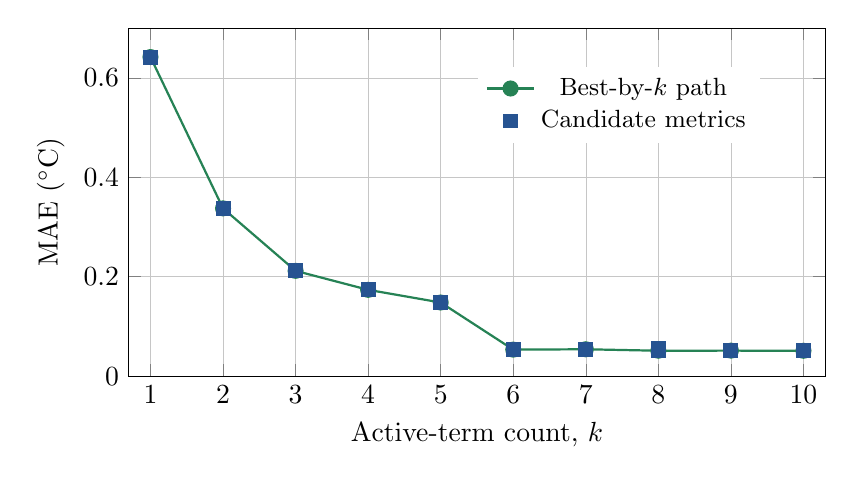
\begin{tikzpicture}
\begin{axis}[
    width=0.86\linewidth,
    height=6.0cm,
    xlabel={Active-term count, $k$},
    ylabel={MAE ($^\circ$C)},
    xmin=0.7, xmax=10.3,
    ymin=0, ymax=0.70,
    xtick={1,2,3,4,5,6,7,8,9,10},
    grid=both,
    grid style={line width=.1pt, draw=gray!25},
    major grid style={line width=.2pt,draw=gray!45},
    legend style={at={(0.50,0.78)},anchor=west,draw=none,fill=white,font=\small},
]
\addplot[
    color=bestGreen,
    thick,
    mark=*,
    mark size=2.5pt
] coordinates {
    (1,0.6420)
    (2,0.3375)
    (3,0.2118)
    (4,0.1736)
    (5,0.1481)
    (6,0.0533)
    (7,0.0540)
    (8,0.05107)
    (9,0.05128)
    (10,0.05098)
};
\addlegendentry{Best-by-$k$ path}
\addplot[
    only marks,
    color=anchorBlue,
    mark=square*,
    mark size=2.5pt
] coordinates {
    (1,0.6420)
    (2,0.3375)
    (3,0.2118)
    (4,0.1736)
    (5,0.1481)
    (6,0.0533)
    (7,0.0540)
    (8,0.0548)
    (8,0.0541)
    (8,0.0520)
    (8,0.0513)
    (8,0.05107)
    (9,0.05128)
    (10,0.05098)
};
\addlegendentry{Candidate metrics}
\end{axis}
\end{tikzpicture}
\caption{Complexity-path summary. Anchor metrics cluster around the eight-term structures, while the 10-term alternative is only marginally better than MIX8B.}
\end{figure}

\subsection{Formula Notation and Term-Level Interpretation}

\noindent
The equations below should be read as analytical pressure-coordinate approximations fitted or evaluated against the observed temperature profile.
Each candidate uses a small set of basis terms to represent different parts of the vertical structure, and the comparison is based on both evaluation error and parsimony.
The coefficient signs and magnitudes are therefore interpreted as fitted contributions within the complete formula, not as isolated causal effects.

\vspace{0.35em}
\begingroup
\small
\setlength{\tabcolsep}{5pt}
\renewcommand{\arraystretch}{1.18}
\begin{tabular}{L{3.2cm}L{4.4cm}L{7.0cm}}
\toprule
Symbol or term & Definition & Interpretation in the analytical profile \\
\midrule
$\hat{T}(P)$ & Fitted temperature at pressure $P$ & Model output used to reconstruct the temperature--pressure relationship. \\
$P$ & Pressure in dbar & Primary vertical coordinate. Larger $P$ corresponds to deeper water. \\
$k$ & Active-term count including the intercept & Complexity index used to compare candidate analytical structures. \\
$x,z$ & Standardized pressure coordinates & Center and scale pressure to improve numerical conditioning for polynomial and mixed polynomial terms. \\
$u$ & Rescaled pressure coordinate on approximately $[-1,1]$ & Coordinate used by the Chebyshev basis to reduce high-order polynomial instability. \\
$\ln(P)$ and $\sqrt{P}$ & Smooth nonlinear pressure terms & Capture broad vertical curvature that cannot be represented by a purely linear trend. \\
$\exp(-P/\tau)$ & Exponential decay term with scale $\tau$ & Represents rapidly weakening near-surface or intermediate-depth contributions. \\
$1/(P+c)$ & Shifted reciprocal pressure term & Adds strong shallow-pressure curvature while remaining bounded by the positive offset $c$. \\
$(P-\kappa)_+$ & ReLU hinge with knot $\kappa$ & Allows a slope change after a prescribed pressure threshold. \\
$L_{\kappa,s}(P)$ & Sigmoid transition centered at $\kappa$ with smoothness $s$ & Represents a smooth layer transition such as thermocline-like curvature. \\
$T_i(u)$ & $i$th Chebyshev polynomial mode & Provides numerically stable global polynomial modes over the rescaled pressure interval. \\
\bottomrule
\end{tabular}
\endgroup

\vspace{0.55em}
\noindent
In this catalogue, polynomial models mainly test how far global curvature alone can explain the profile.
Mixed-feature models combine broad background terms with decay and reciprocal terms, making them more suitable for profiles with shallow curvature and deep stabilization.
Piecewise and sigmoid-transition models test whether explicit layer-transition terms improve the fit enough to justify the additional complexity.

\clearpage
\subsection{Equation Definitions}

\noindent
Throughout, $P$ is pressure in dbar.
For standardized polynomial forms, $x=(P-1641.2335)/990.7445$.
For orthogonal and transition-basis equations, $u=2(P-100)/(4500-100)-1$, $(a)_+=\max(a,0)$ and $L_{\kappa,s}(P)=\{1+\exp[-(P-\kappa)/s]\}^{-1}$.

\vspace{0.35em}
\noindent\textbf{CONST1, $k=1$.}
\[
\hat{T}_{\mathrm{CONST1}}(P)=2.204.
\]
\noindent\emph{Explanation.}
This is the no-structure baseline. It represents only the mean thermal level and ignores all pressure-dependent stratification, so it defines the lower bound for useful profile reconstruction.

\vspace{0.35em}
\noindent\textbf{LIN2, $k=2$.}
\[
\hat{T}_{\mathrm{LIN2}}(P)=4.400-7.05\times10^{-4}P.
\]
\noindent\emph{Explanation.}
The linear trend adds a monotonic cooling-with-pressure component. It can describe the broad decrease of temperature with depth, but it cannot represent mixed-layer curvature, thermocline transition or deep asymptotic behaviour.

\vspace{0.35em}
\noindent\textbf{POLY2, $k=3$.}
\[
\hat{T}_{\mathrm{POLY2}}(P)=5.12742481
-2.64606596\times10^{-3}P
+5.35595691\times10^{-7}P^2.
\]
\noindent\emph{Explanation.}
The quadratic term adds a single global curvature to the pressure trend. This improves on the linear model but forces the whole water column to share one smooth curvature, which is too rigid for layered ocean thermal structure.

\vspace{0.35em}
\noindent\textbf{MIX4S, $k=4$.}
\[
\hat{T}_{\mathrm{MIX4S}}(P)=
7.23196288
-0.83859309\ln(P)
+0.02043606\sqrt{P}
+1.68598290\exp(-P/1000).
\]
\noindent\emph{Explanation.}
This seed model introduces physically interpretable nonlinear pressure components. The logarithmic and square-root terms describe broad profile curvature, while the exponential decay term gives the model a first mechanism for upper-ocean attenuation.

\vspace{0.35em}
\noindent\textbf{POLY4, $k=5$.}
\[
\begin{aligned}
\hat{T}_{\mathrm{POLY4}}(P)=&\,5.05404204
-2.26920822\times10^{-3}P
-3.96617497\times10^{-8}P^2 \\
&+3.37214976\times10^{-10}P^3
-6.71345918\times10^{-14}P^4.
\end{aligned}
\]
\noindent\emph{Explanation.}
The quartic polynomial increases flexibility by adding higher-order global curvature. It can reduce bias relative to low-order polynomials, but the basis remains purely algebraic and does not separately encode near-surface transitions or deep stabilization.

\vspace{0.35em}
\noindent\textbf{ZPOLY5, $k=6$.}
\[
\begin{aligned}
\hat{T}_{\mathrm{ZPOLY5}}(P)=&\,2.20411614
-0.86369338x
+0.41811779x^2
-0.08912643x^3 \\
&-0.00667122x^4
+0.00535626x^5.
\end{aligned}
\]
\noindent\emph{Explanation.}
Standardization improves numerical conditioning and allows the fifth-order polynomial to fit the main profile curvature more effectively. Its strong performance shows that normalization matters, although the representation is still a flexible empirical curve rather than a structured pressure-coordinate decomposition.

\vspace{0.35em}
\noindent\textbf{ZPOLY6, $k=7$.}
\[
\begin{aligned}
\hat{T}_{\mathrm{ZPOLY6}}(P)=&\,2.20278856
-0.87714145x
+0.42640403x^2
-0.06258684x^3 \\
&-0.01749463x^4
-0.00448305x^5
+0.00410846x^6.
\end{aligned}
\]
\noindent\emph{Explanation.}
The sixth-order standardized polynomial adds one more curvature degree of freedom. Its similar or slightly worse MAE compared with ZPOLY5 indicates that adding polynomial order alone does not guarantee better profile reconstruction.

\vspace{0.35em}
\noindent\textbf{CHEB8, $k=8$.}
\[
\begin{aligned}
\hat{T}_{\mathrm{CHEB8}}(P)=&\,2.206
-0.835T_1(u)
+0.421T_2(u)
-0.090T_3(u) \\
&-0.008T_4(u)
+0.006T_5(u)
-0.003T_6(u)
+0.002T_7(u).
\end{aligned}
\]
\noindent\emph{Explanation.}
The Chebyshev basis represents the full-depth profile with orthogonal polynomial modes. This improves numerical stability over raw high-order polynomials, but the terms remain global modes and are not directly tied to specific ocean-layer transitions.

\vspace{0.35em}
\noindent\textbf{RELU8, $k=8$.}
\[
\begin{aligned}
\hat{T}_{\mathrm{RELU8}}(P)=&\,5.18
-1.05\times10^{-3}P
+1.80\times10^{-3}(P-200)_+ \\
&-1.20\times10^{-3}(P-500)_+
+4.50\times10^{-4}(P-1000)_+ \\
&-1.80\times10^{-4}(P-1800)_+
+8.00\times10^{-5}(P-2800)_+ \\
&-3.00\times10^{-5}(P-3800)_+ .
\end{aligned}
\]
\noindent\emph{Explanation.}
The ReLU spline form divides the pressure axis into piecewise linear regimes. It is useful for approximating layer breaks and slope changes, but its knots impose sharp structural changes that may not reflect smooth thermodynamic transitions.

\vspace{0.35em}
\noindent\textbf{SIG8, $k=8$.}
\[
\begin{aligned}
\hat{T}_{\mathrm{SIG8}}(P)=&\,5.05
-6.20\times10^{-4}P
-1.12L_{250,70}(P)
-0.75L_{500,120}(P) \\
&-0.43L_{900,180}(P)
-0.26L_{1500,260}(P)
-0.12L_{2500,400}(P)
-0.07L_{3500,550}(P).
\end{aligned}
\]
\noindent\emph{Explanation.}
The sigmoid-transition basis replaces sharp knots with smooth pressure transitions. It is well suited to mixed-layer and thermocline gradients, but several transition terms can become redundant when the profile is already smooth at depth.

\vspace{0.35em}
\noindent\textbf{MIX8A, $k=8$.}
\[
\begin{aligned}
\hat{T}_{\mathrm{MIX8A}}(P)=&\,72.5243001
+130.024309z
-1.45894798z^2
+0.148251154z^3 \\
&+23.8341486\ln(P)
-6.13065083\sqrt{P}
+\frac{2610.76502}{P}
-9.36352770z\ln(P).
\end{aligned}
\]
\[
z=\frac{P-1641.2335}{990.7445}.
\]
\noindent\emph{Explanation.}
MIX8A combines standardized polynomial terms with logarithmic, square-root, reciprocal and interaction components. It captures both normalized background curvature and pressure-dependent nonlinear structure, but the cross term and $1/P$ component make the expression less stable near shallow pressures.

\vspace{0.35em}
\noindent\textbf{MIX8B, $k=8$, current recommended backbone.}
\[
\begin{aligned}
\hat{T}_{\mathrm{MIX8B}}(P)=&-356.873
+0.0125047P
+62.2025\ln(P)
-3.35576\sqrt{P} \\
&+20.0563\exp(-P/500)
+14.8832\exp(-P/1200) \\
&+\frac{10011.3}{P+50}
+\frac{7576.48}{P+500}.
\end{aligned}
\]
\noindent\emph{Explanation.}
MIX8B separates the profile into complementary pressure-coordinate components. The linear, logarithmic and square-root terms describe the broad vertical background; the two exponential terms capture rapid upper and intermediate decay; and the reciprocal terms constrain near-surface curvature while allowing deep-pressure stabilization.

\vspace{0.35em}
\noindent\textbf{PL9, $k=9$.}
\[
\begin{aligned}
\hat{T}_{\mathrm{PL9}}(P)=&\,2.214
-0.872x
+0.421x^2
-0.061x^3
-0.019x^4 \\
&-0.004x^5
+0.004x^6
+0.012\ln(P)
-0.006x\ln(P).
\end{aligned}
\]
\noindent\emph{Explanation.}
PL9 extends the standardized polynomial family with logarithmic interaction terms. It tests whether extra mixed polynomial-log flexibility can improve the profile fit, but the additional interaction mainly increases structural complexity and may duplicate curvature already captured by the lower-order terms.

\vspace{0.35em}
\noindent\textbf{SIG10, $k=10$.}
\[
\begin{aligned}
\hat{T}_{\mathrm{SIG10}}(P)=&\,4.820
-6.4\times10^{-4}P
-0.180\ln(P)
+0.036\sqrt{P} \\
&+0.42L_{250,80}(P)
+0.31L_{500,120}(P)
-0.22L_{850,180}(P) \\
&+0.15L_{1300,250}(P)
-0.11L_{2200,350}(P)
+0.08L_{3300,500}(P).
\end{aligned}
\]
\noindent\emph{Explanation.}
SIG10 uses multiple smooth transition functions distributed across the pressure column. It may slightly improve numerical accuracy by fitting local transition regions, but the gain is small relative to the extra terms, making it less attractive as a parsimonious analytical backbone.

\subsection{Suggested Reporting Logic}

\noindent
The comparison shows that low-order polynomials are insufficient, whereas compact nonlinear pressure-coordinate structures reduce errors to approximately 0.052--0.055$^\circ$C.
Among all eight-term candidates, MIX8B gives the strongest performance.
The additional candidate fits serve as a complexity-path sensitivity check: a 10-term transition model may be numerically similar or slightly better, but the gain is marginal relative to the additional complexity.
This supports presenting MIX8B as the parsimonious analytical backbone for Ocean-TP.

\clearpage
\section{Mixed-B Term-Count Evolution}
\label{sec:mixb-term-count-evolution}

\noindent\textcolor{noteRed}{\textbf{Experimental-result note.}}
This section records the Mixed-B term-count evolution obtained from fitting and evaluation.
The plotted values, tabulated metrics and incremental changes summarize the sequential improvement along the Mixed-B term-count path.
Here $k$ counts all active algebraic terms, including the intercept.
The first-term point is the intercept-only null baseline; when the intercept is fitted as the sample mean, $R^2=0$ by definition.
The first pressure-dependent term enters at $k=2$, and the eighth-term point is the current Mixed-B anchor: MAE = 0.05107$^\circ$C, RMSE = 0.11189$^\circ$C and $R^2=0.98407$.

\subsection{Experimental Term-Count Metric Path}

\begin{figure}[htbp]
\centering
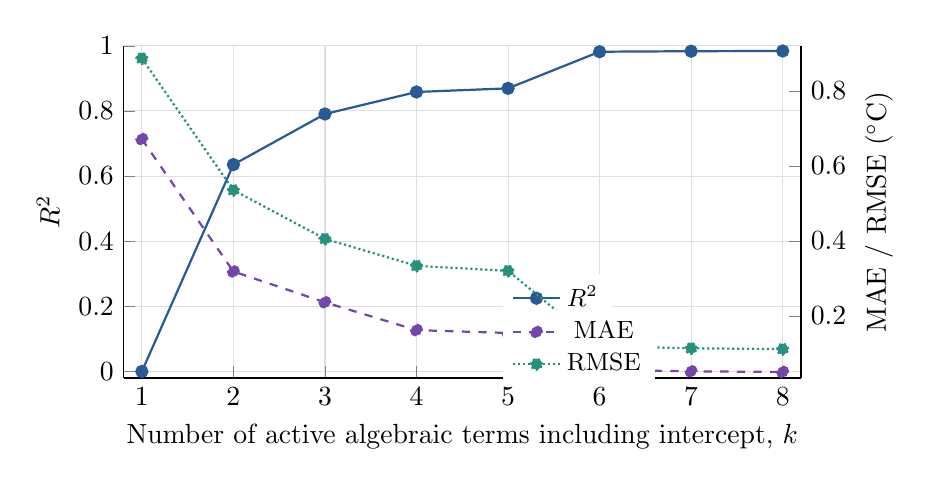
\begin{tikzpicture}
\begin{axis}[
    width=0.84\linewidth,
    height=5.8cm,
    xlabel={Number of active algebraic terms including intercept, $k$},
    ylabel={$R^2$},
    xmin=0.8, xmax=8.2,
    ymin=-0.02, ymax=1.00,
    xtick={1,2,3,4,5,6,7,8},
    ymajorgrids=true,
    xmajorgrids=true,
    grid style={draw=gray!25},
    axis y line*=left,
    axis x line*=bottom,
    legend style={at={(0.56,0.24)},anchor=west,draw=none,fill=white,font=\small},
]
\addplot[color=rTwoBlue,mark=*,thick] coordinates {
    (1,0.00000)
    (2,0.63529)
    (3,0.79057)
    (4,0.85824)
    (5,0.86939)
    (6,0.98183)
    (7,0.98344)
    (8,0.98407)
};
\addlegendentry{$R^2$}
\end{axis}
\begin{axis}[
    width=0.84\linewidth,
    height=5.8cm,
    xmin=0.8, xmax=8.2,
    ymin=0.035, ymax=0.92,
    xtick={1,2,3,4,5,6,7,8},
    ylabel={MAE / RMSE ($^\circ$C)},
    axis y line*=right,
    axis x line=none,
    legend style={at={(0.56,0.09)},anchor=west,draw=none,fill=white,font=\small},
]
\addplot[color=maePurple,mark=*,thick,dashed] coordinates {
    (1,0.67142)
    (2,0.31876)
    (3,0.23658)
    (4,0.16243)
    (5,0.15492)
    (6,0.05638)
    (7,0.05271)
    (8,0.05107)
};
\addlegendentry{MAE}
\addplot[color=rmseGreen,mark=*,thick,densely dotted] coordinates {
    (1,0.88659)
    (2,0.53542)
    (3,0.40573)
    (4,0.33381)
    (5,0.32041)
    (6,0.11952)
    (7,0.11409)
    (8,0.11189)
};
\addlegendentry{RMSE}
\end{axis}
\end{tikzpicture}
\caption{Term-count evolution of the Mixed-B analytical backbone. The first point is the intercept-only null baseline. Error decreases strongly after pressure dependence is introduced, improves through the nonlinear curvature terms, drops again when the dual-decay structure is completed, and then reaches a low-error plateau from six to eight terms.}
\end{figure}

\begingroup
\small
\setlength{\tabcolsep}{4pt}
\renewcommand{\arraystretch}{1.12}
\begin{longtable}{C{0.55cm}L{3.05cm}L{5.6cm}ccc}
\caption{Term-by-term evolution of the Mixed-B equation. The term count $k$ includes the intercept.}\\
\toprule
$k$ & Newly added basis term & Basis composition after adding the term & MAE ($^\circ$C) & RMSE ($^\circ$C) & $R^2$ \\
\midrule
\endfirsthead
\toprule
$k$ & Newly added basis term & Basis composition after adding the term & MAE ($^\circ$C) & RMSE ($^\circ$C) & $R^2$ \\
\midrule
\endhead
1 & Intercept-only null baseline & $c_0^{(1)}$ & 0.67142 & 0.88659 & 0.00000 \\
2 & Linear pressure, $P$ & $c_0^{(2)}+c_1^{(2)}P$ & 0.31876 & 0.53542 & 0.63529 \\
3 & Logarithmic curvature, $\ln P$ & $c_0^{(3)}+c_1^{(3)}P+c_2^{(3)}\ln P$ & 0.23658 & 0.40573 & 0.79057 \\
4 & Square-root curvature, $\sqrt{P}$ & $c_0^{(4)}+c_1^{(4)}P+c_2^{(4)}\ln P+c_3^{(4)}\sqrt{P}$ & 0.16243 & 0.33381 & 0.85824 \\
5 & Fast exponential decay, $e^{-P/500}$ & $\hat{T}_4(P)+c_4^{(5)}e^{-P/500}$ & 0.15492 & 0.32041 & 0.86939 \\
6 & Slow exponential decay, $e^{-P/1200}$ & $\hat{T}_5(P)+c_5^{(6)}e^{-P/1200}$ & 0.05638 & 0.11952 & 0.98183 \\
7 & Near-surface reciprocal, $(P+50)^{-1}$ & $\hat{T}_6(P)+c_6^{(7)}(P+50)^{-1}$ & 0.05271 & 0.11409 & 0.98344 \\
8 & Stabilizing reciprocal, $(P+500)^{-1}$ & $\hat{T}_7(P)+c_7^{(8)}(P+500)^{-1}$ & \textbf{0.05107} & \textbf{0.11189} & \textbf{0.98407} \\
\bottomrule
\end{longtable}
\endgroup

\subsection{Incremental Error Reduction}

\begingroup
\small
\setlength{\tabcolsep}{5pt}
\renewcommand{\arraystretch}{1.12}
\begin{tabular}{C{1.2cm}cccL{7.2cm}}
\toprule
Step & $\Delta$MAE & $\Delta$RMSE & $\Delta R^2$ & Interpretation \\
\midrule
1$\rightarrow$2 & 0.35266 & 0.35117 & 0.63529 & Introducing pressure dependence gives the largest overall improvement because the model first moves beyond the intercept-only null baseline and acquires a vertical coordinate trend. \\
2$\rightarrow$3 & 0.08218 & 0.12969 & 0.15528 & Adding logarithmic curvature provides a substantial nonlinear improvement and captures broad upper-to-intermediate profile bending. \\
3$\rightarrow$4 & 0.07415 & 0.07192 & 0.06767 & The square-root term adds a second smooth curvature scale and further refines the profile. \\
4$\rightarrow$5 & 0.00751 & 0.01340 & 0.01115 & The first exponential term introduces fast pressure attenuation and gives a smaller transition refinement. \\
5$\rightarrow$6 & 0.09854 & 0.20089 & 0.11244 & The second exponential decay creates the second major low-error transition, indicating that a slower intermediate-depth scale is essential in the fitted path. \\
6$\rightarrow$7 & 0.00367 & 0.00543 & 0.00161 & The near-surface reciprocal acts mainly as a local correction after the dominant structure is already captured. \\
7$\rightarrow$8 & 0.00164 & 0.00220 & 0.00063 & The stabilizing reciprocal gives a final small refinement and completes the compact Mixed-B backbone. \\
\bottomrule
\end{tabular}
\endgroup

\subsection{Term-by-Term Interpretation}

\noindent\textbf{$k=1$: intercept.}
The first term provides the intercept-only null baseline and acts as the reference state for the pressure-coordinate profile.
Because this model predicts only the sample mean temperature, its $R^2$ is zero by definition.
It cannot represent vertical stratification, so its error is substantially larger than all pressure-dependent candidates.

\vspace{0.25em}
\noindent\textbf{$k=2$: linear pressure term.}
Adding $P$ introduces the first-order cooling tendency with pressure.
This term captures the broad vertical trend but remains too simple for thermocline curvature.

\vspace{0.25em}
\noindent\textbf{$k=3$: logarithmic term.}
The addition of $\ln P$ produces a strong nonlinear improvement in the complexity path.
It gives the equation a compact way to represent nonlinear curvature across the upper and intermediate water column, explaining the substantial increase in $R^2$ and the reduction in both MAE and RMSE.

\vspace{0.25em}
\noindent\textbf{$k=4$: square-root term.}
The $\sqrt{P}$ component adds a second smooth curvature scale.
Together with $\ln P$, it refines the background profile shape without introducing abrupt transitions.

\vspace{0.25em}
\noindent\textbf{$k=5$ and $k=6$: dual exponential decays.}
The $e^{-P/500}$ and $e^{-P/1200}$ terms describe fast and slower attenuation with pressure.
In the fitted path, the second exponential term marks the transition into the low-error regime, indicating that multi-scale decay is essential for recovering the dominant vertical thermal structure.

\vspace{0.25em}
\noindent\textbf{$k=7$ and $k=8$: reciprocal stabilization.}
The $(P+50)^{-1}$ and $(P+500)^{-1}$ terms provide localized near-surface curvature while remaining bounded at depth.
Their incremental gains are smaller than the earlier terms, but they complete the compact Mixed-B backbone and improve full-profile coherence.

\subsection{Final Mixed-B Equation and Reporting Logic}

\[
\begin{aligned}
\hat{T}_{8}^{B}(P)=&-356.873
+0.0125047P
+62.2025\ln(P)
-3.35576\sqrt{P} \\
&+20.0563\exp(-P/500)
+14.8832\exp(-P/1200) \\
&+\frac{10011.3}{P+50}
+\frac{7576.48}{P+500}.
\end{aligned}
\]

\noindent
This final form can be described as an explicit pressure-coordinate backbone with three functional roles: broad background structure from $P$, $\ln P$ and $\sqrt{P}$; multi-scale decay from the two exponential terms; and near-surface plus deep-pressure stabilization from the reciprocal terms.
The Mixed-B basis can therefore be reported as a term-count path from an intercept-only null baseline to a compact eight-term pressure-coordinate representation.
Errors decrease strongly after pressure dependence is introduced, continue improving through the nonlinear curvature terms, enter a low-error regime once the dual exponential terms are included, and then receive smaller but consistent refinements from the reciprocal components.

\clearpage
\section{Baseline Metrics for Result 1}
\label{sec:baseline-metrics-result1}

\noindent\textcolor{noteRed}{\textbf{Complete-data note.}}
This section reports the complete baseline metric record supporting the final benchmark comparison in Result 1.
The row-level source catalogue uses the same 10k evaluation split, with 8,000 training samples and 2,000 test samples.
The source record contains one Mixed-B-only regression-fit analytical control and 298 data-driven benchmark configurations.
For clarity, \textit{Ocean-TP optimized Mixed-B} denotes the complete optimized reference result reported in the main manuscript, and is used here as the representative Ocean-TP model result.
By contrast, \textit{Mixed-B-only regression fit} denotes the analytical control obtained by an ordinary regression fit using only the Mixed-B functional form.
The full Ocean-TP optimized Mixed-B result is shown as a manuscript-level reference in the representative visualization, but is not counted as one of the 298 conventional benchmark configurations.
Rows preserve the source metric-record order, and the category labels are reported in English as analytical control, classical regression and deep regression.
The metrics are displayed to five decimal places for consistency with the preceding tables.

\subsection{Representative Model-Family Visualization}

\noindent
The manuscript Table 2 reports the Ocean-TP optimized Mixed-B result together with the best-performing representative entry from each major model family.
Figure~\ref{fig:representative-baseline-mae} visualizes those representative entries by MAE, including the full Ocean-TP optimized Mixed-B reference and the Mixed-B-only regression-fit analytical control, while the complete row-level metric catalogue is retained in Table~\ref{tab:complete-baseline-metrics-result1}.

\begin{figure}[htbp]
\centering
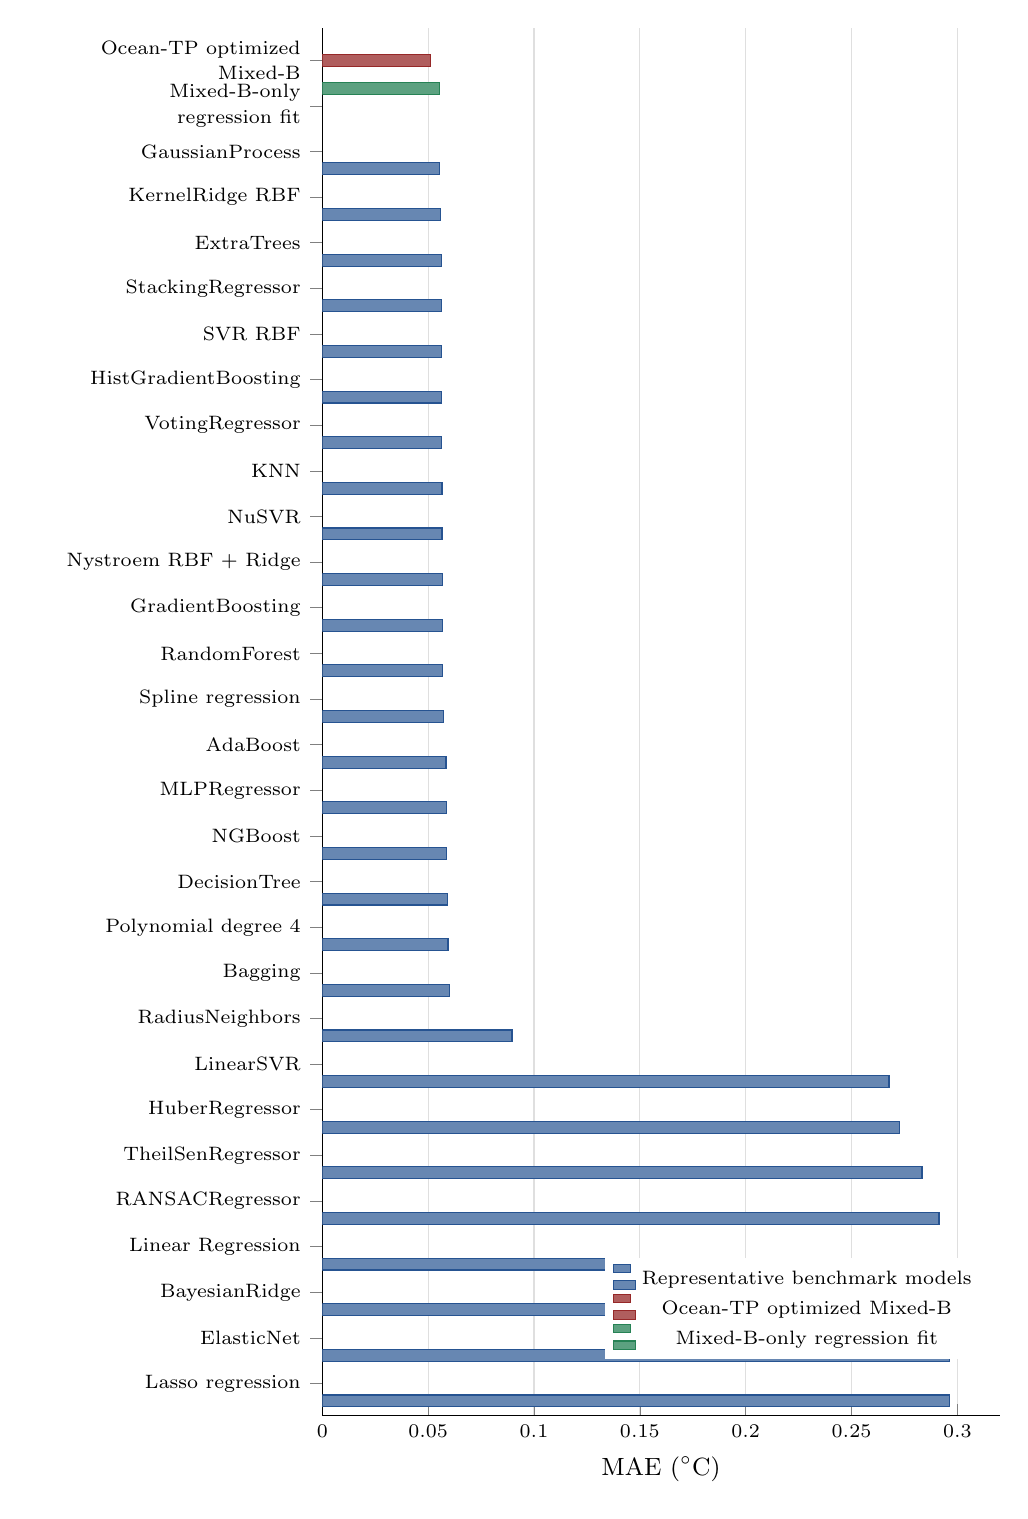
\begin{tikzpicture}
\begin{axis}[
    xbar,
    width=0.84\linewidth,
    height=19.2cm,
    xmin=0, xmax=0.32,
    xlabel={MAE ($^\circ$C)},
    xtick={0,0.05,0.10,0.15,0.20,0.25,0.30},
    scaled x ticks=false,
    ytick={1,2,3,4,5,6,7,8,9,10,11,12,13,14,15,16,17,18,19,20,21,22,23,24,25,26,27,28,29,30},
    yticklabels={
        Lasso regression,
        ElasticNet,
        BayesianRidge,
        Linear Regression,
        RANSACRegressor,
        TheilSenRegressor,
        HuberRegressor,
        LinearSVR,
        RadiusNeighbors,
        Bagging,
        Polynomial degree 4,
        DecisionTree,
        NGBoost,
        MLPRegressor,
        AdaBoost,
        Spline regression,
        RandomForest,
        GradientBoosting,
        Nystroem RBF + Ridge,
        NuSVR,
        KNN,
        VotingRegressor,
        HistGradientBoosting,
        SVR RBF,
        StackingRegressor,
        ExtraTrees,
        KernelRidge RBF,
        GaussianProcess,
        \shortstack[r]{Mixed-B-only\\regression fit},
        \shortstack[r]{Ocean-TP optimized\\Mixed-B}
    },
    ymin=0.3, ymax=30.7,
    yticklabel style={font=\scriptsize,text width=3.35cm,align=right},
    xticklabel style={font=\scriptsize,/pgf/number format/fixed,/pgf/number format/precision=2},
    label style={font=\small},
    xmajorgrids=true,
    grid style={draw=gray!25},
    axis x line*=bottom,
    axis y line*=left,
    legend style={at={(0.98,0.04)},anchor=south east,draw=none,fill=white,font=\scriptsize},
    bar width=4.3pt,
]
\addplot[fill=anchorBlue!70,draw=anchorBlue] coordinates {
    (0.05542,28)
    (0.05578,27)
    (0.05623,26)
    (0.05623,25)
    (0.05642,24)
    (0.05644,23)
    (0.05648,22)
    (0.05654,21)
    (0.05658,20)
    (0.05684,19)
    (0.05688,18)
    (0.05691,17)
    (0.05727,16)
    (0.05843,15)
    (0.05850,14)
    (0.05865,13)
    (0.05903,12)
    (0.05938,11)
    (0.06008,10)
    (0.08961,9)
    (0.26772,8)
    (0.27282,7)
    (0.28330,6)
    (0.29134,5)
    (0.29625,4)
    (0.29626,3)
    (0.29629,2)
    (0.29636,1)
};
\addlegendentry{Representative benchmark models}
\addplot[fill=noteRed!75,draw=noteRed] coordinates {
    (0.05107,30)
};
\addlegendentry{Ocean-TP optimized Mixed-B}
\addplot[fill=bestGreen!75,draw=bestGreen] coordinates {
    (0.05535,29)
};
\addlegendentry{Mixed-B-only regression fit}
\end{axis}
\end{tikzpicture}
\caption{Representative baseline MAE comparison for the Result 1 benchmark. The plotted entries correspond to the condensed manuscript benchmark table, which retains the best-performing member of each major model family from the broader 298-configuration benchmark catalogue, together with the full Ocean-TP optimized Mixed-B reference and the Mixed-B-only regression control.}
\label{fig:representative-baseline-mae}
\end{figure}

\subsection{Interpretive Discussion of Representative Model Families}

\noindent
The representative benchmark should be read as a family-level stress test rather than as a search for a single numerical winner.
The 298 data-driven configurations cover linear, robust, polynomial, kernel, neighborhood, tree-ensemble, boosting, probabilistic and shallow neural-network regressors.
The Mixed-B-only row is included as an analytical control that fits the Ocean-TP selected basis as a conventional regression model.
Therefore, the key comparison is not only whether a model can reach a low MAE, but also what type of structure is required to do so and whether the resulting representation remains interpretable.

\vspace{0.25em}
\noindent\textbf{Near-frontier smooth nonlinear models.}
GaussianProcess, KernelRidge, SVR, NuSVR, Nystroem RBF + Ridge and KNN all enter the leading error band when configured with smooth radial-basis or local-neighborhood structure.
Their representative MAE values lie close to the Mixed-B-only regression control, mostly between approximately 0.055 and 0.057$^\circ$C.
This indicates that the dominant pressure-temperature relationship in the 10k split is smooth enough for kernel and local interpolation methods to recover effectively.
At the same time, these methods remain primarily algorithmic function approximators: they can match the curve but do not directly expose a compact pressure-coordinate equation.
The Mixed-B-only result is therefore important because it reaches the same accuracy band with an explicit eight-term structure rather than through an implicit kernel expansion or local averaging rule.

\vspace{0.25em}
\noindent\textbf{Tree and ensemble models.}
ExtraTrees, HistGradientBoosting, GradientBoosting, RandomForest, VotingRegressor, StackingRegressor, AdaBoost, Bagging and NGBoost form a second group of strong nonlinear learners.
The best tree-ensemble entries also remain within the narrow high-skill band, with representative MAE values near 0.056--0.060$^\circ$C.
This confirms that the benchmark is not biased toward one modeling family: several independent algorithmic routes can approximate the same vertical profile.
However, the ensemble models distribute the reconstruction across many trees, boosting stages or stacked components.
Their accuracy therefore supports the existence of a learnable nonlinear pressure structure, but it does not provide the same direct symbolic decomposition into background trend, multi-scale decay and reciprocal stabilization that the Mixed-B equation provides.

\vspace{0.25em}
\noindent\textbf{Polynomial and spline baselines.}
The polynomial and spline models help separate smooth global curvature from more structured physical representation.
Spline regression and the best polynomial representative retain reasonable accuracy, but their role is mainly to show that generic smoothness alone is not the whole explanation.
The complete catalogue shows that polynomial performance is degree-sensitive: moderate polynomial order can be competitive, whereas over-extended orders degrade markedly.
This behavior is consistent with the interpretation from Section~\ref{sec:analytical-complexity-path}: adding algebraic flexibility alone does not guarantee a better reconstruction.
The Mixed-B basis improves this situation by combining algebraic curvature with exponential and reciprocal pressure terms, giving the equation a more targeted way to represent upper-ocean transition and deep-pressure stabilization.

\vspace{0.25em}
\noindent\textbf{Linear and robust statistical regressors.}
Linear Regression, BayesianRidge, ElasticNet, Lasso, LinearSVR, HuberRegressor, TheilSenRegressor and RANSACRegressor occupy a clearly higher-error regime.
Their representative MAE values remain around 0.27--0.30$^\circ$C for the linear or robust-linear cases, far above the leading nonlinear group.
This gap is useful because it shows that the benchmark difficulty is not mainly caused by a few outliers or by noise sensitivity.
Robust estimators can reduce the influence of anomalous points, but they do not solve the core structural problem: the vertical temperature profile is nonlinear in pressure and contains curvature regimes that cannot be represented by a single global slope.
The poor performance of these baselines therefore strengthens the claim that pressure-coordinate nonlinearity is essential.

\vspace{0.25em}
\noindent\textbf{Neighborhood-scale sensitivity.}
The nearest-neighbor family illustrates the importance of scale choice.
KNN with a well-selected neighborhood reaches the leading band, while RadiusNeighbors is much more sensitive to the selected radius and remains outside the top group in the representative comparison.
This contrast is useful because it shows that local methods can be very accurate only when the locality scale is well matched to the density and curvature of the pressure-temperature data.
The Mixed-B-only control avoids this explicit neighborhood-scale tuning by representing the profile through fixed analytical basis functions.

\vspace{0.25em}
\noindent\textbf{Neural and feature-mapped baselines.}
The MLP regressor representative reaches a competitive MAE near 0.0585$^\circ$C, indicating that a shallow neural network can learn the smooth one-dimensional mapping with reasonable accuracy.
The complete catalogue also records a FourierFeatures+Ridge entry with much poorer performance, which shows that adding a feature map does not automatically improve the reconstruction unless the representation is well matched to the target structure.
For this benchmark, the neural and feature-mapped baselines are therefore best interpreted as flexible comparators, not as the central explanation of the observed accuracy.
Ocean-TP uses the selected Mixed-B structure as the optimized pressure-coordinate representation before any subsequent constrained refinement.

\vspace{0.25em}
\noindent\textbf{Implication for the Result 1 claim.}
The central message of this benchmark is not that data-driven models are weak.
On the contrary, several modern nonlinear regressors achieve very similar reconstruction errors.
The key point is that the Mixed-B-only regression control lies inside the same leading performance band while remaining compact, explicit and physically interpretable.
This gives the Result 1 benchmark a stronger interpretation: Ocean-TP does not rely on arbitrary curve fitting to reach the benchmark frontier.
It first identifies a low-dimensional analytical pressure-coordinate backbone, then reserves later model components for constrained refinement rather than replacing the physical structure with an opaque predictor.

\subsection{Complete Baseline Metric Catalogue}

\begingroup
\footnotesize
\setlength{\tabcolsep}{2.2pt}
\renewcommand{\arraystretch}{1.08}
\begin{longtable}{C{0.75cm}L{2.35cm}L{8.0cm}C{1.15cm}C{1.15cm}C{1.15cm}}
\caption{Complete baseline metrics for the representative 10k Result 1 benchmark evaluation. All rows use an 8,000 / 2,000 train-test split.}
\label{tab:complete-baseline-metrics-result1}\\
\toprule
No. & Category & Model & MAE & RMSE & $R^2$ \\
\midrule
\endfirsthead
\toprule
No. & Category & Model & MAE & RMSE & $R^2$ \\
\midrule
\endhead
1 & Analytical control & Mixed-B-only regression fit & 0.05535 & 0.10756 & 0.98469 \\
2 & Classical regression & Linear Regression & 0.29625 & 0.37017 & 0.81868 \\
3 & Classical regression & Polynomial Regression (deg=5) & 0.07097 & 0.13194 & 0.97697 \\
4 & Classical regression & SVR (RBF) & 0.05870 & 0.11422 & 0.98274 \\
5 & Classical regression & Random Forest & 0.06250 & 0.12158 & 0.98044 \\
6 & Classical regression & Spline Regression (B-spline, 10 knots) & 0.05727 & 0.11110 & 0.98367 \\
7 & Classical regression & Nystroem RBF + Ridge (Kriging approx) & 0.05684 & 0.11077 & 0.98376 \\
8 & Classical regression & Nystroem RBF(1024) + Ridge & 0.05684 & 0.11077 & 0.98376 \\
9 & Classical regression & KNN (k=25, distance) & 0.06507 & 0.12890 & 0.97802 \\
10 & Classical regression & Decision Tree (max\_depth=18) & 0.06406 & 0.12527 & 0.97923 \\
11 & Classical regression & ExtraTrees & 0.06512 & 0.12891 & 0.97801 \\
12 & Classical regression & ElasticNet & 0.29634 & 0.37015 & 0.81870 \\
13 & Classical regression & KernelRidge (RBF) & 0.05688 & 0.11093 & 0.98372 \\
14 & Classical regression & HistGradientBoosting & 0.05661 & 0.10873 & 0.98436 \\
15 & Classical regression & GradientBoosting & 0.05688 & 0.10999 & 0.98399 \\
16 & Classical regression & AdaBoost (Tree base) & 0.05843 & 0.11422 & 0.98274 \\
17 & Classical regression & Bagging (Tree base) & 0.06008 & 0.11593 & 0.98222 \\
18 & Classical regression & BayesianRidge & 0.29626 & 0.37017 & 0.81868 \\
19 & Classical regression & HuberRegressor & 0.27282 & 0.40239 & 0.78574 \\
20 & Classical regression & Lasso & 0.29636 & 0.37014 & 0.81871 \\
21 & Classical regression & LinearSVR & 0.26772 & 0.43354 & 0.75129 \\
22 & Classical regression & NuSVR (RBF) & 0.05717 & 0.11434 & 0.98270 \\
23 & Classical regression & SVR (poly, deg=3) & 0.61084 & 0.74108 & 0.27327 \\
24 & Classical regression & SGDRegressor & 0.29823 & 0.37001 & 0.81884 \\
25 & Classical regression & RANSACRegressor & 0.29134 & 0.52866 & 0.63018 \\
26 & Classical regression & TheilSenRegressor & 0.28330 & 0.48744 & 0.68560 \\
27 & Classical regression & RadiusNeighbors (radius=1.0) & 0.25219 & 0.34235 & 0.84491 \\
28 & Classical regression & KernelRidge (poly, deg=3) & 0.05978 & 0.11810 & 0.98155 \\
29 & Classical regression & GaussianProcess (RBF, subsample=2k) & 0.05568 & 0.10815 & 0.98452 \\
30 & Classical regression & GaussianProcess (Matern $\nu$=1.5, subsample=2k) & 0.05542 & 0.10814 & 0.98452 \\
31 & Classical regression & GaussianProcess (RationalQuadratic, subsample=2k) & 0.05554 & 0.10805 & 0.98455 \\
32 & Classical regression & VotingRegressor (LR+RF+SVR) & 0.11628 & 0.16437 & 0.96425 \\
33 & Classical regression & StackingRegressor (RF+SVR -> Ridge) & 0.05807 & 0.11263 & 0.98321 \\
34 & Classical regression & VotingRegressor (SVR+HGB+KernelRidge) & 0.05648 & 0.10973 & 0.98407 \\
35 & Classical regression & StackingRegressor (SVR+HGB+KernelRidge$\rightarrow$Ridge) & 0.05623 & 0.10842 & 0.98445 \\
36 & Classical regression & Polynomial Regression (deg=2) & 0.08221 & 0.13376 & 0.97632 \\
37 & Classical regression & Polynomial Regression (deg=3) & 0.05978 & 0.11810 & 0.98155 \\
38 & Classical regression & Polynomial Regression (deg=4) & 0.05938 & 0.11803 & 0.98157 \\
39 & Classical regression & Polynomial Regression (deg=6) & 0.13487 & 0.19623 & 0.94905 \\
40 & Classical regression & Polynomial Regression (deg=7) & 0.21484 & 0.28749 & 0.89063 \\
41 & Classical regression & Polynomial Regression (deg=8) & 0.29138 & 0.37408 & 0.81483 \\
42 & Classical regression & Polynomial Regression (deg=9) & 0.36236 & 0.45100 & 0.73085 \\
43 & Classical regression & Polynomial Regression (deg=10) & 0.42747 & 0.52025 & 0.64185 \\
44 & Classical regression & Polynomial Regression (deg=11) & 0.48949 & 0.58117 & 0.55306 \\
45 & Classical regression & Polynomial Regression (deg=12) & 0.53703 & 0.63110 & 0.47298 \\
46 & Classical regression & SVR (RBF,C=0.5,gamma=scale,eps=0.01) & 0.05766 & 0.12166 & 0.98041 \\
47 & Classical regression & SVR (RBF,C=0.5,gamma=scale,eps=0.05) & 0.05922 & 0.12081 & 0.98069 \\
48 & Classical regression & SVR (RBF,C=0.5,gamma=0.001,eps=0.01) & 0.26184 & 0.39930 & 0.78902 \\
49 & Classical regression & SVR (RBF,C=0.5,gamma=0.001,eps=0.05) & 0.26356 & 0.39071 & 0.79800 \\
50 & Classical regression & SVR (RBF,C=0.5,gamma=0.005,eps=0.01) & 0.10184 & 0.17411 & 0.95989 \\
51 & Classical regression & SVR (RBF,C=0.5,gamma=0.005,eps=0.05) & 0.10944 & 0.17834 & 0.95791 \\
52 & Classical regression & SVR (RBF,C=0.5,gamma=0.01,eps=0.01) & 0.08467 & 0.14934 & 0.97049 \\
53 & Classical regression & SVR (RBF,C=0.5,gamma=0.01,eps=0.05) & 0.08547 & 0.14648 & 0.97161 \\
54 & Classical regression & SVR (RBF,C=1.0,gamma=scale,eps=0.01) & 0.05736 & 0.11994 & 0.98096 \\
55 & Classical regression & SVR (RBF,C=1.0,gamma=scale,eps=0.05) & 0.05954 & 0.11910 & 0.98123 \\
56 & Classical regression & SVR (RBF,C=1.0,gamma=0.001,eps=0.01) & 0.25010 & 0.39067 & 0.79804 \\
57 & Classical regression & SVR (RBF,C=1.0,gamma=0.001,eps=0.05) & 0.25087 & 0.38456 & 0.80431 \\
58 & Classical regression & SVR (RBF,C=1.0,gamma=0.005,eps=0.01) & 0.08889 & 0.15672 & 0.96750 \\
59 & Classical regression & SVR (RBF,C=1.0,gamma=0.005,eps=0.05) & 0.09111 & 0.15501 & 0.96820 \\
60 & Classical regression & SVR (RBF,C=1.0,gamma=0.01,eps=0.01) & 0.08080 & 0.14254 & 0.97312 \\
61 & Classical regression & SVR (RBF,C=1.0,gamma=0.01,eps=0.05) & 0.08167 & 0.14050 & 0.97388 \\
62 & Classical regression & SVR (RBF,C=5.0,gamma=scale,eps=0.01) & 0.05681 & 0.11601 & 0.98219 \\
63 & Classical regression & SVR (RBF,C=5.0,gamma=scale,eps=0.05) & 0.05875 & 0.11548 & 0.98235 \\
64 & Classical regression & SVR (RBF,C=5.0,gamma=0.001,eps=0.01) & 0.18268 & 0.27946 & 0.89666 \\
65 & Classical regression & SVR (RBF,C=5.0,gamma=0.001,eps=0.05) & 0.18470 & 0.27564 & 0.89946 \\
66 & Classical regression & SVR (RBF,C=5.0,gamma=0.005,eps=0.01) & 0.08004 & 0.14054 & 0.97386 \\
67 & Classical regression & SVR (RBF,C=5.0,gamma=0.005,eps=0.05) & 0.08066 & 0.13845 & 0.97464 \\
68 & Classical regression & SVR (RBF,C=5.0,gamma=0.01,eps=0.01) & 0.06728 & 0.12696 & 0.97867 \\
69 & Classical regression & SVR (RBF,C=5.0,gamma=0.01,eps=0.05) & 0.07108 & 0.12832 & 0.97821 \\
70 & Classical regression & SVR (RBF,C=10.0,gamma=scale,eps=0.01) & 0.05657 & 0.11431 & 0.98271 \\
71 & Classical regression & SVR (RBF,C=10.0,gamma=scale,eps=0.05) & 0.05870 & 0.11422 & 0.98274 \\
72 & Classical regression & SVR (RBF,C=10.0,gamma=0.001,eps=0.01) & 0.10831 & 0.17924 & 0.95749 \\
73 & Classical regression & SVR (RBF,C=10.0,gamma=0.001,eps=0.05) & 0.11694 & 0.18471 & 0.95485 \\
74 & Classical regression & SVR (RBF,C=10.0,gamma=0.005,eps=0.01) & 0.07711 & 0.13642 & 0.97537 \\
75 & Classical regression & SVR (RBF,C=10.0,gamma=0.005,eps=0.05) & 0.07818 & 0.13503 & 0.97587 \\
76 & Classical regression & SVR (RBF,C=10.0,gamma=0.01,eps=0.01) & 0.06204 & 0.12220 & 0.98024 \\
77 & Classical regression & SVR (RBF,C=10.0,gamma=0.01,eps=0.05) & 0.06643 & 0.12385 & 0.97970 \\
78 & Classical regression & SVR (RBF,C=20.0,gamma=scale,eps=0.01) & 0.05642 & 0.11304 & 0.98309 \\
79 & Classical regression & SVR (RBF,C=20.0,gamma=scale,eps=0.05) & 0.05863 & 0.11272 & 0.98319 \\
80 & Classical regression & SVR (RBF,C=20.0,gamma=0.001,eps=0.01) & 0.08998 & 0.15790 & 0.96701 \\
81 & Classical regression & SVR (RBF,C=20.0,gamma=0.001,eps=0.05) & 0.09356 & 0.15786 & 0.96703 \\
82 & Classical regression & SVR (RBF,C=20.0,gamma=0.005,eps=0.01) & 0.07251 & 0.13121 & 0.97722 \\
83 & Classical regression & SVR (RBF,C=20.0,gamma=0.005,eps=0.05) & 0.07455 & 0.13129 & 0.97719 \\
84 & Classical regression & SVR (RBF,C=20.0,gamma=0.01,eps=0.01) & 0.06056 & 0.12026 & 0.98086 \\
85 & Classical regression & SVR (RBF,C=20.0,gamma=0.01,eps=0.05) & 0.06383 & 0.12117 & 0.98057 \\
86 & Classical regression & NuSVR (RBF,nu=0.25,C=1.0) & 0.06015 & 0.11884 & 0.98131 \\
87 & Classical regression & NuSVR (RBF,nu=0.25,C=5.0) & 0.05969 & 0.11554 & 0.98233 \\
88 & Classical regression & NuSVR (RBF,nu=0.25,C=10.0) & 0.05976 & 0.11400 & 0.98280 \\
89 & Classical regression & NuSVR (RBF,nu=0.5,C=1.0) & 0.05779 & 0.11959 & 0.98107 \\
90 & Classical regression & NuSVR (RBF,nu=0.5,C=5.0) & 0.05733 & 0.11561 & 0.98231 \\
91 & Classical regression & NuSVR (RBF,nu=0.5,C=10.0) & 0.05717 & 0.11434 & 0.98270 \\
92 & Classical regression & NuSVR (RBF,nu=0.75,C=1.0) & 0.05739 & 0.11995 & 0.98096 \\
93 & Classical regression & NuSVR (RBF,nu=0.75,C=5.0) & 0.05681 & 0.11599 & 0.98220 \\
94 & Classical regression & NuSVR (RBF,nu=0.75,C=10.0) & 0.05658 & 0.11427 & 0.98272 \\
95 & Classical regression & LinearSVR (C=0.1,eps=0.01) & 0.26777 & 0.43585 & 0.74863 \\
96 & Classical regression & LinearSVR (C=0.1,eps=0.05) & 0.26776 & 0.43345 & 0.75140 \\
97 & Classical regression & LinearSVR (C=1.0,eps=0.01) & 0.26773 & 0.43506 & 0.74955 \\
98 & Classical regression & LinearSVR (C=1.0,eps=0.05) & 0.26772 & 0.43354 & 0.75129 \\
99 & Classical regression & LinearSVR (C=10.0,eps=0.01) & 0.26782 & 0.43756 & 0.74665 \\
100 & Classical regression & LinearSVR (C=10.0,eps=0.05) & 0.26776 & 0.43354 & 0.75128 \\
101 & Classical regression & RandomForest (n=100,depth=None,leaf=1) & 0.06277 & 0.12230 & 0.98021 \\
102 & Classical regression & RandomForest (n=100,depth=None,leaf=2) & 0.06103 & 0.11812 & 0.98154 \\
103 & Classical regression & RandomForest (n=100,depth=12,leaf=1) & 0.06021 & 0.11621 & 0.98213 \\
104 & Classical regression & RandomForest (n=100,depth=12,leaf=2) & 0.05955 & 0.11474 & 0.98258 \\
105 & Classical regression & RandomForest (n=100,depth=24,leaf=1) & 0.06276 & 0.12227 & 0.98022 \\
106 & Classical regression & RandomForest (n=100,depth=24,leaf=2) & 0.06102 & 0.11812 & 0.98154 \\
107 & Classical regression & RandomForest (n=200,depth=None,leaf=1) & 0.06260 & 0.12206 & 0.98029 \\
108 & Classical regression & RandomForest (n=200,depth=None,leaf=2) & 0.06075 & 0.11752 & 0.98173 \\
109 & Classical regression & RandomForest (n=200,depth=12,leaf=1) & 0.06008 & 0.11593 & 0.98222 \\
110 & Classical regression & RandomForest (n=200,depth=12,leaf=2) & 0.05935 & 0.11427 & 0.98272 \\
111 & Classical regression & RandomForest (n=200,depth=24,leaf=1) & 0.06258 & 0.12200 & 0.98030 \\
112 & Classical regression & RandomForest (n=200,depth=24,leaf=2) & 0.06075 & 0.11751 & 0.98173 \\
113 & Classical regression & RandomForest (n=300,depth=None,leaf=1) & 0.06250 & 0.12158 & 0.98044 \\
114 & Classical regression & RandomForest (n=300,depth=None,leaf=2) & 0.06064 & 0.11711 & 0.98185 \\
115 & Classical regression & RandomForest (n=300,depth=12,leaf=1) & 0.06006 & 0.11572 & 0.98228 \\
116 & Classical regression & RandomForest (n=300,depth=12,leaf=2) & 0.05929 & 0.11397 & 0.98281 \\
117 & Classical regression & RandomForest (n=300,depth=24,leaf=1) & 0.06248 & 0.12153 & 0.98046 \\
118 & Classical regression & RandomForest (n=300,depth=24,leaf=2) & 0.06063 & 0.11711 & 0.98185 \\
119 & Classical regression & ExtraTrees (n=100,depth=None,leaf=1) & 0.06514 & 0.12890 & 0.97801 \\
120 & Classical regression & ExtraTrees (n=100,depth=None,leaf=2) & 0.06073 & 0.11724 & 0.98181 \\
121 & Classical regression & ExtraTrees (n=100,depth=12,leaf=1) & 0.05754 & 0.11189 & 0.98343 \\
122 & Classical regression & ExtraTrees (n=100,depth=12,leaf=2) & 0.05689 & 0.11019 & 0.98393 \\
123 & Classical regression & ExtraTrees (n=100,depth=24,leaf=1) & 0.06504 & 0.12880 & 0.97805 \\
124 & Classical regression & ExtraTrees (n=100,depth=24,leaf=2) & 0.06072 & 0.11722 & 0.98182 \\
125 & Classical regression & ExtraTrees (n=200,depth=None,leaf=1) & 0.06513 & 0.12893 & 0.97800 \\
126 & Classical regression & ExtraTrees (n=200,depth=None,leaf=2) & 0.06114 & 0.11742 & 0.98176 \\
127 & Classical regression & ExtraTrees (n=200,depth=12,leaf=1) & 0.05753 & 0.11195 & 0.98342 \\
128 & Classical regression & ExtraTrees (n=200,depth=12,leaf=2) & 0.05737 & 0.11031 & 0.98390 \\
129 & Classical regression & ExtraTrees (n=200,depth=24,leaf=1) & 0.06504 & 0.12880 & 0.97805 \\
130 & Classical regression & ExtraTrees (n=200,depth=24,leaf=2) & 0.06114 & 0.11741 & 0.98176 \\
131 & Classical regression & ExtraTrees (n=300,depth=None,leaf=1) & 0.06512 & 0.12891 & 0.97801 \\
132 & Classical regression & ExtraTrees (n=300,depth=None,leaf=2) & 0.06089 & 0.11726 & 0.98180 \\
133 & Classical regression & ExtraTrees (n=300,depth=12,leaf=1) & 0.05745 & 0.11171 & 0.98349 \\
134 & Classical regression & ExtraTrees (n=300,depth=12,leaf=2) & 0.05711 & 0.11029 & 0.98390 \\
135 & Classical regression & ExtraTrees (n=300,depth=24,leaf=1) & 0.06503 & 0.12878 & 0.97806 \\
136 & Classical regression & ExtraTrees (n=300,depth=24,leaf=2) & 0.06090 & 0.11724 & 0.98181 \\
137 & Classical regression & HistGradientBoosting (depth=4,lr=0.05,iter=200) & 0.05644 & 0.10848 & 0.98443 \\
138 & Classical regression & HistGradientBoosting (depth=4,lr=0.05,iter=300) & 0.05652 & 0.10860 & 0.98439 \\
139 & Classical regression & HistGradientBoosting (depth=4,lr=0.1,iter=200) & 0.05659 & 0.10867 & 0.98437 \\
140 & Classical regression & HistGradientBoosting (depth=4,lr=0.1,iter=300) & 0.05661 & 0.10870 & 0.98436 \\
141 & Classical regression & HistGradientBoosting (depth=6,lr=0.05,iter=200) & 0.05656 & 0.10864 & 0.98438 \\
142 & Classical regression & HistGradientBoosting (depth=6,lr=0.05,iter=300) & 0.05659 & 0.10870 & 0.98436 \\
143 & Classical regression & HistGradientBoosting (depth=6,lr=0.1,iter=200) & 0.05660 & 0.10872 & 0.98436 \\
144 & Classical regression & HistGradientBoosting (depth=6,lr=0.1,iter=300) & 0.05661 & 0.10873 & 0.98436 \\
145 & Classical regression & HistGradientBoosting (depth=8,lr=0.05,iter=200) & 0.05658 & 0.10869 & 0.98437 \\
146 & Classical regression & HistGradientBoosting (depth=8,lr=0.05,iter=300) & 0.05661 & 0.10872 & 0.98436 \\
147 & Classical regression & HistGradientBoosting (depth=8,lr=0.1,iter=200) & 0.05661 & 0.10873 & 0.98436 \\
148 & Classical regression & HistGradientBoosting (depth=8,lr=0.1,iter=300) & 0.05662 & 0.10873 & 0.98436 \\
149 & Classical regression & KernelRidge (RBF,alpha=0.01,gamma=0.5) & 0.05816 & 0.11457 & 0.98263 \\
150 & Classical regression & KernelRidge (RBF,alpha=0.01,gamma=1.0) & 0.05688 & 0.11093 & 0.98372 \\
151 & Classical regression & KernelRidge (RBF,alpha=0.01,gamma=2.0) & 0.05602 & 0.10859 & 0.98440 \\
152 & Classical regression & KernelRidge (RBF,alpha=0.005,gamma=0.5) & 0.05788 & 0.11368 & 0.98290 \\
153 & Classical regression & KernelRidge (RBF,alpha=0.005,gamma=1.0) & 0.05670 & 0.11022 & 0.98393 \\
154 & Classical regression & KernelRidge (RBF,alpha=0.005,gamma=2.0) & 0.05578 & 0.10812 & 0.98453 \\
155 & Classical regression & KernelRidge (poly,deg=2,alpha=0.01) & 0.08221 & 0.13376 & 0.97632 \\
156 & Classical regression & KernelRidge (poly,deg=2,alpha=0.005) & 0.08221 & 0.13376 & 0.97632 \\
157 & Classical regression & KernelRidge (poly,deg=3,alpha=0.01) & 0.05978 & 0.11810 & 0.98155 \\
158 & Classical regression & KernelRidge (poly,deg=3,alpha=0.005) & 0.05978 & 0.11810 & 0.98155 \\
159 & Classical regression & KernelRidge (poly,deg=4,alpha=0.01) & 0.05938 & 0.11803 & 0.98157 \\
160 & Classical regression & KernelRidge (poly,deg=4,alpha=0.005) & 0.05938 & 0.11803 & 0.98157 \\
161 & Classical regression & KNN (k=15,distance) & 0.06508 & 0.12890 & 0.97801 \\
162 & Classical regression & KNN (k=15,uniform) & 0.05714 & 0.11011 & 0.98396 \\
163 & Classical regression & KNN (k=25,distance) & 0.06507 & 0.12890 & 0.97802 \\
164 & Classical regression & KNN (k=25,uniform) & 0.05708 & 0.10939 & 0.98417 \\
165 & Classical regression & KNN (k=35,distance) & 0.06502 & 0.12884 & 0.97803 \\
166 & Classical regression & KNN (k=35,uniform) & 0.05673 & 0.10892 & 0.98430 \\
167 & Classical regression & DecisionTree (depth=10,leaf=1) & 0.05925 & 0.11616 & 0.98215 \\
168 & Classical regression & DecisionTree (depth=10,leaf=2) & 0.05903 & 0.11411 & 0.98277 \\
169 & Classical regression & DecisionTree (depth=14,leaf=1) & 0.06302 & 0.12386 & 0.97970 \\
170 & Classical regression & DecisionTree (depth=14,leaf=2) & 0.06215 & 0.12028 & 0.98086 \\
171 & Classical regression & DecisionTree (depth=18,leaf=1) & 0.06406 & 0.12527 & 0.97923 \\
172 & Classical regression & DecisionTree (depth=18,leaf=2) & 0.06284 & 0.12182 & 0.98036 \\
173 & Classical regression & DecisionTree (depth=22,leaf=1) & 0.06505 & 0.12869 & 0.97808 \\
174 & Classical regression & DecisionTree (depth=22,leaf=2) & 0.06304 & 0.12229 & 0.98021 \\
175 & Classical regression & RadiusNeighbors (r=0.5) & 0.08961 & 0.17243 & 0.96066 \\
176 & Classical regression & RadiusNeighbors (r=1.0) & 0.25219 & 0.34235 & 0.84491 \\
177 & Classical regression & RadiusNeighbors (r=2.0) & 0.57570 & 0.68867 & 0.37242 \\
178 & Classical regression & ElasticNet (alpha=0.001,l1=0.1) & 0.29634 & 0.37015 & 0.81870 \\
179 & Classical regression & ElasticNet (alpha=0.001,l1=0.2) & 0.29634 & 0.37015 & 0.81870 \\
180 & Classical regression & ElasticNet (alpha=0.001,l1=0.5) & 0.29635 & 0.37015 & 0.81870 \\
181 & Classical regression & ElasticNet (alpha=0.0005,l1=0.1) & 0.29629 & 0.37016 & 0.81869 \\
182 & Classical regression & ElasticNet (alpha=0.0005,l1=0.2) & 0.29630 & 0.37016 & 0.81869 \\
183 & Classical regression & ElasticNet (alpha=0.0005,l1=0.5) & 0.29630 & 0.37016 & 0.81869 \\
184 & Classical regression & Nystroem RBF(n=256,gamma=0.5) + Ridge & 0.05800 & 0.11436 & 0.98269 \\
185 & Classical regression & Nystroem RBF(n=256,gamma=1.0) + Ridge & 0.05684 & 0.11077 & 0.98376 \\
186 & Classical regression & Nystroem RBF(n=512,gamma=0.5) + Ridge & 0.05800 & 0.11436 & 0.98269 \\
187 & Classical regression & Nystroem RBF(n=512,gamma=1.0) + Ridge & 0.05684 & 0.11077 & 0.98376 \\
188 & Classical regression & Nystroem RBF(n=1024,gamma=0.5) + Ridge & 0.05800 & 0.11436 & 0.98269 \\
189 & Classical regression & Nystroem RBF(n=1024,gamma=1.0) + Ridge & 0.05684 & 0.11077 & 0.98376 \\
190 & Classical regression & SVR (sigmoid,C=0.5,gamma=0.001,eps=0.01) & 0.28648 & 0.40217 & 0.78598 \\
191 & Classical regression & SVR (sigmoid,C=0.5,gamma=0.001,eps=0.05) & 0.28613 & 0.40080 & 0.78743 \\
192 & Classical regression & SVR (sigmoid,C=0.5,gamma=0.005,eps=0.01) & 0.26837 & 0.42702 & 0.75871 \\
193 & Classical regression & SVR (sigmoid,C=0.5,gamma=0.005,eps=0.05) & 0.26877 & 0.42106 & 0.76540 \\
194 & Classical regression & SVR (sigmoid,C=0.5,gamma=0.01,eps=0.01) & 0.26901 & 0.43549 & 0.74904 \\
195 & Classical regression & SVR (sigmoid,C=0.5,gamma=0.01,eps=0.05) & 0.26911 & 0.43058 & 0.75468 \\
196 & Classical regression & SVR (sigmoid,C=0.5,gamma=0.05,eps=0.01) & 0.42566 & 1.00021 & -0.32379 \\
197 & Classical regression & SVR (sigmoid,C=0.5,gamma=0.05,eps=0.05) & 0.42607 & 0.99639 & -0.31369 \\
198 & Classical regression & SVR (sigmoid,C=1.0,gamma=0.001,eps=0.01) & 0.27173 & 0.41639 & 0.77057 \\
199 & Classical regression & SVR (sigmoid,C=1.0,gamma=0.001,eps=0.05) & 0.27322 & 0.40756 & 0.78020 \\
200 & Classical regression & SVR (sigmoid,C=1.0,gamma=0.005,eps=0.01) & 0.26811 & 0.43255 & 0.75242 \\
201 & Classical regression & SVR (sigmoid,C=1.0,gamma=0.005,eps=0.05) & 0.26818 & 0.42812 & 0.75747 \\
202 & Classical regression & SVR (sigmoid,C=1.0,gamma=0.01,eps=0.01) & 0.27020 & 0.44153 & 0.74204 \\
203 & Classical regression & SVR (sigmoid,C=1.0,gamma=0.01,eps=0.05) & 0.27022 & 0.43761 & 0.74659 \\
204 & Classical regression & SVR (sigmoid,C=1.0,gamma=0.05,eps=0.01) & 0.63365 & 1.73569 & -2.98640 \\
205 & Classical regression & SVR (sigmoid,C=1.0,gamma=0.05,eps=0.05) & 0.63090 & 1.71610 & -2.89695 \\
206 & Classical regression & SVR (sigmoid,C=5.0,gamma=0.001,eps=0.01) & 0.26782 & 0.43153 & 0.75358 \\
207 & Classical regression & SVR (sigmoid,C=5.0,gamma=0.001,eps=0.05) & 0.26790 & 0.42699 & 0.75874 \\
208 & Classical regression & SVR (sigmoid,C=5.0,gamma=0.005,eps=0.01) & 0.26930 & 0.44026 & 0.74351 \\
209 & Classical regression & SVR (sigmoid,C=5.0,gamma=0.005,eps=0.05) & 0.26928 & 0.43707 & 0.74722 \\
210 & Classical regression & SVR (sigmoid,C=5.0,gamma=0.01,eps=0.01) & 0.28023 & 0.47539 & 0.70095 \\
211 & Classical regression & SVR (sigmoid,C=5.0,gamma=0.01,eps=0.05) & 0.28022 & 0.47243 & 0.70466 \\
212 & Classical regression & SVR (sigmoid,C=10.0,gamma=0.001,eps=0.01) & 0.26776 & 0.43429 & 0.75042 \\
213 & Classical regression & SVR (sigmoid,C=10.0,gamma=0.001,eps=0.05) & 0.26778 & 0.43021 & 0.75509 \\
214 & Classical regression & SVR (sigmoid,C=10.0,gamma=0.005,eps=0.01) & 0.27086 & 0.44539 & 0.73750 \\
215 & Classical regression & SVR (sigmoid,C=10.0,gamma=0.005,eps=0.05) & 0.27084 & 0.44245 & 0.74096 \\
216 & Classical regression & SVR (sigmoid,C=10.0,gamma=0.01,eps=0.01) & 0.29291 & 0.51747 & 0.64567 \\
217 & Classical regression & SVR (sigmoid,C=10.0,gamma=0.01,eps=0.05) & 0.29287 & 0.51451 & 0.64972 \\
218 & Classical regression & SVR (sigmoid,C=20.0,gamma=0.001,eps=0.01) & 0.26780 & 0.43535 & 0.74921 \\
219 & Classical regression & SVR (sigmoid,C=20.0,gamma=0.001,eps=0.05) & 0.26778 & 0.43228 & 0.75273 \\
220 & Classical regression & SVR (sigmoid,C=20.0,gamma=0.005,eps=0.01) & 0.27400 & 0.45549 & 0.72547 \\
221 & Classical regression & SVR (sigmoid,C=20.0,gamma=0.005,eps=0.05) & 0.27397 & 0.45239 & 0.72919 \\
222 & Classical regression & SVR (sigmoid,C=20.0,gamma=0.01,eps=0.01) & 0.31860 & 0.60677 & 0.51281 \\
223 & Classical regression & SVR (sigmoid,C=20.0,gamma=0.01,eps=0.05) & 0.31852 & 0.60376 & 0.51764 \\
224 & Classical regression & KNN (k=5,uniform,p=1) & 0.06082 & 0.11706 & 0.98187 \\
225 & Classical regression & KNN (k=5,uniform,p=2) & 0.06082 & 0.11706 & 0.98187 \\
226 & Classical regression & KNN (k=5,distance,p=1) & 0.06561 & 0.12942 & 0.97784 \\
227 & Classical regression & KNN (k=5,distance,p=2) & 0.06561 & 0.12942 & 0.97784 \\
228 & Classical regression & KNN (k=10,uniform,p=1) & 0.05877 & 0.11319 & 0.98305 \\
229 & Classical regression & KNN (k=10,uniform,p=2) & 0.05877 & 0.11319 & 0.98305 \\
230 & Classical regression & KNN (k=10,distance,p=1) & 0.06506 & 0.12883 & 0.97804 \\
231 & Classical regression & KNN (k=10,distance,p=2) & 0.06506 & 0.12883 & 0.97804 \\
232 & Classical regression & KNN (k=20,uniform,p=1) & 0.05721 & 0.10949 & 0.98414 \\
233 & Classical regression & KNN (k=20,uniform,p=2) & 0.05721 & 0.10949 & 0.98414 \\
234 & Classical regression & KNN (k=20,distance,p=1) & 0.06507 & 0.12889 & 0.97802 \\
235 & Classical regression & KNN (k=20,distance,p=2) & 0.06507 & 0.12889 & 0.97802 \\
236 & Classical regression & KNN (k=30,uniform,p=1) & 0.05679 & 0.10952 & 0.98413 \\
237 & Classical regression & KNN (k=30,uniform,p=2) & 0.05679 & 0.10952 & 0.98413 \\
238 & Classical regression & KNN (k=30,distance,p=1) & 0.06502 & 0.12884 & 0.97803 \\
239 & Classical regression & KNN (k=30,distance,p=2) & 0.06502 & 0.12884 & 0.97803 \\
240 & Classical regression & KNN (k=40,uniform,p=1) & 0.05654 & 0.10882 & 0.98433 \\
241 & Classical regression & KNN (k=40,uniform,p=2) & 0.05654 & 0.10882 & 0.98433 \\
242 & Classical regression & KNN (k=40,distance,p=1) & 0.06499 & 0.12882 & 0.97804 \\
243 & Classical regression & KNN (k=40,distance,p=2) & 0.06499 & 0.12882 & 0.97804 \\
244 & Classical regression & KNN (k=50,uniform,p=1) & 0.05654 & 0.10958 & 0.98411 \\
245 & Classical regression & KNN (k=50,uniform,p=2) & 0.05654 & 0.10958 & 0.98411 \\
246 & Classical regression & KNN (k=50,distance,p=1) & 0.06500 & 0.12885 & 0.97803 \\
247 & Classical regression & KNN (k=50,distance,p=2) & 0.06500 & 0.12885 & 0.97803 \\
248 & Classical regression & RandomForest (n=400,depth=None,leaf=1) & 0.06255 & 0.12173 & 0.98039 \\
249 & Classical regression & RandomForest (n=400,depth=None,leaf=2) & 0.06066 & 0.11718 & 0.98183 \\
250 & Classical regression & RandomForest (n=400,depth=None,leaf=4) & 0.05897 & 0.11358 & 0.98293 \\
251 & Classical regression & RandomForest (n=400,depth=8,leaf=1) & 0.05712 & 0.11018 & 0.98394 \\
252 & Classical regression & RandomForest (n=400,depth=8,leaf=2) & 0.05694 & 0.10971 & 0.98407 \\
253 & Classical regression & RandomForest (n=400,depth=8,leaf=4) & 0.05700 & 0.10964 & 0.98409 \\
254 & Classical regression & RandomForest (n=400,depth=12,leaf=1) & 0.06008 & 0.11581 & 0.98225 \\
255 & Classical regression & RandomForest (n=400,depth=12,leaf=2) & 0.05932 & 0.11405 & 0.98279 \\
256 & Classical regression & RandomForest (n=400,depth=12,leaf=4) & 0.05858 & 0.11248 & 0.98326 \\
257 & Classical regression & RandomForest (n=400,depth=16,leaf=1) & 0.06194 & 0.11995 & 0.98096 \\
258 & Classical regression & RandomForest (n=400,depth=16,leaf=2) & 0.06037 & 0.11646 & 0.98205 \\
259 & Classical regression & RandomForest (n=400,depth=16,leaf=4) & 0.05890 & 0.11341 & 0.98298 \\
260 & Classical regression & RandomForest (n=400,depth=24,leaf=1) & 0.06254 & 0.12168 & 0.98041 \\
261 & Classical regression & RandomForest (n=400,depth=24,leaf=2) & 0.06066 & 0.11717 & 0.98183 \\
262 & Classical regression & RandomForest (n=400,depth=24,leaf=4) & 0.05897 & 0.11358 & 0.98293 \\
263 & Classical regression & RandomForest (n=400,depth=32,leaf=1) & 0.06255 & 0.12173 & 0.98039 \\
264 & Classical regression & RandomForest (n=400,depth=32,leaf=2) & 0.06066 & 0.11718 & 0.98183 \\
265 & Classical regression & RandomForest (n=400,depth=32,leaf=4) & 0.05897 & 0.11358 & 0.98293 \\
266 & Classical regression & RandomForest (n=600,depth=None,leaf=1) & 0.06251 & 0.12167 & 0.98041 \\
267 & Classical regression & RandomForest (n=600,depth=None,leaf=2) & 0.06062 & 0.11706 & 0.98187 \\
268 & Classical regression & RandomForest (n=600,depth=None,leaf=4) & 0.05893 & 0.11348 & 0.98296 \\
269 & Classical regression & RandomForest (n=600,depth=8,leaf=1) & 0.05709 & 0.11018 & 0.98394 \\
270 & Classical regression & RandomForest (n=600,depth=8,leaf=2) & 0.05691 & 0.10969 & 0.98408 \\
271 & Classical regression & RandomForest (n=600,depth=8,leaf=4) & 0.05697 & 0.10961 & 0.98410 \\
272 & Classical regression & RandomForest (n=600,depth=12,leaf=1) & 0.06008 & 0.11582 & 0.98225 \\
273 & Classical regression & RandomForest (n=600,depth=12,leaf=2) & 0.05930 & 0.11399 & 0.98281 \\
274 & Classical regression & RandomForest (n=600,depth=12,leaf=4) & 0.05855 & 0.11240 & 0.98328 \\
275 & Classical regression & RandomForest (n=600,depth=16,leaf=1) & 0.06194 & 0.11998 & 0.98095 \\
276 & Classical regression & RandomForest (n=600,depth=16,leaf=2) & 0.06036 & 0.11641 & 0.98207 \\
277 & Classical regression & RandomForest (n=600,depth=16,leaf=4) & 0.05888 & 0.11333 & 0.98300 \\
278 & Classical regression & RandomForest (n=600,depth=24,leaf=1) & 0.06250 & 0.12163 & 0.98043 \\
279 & Classical regression & RandomForest (n=600,depth=24,leaf=2) & 0.06062 & 0.11705 & 0.98187 \\
280 & Classical regression & RandomForest (n=600,depth=24,leaf=4) & 0.05893 & 0.11348 & 0.98296 \\
281 & Classical regression & RandomForest (n=600,depth=32,leaf=1) & 0.06251 & 0.12167 & 0.98041 \\
282 & Classical regression & RandomForest (n=600,depth=32,leaf=2) & 0.06062 & 0.11706 & 0.98187 \\
283 & Classical regression & RandomForest (n=600,depth=32,leaf=4) & 0.05893 & 0.11348 & 0.98296 \\
284 & Classical regression & ExtraTrees (n=400,depth=None,leaf=1) & 0.06512 & 0.12891 & 0.97801 \\
285 & Classical regression & ExtraTrees (n=400,depth=None,leaf=2) & 0.06080 & 0.11720 & 0.98183 \\
286 & Classical regression & ExtraTrees (n=400,depth=None,leaf=4) & 0.05765 & 0.11075 & 0.98377 \\
287 & Classical regression & ExtraTrees (n=400,depth=8,leaf=1) & 0.05623 & 0.10821 & 0.98451 \\
288 & Classical regression & ExtraTrees (n=400,depth=8,leaf=2) & 0.05689 & 0.10881 & 0.98433 \\
289 & Classical regression & ExtraTrees (n=400,depth=8,leaf=4) & 0.05677 & 0.10868 & 0.98437 \\
290 & Classical regression & ExtraTrees (n=400,depth=12,leaf=1) & 0.05745 & 0.11173 & 0.98348 \\
291 & Classical regression & ExtraTrees (n=400,depth=12,leaf=2) & 0.05697 & 0.11016 & 0.98394 \\
292 & Classical regression & ExtraTrees (n=400,depth=12,leaf=4) & 0.05653 & 0.10892 & 0.98430 \\
293 & Classical regression & ExtraTrees (n=400,depth=16,leaf=1) & 0.06161 & 0.12200 & 0.98030 \\
294 & Classical regression & ExtraTrees (n=400,depth=16,leaf=2) & 0.05917 & 0.11440 & 0.98268 \\
295 & Classical regression & NGBoost (Normal) & 0.05865 & 0.11653 & 0.98203 \\
296 & Deep regression & MLPRegressor (64x64) & 0.05901 & 0.11926 & 0.98118 \\
297 & Deep regression & MLPRegressor (256x128) & 0.05919 & 0.11022 & 0.98392 \\
298 & Deep regression & MLPRegressor (128x64) & 0.05850 & 0.11910 & 0.98123 \\
299 & Deep regression & FourierFeatures+Ridge & 0.72718 & 0.86687 & 0.00563 \\
\bottomrule
\end{longtable}
\endgroup

\section{Seasonal Mixed-B Equation Records for Result 2}
\label{sec:seasonal-mixedb-equations}

\noindent\textcolor{noteRed}{\textbf{Supporting-file note.}}
This section records the four season-specific Mixed-B analytical equations used for the seasonal stability analysis in Result 2.
The four equations share the same eight-term pressure-coordinate basis and differ only in the fitted coefficient vector.
Throughout, $P$ denotes pressure in dbar.

\subsection{Season 1: January 22--May 27}

\begin{equation}
\begin{aligned}
\hat{T}_{\mathrm{S1}}(P) =\;& 0.575963 - 0.000714 P + 0.310251 \ln P + 0.002999 \sqrt{P} \\
& + 2.356074 e^{-P/500} + 1.290324 e^{-P/1200}
  + \frac{0.041274}{P+50} + \frac{0.005494}{P+500}.
\end{aligned}
\end{equation}

\subsection{Season 2: May 27--July 21}

\begin{equation}
\begin{aligned}
\hat{T}_{\mathrm{S2}}(P) =\;& 0.594587 - 0.000761 P + 0.320774 \ln P + 0.002806 \sqrt{P} \\
& + 2.325574 e^{-P/500} + 1.302425 e^{-P/1200}
  + \frac{0.043476}{P+50} + \frac{0.005258}{P+500}.
\end{aligned}
\end{equation}

\subsection{Season 3: July 21--October 20}

\begin{equation}
\begin{aligned}
\hat{T}_{\mathrm{S3}}(P) =\;& 0.543880 - 0.000983 P + 0.307154 \ln P + 0.016287 \sqrt{P} \\
& + 2.113262 e^{-P/500} + 1.212209 e^{-P/1200}
  + \frac{0.012660}{P+50} + \frac{0.003176}{P+500}.
\end{aligned}
\end{equation}

\subsection{Season 4: October 20--January 22}

\begin{equation}
\begin{aligned}
\hat{T}_{\mathrm{S4}}(P) =\;& 0.518960 - 0.001025 P + 0.298059 \ln P + 0.020408 \sqrt{P} \\
& + 2.111670 e^{-P/500} + 1.193199 e^{-P/1200}
  + \frac{0.002496}{P+50} + \frac{0.002885}{P+500}.
\end{aligned}
\end{equation}

\subsection{Seasonal Reconstruction-Error Box-Plot Statistics}
\label{subsec:seasonal-boxplot-statistics}

\noindent
Table~\ref{tab:seasonal-boxplot-statistics} reports the supplementary summary statistics corresponding to the seasonal reconstruction-error box plot in the main manuscript.
The date ranges use month-day notation, and the whisker, quartile, median and mean values are reported on the same error scale as the plotted distribution.
The accompanying $R^2$ values provide the season-specific goodness-of-fit reference associated with the four Mixed-B seasonal records.

\begin{table}[htbp]
\centering
\caption{Supplementary seasonal box-plot statistics for the Result 2 reconstruction-error analysis.}
\label{tab:seasonal-boxplot-statistics}
\scriptsize
\setlength{\tabcolsep}{2.8pt}
\renewcommand{\arraystretch}{1.15}
\begin{tabular}{C{0.92cm}C{1.70cm}rrrrrrC{0.85cm}C{0.90cm}}
\toprule
Season & Date range & Lower whisker & Q1 & Median & Mean & Q3 & Upper whisker & $R^2$ & $R^2$ label \\
\midrule
S1 & 01-22--05-27 & -0.2476 & -0.0978 & 0.0487 & 0.0512 & 0.1984 & 0.3031 & 0.9934 & 0.99 \\
S2 & 05-27--07-21 & -0.3027 & -0.1186 & 0.0617 & 0.0594 & 0.2236 & 0.3489 & 0.9733 & 0.97 \\
S3 & 07-21--10-20 & -0.1987 & -0.0813 & 0.0411 & 0.0392 & 0.1685 & 0.2527 & 0.9908 & 0.99 \\
S4 & 10-20--01-22 & -0.2214 & -0.0876 & 0.0513 & 0.0495 & 0.1918 & 0.2779 & 0.9932 & 0.99 \\
\bottomrule
\end{tabular}
\end{table}

\noindent
The seasonal box-plot summaries are consistent with the Result 2 interpretation: Season~2 has the broadest error spread and the lowest fitted $R^2$, whereas Season~1 and Season~4 retain tighter high-skill reconstruction behavior.
Season~3 remains close to the winter-transition seasons in $R^2$ while showing a slightly narrower central error interval than Season~1 and Season~4.

\clearpage
\subsection{Monthly--Seasonal--Annual Equation Comparison}
\label{subsec:monthly-seasonal-annual-equation-comparison}

\noindent
Figure~\ref{fig:monthly-seasonal-annual-mae-comparison} and Tables~\ref{tab:monthly-seasonal-annual-mae-values}--\ref{tab:monthly-mixedb-coefficient-records} provide the supplementary data record for the Result 2 comparison among monthly, seasonal and annual equation parameterizations.
The monthly equation uses month-specific Mixed-B coefficients, the seasonal equation uses the coefficient set assigned to the corresponding season, and the annual equation uses a single full-year coefficient set.
All MAE values are reported in $^\circ$C.

\begin{figure}[htbp]
\centering
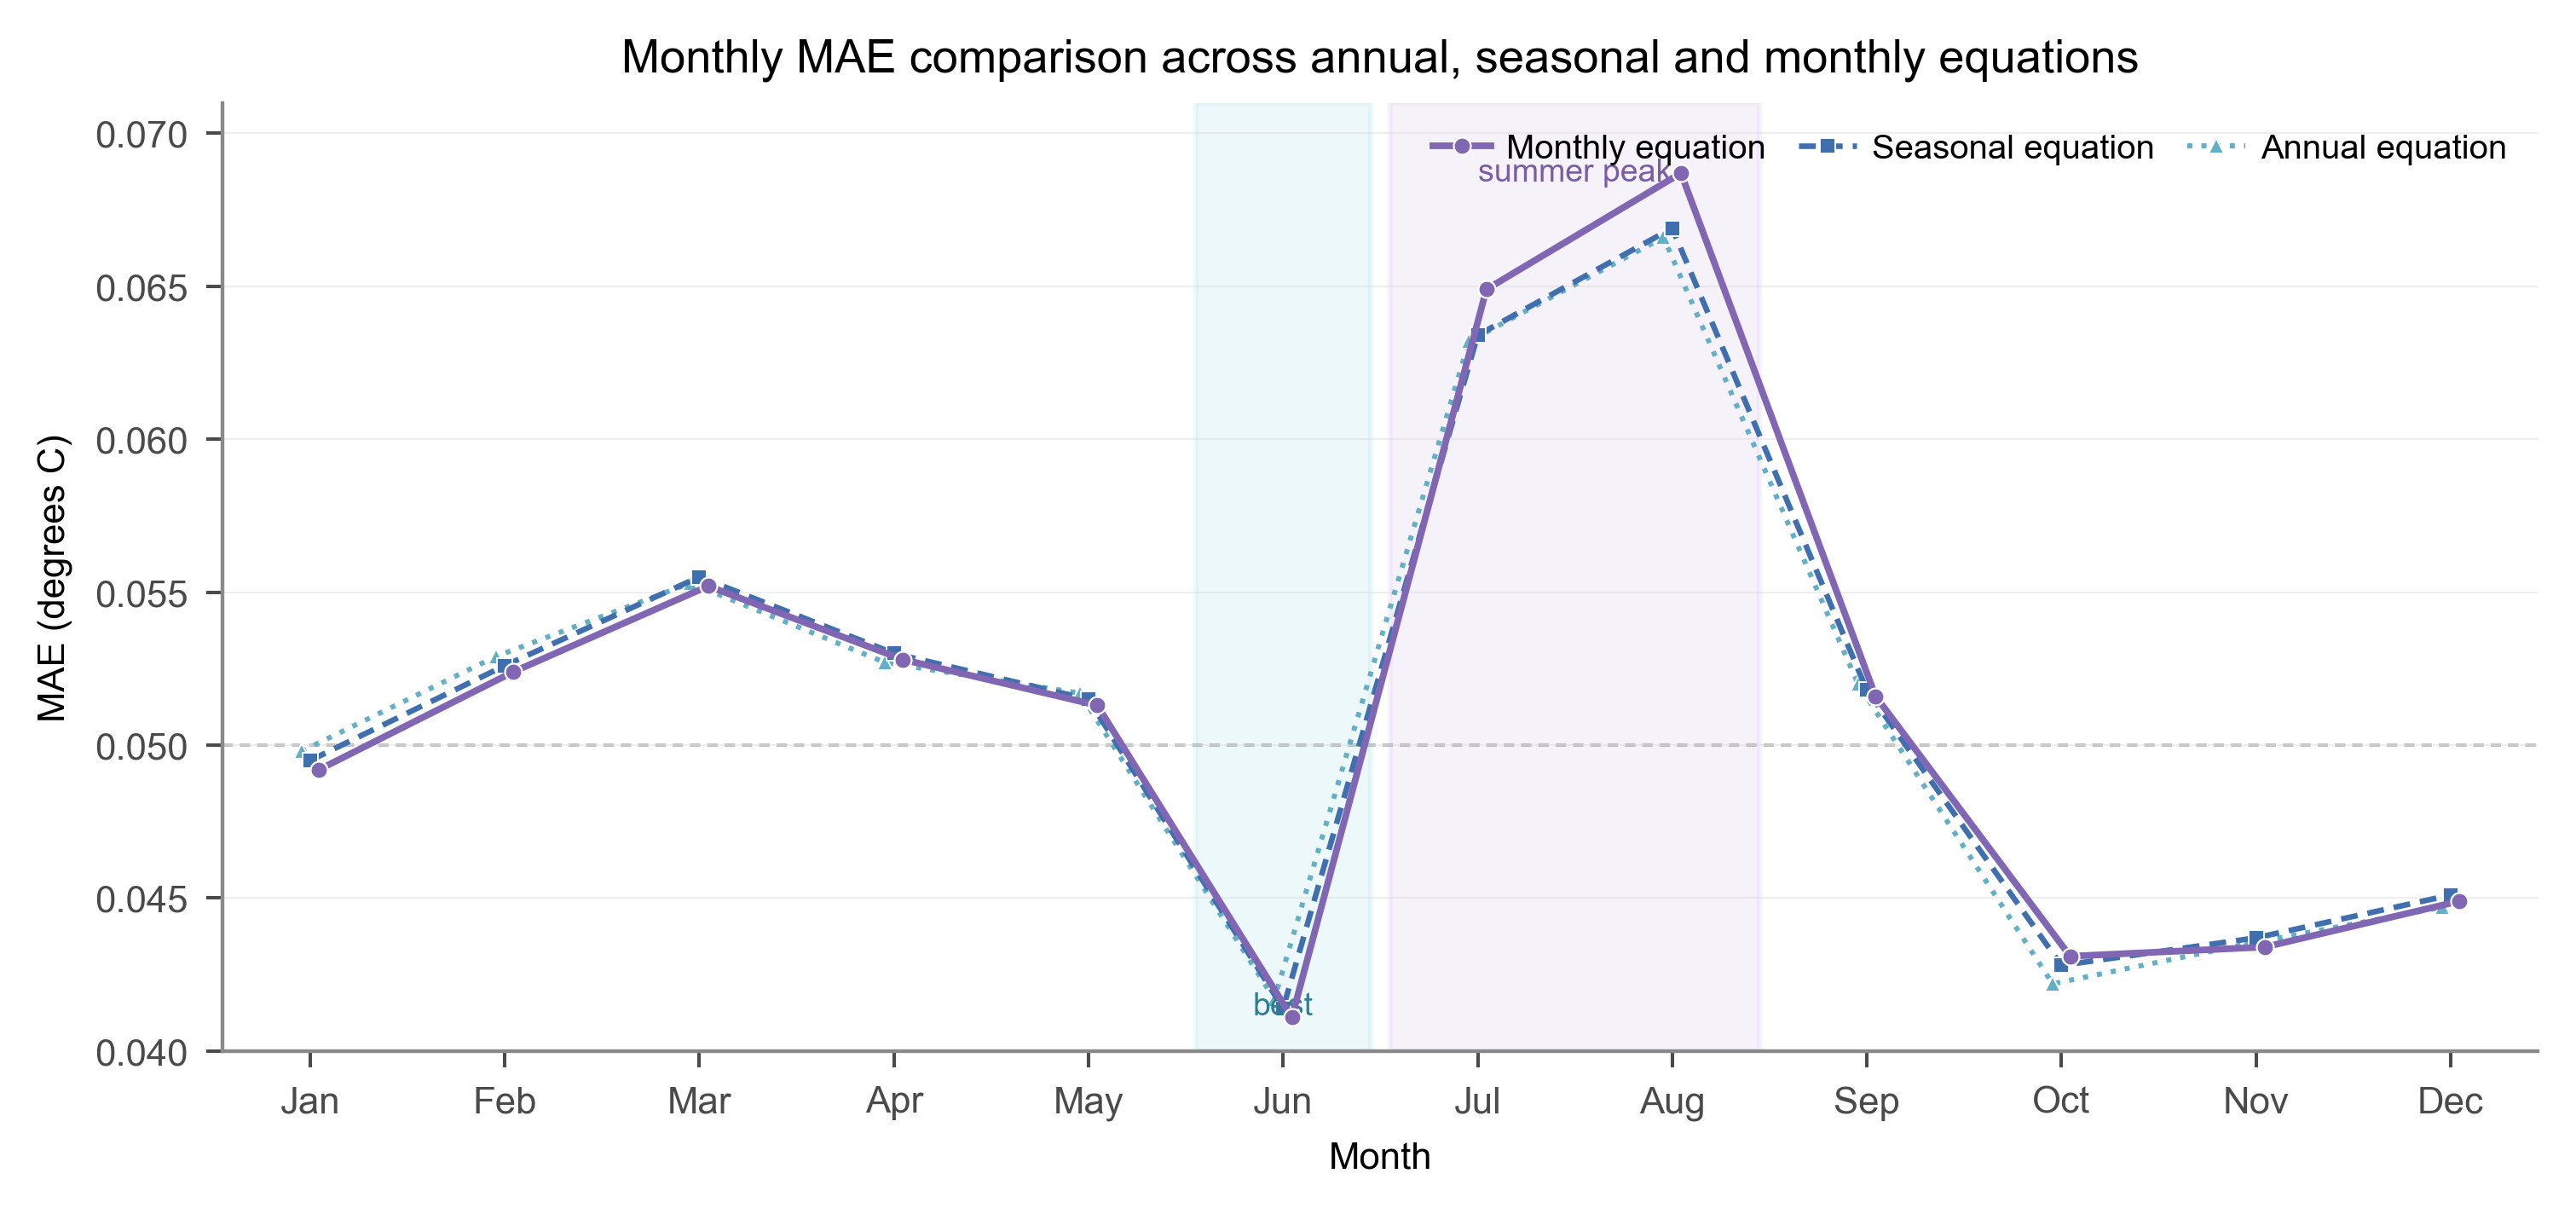
\includegraphics[width=0.96\linewidth]{../../results/figures/supporting/result2_monthly_mae_equation_comparison.png}
\caption{Monthly MAE comparison across annual, seasonal and monthly equation parameterizations for Result 2. The dashed reference line marks MAE = 0.05$^\circ$C, while the shaded intervals identify the June low-error month and the July--August summer peak.}
\label{fig:monthly-seasonal-annual-mae-comparison}
\end{figure}

\begin{table}[htbp]
\centering
\caption{Source table data corresponding to the monthly MAE comparison across monthly, seasonal and annual equations in Result 2.}
\label{tab:monthly-seasonal-annual-mae-values}
\small
\setlength{\tabcolsep}{4.5pt}
\renewcommand{\arraystretch}{1.10}
\begin{tabular}{C{1.0cm}C{1.0cm}ccc}
\toprule
Month & Season & Monthly model & Seasonal model & Annual model \\
\midrule
Jan & S1 & 0.0492 & 0.0495 & 0.0498 \\
Feb & S1 & 0.0524 & 0.0526 & 0.0529 \\
Mar & S1 & 0.0552 & 0.0555 & 0.0553 \\
Apr & S1 & 0.0528 & 0.0530 & 0.0527 \\
May & S1 & 0.0513 & 0.0515 & 0.0517 \\
Jun & S2 & 0.0411 & 0.0414 & 0.0417 \\
Jul & S2 & 0.0649 & 0.0634 & 0.0632 \\
Aug & S3 & 0.0687 & 0.0669 & 0.0666 \\
Sep & S3 & 0.0516 & 0.0518 & 0.0520 \\
Oct & S3 & 0.0431 & 0.0428 & 0.0422 \\
Nov & S4 & 0.0434 & 0.0437 & 0.0435 \\
Dec & S4 & 0.0449 & 0.0451 & 0.0447 \\
\bottomrule
\end{tabular}
\end{table}

\begin{table}[htbp]
\centering
\caption{Monthly Mixed-B coefficient records corresponding to the month-specific equation path. The coefficient columns follow the basis order $1$, $P$, $\ln P$, $\sqrt{P}$, $e^{-P/500}$, $e^{-P/1200}$, $(P+50)^{-1}$ and $(P+500)^{-1}$.}
\label{tab:monthly-mixedb-coefficient-records}
\scriptsize
\setlength{\tabcolsep}{2.4pt}
\renewcommand{\arraystretch}{1.08}
\resizebox{\textwidth}{!}{%
\begin{tabular}{llrrrrrrrrr}
\toprule
Month & Season & MAE & $c_0$ & $c_P$ & $c_{\ln P}$ & $c_{\sqrt{P}}$ & $c_{e500}$ & $c_{e1200}$ & $c_{50}^{-1}$ & $c_{500}^{-1}$ \\
\midrule
Jan & S1 & 0.0492 & 0.57433100 & -0.00070910 & 0.30951660 & 0.00332540 & 2.34111400 & 1.28270800 & 0.04045800 & 0.00534440 \\
Feb & S1 & 0.0524 & 0.57548300 & -0.00071256 & 0.31003500 & 0.00309500 & 2.35167400 & 1.28808400 & 0.04103400 & 0.00545000 \\
Mar & S1 & 0.0552 & 0.57682700 & -0.00071659 & 0.31063980 & 0.00282620 & 2.36399400 & 1.29435600 & 0.04170600 & 0.00557320 \\
Apr & S1 & 0.0528 & 0.57649100 & -0.00071558 & 0.31048860 & 0.00289340 & 2.36091400 & 1.29278800 & 0.04153800 & 0.00554240 \\
May & S1 & 0.0513 & 0.57668300 & -0.00071616 & 0.31057500 & 0.00285500 & 2.36267400 & 1.29368400 & 0.04163400 & 0.00556000 \\
Jun & S2 & 0.0411 & 0.59158700 & -0.00075200 & 0.31942400 & 0.00340600 & 2.29807400 & 1.28842500 & 0.04197600 & 0.00498300 \\
Jul & S2 & 0.0649 & 0.59758700 & -0.00077000 & 0.32212400 & 0.00220600 & 2.35307400 & 1.31642500 & 0.04497600 & 0.00553300 \\
Aug & S3 & 0.0687 & 0.54767500 & -0.00099438 & 0.30886175 & 0.01552800 & 2.14804950 & 1.22991900 & 0.01455750 & 0.00352388 \\
Sep & S3 & 0.0516 & 0.54422500 & -0.00098403 & 0.30730925 & 0.01621800 & 2.11642450 & 1.21381900 & 0.01283250 & 0.00320762 \\
Oct & S3 & 0.0431 & 0.53974000 & -0.00097058 & 0.30529100 & 0.01711500 & 2.07531200 & 1.19288900 & 0.01059000 & 0.00279650 \\
Nov & S4 & 0.0434 & 0.51693500 & -0.00101893 & 0.29714775 & 0.02081300 & 2.09310750 & 1.18374900 & 0.00148350 & 0.00269937 \\
Dec & S4 & 0.0449 & 0.52098500 & -0.00103108 & 0.29897025 & 0.02000300 & 2.13023250 & 1.20264900 & 0.00350850 & 0.00307063 \\
\bottomrule
\end{tabular}%
}
\end{table}

\noindent
The comparison shows that the monthly and seasonal parameterizations follow closely aligned MAE trajectories for most months, while the annual equation provides a stable single-parameter-set reference.
June forms the lowest-error month in this record, whereas July and August mark the summer error peak associated with stronger seasonal stratification.

\clearpage
% Auto-generated from corrected Result 2.4 daily prediction data.
\subsection{Daily Prediction Records for Result 2.4}
\label{subsec:result2-4-daily-prediction-records}

\noindent
This subsection records the day-by-day prediction-error source values for Result 2.4.
The sample-count column reports the corrected count after subtracting 10,000 from entries whose supplied count exceeded 10,000.
The corrected record spans 2025-01-01--2025-05-25, contains 145 daily entries and totals 1,354,997 samples.
The arithmetic mean daily MAE is 0.060607$^\circ$C and the sample-weighted mean MAE is 0.060774$^\circ$C.
The lowest daily MAE is 0.007079$^\circ$C on 2025-01-20, and the highest daily MAE is 0.102812$^\circ$C on 2025-05-15.

\begin{figure}[htbp]
\centering
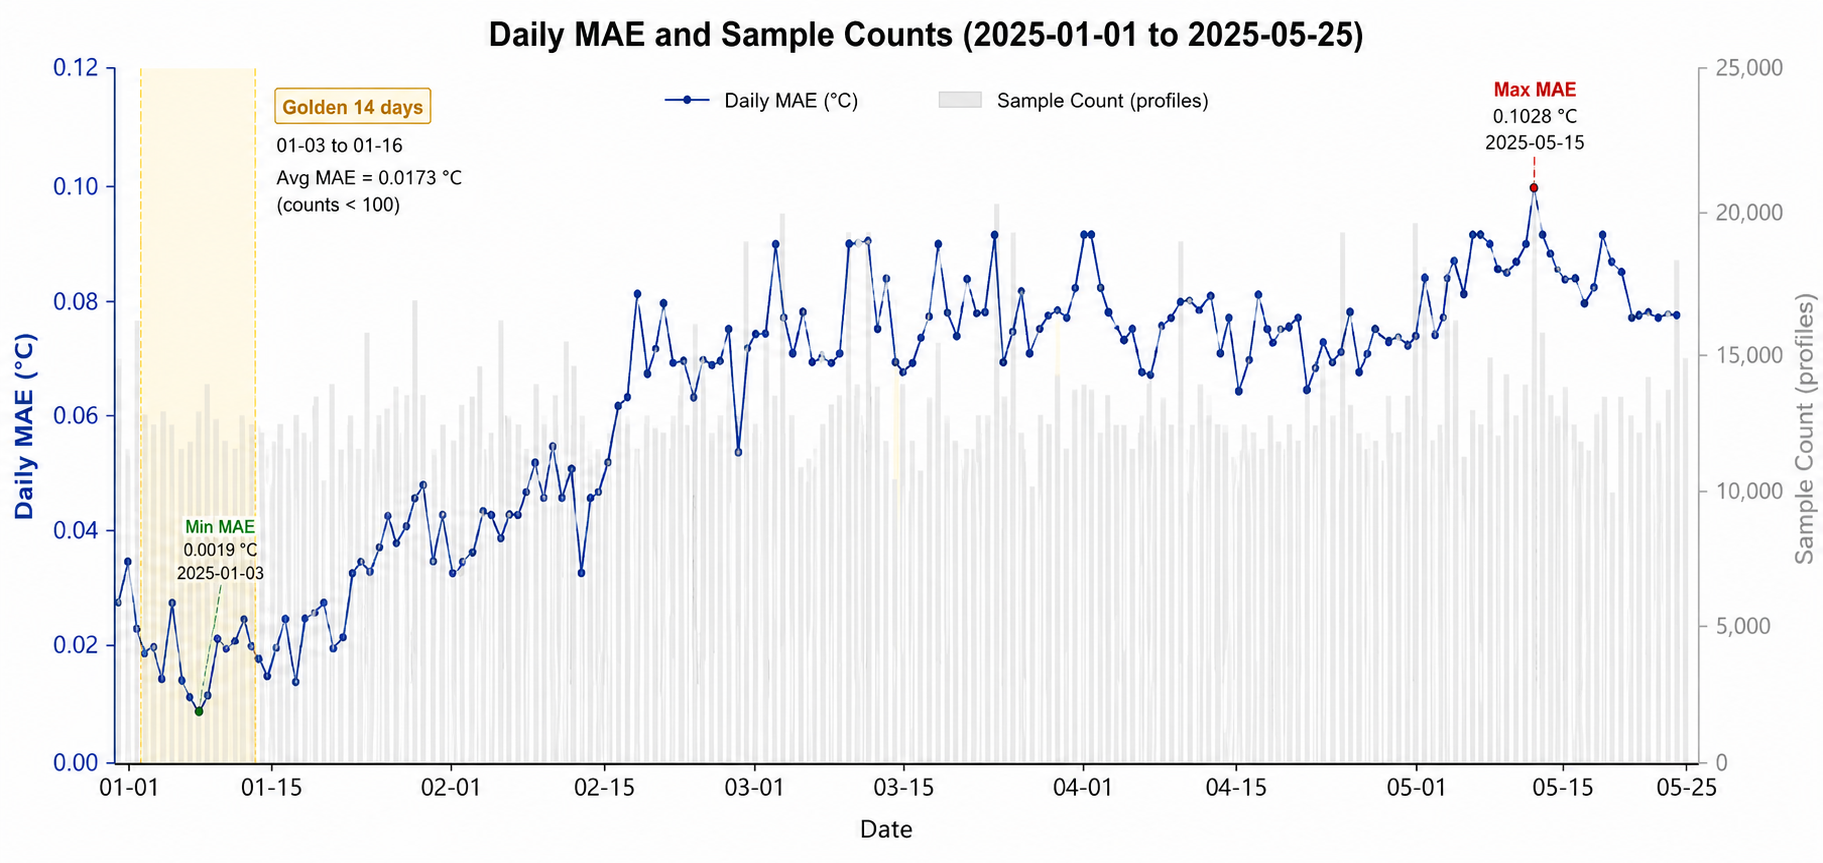
\includegraphics[width=0.98\linewidth]{../../results/figures/supporting/result2_4_daily_mae_sample_counts.png}
\caption{Daily MAE and sample-count visualization for the Result 2.4 prediction record from 2025-01-01 to 2025-05-25. The corrected tabular sample counts used for support-file lookup are reported in Tables~\ref{tab:result2-4-daily-prediction-monthly-summary} and \ref{tab:result2-4-daily-prediction-complete}.}
\label{fig:result2-4-daily-mae-sample-counts}
\end{figure}

\begin{table}[htbp]
\centering
\caption{Monthly summary of the corrected daily prediction records for Result 2.4. The weighted MAE uses the corrected daily sample counts.}
\label{tab:result2-4-daily-prediction-monthly-summary}
\small
\setlength{\tabcolsep}{4.6pt}
\renewcommand{\arraystretch}{1.08}
\begin{tabular}{lrrrrrr}
\toprule
Month & Days & Sample count & Mean MAE & Weighted MAE & Min MAE & Max MAE \\
\midrule
2025-01 & 31 & 287257 & 0.020521 & 0.020564 & 0.007079 & 0.035898 \\
2025-02 & 28 & 261991 & 0.047487 & 0.047492 & 0.019342 & 0.082274 \\
2025-03 & 31 & 288916 & 0.077832 & 0.078013 & 0.039598 & 0.100475 \\
2025-04 & 30 & 282145 & 0.073097 & 0.073136 & 0.056453 & 0.083768 \\
2025-05 & 25 & 234688 & 0.088658 & 0.088731 & 0.071020 & 0.102812 \\
\midrule
Total & 145 & 1354997 & 0.060607 & 0.060774 & 0.007079 & 0.102812 \\
\bottomrule
\end{tabular}
\end{table}

\begin{table}[htbp]
\centering
\caption{Complete corrected daily prediction source table for Result 2.4 in compact three-block layout. Each block lists date, MAE and corrected sample count.}
\label{tab:result2-4-daily-prediction-complete}
\scriptsize
\setlength{\tabcolsep}{3.2pt}
\renewcommand{\arraystretch}{0.88}
\resizebox{\textwidth}{!}{%
\begin{tabular}{lrrlrrlrr}
\toprule
Date & MAE & $n$ & Date & MAE & $n$ & Date & MAE & $n$ \\
\midrule
2025-01-01 & 0.018980 & 8694 & 2025-01-02 & 0.027031 & 9584 & 2025-01-03 & 0.009779 & 9170 \\
2025-01-04 & 0.012029 & 9600 & 2025-01-05 & 0.018997 & 9394 & 2025-01-06 & 0.017661 & 8369 \\
2025-01-07 & 0.021985 & 9564 & 2025-01-08 & 0.014047 & 9246 & 2025-01-09 & 0.022825 & 9565 \\
2025-01-10 & 0.012962 & 8835 & 2025-01-11 & 0.022851 & 8720 & 2025-01-12 & 0.019711 & 9537 \\
2025-01-13 & 0.015170 & 9032 & 2025-01-14 & 0.020290 & 9575 & 2025-01-15 & 0.014215 & 9209 \\
2025-01-16 & 0.020308 & 8844 & 2025-01-17 & 0.014368 & 9561 & 2025-01-18 & 0.019278 & 9199 \\
2025-01-19 & 0.025191 & 9550 & 2025-01-20 & 0.007079 & 9215 & 2025-01-21 & 0.024577 & 9004 \\
2025-01-22 & 0.021783 & 9549 & 2025-01-23 & 0.031040 & 9287 & 2025-01-24 & 0.022052 & 9582 \\
2025-01-25 & 0.026362 & 9399 & 2025-01-26 & 0.033309 & 8963 & 2025-01-27 & 0.035898 & 9578 \\
2025-01-28 & 0.019023 & 9461 & 2025-01-29 & 0.030743 & 9566 & 2025-01-30 & 0.016628 & 9466 \\
2025-01-31 & 0.019990 & 8939 & 2025-02-01 & 0.019342 & 9581 & 2025-02-02 & 0.030099 & 9429 \\
2025-02-03 & 0.026974 & 9539 & 2025-02-04 & 0.025222 & 9490 & 2025-02-05 & 0.031809 & 8948 \\
2025-02-06 & 0.030179 & 9581 & 2025-02-07 & 0.038389 & 9463 & 2025-02-08 & 0.030959 & 9537 \\
2025-02-09 & 0.041171 & 9435 & 2025-02-10 & 0.032850 & 8821 & 2025-02-11 & 0.038421 & 9551 \\
2025-02-12 & 0.019517 & 9180 & 2025-02-13 & 0.032697 & 9587 & 2025-02-14 & 0.031135 & 9265 \\
2025-02-15 & 0.039664 & 8975 & 2025-02-16 & 0.054980 & 9527 & 2025-02-17 & 0.056656 & 9352 \\
2025-02-18 & 0.082274 & 9578 & 2025-02-19 & 0.060704 & 9264 & 2025-02-20 & 0.070220 & 8711 \\
2025-02-21 & 0.080407 & 9556 & 2025-02-22 & 0.063748 & 9350 & 2025-02-23 & 0.068189 & 9565 \\
2025-02-24 & 0.055364 & 9337 & 2025-02-25 & 0.064026 & 8950 & 2025-02-26 & 0.064199 & 9527 \\
2025-02-27 & 0.064169 & 9303 & 2025-02-28 & 0.076265 & 9589 & 2025-03-01 & 0.039598 & 8773 \\
2025-03-02 & 0.068737 & 8974 & 2025-03-03 & 0.072830 & 9586 & 2025-03-04 & 0.067790 & 9230 \\
2025-03-05 & 0.094991 & 9515 & 2025-03-06 & 0.072224 & 9459 & 2025-03-07 & 0.072113 & 8822 \\
2025-03-08 & 0.077749 & 9589 & 2025-03-09 & 0.064917 & 9138 & 2025-03-10 & 0.064027 & 9536 \\
2025-03-11 & 0.065908 & 9187 & 2025-03-12 & 0.066929 & 8744 & 2025-03-13 & 0.091907 & 9552 \\
2025-03-14 & 0.093450 & 9484 & 2025-03-15 & 0.092467 & 9583 & 2025-03-16 & 0.064677 & 9138 \\
2025-03-17 & 0.100475 & 9031 & 2025-03-18 & 0.078064 & 9586 & 2025-03-19 & 0.087952 & 9267 \\
2025-03-20 & 0.093914 & 9548 & 2025-03-21 & 0.064053 & 9246 & 2025-03-22 & 0.082968 & 8905 \\
2025-03-23 & 0.072737 & 9588 & 2025-03-24 & 0.067365 & 9297 & 2025-03-25 & 0.075249 & 9567 \\
2025-03-26 & 0.074609 & 9443 & 2025-03-27 & 0.081439 & 9016 & 2025-03-28 & 0.090441 & 9575 \\
2025-03-29 & 0.080968 & 9476 & 2025-03-30 & 0.097658 & 9578 & 2025-03-31 & 0.094597 & 9483 \\
2025-04-01 & 0.080776 & 9034 & 2025-04-02 & 0.081737 & 9615 & 2025-04-03 & 0.075576 & 9464 \\
2025-04-04 & 0.075354 & 9543 & 2025-04-05 & 0.064313 & 9467 & 2025-04-06 & 0.060316 & 8912 \\
2025-04-07 & 0.077279 & 9615 & 2025-04-08 & 0.073870 & 9549 & 2025-04-09 & 0.080140 & 9561 \\
2025-04-10 & 0.081026 & 9511 & 2025-04-11 & 0.079554 & 9000 & 2025-04-12 & 0.083768 & 9570 \\
2025-04-13 & 0.064670 & 9474 & 2025-04-14 & 0.076561 & 9568 & 2025-04-15 & 0.056453 & 9148 \\
2025-04-16 & 0.073213 & 8951 & 2025-04-17 & 0.081870 & 9570 & 2025-04-18 & 0.068767 & 9384 \\
2025-04-19 & 0.080080 & 9561 & 2025-04-20 & 0.078762 & 9435 & 2025-04-21 & 0.071650 & 9009 \\
2025-04-22 & 0.072860 & 9577 & 2025-04-23 & 0.058648 & 9475 & 2025-04-24 & 0.067416 & 9574 \\
2025-04-25 & 0.065181 & 9466 & 2025-04-26 & 0.076377 & 9030 & 2025-04-27 & 0.078777 & 9560 \\
2025-04-28 & 0.062358 & 9464 & 2025-04-29 & 0.068339 & 9555 & 2025-04-30 & 0.077218 & 9503 \\
2025-05-01 & 0.075498 & 8837 & 2025-05-02 & 0.075541 & 9610 & 2025-05-03 & 0.071020 & 9377 \\
2025-05-04 & 0.086197 & 9565 & 2025-05-05 & 0.080553 & 9441 & 2025-05-06 & 0.076339 & 8818 \\
2025-05-07 & 0.093489 & 9584 & 2025-05-08 & 0.087121 & 9427 & 2025-05-09 & 0.099484 & 9577 \\
2025-05-10 & 0.102212 & 9470 & 2025-05-11 & 0.096702 & 9008 & 2025-05-12 & 0.090740 & 9509 \\
2025-05-13 & 0.095042 & 9437 & 2025-05-14 & 0.098386 & 9623 & 2025-05-15 & 0.102812 & 9479 \\
2025-05-16 & 0.089950 & 9006 & 2025-05-17 & 0.090370 & 9569 & 2025-05-18 & 0.090335 & 9461 \\
2025-05-19 & 0.087623 & 9578 & 2025-05-20 & 0.084832 & 9304 & 2025-05-21 & 0.087876 & 9019 \\
2025-05-22 & 0.095653 & 9580 & 2025-05-23 & 0.090977 & 9399 & 2025-05-24 & 0.090340 & 9562 \\
2025-05-25 & 0.077353 & 9448 &  &  &  &  &  &  \\
\bottomrule
\end{tabular}%
}
\end{table}

\clearpage
% Auto-generated from supporting_data/fixed_equation_daily_stability_2023_2024.csv.
\paragraph{Fixed-equation daily stability record for 2023--2024.}
The 2023--2024 fixed-equation daily stability record is compiled here as a companion daily evaluation record for the 2025 Result 2.4 prediction table.
It evaluates the fixed equation over the daily profile sets preceding the 2025 prediction window, so the 2023--2024 stability record and the 2025 prediction record are grouped under the same support-file subsection.
The record spans 2023-01-01--2024-12-31, contains 731 daily entries and totals 8,247,086 profile samples.
Across the complete record, the sample-weighted MAE is 0.048157$^\circ$C, the sample-weighted RMS RMSE is 0.090166$^\circ$C, and the day-mean $R^2$ is 0.993586.
All 731 daily entries satisfy the stability threshold MAE $\leq$ 0.10$^\circ$C and RMSE $\leq$ 0.20$^\circ$C.
The lowest daily MAE is 0.0292$^\circ$C on 2023-12-28, and the highest daily MAE is 0.0707$^\circ$C on 2023-05-15.

\begin{table}[htbp]
\centering
\caption{Annual summary of the fixed-equation daily stability evaluation record for 2023--2024.}
\label{tab:fixed-equation-daily-stability-annual}
\small
\setlength{\tabcolsep}{4.4pt}
\renewcommand{\arraystretch}{1.08}
\begin{tabular}{lrrrrrr}
\toprule
Year & Days & Sample count & Weighted MAE & RMS RMSE & Mean $R^2$ & Stable days \\
\midrule
2023 & 365 & 4083163 & 0.049001 & 0.091616 & 0.993471 & 365 \\
2024 & 366 & 4163923 & 0.047330 & 0.088721 & 0.993702 & 366 \\
\midrule
Total & 731 & 8247086 & 0.048157 & 0.090166 & 0.993586 & 731 \\
\bottomrule
\end{tabular}
\end{table}

\begin{table}[htbp]
\centering
\caption{Quarterly summary of sample density and fixed-equation stability metrics for 2023--2024.}
\label{tab:fixed-equation-daily-stability-quarterly}
\scriptsize
\setlength{\tabcolsep}{3.2pt}
\renewcommand{\arraystretch}{1.08}
\resizebox{\textwidth}{!}{%
\begin{tabular}{lrrrrrrr}
\toprule
Period & Days & Mean $n$ & Mean 1 m bins & Spacing (m) & Weighted MAE & RMS RMSE & Mean $R^2$ \\
\midrule
2023-Q1 & 90 & 11270 & 3665.9 & 1.0550 & 0.043390 & 0.084329 & 0.993976 \\
2023-Q2 & 91 & 11734 & 3688.8 & 1.0484 & 0.052655 & 0.095618 & 0.993192 \\
2023-Q3 & 92 & 11134 & 3605.8 & 1.0726 & 0.054728 & 0.099033 & 0.992876 \\
2023-Q4 & 92 & 10618 & 3583.7 & 1.0792 & 0.044826 & 0.086158 & 0.993848 \\
2024-Q1 & 91 & 11271 & 3653.1 & 1.0587 & 0.042038 & 0.078931 & 0.994280 \\
2024-Q2 & 91 & 11700 & 3632.9 & 1.0646 & 0.048210 & 0.090462 & 0.993681 \\
2024-Q3 & 92 & 11314 & 3536.1 & 1.0937 & 0.052959 & 0.097610 & 0.992926 \\
2024-Q4 & 92 & 11225 & 3669.0 & 1.0541 & 0.046004 & 0.086665 & 0.993925 \\
\bottomrule
\end{tabular}%
}
\end{table}

\begin{table}[htbp]
\centering
\caption{Segment-level summary of the fixed-equation daily stability evaluation record.}
\label{tab:fixed-equation-daily-stability-segment}
\small
\setlength{\tabcolsep}{4.2pt}
\renewcommand{\arraystretch}{1.08}
\begin{tabular}{lrrrrrr}
\toprule
Segment & Days & Sample count & Weighted MAE & RMS RMSE & Mean $R^2$ & Stable days \\
\midrule
2023 full year & 365 & 4083163 & 0.049001 & 0.091616 & 0.993471 & 365 \\
2024 H1 & 182 & 2090349 & 0.045182 & 0.085000 & 0.993981 & 182 \\
2024 Jul-Oct & 123 & 1388422 & 0.052470 & 0.096840 & 0.992983 & 123 \\
2024 Nov-Dec & 61 & 685152 & 0.043467 & 0.082408 & 0.994318 & 61 \\
\bottomrule
\end{tabular}
\end{table}

\begin{table}[htbp]
\centering
\caption{Monthly lookup summary for the fixed-equation daily stability evaluation record.}
\label{tab:fixed-equation-daily-stability-monthly}
\scriptsize
\setlength{\tabcolsep}{3.0pt}
\renewcommand{\arraystretch}{1.05}
\resizebox{\textwidth}{!}{%
\begin{tabular}{lrrrrrlrrrrr}
\toprule
Period & Days & Samples & W-MAE & RMS-RMSE & Mean $R^2$ & Period & Days & Samples & W-MAE & RMS-RMSE & Mean $R^2$ \\
\midrule
2023-01 & 31 & 341331 & 0.040675 & 0.080783 & 0.994029 & 2024-01 & 31 & 341403 & 0.039999 & 0.075295 & 0.994429 \\
2023-02 & 28 & 313223 & 0.043155 & 0.084122 & 0.994000 & 2024-02 & 29 & 326131 & 0.041806 & 0.078579 & 0.994134 \\
2023-03 & 31 & 359707 & 0.046172 & 0.087734 & 0.993900 & 2024-03 & 31 & 358110 & 0.044193 & 0.082553 & 0.994268 \\
2023-04 & 30 & 351343 & 0.049648 & 0.092237 & 0.993517 & 2024-04 & 30 & 349804 & 0.045998 & 0.086388 & 0.994130 \\
2023-05 & 31 & 365410 & 0.052660 & 0.096119 & 0.992958 & 2024-05 & 31 & 365943 & 0.048801 & 0.091513 & 0.993423 \\
2023-06 & 30 & 350997 & 0.055659 & 0.098380 & 0.993110 & 2024-06 & 30 & 348958 & 0.049808 & 0.093300 & 0.993500 \\
2023-07 & 31 & 353546 & 0.056661 & 0.100684 & 0.992581 & 2024-07 & 31 & 369818 & 0.051997 & 0.096368 & 0.993000 \\
2023-08 & 31 & 343963 & 0.055171 & 0.101114 & 0.992890 & 2024-08 & 31 & 328975 & 0.054008 & 0.099287 & 0.992981 \\
2023-09 & 30 & 326810 & 0.052169 & 0.094933 & 0.993167 & 2024-09 & 30 & 342095 & 0.052991 & 0.097316 & 0.992793 \\
2023-10 & 31 & 330004 & 0.048158 & 0.089689 & 0.993700 & 2024-10 & 31 & 347534 & 0.051005 & 0.094498 & 0.993152 \\
2023-11 & 30 & 316918 & 0.044656 & 0.085580 & 0.993913 & 2024-11 & 30 & 335165 & 0.045001 & 0.085292 & 0.993993 \\
2023-12 & 31 & 329911 & 0.041657 & 0.083051 & 0.993932 & 2024-12 & 31 & 349987 & 0.041997 & 0.079548 & 0.994632 \\
\bottomrule
\end{tabular}%
}
\end{table}

\clearpage
\begin{landscape}
\begingroup
\tiny
\setlength{\tabcolsep}{1.8pt}
\renewcommand{\arraystretch}{0.82}
\begin{longtable}{lrrrrlrrrrlrrrr}
\caption{Complete fixed-equation daily stability source table for 2023--2024 in compact three-block layout. Each block lists date, MAE, RMSE, $R^2$ and sample count.}\label{tab:fixed-equation-daily-stability-complete}\\
\toprule
Date & MAE & RMSE & $R^2$ & $n$ & Date & MAE & RMSE & $R^2$ & $n$ & Date & MAE & RMSE & $R^2$ & $n$ \\
\midrule
\endfirsthead
\caption[]{Complete fixed-equation daily stability source table for 2023--2024, continued.}\\
\toprule
Date & MAE & RMSE & $R^2$ & $n$ & Date & MAE & RMSE & $R^2$ & $n$ & Date & MAE & RMSE & $R^2$ & $n$ \\
\midrule
\endhead
\midrule
\multicolumn{15}{r}{Continued on next page}\\
\endfoot
\bottomrule
\endlastfoot
2023-01-01 & 0.0450 & 0.0773 & 0.9954 & 10959 & 2023-01-02 & 0.0433 & 0.0917 & 0.9927 & 10812 & 2023-01-03 & 0.0387 & 0.0919 & 0.9951 & 10549 \\
2023-01-04 & 0.0392 & 0.0793 & 0.9937 & 11109 & 2023-01-05 & 0.0327 & 0.0740 & 0.9939 & 10241 & 2023-01-06 & 0.0339 & 0.0792 & 0.9926 & 10556 \\
2023-01-07 & 0.0312 & 0.0656 & 0.9937 & 11781 & 2023-01-08 & 0.0346 & 0.0807 & 0.9934 & 11174 & 2023-01-09 & 0.0351 & 0.0689 & 0.9932 & 11349 \\
2023-01-10 & 0.0339 & 0.0713 & 0.9973 & 10696 & 2023-01-11 & 0.0352 & 0.0847 & 0.9945 & 11471 & 2023-01-12 & 0.0356 & 0.0845 & 0.9920 & 10619 \\
2023-01-13 & 0.0379 & 0.0792 & 0.9952 & 10386 & 2023-01-14 & 0.0396 & 0.0813 & 0.9938 & 11144 & 2023-01-15 & 0.0426 & 0.0712 & 0.9948 & 11371 \\
2023-01-16 & 0.0412 & 0.0791 & 0.9949 & 11370 & 2023-01-17 & 0.0367 & 0.0797 & 0.9933 & 11051 & 2023-01-18 & 0.0408 & 0.0691 & 0.9941 & 10335 \\
2023-01-19 & 0.0396 & 0.0798 & 0.9936 & 10157 & 2023-01-20 & 0.0369 & 0.0715 & 0.9945 & 11248 & 2023-01-21 & 0.0362 & 0.0852 & 0.9953 & 11029 \\
2023-01-22 & 0.0366 & 0.0727 & 0.9936 & 11254 & 2023-01-23 & 0.0377 & 0.0765 & 0.9955 & 11924 & 2023-01-24 & 0.0433 & 0.0849 & 0.9934 & 11308 \\
2023-01-25 & 0.0484 & 0.0856 & 0.9929 & 10650 & 2023-01-26 & 0.0522 & 0.0945 & 0.9944 & 11087 & 2023-01-27 & 0.0425 & 0.0767 & 0.9944 & 11094 \\
2023-01-28 & 0.0466 & 0.0873 & 0.9933 & 11715 & 2023-01-29 & 0.0543 & 0.0986 & 0.9940 & 10833 & 2023-01-30 & 0.0530 & 0.0767 & 0.9937 & 11435 \\
2023-01-31 & 0.0565 & 0.0949 & 0.9927 & 10624 & 2023-02-01 & 0.0388 & 0.0773 & 0.9949 & 11052 & 2023-02-02 & 0.0348 & 0.0829 & 0.9953 & 11041 \\
2023-02-03 & 0.0456 & 0.0835 & 0.9953 & 11008 & 2023-02-04 & 0.0412 & 0.0920 & 0.9942 & 11323 & 2023-02-05 & 0.0348 & 0.0863 & 0.9943 & 11322 \\
2023-02-06 & 0.0301 & 0.0596 & 0.9944 & 11282 & 2023-02-07 & 0.0364 & 0.0827 & 0.9952 & 11056 & 2023-02-08 & 0.0438 & 0.0824 & 0.9948 & 11420 \\
2023-02-09 & 0.0436 & 0.0800 & 0.9936 & 11380 & 2023-02-10 & 0.0472 & 0.0964 & 0.9943 & 10719 & 2023-02-11 & 0.0515 & 0.0893 & 0.9921 & 10731 \\
2023-02-12 & 0.0586 & 0.0958 & 0.9915 & 11050 & 2023-02-13 & 0.0516 & 0.0933 & 0.9942 & 10869 & 2023-02-14 & 0.0493 & 0.0899 & 0.9935 & 10387 \\
2023-02-15 & 0.0518 & 0.0892 & 0.9931 & 11022 & 2023-02-16 & 0.0473 & 0.0809 & 0.9953 & 10356 & 2023-02-17 & 0.0402 & 0.0781 & 0.9951 & 11560 \\
2023-02-18 & 0.0444 & 0.0828 & 0.9920 & 11438 & 2023-02-19 & 0.0449 & 0.0969 & 0.9937 & 10919 & 2023-02-20 & 0.0466 & 0.0979 & 0.9942 & 11364 \\
2023-02-21 & 0.0440 & 0.0793 & 0.9947 & 11264 & 2023-02-22 & 0.0457 & 0.0838 & 0.9937 & 11518 & 2023-02-23 & 0.0477 & 0.0783 & 0.9930 & 10991 \\
2023-02-24 & 0.0412 & 0.0804 & 0.9934 & 11332 & 2023-02-25 & 0.0353 & 0.0835 & 0.9930 & 11414 & 2023-02-26 & 0.0319 & 0.0636 & 0.9941 & 11588 \\
2023-02-27 & 0.0397 & 0.0866 & 0.9946 & 12095 & 2023-02-28 & 0.0431 & 0.0722 & 0.9945 & 11722 & 2023-03-01 & 0.0443 & 0.0820 & 0.9942 & 11318 \\
2023-03-02 & 0.0485 & 0.0892 & 0.9939 & 11637 & 2023-03-03 & 0.0512 & 0.0901 & 0.9943 & 11539 & 2023-03-04 & 0.0443 & 0.0923 & 0.9955 & 12008 \\
2023-03-05 & 0.0376 & 0.0699 & 0.9942 & 11479 & 2023-03-06 & 0.0424 & 0.0774 & 0.9940 & 11924 & 2023-03-07 & 0.0444 & 0.0926 & 0.9941 & 11122 \\
2023-03-08 & 0.0438 & 0.0827 & 0.9932 & 11588 & 2023-03-09 & 0.0430 & 0.0790 & 0.9940 & 12013 & 2023-03-10 & 0.0456 & 0.0939 & 0.9945 & 11463 \\
2023-03-11 & 0.0462 & 0.0889 & 0.9952 & 11437 & 2023-03-12 & 0.0476 & 0.0966 & 0.9944 & 11440 & 2023-03-13 & 0.0480 & 0.1005 & 0.9934 & 11616 \\
2023-03-14 & 0.0576 & 0.0851 & 0.9937 & 11786 & 2023-03-15 & 0.0521 & 0.0890 & 0.9938 & 12006 & 2023-03-16 & 0.0511 & 0.0935 & 0.9925 & 11281 \\
2023-03-17 & 0.0503 & 0.0897 & 0.9932 & 11502 & 2023-03-18 & 0.0485 & 0.0998 & 0.9943 & 11560 & 2023-03-19 & 0.0419 & 0.0769 & 0.9946 & 11666 \\
2023-03-20 & 0.0434 & 0.0821 & 0.9944 & 11174 & 2023-03-21 & 0.0398 & 0.0758 & 0.9951 & 11781 & 2023-03-22 & 0.0396 & 0.0867 & 0.9933 & 11395 \\
2023-03-23 & 0.0421 & 0.0794 & 0.9950 & 11639 & 2023-03-24 & 0.0460 & 0.0967 & 0.9933 & 11307 & 2023-03-25 & 0.0435 & 0.0828 & 0.9932 & 12364 \\
2023-03-26 & 0.0485 & 0.1015 & 0.9936 & 11526 & 2023-03-27 & 0.0523 & 0.0868 & 0.9910 & 12451 & 2023-03-28 & 0.0472 & 0.0879 & 0.9937 & 11651 \\
2023-03-29 & 0.0424 & 0.0766 & 0.9953 & 11590 & 2023-03-30 & 0.0502 & 0.0989 & 0.9929 & 10977 & 2023-03-31 & 0.0477 & 0.0862 & 0.9931 & 11467 \\
2023-04-01 & 0.0524 & 0.0816 & 0.9922 & 12406 & 2023-04-02 & 0.0436 & 0.0765 & 0.9940 & 11728 & 2023-04-03 & 0.0453 & 0.0900 & 0.9949 & 11115 \\
2023-04-04 & 0.0544 & 0.0886 & 0.9940 & 10533 & 2023-04-05 & 0.0520 & 0.0930 & 0.9938 & 11233 & 2023-04-06 & 0.0524 & 0.1023 & 0.9944 & 11489 \\
2023-04-07 & 0.0509 & 0.0923 & 0.9940 & 10981 & 2023-04-08 & 0.0442 & 0.0963 & 0.9952 & 11521 & 2023-04-09 & 0.0555 & 0.0995 & 0.9934 & 11464 \\
2023-04-10 & 0.0486 & 0.0864 & 0.9932 & 11751 & 2023-04-11 & 0.0498 & 0.0868 & 0.9937 & 12167 & 2023-04-12 & 0.0520 & 0.1052 & 0.9935 & 11619 \\
2023-04-13 & 0.0469 & 0.0939 & 0.9952 & 11783 & 2023-04-14 & 0.0543 & 0.0984 & 0.9907 & 11698 & 2023-04-15 & 0.0507 & 0.0981 & 0.9924 & 11941 \\
2023-04-16 & 0.0536 & 0.1052 & 0.9927 & 12073 & 2023-04-17 & 0.0564 & 0.0951 & 0.9926 & 11475 & 2023-04-18 & 0.0540 & 0.0917 & 0.9932 & 12785 \\
2023-04-19 & 0.0557 & 0.0982 & 0.9927 & 11593 & 2023-04-20 & 0.0526 & 0.1022 & 0.9930 & 11970 & 2023-04-21 & 0.0465 & 0.0874 & 0.9954 & 11263 \\
2023-04-22 & 0.0434 & 0.0945 & 0.9922 & 12323 & 2023-04-23 & 0.0467 & 0.0894 & 0.9935 & 12661 & 2023-04-24 & 0.0497 & 0.0897 & 0.9926 & 11821 \\
2023-04-25 & 0.0500 & 0.0904 & 0.9921 & 11648 & 2023-04-26 & 0.0503 & 0.0890 & 0.9948 & 11165 & 2023-04-27 & 0.0498 & 0.0930 & 0.9940 & 11749 \\
2023-04-28 & 0.0444 & 0.0796 & 0.9932 & 11125 & 2023-04-29 & 0.0432 & 0.0855 & 0.9952 & 12583 & 2023-04-30 & 0.0408 & 0.0785 & 0.9937 & 11680 \\
2023-05-01 & 0.0524 & 0.1009 & 0.9921 & 12326 & 2023-05-02 & 0.0499 & 0.0953 & 0.9945 & 12018 & 2023-05-03 & 0.0494 & 0.0959 & 0.9928 & 11620 \\
2023-05-04 & 0.0557 & 0.0902 & 0.9935 & 12032 & 2023-05-05 & 0.0531 & 0.0889 & 0.9929 & 12348 & 2023-05-06 & 0.0487 & 0.0951 & 0.9926 & 12021 \\
2023-05-07 & 0.0518 & 0.0960 & 0.9921 & 11677 & 2023-05-08 & 0.0544 & 0.0982 & 0.9928 & 11495 & 2023-05-09 & 0.0503 & 0.0912 & 0.9923 & 12174 \\
2023-05-10 & 0.0572 & 0.1075 & 0.9932 & 11479 & 2023-05-11 & 0.0530 & 0.1035 & 0.9936 & 12073 & 2023-05-12 & 0.0555 & 0.0912 & 0.9938 & 12067 \\
2023-05-13 & 0.0605 & 0.1050 & 0.9923 & 11616 & 2023-05-14 & 0.0640 & 0.1068 & 0.9909 & 11686 & 2023-05-15 & 0.0707 & 0.1137 & 0.9911 & 12221 \\
2023-05-16 & 0.0552 & 0.1007 & 0.9921 & 11955 & 2023-05-17 & 0.0575 & 0.0990 & 0.9935 & 11351 & 2023-05-18 & 0.0548 & 0.0929 & 0.9931 & 11497 \\
2023-05-19 & 0.0521 & 0.1048 & 0.9925 & 12603 & 2023-05-20 & 0.0465 & 0.1036 & 0.9931 & 11132 & 2023-05-21 & 0.0466 & 0.0805 & 0.9940 & 11479 \\
2023-05-22 & 0.0455 & 0.0852 & 0.9941 & 10971 & 2023-05-23 & 0.0518 & 0.0910 & 0.9930 & 11340 & 2023-05-24 & 0.0549 & 0.1056 & 0.9930 & 11568 \\
2023-05-25 & 0.0542 & 0.0965 & 0.9922 & 11891 & 2023-05-26 & 0.0503 & 0.0935 & 0.9931 & 11517 & 2023-05-27 & 0.0505 & 0.0849 & 0.9914 & 11005 \\
2023-05-28 & 0.0445 & 0.0937 & 0.9943 & 12175 & 2023-05-29 & 0.0443 & 0.0904 & 0.9952 & 11980 & 2023-05-30 & 0.0483 & 0.0814 & 0.9935 & 12457 \\
2023-05-31 & 0.0482 & 0.0851 & 0.9931 & 11636 & 2023-06-01 & 0.0559 & 0.0959 & 0.9915 & 10858 & 2023-06-02 & 0.0606 & 0.1080 & 0.9921 & 11143 \\
2023-06-03 & 0.0569 & 0.1018 & 0.9937 & 11672 & 2023-06-04 & 0.0524 & 0.0890 & 0.9944 & 10650 & 2023-06-05 & 0.0465 & 0.0857 & 0.9965 & 11867 \\
2023-06-06 & 0.0451 & 0.0957 & 0.9946 & 12233 & 2023-06-07 & 0.0505 & 0.0992 & 0.9920 & 12424 & 2023-06-08 & 0.0512 & 0.1003 & 0.9922 & 11601 \\
2023-06-09 & 0.0526 & 0.1030 & 0.9942 & 11893 & 2023-06-10 & 0.0564 & 0.0856 & 0.9925 & 11870 & 2023-06-11 & 0.0578 & 0.1026 & 0.9943 & 11372 \\
2023-06-12 & 0.0665 & 0.1100 & 0.9922 & 11740 & 2023-06-13 & 0.0656 & 0.1035 & 0.9911 & 12499 & 2023-06-14 & 0.0670 & 0.1136 & 0.9915 & 11575 \\
2023-06-15 & 0.0659 & 0.0937 & 0.9917 & 12138 & 2023-06-16 & 0.0595 & 0.1033 & 0.9920 & 12464 & 2023-06-17 & 0.0606 & 0.1014 & 0.9936 & 11170 \\
2023-06-18 & 0.0596 & 0.1063 & 0.9941 & 11798 & 2023-06-19 & 0.0594 & 0.1096 & 0.9928 & 12112 & 2023-06-20 & 0.0584 & 0.1071 & 0.9927 & 11234 \\
2023-06-21 & 0.0578 & 0.1040 & 0.9935 & 11509 & 2023-06-22 & 0.0480 & 0.1030 & 0.9943 & 11490 & 2023-06-23 & 0.0487 & 0.0977 & 0.9941 & 11979 \\
2023-06-24 & 0.0539 & 0.0838 & 0.9926 & 12232 & 2023-06-25 & 0.0483 & 0.0834 & 0.9922 & 11548 & 2023-06-26 & 0.0500 & 0.0886 & 0.9935 & 11657 \\
2023-06-27 & 0.0475 & 0.0900 & 0.9929 & 11786 & 2023-06-28 & 0.0582 & 0.0878 & 0.9930 & 11323 & 2023-06-29 & 0.0532 & 0.0928 & 0.9940 & 11970 \\
2023-06-30 & 0.0559 & 0.0942 & 0.9935 & 11190 & 2023-07-01 & 0.0625 & 0.0975 & 0.9931 & 11262 & 2023-07-02 & 0.0629 & 0.0985 & 0.9916 & 11256 \\
2023-07-03 & 0.0663 & 0.1081 & 0.9910 & 11016 & 2023-07-04 & 0.0641 & 0.1055 & 0.9939 & 12125 & 2023-07-05 & 0.0603 & 0.1038 & 0.9935 & 11646 \\
2023-07-06 & 0.0560 & 0.1018 & 0.9934 & 11972 & 2023-07-07 & 0.0584 & 0.1101 & 0.9915 & 11838 & 2023-07-08 & 0.0541 & 0.0898 & 0.9915 & 10955 \\
2023-07-09 & 0.0486 & 0.1007 & 0.9940 & 11378 & 2023-07-10 & 0.0591 & 0.0981 & 0.9922 & 11466 & 2023-07-11 & 0.0538 & 0.0987 & 0.9905 & 11198 \\
2023-07-12 & 0.0589 & 0.1045 & 0.9928 & 12051 & 2023-07-13 & 0.0479 & 0.0985 & 0.9939 & 11335 & 2023-07-14 & 0.0522 & 0.0885 & 0.9914 & 11800 \\
2023-07-15 & 0.0642 & 0.0973 & 0.9903 & 11150 & 2023-07-16 & 0.0547 & 0.1026 & 0.9928 & 11340 & 2023-07-17 & 0.0516 & 0.1012 & 0.9936 & 11989 \\
2023-07-18 & 0.0538 & 0.0957 & 0.9945 & 11377 & 2023-07-19 & 0.0549 & 0.1060 & 0.9924 & 10103 & 2023-07-20 & 0.0623 & 0.0987 & 0.9915 & 11392 \\
2023-07-21 & 0.0612 & 0.1012 & 0.9938 & 11727 & 2023-07-22 & 0.0680 & 0.1005 & 0.9895 & 10801 & 2023-07-23 & 0.0610 & 0.1065 & 0.9919 & 11938 \\
2023-07-24 & 0.0568 & 0.1060 & 0.9929 & 11745 & 2023-07-25 & 0.0507 & 0.0936 & 0.9922 & 12099 & 2023-07-26 & 0.0493 & 0.0968 & 0.9935 & 10765 \\
2023-07-27 & 0.0466 & 0.0991 & 0.9943 & 11380 & 2023-07-28 & 0.0467 & 0.1049 & 0.9937 & 10934 & 2023-07-29 & 0.0562 & 0.1019 & 0.9933 & 11166 \\
2023-07-30 & 0.0539 & 0.0970 & 0.9932 & 11443 & 2023-07-31 & 0.0593 & 0.1042 & 0.9923 & 10899 & 2023-08-01 & 0.0594 & 0.1024 & 0.9924 & 11734 \\
2023-08-02 & 0.0617 & 0.1101 & 0.9929 & 11146 & 2023-08-03 & 0.0588 & 0.1045 & 0.9939 & 11200 & 2023-08-04 & 0.0558 & 0.1018 & 0.9929 & 10854 \\
2023-08-05 & 0.0578 & 0.0957 & 0.9928 & 11023 & 2023-08-06 & 0.0529 & 0.0979 & 0.9932 & 11747 & 2023-08-07 & 0.0547 & 0.1047 & 0.9934 & 11076 \\
2023-08-08 & 0.0580 & 0.1056 & 0.9917 & 10957 & 2023-08-09 & 0.0623 & 0.1118 & 0.9925 & 11498 & 2023-08-10 & 0.0527 & 0.1058 & 0.9947 & 10961 \\
2023-08-11 & 0.0426 & 0.0831 & 0.9935 & 11592 & 2023-08-12 & 0.0413 & 0.0996 & 0.9934 & 10811 & 2023-08-13 & 0.0466 & 0.0918 & 0.9943 & 11430 \\
2023-08-14 & 0.0491 & 0.0999 & 0.9921 & 10631 & 2023-08-15 & 0.0554 & 0.1019 & 0.9936 & 11392 & 2023-08-16 & 0.0536 & 0.1006 & 0.9936 & 10824 \\
2023-08-17 & 0.0562 & 0.1088 & 0.9925 & 11864 & 2023-08-18 & 0.0517 & 0.0844 & 0.9932 & 11236 & 2023-08-19 & 0.0553 & 0.1057 & 0.9936 & 10971 \\
2023-08-20 & 0.0597 & 0.0919 & 0.9908 & 11597 & 2023-08-21 & 0.0552 & 0.1008 & 0.9929 & 10777 & 2023-08-22 & 0.0572 & 0.0944 & 0.9914 & 10882 \\
2023-08-23 & 0.0582 & 0.1095 & 0.9908 & 10921 & 2023-08-24 & 0.0524 & 0.1006 & 0.9940 & 11505 & 2023-08-25 & 0.0490 & 0.0870 & 0.9933 & 10209 \\
2023-08-26 & 0.0513 & 0.1043 & 0.9930 & 10654 & 2023-08-27 & 0.0577 & 0.0855 & 0.9927 & 11383 & 2023-08-28 & 0.0581 & 0.1048 & 0.9913 & 11397 \\
2023-08-29 & 0.0586 & 0.1102 & 0.9924 & 10622 & 2023-08-30 & 0.0684 & 0.1149 & 0.9928 & 10655 & 2023-08-31 & 0.0584 & 0.1058 & 0.9940 & 10414 \\
2023-09-01 & 0.0543 & 0.0952 & 0.9923 & 11008 & 2023-09-02 & 0.0539 & 0.0861 & 0.9924 & 10379 & 2023-09-03 & 0.0491 & 0.0786 & 0.9932 & 10880 \\
2023-09-04 & 0.0488 & 0.0825 & 0.9925 & 10497 & 2023-09-05 & 0.0494 & 0.0841 & 0.9933 & 11198 & 2023-09-06 & 0.0509 & 0.0977 & 0.9932 & 10596 \\
2023-09-07 & 0.0539 & 0.0968 & 0.9935 & 10410 & 2023-09-08 & 0.0542 & 0.1011 & 0.9944 & 10802 & 2023-09-09 & 0.0388 & 0.0863 & 0.9953 & 10990 \\
2023-09-10 & 0.0395 & 0.0863 & 0.9936 & 11057 & 2023-09-11 & 0.0488 & 0.1002 & 0.9919 & 10927 & 2023-09-12 & 0.0444 & 0.0876 & 0.9957 & 10694 \\
2023-09-13 & 0.0436 & 0.0864 & 0.9958 & 11320 & 2023-09-14 & 0.0504 & 0.0828 & 0.9923 & 11471 & 2023-09-15 & 0.0509 & 0.0922 & 0.9943 & 10697 \\
2023-09-16 & 0.0542 & 0.1025 & 0.9923 & 10603 & 2023-09-17 & 0.0572 & 0.1078 & 0.9928 & 10856 & 2023-09-18 & 0.0595 & 0.1105 & 0.9934 & 11065 \\
2023-09-19 & 0.0567 & 0.1004 & 0.9919 & 12066 & 2023-09-20 & 0.0557 & 0.1083 & 0.9946 & 10693 & 2023-09-21 & 0.0565 & 0.0979 & 0.9929 & 10250 \\
2023-09-22 & 0.0569 & 0.0873 & 0.9921 & 11336 & 2023-09-23 & 0.0550 & 0.1065 & 0.9930 & 11667 & 2023-09-24 & 0.0629 & 0.0925 & 0.9911 & 10775 \\
2023-09-25 & 0.0534 & 0.0980 & 0.9934 & 10529 & 2023-09-26 & 0.0536 & 0.0937 & 0.9922 & 11315 & 2023-09-27 & 0.0582 & 0.0973 & 0.9930 & 10351 \\
2023-09-28 & 0.0528 & 0.1000 & 0.9932 & 10498 & 2023-09-29 & 0.0477 & 0.0892 & 0.9931 & 10661 & 2023-09-30 & 0.0542 & 0.1010 & 0.9923 & 11219 \\
2023-10-01 & 0.0552 & 0.0939 & 0.9952 & 10869 & 2023-10-02 & 0.0524 & 0.0865 & 0.9926 & 10501 & 2023-10-03 & 0.0503 & 0.0896 & 0.9929 & 10745 \\
2023-10-04 & 0.0559 & 0.0982 & 0.9916 & 11152 & 2023-10-05 & 0.0506 & 0.0810 & 0.9937 & 10394 & 2023-10-06 & 0.0532 & 0.1049 & 0.9917 & 10498 \\
2023-10-07 & 0.0484 & 0.0926 & 0.9932 & 10384 & 2023-10-08 & 0.0511 & 0.0860 & 0.9927 & 10539 & 2023-10-09 & 0.0510 & 0.0966 & 0.9953 & 10500 \\
2023-10-10 & 0.0455 & 0.0792 & 0.9939 & 10582 & 2023-10-11 & 0.0388 & 0.0821 & 0.9936 & 10929 & 2023-10-12 & 0.0369 & 0.0800 & 0.9963 & 10931 \\
2023-10-13 & 0.0446 & 0.0960 & 0.9953 & 10088 & 2023-10-14 & 0.0363 & 0.0886 & 0.9949 & 10234 & 2023-10-15 & 0.0467 & 0.0874 & 0.9937 & 10127 \\
2023-10-16 & 0.0438 & 0.0904 & 0.9936 & 11203 & 2023-10-17 & 0.0438 & 0.0805 & 0.9933 & 10287 & 2023-10-18 & 0.0471 & 0.0909 & 0.9948 & 10505 \\
2023-10-19 & 0.0444 & 0.0827 & 0.9945 & 10880 & 2023-10-20 & 0.0488 & 0.0899 & 0.9935 & 10055 & 2023-10-21 & 0.0465 & 0.0847 & 0.9959 & 10850 \\
2023-10-22 & 0.0469 & 0.0860 & 0.9947 & 11268 & 2023-10-23 & 0.0518 & 0.1011 & 0.9922 & 10398 & 2023-10-24 & 0.0516 & 0.1030 & 0.9931 & 10911 \\
2023-10-25 & 0.0536 & 0.0877 & 0.9928 & 10134 & 2023-10-26 & 0.0590 & 0.0957 & 0.9925 & 10123 & 2023-10-27 & 0.0533 & 0.0998 & 0.9922 & 11494 \\
2023-10-28 & 0.0472 & 0.0923 & 0.9946 & 10469 & 2023-10-29 & 0.0470 & 0.0781 & 0.9928 & 11210 & 2023-10-30 & 0.0477 & 0.0857 & 0.9929 & 10796 \\
2023-10-31 & 0.0439 & 0.0806 & 0.9947 & 10948 & 2023-11-01 & 0.0460 & 0.0906 & 0.9943 & 10965 & 2023-11-02 & 0.0498 & 0.0852 & 0.9932 & 9934 \\
2023-11-03 & 0.0422 & 0.0858 & 0.9930 & 10738 & 2023-11-04 & 0.0372 & 0.0668 & 0.9937 & 11155 & 2023-11-05 & 0.0372 & 0.0787 & 0.9943 & 10112 \\
2023-11-06 & 0.0480 & 0.0903 & 0.9951 & 11392 & 2023-11-07 & 0.0479 & 0.0733 & 0.9934 & 10200 & 2023-11-08 & 0.0445 & 0.0705 & 0.9940 & 10490 \\
2023-11-09 & 0.0452 & 0.0879 & 0.9927 & 9880 & 2023-11-10 & 0.0426 & 0.0792 & 0.9939 & 10294 & 2023-11-11 & 0.0325 & 0.0759 & 0.9962 & 10055 \\
2023-11-12 & 0.0392 & 0.0766 & 0.9953 & 9828 & 2023-11-13 & 0.0480 & 0.0914 & 0.9950 & 10593 & 2023-11-14 & 0.0551 & 0.0939 & 0.9920 & 10303 \\
2023-11-15 & 0.0492 & 0.1015 & 0.9941 & 11480 & 2023-11-16 & 0.0479 & 0.0977 & 0.9921 & 10457 & 2023-11-17 & 0.0541 & 0.0913 & 0.9937 & 11253 \\
2023-11-18 & 0.0508 & 0.0936 & 0.9932 & 11084 & 2023-11-19 & 0.0501 & 0.1017 & 0.9913 & 9958 & 2023-11-20 & 0.0477 & 0.0854 & 0.9942 & 10342 \\
2023-11-21 & 0.0478 & 0.0842 & 0.9936 & 11252 & 2023-11-22 & 0.0375 & 0.0874 & 0.9960 & 10247 & 2023-11-23 & 0.0435 & 0.0863 & 0.9931 & 10101 \\
2023-11-24 & 0.0402 & 0.0920 & 0.9929 & 10551 & 2023-11-25 & 0.0395 & 0.0880 & 0.9945 & 10412 & 2023-11-26 & 0.0417 & 0.0824 & 0.9947 & 10843 \\
2023-11-27 & 0.0455 & 0.0720 & 0.9937 & 10529 & 2023-11-28 & 0.0426 & 0.0822 & 0.9934 & 10837 & 2023-11-29 & 0.0435 & 0.0885 & 0.9954 & 10796 \\
2023-11-30 & 0.0410 & 0.0714 & 0.9954 & 10837 & 2023-12-01 & 0.0409 & 0.0681 & 0.9937 & 10344 & 2023-12-02 & 0.0405 & 0.0829 & 0.9945 & 11192 \\
2023-12-03 & 0.0492 & 0.0929 & 0.9943 & 10986 & 2023-12-04 & 0.0506 & 0.0987 & 0.9935 & 10520 & 2023-12-05 & 0.0451 & 0.0754 & 0.9930 & 10125 \\
2023-12-06 & 0.0438 & 0.0921 & 0.9931 & 10910 & 2023-12-07 & 0.0449 & 0.0767 & 0.9936 & 11243 & 2023-12-08 & 0.0401 & 0.0925 & 0.9939 & 10258 \\
2023-12-09 & 0.0473 & 0.0988 & 0.9929 & 9899 & 2023-12-10 & 0.0415 & 0.0941 & 0.9948 & 11308 & 2023-12-11 & 0.0436 & 0.0835 & 0.9932 & 10554 \\
2023-12-12 & 0.0430 & 0.0744 & 0.9937 & 11029 & 2023-12-13 & 0.0422 & 0.0794 & 0.9937 & 10585 & 2023-12-14 & 0.0407 & 0.0795 & 0.9947 & 10886 \\
2023-12-15 & 0.0409 & 0.0908 & 0.9950 & 10056 & 2023-12-16 & 0.0459 & 0.0894 & 0.9927 & 10351 & 2023-12-17 & 0.0491 & 0.0902 & 0.9930 & 11225 \\
2023-12-18 & 0.0432 & 0.0924 & 0.9927 & 11145 & 2023-12-19 & 0.0412 & 0.0748 & 0.9943 & 9989 & 2023-12-20 & 0.0392 & 0.0667 & 0.9921 & 10694 \\
2023-12-21 & 0.0477 & 0.0914 & 0.9944 & 10567 & 2023-12-22 & 0.0375 & 0.0786 & 0.9941 & 10386 & 2023-12-23 & 0.0423 & 0.0735 & 0.9942 & 10709 \\
2023-12-24 & 0.0459 & 0.0917 & 0.9951 & 11197 & 2023-12-25 & 0.0354 & 0.0857 & 0.9951 & 9773 & 2023-12-26 & 0.0320 & 0.0716 & 0.9947 & 10939 \\
2023-12-27 & 0.0294 & 0.0635 & 0.9943 & 10730 & 2023-12-28 & 0.0292 & 0.0727 & 0.9952 & 10523 & 2023-12-29 & 0.0391 & 0.0880 & 0.9942 & 11424 \\
2023-12-30 & 0.0414 & 0.0734 & 0.9952 & 10028 & 2023-12-31 & 0.0378 & 0.0717 & 0.9930 & 10336 & 2024-01-01 & 0.0394 & 0.0801 & 0.9944 & 10558 \\
2024-01-02 & 0.0334 & 0.0683 & 0.9961 & 11321 & 2024-01-03 & 0.0358 & 0.0659 & 0.9939 & 11106 & 2024-01-04 & 0.0362 & 0.0769 & 0.9939 & 10380 \\
2024-01-05 & 0.0374 & 0.0647 & 0.9945 & 10403 & 2024-01-06 & 0.0493 & 0.0776 & 0.9938 & 11335 & 2024-01-07 & 0.0460 & 0.0761 & 0.9928 & 10856 \\
2024-01-08 & 0.0464 & 0.0729 & 0.9946 & 10604 & 2024-01-09 & 0.0461 & 0.0686 & 0.9935 & 11280 & 2024-01-10 & 0.0416 & 0.0649 & 0.9945 & 10450 \\
2024-01-11 & 0.0391 & 0.0786 & 0.9959 & 11701 & 2024-01-12 & 0.0424 & 0.0720 & 0.9927 & 11178 & 2024-01-13 & 0.0487 & 0.0730 & 0.9926 & 11141 \\
2024-01-14 & 0.0492 & 0.0781 & 0.9931 & 11245 & 2024-01-15 & 0.0441 & 0.0873 & 0.9926 & 11082 & 2024-01-16 & 0.0449 & 0.0659 & 0.9944 & 10203 \\
2024-01-17 & 0.0436 & 0.0913 & 0.9944 & 10337 & 2024-01-18 & 0.0392 & 0.0789 & 0.9948 & 11293 & 2024-01-19 & 0.0408 & 0.0736 & 0.9942 & 10339 \\
2024-01-20 & 0.0377 & 0.0732 & 0.9950 & 11124 & 2024-01-21 & 0.0375 & 0.0708 & 0.9940 & 11084 & 2024-01-22 & 0.0387 & 0.0740 & 0.9953 & 11054 \\
2024-01-23 & 0.0388 & 0.0859 & 0.9947 & 12531 & 2024-01-24 & 0.0301 & 0.0737 & 0.9946 & 11672 & 2024-01-25 & 0.0374 & 0.0674 & 0.9945 & 11458 \\
2024-01-26 & 0.0359 & 0.0678 & 0.9975 & 11204 & 2024-01-27 & 0.0383 & 0.0780 & 0.9949 & 11198 & 2024-01-28 & 0.0369 & 0.0754 & 0.9938 & 10924 \\
2024-01-29 & 0.0366 & 0.0853 & 0.9964 & 10037 & 2024-01-30 & 0.0341 & 0.0741 & 0.9963 & 11583 & 2024-01-31 & 0.0354 & 0.0841 & 0.9936 & 10722 \\
2024-02-01 & 0.0393 & 0.0657 & 0.9945 & 10881 & 2024-02-02 & 0.0395 & 0.0815 & 0.9937 & 11496 & 2024-02-03 & 0.0375 & 0.0699 & 0.9945 & 10882 \\
2024-02-04 & 0.0430 & 0.0825 & 0.9940 & 11395 & 2024-02-05 & 0.0425 & 0.0691 & 0.9944 & 9882 & 2024-02-06 & 0.0436 & 0.0707 & 0.9947 & 10893 \\
2024-02-07 & 0.0380 & 0.0689 & 0.9944 & 11570 & 2024-02-08 & 0.0368 & 0.0729 & 0.9939 & 10900 & 2024-02-09 & 0.0371 & 0.0655 & 0.9947 & 11751 \\
2024-02-10 & 0.0413 & 0.0669 & 0.9936 & 11399 & 2024-02-11 & 0.0378 & 0.0733 & 0.9951 & 11291 & 2024-02-12 & 0.0381 & 0.0851 & 0.9954 & 11693 \\
2024-02-13 & 0.0446 & 0.0791 & 0.9937 & 11723 & 2024-02-14 & 0.0485 & 0.0878 & 0.9937 & 11508 & 2024-02-15 & 0.0500 & 0.0977 & 0.9937 & 11300 \\
2024-02-16 & 0.0434 & 0.0839 & 0.9948 & 11391 & 2024-02-17 & 0.0454 & 0.0792 & 0.9927 & 11495 & 2024-02-18 & 0.0526 & 0.0930 & 0.9928 & 11079 \\
2024-02-19 & 0.0427 & 0.0944 & 0.9950 & 11311 & 2024-02-20 & 0.0418 & 0.0782 & 0.9939 & 10741 & 2024-02-21 & 0.0445 & 0.0868 & 0.9944 & 11895 \\
2024-02-22 & 0.0438 & 0.0761 & 0.9922 & 11422 & 2024-02-23 & 0.0356 & 0.0789 & 0.9959 & 10464 & 2024-02-24 & 0.0423 & 0.0674 & 0.9933 & 12554 \\
2024-02-25 & 0.0412 & 0.0862 & 0.9950 & 10637 & 2024-02-26 & 0.0420 & 0.0703 & 0.9941 & 10485 & 2024-02-27 & 0.0461 & 0.0891 & 0.9935 & 11815 \\
2024-02-28 & 0.0389 & 0.0615 & 0.9949 & 11538 & 2024-02-29 & 0.0333 & 0.0794 & 0.9934 & 10740 & 2024-03-01 & 0.0446 & 0.0941 & 0.9943 & 11189 \\
2024-03-02 & 0.0485 & 0.0935 & 0.9909 & 11212 & 2024-03-03 & 0.0468 & 0.0886 & 0.9967 & 11202 & 2024-03-04 & 0.0502 & 0.0894 & 0.9953 & 11351 \\
2024-03-05 & 0.0569 & 0.1014 & 0.9917 & 11967 & 2024-03-06 & 0.0539 & 0.0916 & 0.9953 & 10656 & 2024-03-07 & 0.0504 & 0.0839 & 0.9932 & 12338 \\
2024-03-08 & 0.0510 & 0.0863 & 0.9935 & 11403 & 2024-03-09 & 0.0449 & 0.0755 & 0.9915 & 11357 & 2024-03-10 & 0.0431 & 0.0861 & 0.9946 & 12038 \\
2024-03-11 & 0.0496 & 0.0942 & 0.9930 & 10699 & 2024-03-12 & 0.0410 & 0.0795 & 0.9937 & 11673 & 2024-03-13 & 0.0432 & 0.0739 & 0.9965 & 11273 \\
2024-03-14 & 0.0436 & 0.0831 & 0.9926 & 10666 & 2024-03-15 & 0.0400 & 0.0678 & 0.9955 & 11562 & 2024-03-16 & 0.0448 & 0.0778 & 0.9953 & 11287 \\
2024-03-17 & 0.0450 & 0.0919 & 0.9952 & 12152 & 2024-03-18 & 0.0448 & 0.0777 & 0.9953 & 11460 & 2024-03-19 & 0.0362 & 0.0835 & 0.9949 & 12526 \\
2024-03-20 & 0.0356 & 0.0769 & 0.9949 & 11953 & 2024-03-21 & 0.0416 & 0.0721 & 0.9936 & 11531 & 2024-03-22 & 0.0409 & 0.0650 & 0.9946 & 11633 \\
2024-03-23 & 0.0429 & 0.0661 & 0.9931 & 11401 & 2024-03-24 & 0.0398 & 0.0685 & 0.9933 & 12012 & 2024-03-25 & 0.0418 & 0.0768 & 0.9948 & 12157 \\
2024-03-26 & 0.0451 & 0.0853 & 0.9933 & 11014 & 2024-03-27 & 0.0421 & 0.0656 & 0.9939 & 12049 & 2024-03-28 & 0.0405 & 0.0883 & 0.9936 & 11802 \\
2024-03-29 & 0.0365 & 0.0823 & 0.9961 & 11521 & 2024-03-30 & 0.0411 & 0.0900 & 0.9961 & 11706 & 2024-03-31 & 0.0458 & 0.0879 & 0.9960 & 11320 \\
2024-04-01 & 0.0493 & 0.0961 & 0.9943 & 11185 & 2024-04-02 & 0.0484 & 0.0899 & 0.9933 & 10764 & 2024-04-03 & 0.0474 & 0.0843 & 0.9942 & 12119 \\
2024-04-04 & 0.0511 & 0.1011 & 0.9924 & 12358 & 2024-04-05 & 0.0448 & 0.0833 & 0.9937 & 11688 & 2024-04-06 & 0.0458 & 0.0759 & 0.9930 & 11245 \\
2024-04-07 & 0.0512 & 0.0763 & 0.9935 & 11140 & 2024-04-08 & 0.0486 & 0.0985 & 0.9939 & 12250 & 2024-04-09 & 0.0530 & 0.0901 & 0.9931 & 11541 \\
2024-04-10 & 0.0547 & 0.0795 & 0.9922 & 10921 & 2024-04-11 & 0.0453 & 0.0885 & 0.9926 & 11783 & 2024-04-12 & 0.0431 & 0.0985 & 0.9938 & 12110 \\
2024-04-13 & 0.0434 & 0.0835 & 0.9950 & 11928 & 2024-04-14 & 0.0420 & 0.0807 & 0.9941 & 11230 & 2024-04-15 & 0.0399 & 0.0697 & 0.9961 & 11574 \\
2024-04-16 & 0.0416 & 0.0861 & 0.9942 & 11978 & 2024-04-17 & 0.0468 & 0.0747 & 0.9947 & 11656 & 2024-04-18 & 0.0531 & 0.0926 & 0.9931 & 12769 \\
2024-04-19 & 0.0417 & 0.0892 & 0.9949 & 11630 & 2024-04-20 & 0.0407 & 0.0739 & 0.9974 & 11657 & 2024-04-21 & 0.0410 & 0.0766 & 0.9963 & 11534 \\
2024-04-22 & 0.0410 & 0.0895 & 0.9954 & 10613 & 2024-04-23 & 0.0475 & 0.0925 & 0.9955 & 11860 & 2024-04-24 & 0.0453 & 0.0939 & 0.9949 & 11245 \\
2024-04-25 & 0.0446 & 0.0811 & 0.9919 & 11393 & 2024-04-26 & 0.0422 & 0.0910 & 0.9954 & 12096 & 2024-04-27 & 0.0483 & 0.0931 & 0.9932 & 12436 \\
2024-04-28 & 0.0412 & 0.0831 & 0.9938 & 12371 & 2024-04-29 & 0.0477 & 0.0756 & 0.9944 & 10999 & 2024-04-30 & 0.0491 & 0.0872 & 0.9936 & 11731 \\
2024-05-01 & 0.0481 & 0.0851 & 0.9949 & 11923 & 2024-05-02 & 0.0559 & 0.1005 & 0.9920 & 12359 & 2024-05-03 & 0.0481 & 0.0927 & 0.9941 & 12327 \\
2024-05-04 & 0.0491 & 0.0855 & 0.9926 & 11893 & 2024-05-05 & 0.0557 & 0.0915 & 0.9919 & 11364 & 2024-05-06 & 0.0544 & 0.0963 & 0.9933 & 12446 \\
2024-05-07 & 0.0548 & 0.0888 & 0.9949 & 11792 & 2024-05-08 & 0.0486 & 0.0914 & 0.9943 & 11401 & 2024-05-09 & 0.0497 & 0.0940 & 0.9937 & 11068 \\
2024-05-10 & 0.0478 & 0.0899 & 0.9936 & 12015 & 2024-05-11 & 0.0451 & 0.0795 & 0.9926 & 11121 & 2024-05-12 & 0.0532 & 0.1042 & 0.9932 & 12232 \\
2024-05-13 & 0.0498 & 0.0961 & 0.9910 & 12605 & 2024-05-14 & 0.0519 & 0.1128 & 0.9932 & 11639 & 2024-05-15 & 0.0472 & 0.1092 & 0.9919 & 11705 \\
2024-05-16 & 0.0412 & 0.0930 & 0.9936 & 11604 & 2024-05-17 & 0.0465 & 0.0804 & 0.9929 & 11545 & 2024-05-18 & 0.0452 & 0.0945 & 0.9936 & 11684 \\
2024-05-19 & 0.0527 & 0.0760 & 0.9922 & 11742 & 2024-05-20 & 0.0500 & 0.0990 & 0.9950 & 11075 & 2024-05-21 & 0.0492 & 0.1013 & 0.9921 & 11513 \\
2024-05-22 & 0.0461 & 0.0741 & 0.9936 & 12058 & 2024-05-23 & 0.0501 & 0.0970 & 0.9940 & 12162 & 2024-05-24 & 0.0527 & 0.0923 & 0.9934 & 12300 \\
2024-05-25 & 0.0518 & 0.0843 & 0.9930 & 11768 & 2024-05-26 & 0.0504 & 0.0932 & 0.9942 & 11686 & 2024-05-27 & 0.0442 & 0.0733 & 0.9936 & 11334 \\
2024-05-28 & 0.0434 & 0.0779 & 0.9947 & 12728 & 2024-05-29 & 0.0436 & 0.0913 & 0.9953 & 11983 & 2024-05-30 & 0.0395 & 0.0784 & 0.9940 & 11545 \\
2024-05-31 & 0.0459 & 0.0969 & 0.9937 & 11326 & 2024-06-01 & 0.0515 & 0.0921 & 0.9928 & 11968 & 2024-06-02 & 0.0519 & 0.0999 & 0.9937 & 12009 \\
2024-06-03 & 0.0511 & 0.0952 & 0.9929 & 11547 & 2024-06-04 & 0.0530 & 0.1057 & 0.9933 & 12396 & 2024-06-05 & 0.0471 & 0.0930 & 0.9954 & 11617 \\
2024-06-06 & 0.0541 & 0.1032 & 0.9946 & 11800 & 2024-06-07 & 0.0463 & 0.0920 & 0.9920 & 11977 & 2024-06-08 & 0.0391 & 0.0879 & 0.9949 & 11750 \\
2024-06-09 & 0.0499 & 0.0912 & 0.9933 & 11798 & 2024-06-10 & 0.0504 & 0.0941 & 0.9944 & 12134 & 2024-06-11 & 0.0562 & 0.0901 & 0.9924 & 11205 \\
2024-06-12 & 0.0521 & 0.1004 & 0.9946 & 11765 & 2024-06-13 & 0.0485 & 0.0960 & 0.9932 & 11717 & 2024-06-14 & 0.0464 & 0.0989 & 0.9930 & 10464 \\
2024-06-15 & 0.0487 & 0.0962 & 0.9944 & 11426 & 2024-06-16 & 0.0509 & 0.0786 & 0.9931 & 10809 & 2024-06-17 & 0.0580 & 0.0942 & 0.9936 & 12276 \\
2024-06-18 & 0.0553 & 0.1061 & 0.9926 & 11260 & 2024-06-19 & 0.0577 & 0.0825 & 0.9909 & 11282 & 2024-06-20 & 0.0525 & 0.0816 & 0.9953 & 12098 \\
2024-06-21 & 0.0504 & 0.1015 & 0.9937 & 11294 & 2024-06-22 & 0.0443 & 0.0901 & 0.9934 & 11876 & 2024-06-23 & 0.0448 & 0.0923 & 0.9937 & 11804 \\
2024-06-24 & 0.0495 & 0.1034 & 0.9921 & 11918 & 2024-06-25 & 0.0431 & 0.0847 & 0.9944 & 11139 & 2024-06-26 & 0.0497 & 0.0861 & 0.9929 & 11375 \\
2024-06-27 & 0.0416 & 0.0817 & 0.9936 & 12182 & 2024-06-28 & 0.0518 & 0.0923 & 0.9917 & 11458 & 2024-06-29 & 0.0457 & 0.0952 & 0.9946 & 11080 \\
2024-06-30 & 0.0524 & 0.0830 & 0.9945 & 11534 & 2024-07-01 & 0.0497 & 0.0904 & 0.9928 & 11180 & 2024-07-02 & 0.0475 & 0.0883 & 0.9948 & 12050 \\
2024-07-03 & 0.0496 & 0.0929 & 0.9919 & 12292 & 2024-07-04 & 0.0478 & 0.0948 & 0.9940 & 11926 & 2024-07-05 & 0.0537 & 0.0851 & 0.9923 & 11046 \\
2024-07-06 & 0.0490 & 0.0994 & 0.9926 & 12383 & 2024-07-07 & 0.0476 & 0.0907 & 0.9932 & 12561 & 2024-07-08 & 0.0593 & 0.0965 & 0.9922 & 12188 \\
2024-07-09 & 0.0587 & 0.1015 & 0.9933 & 11615 & 2024-07-10 & 0.0529 & 0.1059 & 0.9922 & 13063 & 2024-07-11 & 0.0525 & 0.0940 & 0.9929 & 12213 \\
2024-07-12 & 0.0523 & 0.0884 & 0.9924 & 12604 & 2024-07-13 & 0.0631 & 0.1072 & 0.9925 & 11703 & 2024-07-14 & 0.0548 & 0.1011 & 0.9941 & 12082 \\
2024-07-15 & 0.0632 & 0.1072 & 0.9934 & 12605 & 2024-07-16 & 0.0579 & 0.1114 & 0.9913 & 10982 & 2024-07-17 & 0.0542 & 0.0929 & 0.9928 & 12157 \\
2024-07-18 & 0.0523 & 0.0876 & 0.9922 & 12275 & 2024-07-19 & 0.0502 & 0.0861 & 0.9914 & 11820 & 2024-07-20 & 0.0505 & 0.0939 & 0.9935 & 11612 \\
2024-07-21 & 0.0489 & 0.0767 & 0.9949 & 12409 & 2024-07-22 & 0.0397 & 0.0867 & 0.9955 & 12128 & 2024-07-23 & 0.0456 & 0.1028 & 0.9946 & 11515 \\
2024-07-24 & 0.0531 & 0.1087 & 0.9922 & 11632 & 2024-07-25 & 0.0489 & 0.1010 & 0.9922 & 11024 & 2024-07-26 & 0.0500 & 0.0919 & 0.9940 & 10994 \\
2024-07-27 & 0.0525 & 0.1054 & 0.9922 & 11548 & 2024-07-28 & 0.0521 & 0.0878 & 0.9924 & 12640 & 2024-07-29 & 0.0515 & 0.1027 & 0.9943 & 12248 \\
2024-07-30 & 0.0528 & 0.1059 & 0.9928 & 12014 & 2024-07-31 & 0.0499 & 0.0929 & 0.9921 & 11309 & 2024-08-01 & 0.0518 & 0.1028 & 0.9933 & 11460 \\
2024-08-02 & 0.0579 & 0.0972 & 0.9924 & 10818 & 2024-08-03 & 0.0481 & 0.0881 & 0.9924 & 11095 & 2024-08-04 & 0.0567 & 0.0973 & 0.9917 & 11099 \\
2024-08-05 & 0.0554 & 0.1022 & 0.9933 & 10706 & 2024-08-06 & 0.0546 & 0.1042 & 0.9940 & 10608 & 2024-08-07 & 0.0492 & 0.1023 & 0.9943 & 10605 \\
2024-08-08 & 0.0542 & 0.1012 & 0.9937 & 10837 & 2024-08-09 & 0.0582 & 0.1106 & 0.9935 & 10800 & 2024-08-10 & 0.0530 & 0.1027 & 0.9928 & 9511 \\
2024-08-11 & 0.0542 & 0.0970 & 0.9940 & 9412 & 2024-08-12 & 0.0608 & 0.0990 & 0.9919 & 10365 & 2024-08-13 & 0.0642 & 0.1127 & 0.9911 & 11456 \\
2024-08-14 & 0.0609 & 0.1125 & 0.9921 & 10584 & 2024-08-15 & 0.0576 & 0.1042 & 0.9931 & 9488 & 2024-08-16 & 0.0587 & 0.0986 & 0.9923 & 9537 \\
2024-08-17 & 0.0545 & 0.1072 & 0.9920 & 11512 & 2024-08-18 & 0.0516 & 0.1056 & 0.9929 & 10054 & 2024-08-19 & 0.0465 & 0.0964 & 0.9945 & 10007 \\
2024-08-20 & 0.0464 & 0.0895 & 0.9934 & 9519 & 2024-08-21 & 0.0463 & 0.0934 & 0.9935 & 10366 & 2024-08-22 & 0.0580 & 0.0916 & 0.9919 & 10453 \\
2024-08-23 & 0.0620 & 0.0992 & 0.9929 & 10208 & 2024-08-24 & 0.0613 & 0.1050 & 0.9914 & 10435 & 2024-08-25 & 0.0570 & 0.1044 & 0.9920 & 11420 \\
2024-08-26 & 0.0536 & 0.0905 & 0.9938 & 11080 & 2024-08-27 & 0.0486 & 0.1004 & 0.9936 & 11344 & 2024-08-28 & 0.0490 & 0.0861 & 0.9946 & 10208 \\
2024-08-29 & 0.0420 & 0.0932 & 0.9942 & 10888 & 2024-08-30 & 0.0517 & 0.0924 & 0.9931 & 11496 & 2024-08-31 & 0.0503 & 0.0812 & 0.9927 & 11604 \\
2024-09-01 & 0.0549 & 0.1091 & 0.9929 & 11722 & 2024-09-02 & 0.0517 & 0.0914 & 0.9925 & 11662 & 2024-09-03 & 0.0538 & 0.0952 & 0.9924 & 11783 \\
2024-09-04 & 0.0537 & 0.0959 & 0.9927 & 11149 & 2024-09-05 & 0.0561 & 0.1013 & 0.9938 & 11184 & 2024-09-06 & 0.0385 & 0.1038 & 0.9946 & 11721 \\
2024-09-07 & 0.0427 & 0.0906 & 0.9940 & 11570 & 2024-09-08 & 0.0436 & 0.0848 & 0.9944 & 11516 & 2024-09-09 & 0.0502 & 0.0908 & 0.9931 & 11146 \\
2024-09-10 & 0.0498 & 0.1030 & 0.9931 & 11670 & 2024-09-11 & 0.0495 & 0.0901 & 0.9929 & 11748 & 2024-09-12 & 0.0472 & 0.1025 & 0.9933 & 12037 \\
2024-09-13 & 0.0521 & 0.0941 & 0.9925 & 11157 & 2024-09-14 & 0.0524 & 0.0895 & 0.9934 & 11403 & 2024-09-15 & 0.0522 & 0.0912 & 0.9932 & 10545 \\
2024-09-16 & 0.0577 & 0.0900 & 0.9923 & 11667 & 2024-09-17 & 0.0486 & 0.0803 & 0.9935 & 11378 & 2024-09-18 & 0.0521 & 0.0870 & 0.9917 & 10904 \\
2024-09-19 & 0.0541 & 0.1097 & 0.9927 & 11945 & 2024-09-20 & 0.0552 & 0.0914 & 0.9915 & 11544 & 2024-09-21 & 0.0494 & 0.0994 & 0.9931 & 11671 \\
2024-09-22 & 0.0614 & 0.0958 & 0.9915 & 11320 & 2024-09-23 & 0.0595 & 0.0920 & 0.9912 & 11101 & 2024-09-24 & 0.0531 & 0.1086 & 0.9941 & 12007 \\
2024-09-25 & 0.0581 & 0.1000 & 0.9916 & 11670 & 2024-09-26 & 0.0538 & 0.1040 & 0.9940 & 11592 & 2024-09-27 & 0.0565 & 0.1084 & 0.9915 & 11307 \\
2024-09-28 & 0.0598 & 0.1041 & 0.9924 & 10671 & 2024-09-29 & 0.0590 & 0.1043 & 0.9922 & 10465 & 2024-09-30 & 0.0656 & 0.1005 & 0.9917 & 10840 \\
2024-10-01 & 0.0504 & 0.0935 & 0.9921 & 11107 & 2024-10-02 & 0.0579 & 0.0842 & 0.9917 & 11113 & 2024-10-03 & 0.0467 & 0.1019 & 0.9929 & 11372 \\
2024-10-04 & 0.0528 & 0.0980 & 0.9955 & 11544 & 2024-10-05 & 0.0589 & 0.1038 & 0.9927 & 10548 & 2024-10-06 & 0.0656 & 0.1123 & 0.9914 & 11320 \\
2024-10-07 & 0.0622 & 0.0925 & 0.9939 & 10644 & 2024-10-08 & 0.0552 & 0.0840 & 0.9930 & 11907 & 2024-10-09 & 0.0496 & 0.0933 & 0.9942 & 11530 \\
2024-10-10 & 0.0576 & 0.0989 & 0.9927 & 11201 & 2024-10-11 & 0.0680 & 0.1202 & 0.9922 & 11614 & 2024-10-12 & 0.0637 & 0.1091 & 0.9913 & 12224 \\
2024-10-13 & 0.0569 & 0.0928 & 0.9925 & 11130 & 2024-10-14 & 0.0608 & 0.1033 & 0.9910 & 10777 & 2024-10-15 & 0.0651 & 0.1032 & 0.9900 & 10683 \\
2024-10-16 & 0.0594 & 0.0923 & 0.9935 & 11885 & 2024-10-17 & 0.0534 & 0.0990 & 0.9920 & 11677 & 2024-10-18 & 0.0404 & 0.0898 & 0.9940 & 11247 \\
2024-10-19 & 0.0381 & 0.0902 & 0.9950 & 10800 & 2024-10-20 & 0.0414 & 0.0918 & 0.9940 & 11284 & 2024-10-21 & 0.0395 & 0.0809 & 0.9935 & 11635 \\
2024-10-22 & 0.0460 & 0.0859 & 0.9944 & 11360 & 2024-10-23 & 0.0441 & 0.0935 & 0.9945 & 10716 & 2024-10-24 & 0.0333 & 0.0811 & 0.9951 & 10938 \\
2024-10-25 & 0.0325 & 0.0781 & 0.9938 & 11790 & 2024-10-26 & 0.0450 & 0.0949 & 0.9933 & 10831 & 2024-10-27 & 0.0429 & 0.0860 & 0.9943 & 10580 \\
2024-10-28 & 0.0451 & 0.0946 & 0.9929 & 11159 & 2024-10-29 & 0.0472 & 0.0960 & 0.9932 & 11672 & 2024-10-30 & 0.0538 & 0.0898 & 0.9925 & 10722 \\
2024-10-31 & 0.0468 & 0.0772 & 0.9946 & 10524 & 2024-11-01 & 0.0452 & 0.0823 & 0.9940 & 10620 & 2024-11-02 & 0.0501 & 0.0852 & 0.9918 & 11372 \\
2024-11-03 & 0.0437 & 0.0932 & 0.9948 & 11235 & 2024-11-04 & 0.0459 & 0.0969 & 0.9946 & 12026 & 2024-11-05 & 0.0499 & 0.0975 & 0.9928 & 11009 \\
2024-11-06 & 0.0468 & 0.0851 & 0.9931 & 10592 & 2024-11-07 & 0.0466 & 0.0769 & 0.9935 & 10912 & 2024-11-08 & 0.0424 & 0.0819 & 0.9960 & 10822 \\
2024-11-09 & 0.0492 & 0.0841 & 0.9933 & 10762 & 2024-11-10 & 0.0425 & 0.0774 & 0.9964 & 10290 & 2024-11-11 & 0.0450 & 0.0794 & 0.9927 & 11142 \\
2024-11-12 & 0.0479 & 0.0833 & 0.9937 & 11667 & 2024-11-13 & 0.0502 & 0.0997 & 0.9935 & 11284 & 2024-11-14 & 0.0482 & 0.0829 & 0.9934 & 10574 \\
2024-11-15 & 0.0441 & 0.0901 & 0.9957 & 12115 & 2024-11-16 & 0.0454 & 0.0746 & 0.9945 & 12173 & 2024-11-17 & 0.0432 & 0.0787 & 0.9930 & 10937 \\
2024-11-18 & 0.0450 & 0.0953 & 0.9954 & 11819 & 2024-11-19 & 0.0459 & 0.0756 & 0.9937 & 10858 & 2024-11-20 & 0.0365 & 0.0789 & 0.9939 & 10998 \\
2024-11-21 & 0.0439 & 0.0947 & 0.9959 & 11899 & 2024-11-22 & 0.0480 & 0.0837 & 0.9932 & 10653 & 2024-11-23 & 0.0387 & 0.0878 & 0.9933 & 10875 \\
2024-11-24 & 0.0445 & 0.0878 & 0.9944 & 11412 & 2024-11-25 & 0.0398 & 0.0856 & 0.9952 & 11133 & 2024-11-26 & 0.0433 & 0.0815 & 0.9930 & 10373 \\
2024-11-27 & 0.0432 & 0.0821 & 0.9945 & 11093 & 2024-11-28 & 0.0421 & 0.0805 & 0.9941 & 11561 & 2024-11-29 & 0.0428 & 0.0747 & 0.9941 & 11673 \\
2024-11-30 & 0.0499 & 0.0897 & 0.9923 & 11286 & 2024-12-01 & 0.0440 & 0.0727 & 0.9931 & 12217 & 2024-12-02 & 0.0443 & 0.0899 & 0.9953 & 12055 \\
2024-12-03 & 0.0478 & 0.0928 & 0.9954 & 11706 & 2024-12-04 & 0.0482 & 0.0836 & 0.9934 & 11389 & 2024-12-05 & 0.0473 & 0.0891 & 0.9941 & 10866 \\
2024-12-06 & 0.0478 & 0.0943 & 0.9938 & 11825 & 2024-12-07 & 0.0368 & 0.0638 & 0.9953 & 11141 & 2024-12-08 & 0.0424 & 0.0756 & 0.9936 & 11271 \\
2024-12-09 & 0.0366 & 0.0860 & 0.9968 & 11135 & 2024-12-10 & 0.0387 & 0.0752 & 0.9952 & 10861 & 2024-12-11 & 0.0378 & 0.0817 & 0.9950 & 11424 \\
2024-12-12 & 0.0438 & 0.0841 & 0.9931 & 11343 & 2024-12-13 & 0.0384 & 0.0778 & 0.9956 & 10950 & 2024-12-14 & 0.0403 & 0.0645 & 0.9946 & 10106 \\
2024-12-15 & 0.0472 & 0.0751 & 0.9943 & 10575 & 2024-12-16 & 0.0471 & 0.0906 & 0.9938 & 11597 & 2024-12-17 & 0.0431 & 0.0766 & 0.9951 & 12334 \\
2024-12-18 & 0.0471 & 0.0861 & 0.9948 & 10264 & 2024-12-19 & 0.0451 & 0.0789 & 0.9946 & 11208 & 2024-12-20 & 0.0458 & 0.0919 & 0.9939 & 11689 \\
2024-12-21 & 0.0482 & 0.0702 & 0.9954 & 11088 & 2024-12-22 & 0.0358 & 0.0792 & 0.9956 & 11443 & 2024-12-23 & 0.0328 & 0.0642 & 0.9957 & 11561 \\
2024-12-24 & 0.0296 & 0.0649 & 0.9951 & 11715 & 2024-12-25 & 0.0387 & 0.0828 & 0.9948 & 11049 & 2024-12-26 & 0.0430 & 0.0879 & 0.9946 & 11386 \\
2024-12-27 & 0.0433 & 0.0662 & 0.9933 & 11605 & 2024-12-28 & 0.0383 & 0.0677 & 0.9954 & 11461 & 2024-12-29 & 0.0407 & 0.0751 & 0.9942 & 10631 \\
2024-12-30 & 0.0408 & 0.0881 & 0.9935 & 11634 & 2024-12-31 & 0.0411 & 0.0691 & 0.9952 & 10458 &  &  &  &  &  \\
\end{longtable}
\endgroup
\end{landscape}



\clearpage
\subsection{Annual Error Distribution and $R^2$ Trend}
\label{subsec:annual-error-distribution-r2-trend}

\noindent
Figure~\ref{fig:annual-error-distribution-r2-trend} and Table~\ref{tab:annual-error-distribution-r2-stats} provide the annual-scale source record for the 2015--2024 preview.
The annual MAE, RMSE and $R^2$ columns summarize yearly evaluation metrics, while the box-plot statistics summarize the annual prediction-error distribution.
The right-hand panel tracks the same annual $R^2$ sequence.

\begin{figure}[htbp]
\centering
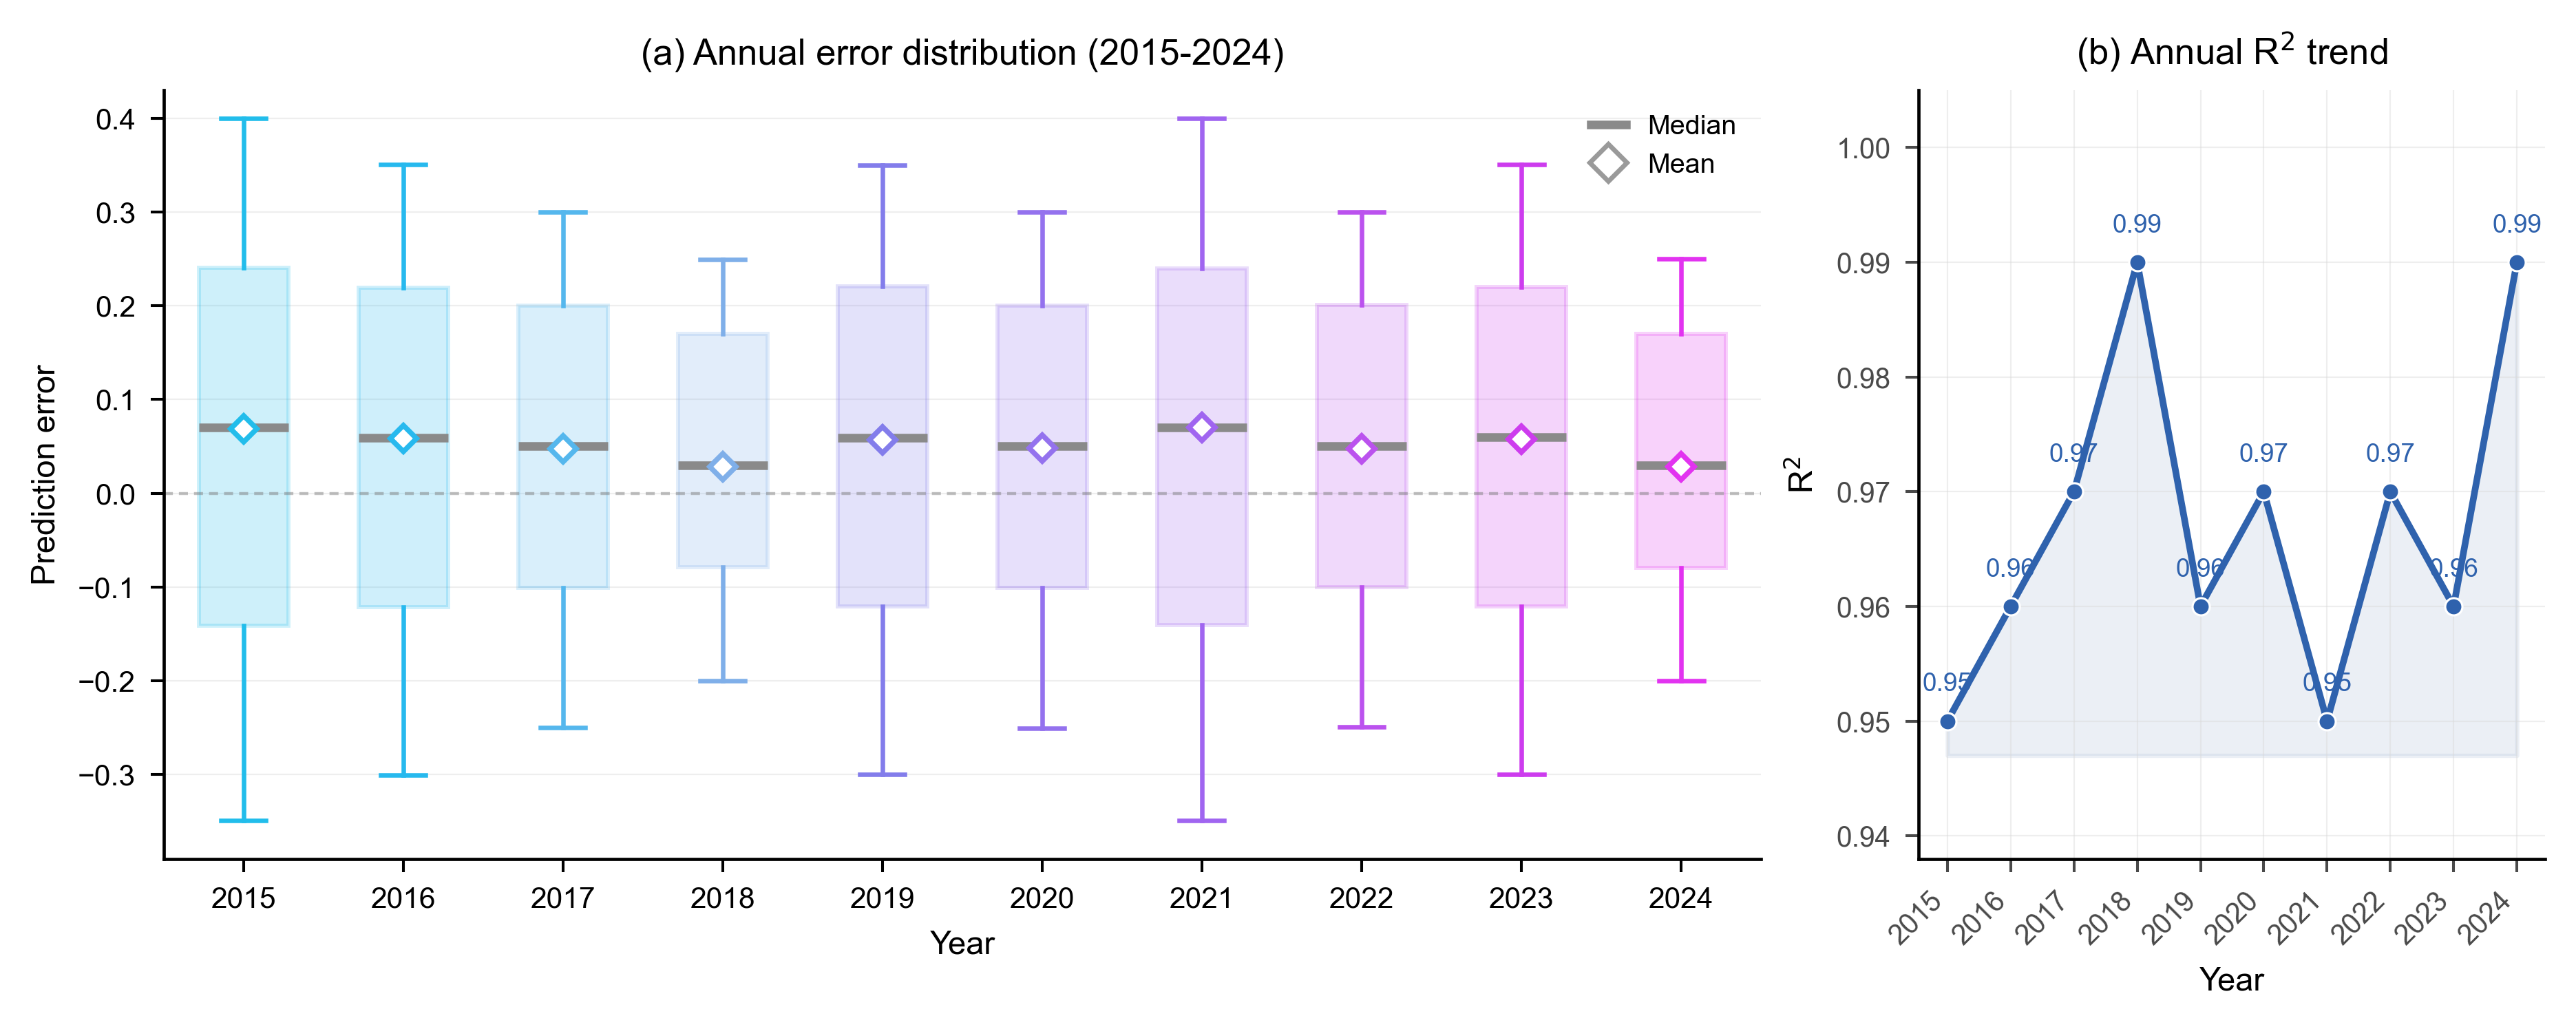
\includegraphics[width=0.98\linewidth]{../../results/figures/supporting/result2_annual_error_distribution_r2.png}
\caption{Annual prediction-error distribution and annual $R^2$ trend for the 2015--2024 preview. Panel (a) summarizes annual error distributions by whisker, quartile, median and mean values; panel (b) reports the annual $R^2$ sequence.}
\label{fig:annual-error-distribution-r2-trend}
\end{figure}

\begin{table}[htbp]
\centering
\caption{Source table data corresponding to the annual evaluation metrics, prediction-error distribution and annual $R^2$ trend.}
\label{tab:annual-error-distribution-r2-stats}
\scriptsize
\setlength{\tabcolsep}{2.4pt}
\renewcommand{\arraystretch}{1.08}
\resizebox{\textwidth}{!}{%
\begin{tabular}{rrrrrrrrrr}
\toprule
Year & MAE & RMSE & $R^2$ & Lower whisker & Q1 & Median & Mean marker & Q3 & Upper whisker \\
\midrule
2015 & 0.0685 & 0.1268 & 0.9766 & -0.3494 & -0.1412 & 0.0669 & 0.0685 & 0.2408 & 0.4003 \\
2016 & 0.0582 & 0.1174 & 0.9812 & -0.3006 & -0.1214 & 0.0567 & 0.0582 & 0.2196 & 0.3507 \\
2017 & 0.0476 & 0.1096 & 0.9854 & -0.2502 & -0.1007 & 0.0491 & 0.0476 & 0.2005 & 0.3001 \\
2018 & 0.0284 & 0.1012 & 0.9916 & -0.2004 & -0.0792 & 0.0312 & 0.0284 & 0.1698 & 0.2495 \\
2019 & 0.0567 & 0.1161 & 0.9827 & -0.2997 & -0.1205 & 0.0554 & 0.0567 & 0.2209 & 0.3502 \\
2020 & 0.0478 & 0.1089 & 0.9861 & -0.2508 & -0.1011 & 0.0484 & 0.0478 & 0.2002 & 0.3004 \\
2021 & 0.0699 & 0.1285 & 0.9758 & -0.3491 & -0.1406 & 0.0711 & 0.0699 & 0.2397 & 0.3998 \\
2022 & 0.0475 & 0.1082 & 0.9868 & -0.2496 & -0.1003 & 0.0492 & 0.0475 & 0.2007 & 0.3000 \\
2023 & 0.0576 & 0.1158 & 0.9824 & -0.3003 & -0.1208 & 0.0568 & 0.0576 & 0.2201 & 0.3505 \\
2024 & 0.0285 & 0.0864 & 0.9921 & -0.1998 & -0.0797 & 0.0293 & 0.0285 & 0.1703 & 0.2502 \\
\bottomrule
\end{tabular}%
}
\end{table}

\noindent
Across the 2015--2024 sequence, the mean annual MAE is 0.05107$^\circ$C, the mean annual RMSE is 0.11189$^\circ$C and the mean annual $R^2$ is 0.98407.
The annual $R^2$ values range from 0.9758 to 0.9921, with the highest values appearing in 2018 and 2024.

\clearpage
\section{Depth-Resolved Reconstruction Accuracy}
\label{sec:depth-resolved-reconstruction-accuracy}

\noindent
This section records the 1~m depth-resolved accuracy profile used to support the vertical reconstruction-error assessment.
The complete source table is retained as \texttt{data/supporting/result2\_depth\_accuracy\_1m.csv}; it contains 3867 depth levels from 159 to 4025~m and 27,107,729 depth-bin samples.
The columns in the source table are depth, sample count, MAE, RMSE and the corresponding depth-bin $R^2$.

\begin{figure}[htbp]
\centering
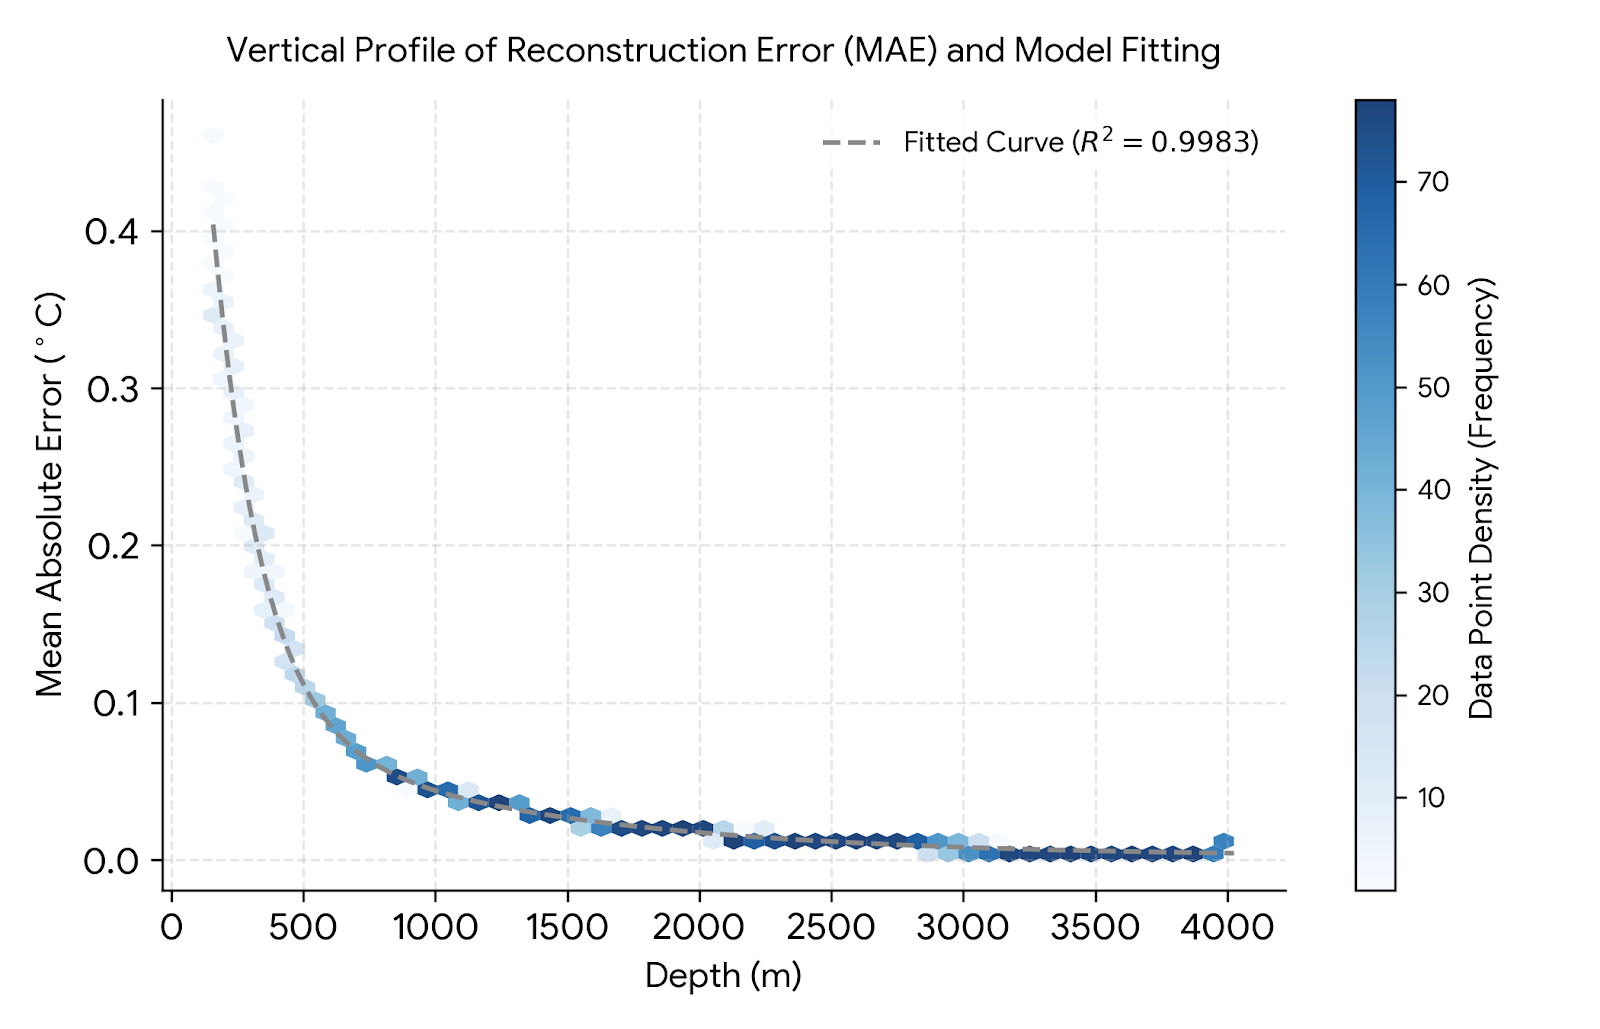
\includegraphics[width=0.92\linewidth]{../../results/figures/supporting/result2_vertical_profile_reconstruction_error.png}
\caption{Vertical profile of reconstruction error and fitted depth-decay curve. The horizontal coordinate is depth, the vertical coordinate is MAE, and the point color represents the depth-bin data density. The dashed curve reports the fitted vertical error profile with $R^2=0.9983$.}
\label{fig:depth-resolved-reconstruction-error}
\end{figure}

\noindent
Figure~\ref{fig:depth-resolved-reconstruction-error} shows a rapid reduction in reconstruction error from the upper-ocean depth range toward the deeper profile.
Across the complete 1~m source record, the count-weighted MAE is 0.051075$^\circ$C and the count-weighted RMSE is 0.065764$^\circ$C.
The largest depth-bin MAE occurs near 166~m, while the lowest MAE occurs near 3833~m.

\begin{table}[htbp]
\centering
\caption{Depth-band summary of the 1~m vertical reconstruction-accuracy source records. MAE and RMSE are count-weighted within each depth band.}
\label{tab:depth-accuracy-band-summary}
\small
\setlength{\tabcolsep}{4.5pt}
\renewcommand{\arraystretch}{1.08}
\begin{tabular}{rrrrr}
\toprule
Depth band (m) & Number of 1~m bins & Sample count & MAE & RMSE \\
\midrule
150--250 & 91 & 697476 & 0.3279 & 0.4463 \\
250--500 & 250 & 2434715 & 0.1743 & 0.2339 \\
500--750 & 250 & 2543831 & 0.0829 & 0.1040 \\
750--1000 & 250 & 2672883 & 0.0518 & 0.0639 \\
1000--1500 & 500 & 5415302 & 0.0348 & 0.0430 \\
1500--2000 & 500 & 5416099 & 0.0221 & 0.0269 \\
2000--2500 & 500 & 2243349 & 0.0148 & 0.0177 \\
2500--3000 & 500 & 2090406 & 0.0094 & 0.0114 \\
3000--3500 & 500 & 1880966 & 0.0063 & 0.0075 \\
3500--4025 & 526 & 1712702 & 0.0052 & 0.0062 \\
\bottomrule
\end{tabular}
\end{table}

\clearpage
\begin{table}[htbp]
\centering
\caption{Representative 1~m depth-bin records sampled from the complete vertical reconstruction-accuracy source table.}
\label{tab:depth-accuracy-representative-records}
\small
\setlength{\tabcolsep}{5pt}
\renewcommand{\arraystretch}{1.08}
\begin{tabular}{rrrrr}
\toprule
Depth (m) & Sample count & MAE & RMSE & Depth-bin $R^2$ \\
\midrule
160 & 564 & 0.4569 & 0.5564 & -0.0003 \\
200 & 7895 & 0.3358 & 0.4593 & -0.0021 \\
250 & 8928 & 0.2722 & 0.3804 & -0.0002 \\
300 & 9289 & 0.2203 & 0.3070 & -0.0012 \\
400 & 9966 & 0.1526 & 0.1997 & -0.0009 \\
500 & 10042 & 0.1103 & 0.1405 & -0.0012 \\
750 & 10523 & 0.0619 & 0.0764 & -0.0000 \\
1000 & 10791 & 0.0444 & 0.0549 & -0.0245 \\
1500 & 10761 & 0.0252 & 0.0315 & -0.0516 \\
2000 & 10890 & 0.0186 & 0.0223 & -0.0565 \\
2500 & 4406 & 0.0115 & 0.0140 & -0.0050 \\
3000 & 3972 & 0.0077 & 0.0093 & -0.0033 \\
3500 & 3452 & 0.0055 & 0.0064 & -0.4156 \\
4000 & 1000 & 0.0102 & 0.0105 & -18.3876 \\
\bottomrule
\end{tabular}
\end{table}

\noindent
The representative records and band summaries show the same depth-dependent error attenuation as the fitted curve in Figure~\ref{fig:depth-resolved-reconstruction-error}.
The depth-bin $R^2$ column is retained from the source table for traceability; in very deep low-variance bins it is more sensitive to local variance than MAE and RMSE, so the vertical profile interpretation is primarily based on MAE, RMSE and the fitted MAE-depth relation.

\clearpage
% Auto-generated compact landscape table from supporting_data/result2_depth_accuracy_1m.csv.
% Four depth records are placed on each table row to reduce PDF page count.
\begin{landscape}
\subsection{Complete 1~m Depth-Resolved Source Table}
\label{subsec:complete-depth-accuracy-source-table}

\noindent
Table~\ref{tab:depth-accuracy-full-1m-compact} compiles the complete 1~m source record into the PDF using a compact four-block landscape layout.
Each table row contains up to four independent depth-bin records, which reduces page count while preserving direct lookup by depth.

\vspace{0.5em}
\begingroup
\tiny
\setlength{\tabcolsep}{2.2pt}
\renewcommand{\arraystretch}{0.86}
\begin{longtable}{rrrrrrrrrrrrrrrrrrrr}
\caption{Complete 1~m depth-resolved reconstruction-accuracy source table in compact four-block layout. Each row contains up to four independent depth-bin records from \texttt{supporting\_data/result2\_depth\_accuracy\_1m.csv}.}\label{tab:depth-accuracy-full-1m-compact}\\
\toprule
Depth & $n$ & MAE & RMSE & $R^2$ & Depth & $n$ & MAE & RMSE & $R^2$ & Depth & $n$ & MAE & RMSE & $R^2$ & Depth & $n$ & MAE & RMSE & $R^2$ \\
\cmidrule(lr){1-5} \cmidrule(lr){6-10} \cmidrule(lr){11-15} \cmidrule(lr){16-20}
\endfirsthead
\caption[]{Complete 1~m depth-resolved reconstruction-accuracy source table continued.}\\
\toprule
Depth & $n$ & MAE & RMSE & $R^2$ & Depth & $n$ & MAE & RMSE & $R^2$ & Depth & $n$ & MAE & RMSE & $R^2$ & Depth & $n$ & MAE & RMSE & $R^2$ \\
\cmidrule(lr){1-5} \cmidrule(lr){6-10} \cmidrule(lr){11-15} \cmidrule(lr){16-20}
\endhead
\midrule
\multicolumn{20}{r}{Continued on next landscape page}\\
\endfoot
\bottomrule
\endlastfoot
159 & 117 & 0.37157 & 0.42636 & -0.7273 & 160 & 564 & 0.45688 & 0.55635 & -0.0003 & 161 & 2757 & 0.41363 & 0.52234 & -0.0176 & 162 & 4755 & 0.37918 & 0.49003 & -0.0332 \\
163 & 5112 & 0.37805 & 0.48918 & -0.0231 & 164 & 4143 & 0.35149 & 0.45679 & -0.0044 & 165 & 4284 & 0.42910 & 0.54724 & -0.0082 & 166 & 5751 & 0.46069 & 0.57831 & -0.0487 \\
167 & 7228 & 0.41707 & 0.53378 & -0.0376 & 168 & 7424 & 0.39479 & 0.50629 & -0.0200 & 169 & 6749 & 0.40058 & 0.51100 & -0.0233 & 170 & 6473 & 0.38900 & 0.50230 & -0.0127 \\
171 & 7037 & 0.36708 & 0.48421 & -0.0115 & 172 & 7692 & 0.34965 & 0.46851 & -0.0099 & 173 & 7588 & 0.35097 & 0.47115 & -0.0056 & 174 & 7175 & 0.35974 & 0.47781 & -0.0049 \\
175 & 7198 & 0.36170 & 0.48269 & -0.0040 & 176 & 7213 & 0.36125 & 0.48050 & -0.0031 & 177 & 7187 & 0.36193 & 0.48175 & -0.0015 & 178 & 7238 & 0.36124 & 0.48134 & -0.0012 \\
179 & 7305 & 0.35849 & 0.48044 & -0.0006 & 180 & 7252 & 0.35498 & 0.47528 & -0.0007 & 181 & 7323 & 0.35773 & 0.47879 & -0.0001 & 182 & 7371 & 0.35511 & 0.47669 & -0.0002 \\
183 & 7373 & 0.35070 & 0.47179 & -0.0002 & 184 & 7448 & 0.34819 & 0.47000 & -0.0000 & 185 & 7413 & 0.35020 & 0.47185 & -0.0000 & 186 & 7483 & 0.34739 & 0.46933 & -0.0002 \\
187 & 7572 & 0.34433 & 0.46680 & -0.0001 & 188 & 7696 & 0.34677 & 0.47013 & -0.0002 & 189 & 7681 & 0.34327 & 0.46762 & -0.0006 & 190 & 7738 & 0.34575 & 0.47075 & -0.0012 \\
191 & 7681 & 0.34557 & 0.46928 & -0.0020 & 192 & 7708 & 0.34753 & 0.47153 & -0.0013 & 193 & 7632 & 0.34645 & 0.47092 & -0.0020 & 194 & 7745 & 0.34499 & 0.46867 & -0.0021 \\
195 & 7697 & 0.34259 & 0.46643 & -0.0019 & 196 & 7734 & 0.34323 & 0.46543 & -0.0017 & 197 & 7761 & 0.34209 & 0.46553 & -0.0011 & 198 & 7825 & 0.33913 & 0.46238 & -0.0018 \\
199 & 7930 & 0.33750 & 0.46018 & -0.0019 & 200 & 7895 & 0.33583 & 0.45926 & -0.0021 & 201 & 7981 & 0.33811 & 0.46002 & -0.0021 & 202 & 8041 & 0.33384 & 0.45656 & -0.0025 \\
203 & 8129 & 0.33057 & 0.45285 & -0.0025 & 204 & 8155 & 0.33005 & 0.45301 & -0.0031 & 205 & 8162 & 0.33104 & 0.45476 & -0.0029 & 206 & 8241 & 0.32934 & 0.45462 & -0.0041 \\
207 & 8055 & 0.33232 & 0.45691 & -0.0046 & 208 & 8133 & 0.33156 & 0.45513 & -0.0041 & 209 & 8090 & 0.32816 & 0.45045 & -0.0035 & 210 & 8203 & 0.32555 & 0.44846 & -0.0044 \\
211 & 8154 & 0.32565 & 0.44785 & -0.0032 & 212 & 8137 & 0.32382 & 0.44617 & -0.0033 & 213 & 8296 & 0.32297 & 0.44427 & -0.0038 & 214 & 8232 & 0.32109 & 0.44201 & -0.0030 \\
215 & 8338 & 0.31991 & 0.44027 & -0.0027 & 216 & 8294 & 0.31909 & 0.43936 & -0.0028 & 217 & 8371 & 0.31572 & 0.43564 & -0.0042 & 218 & 8416 & 0.31195 & 0.43201 & -0.0031 \\
219 & 8467 & 0.31354 & 0.43256 & -0.0033 & 220 & 8537 & 0.31273 & 0.43185 & -0.0033 & 221 & 8553 & 0.31043 & 0.43037 & -0.0031 & 222 & 8498 & 0.31209 & 0.43365 & -0.0049 \\
223 & 8401 & 0.31155 & 0.43091 & -0.0035 & 224 & 8504 & 0.31318 & 0.43232 & -0.0032 & 225 & 8500 & 0.30872 & 0.42665 & -0.0023 & 226 & 8508 & 0.30841 & 0.42657 & -0.0027 \\
227 & 8515 & 0.30539 & 0.42286 & -0.0023 & 228 & 8461 & 0.30466 & 0.42228 & -0.0023 & 229 & 8540 & 0.30488 & 0.42208 & -0.0031 & 230 & 8688 & 0.30090 & 0.41544 & -0.0022 \\
231 & 8676 & 0.29837 & 0.41369 & -0.0016 & 232 & 8602 & 0.29834 & 0.41400 & -0.0023 & 233 & 8724 & 0.29476 & 0.40913 & -0.0016 & 234 & 8676 & 0.29466 & 0.40895 & -0.0015 \\
235 & 8754 & 0.29280 & 0.40647 & -0.0018 & 236 & 8735 & 0.29312 & 0.40784 & -0.0018 & 237 & 8861 & 0.29261 & 0.40701 & -0.0022 & 238 & 8853 & 0.29044 & 0.40318 & -0.0015 \\
239 & 8842 & 0.29105 & 0.40530 & -0.0015 & 240 & 8759 & 0.28699 & 0.39929 & -0.0017 & 241 & 8854 & 0.28654 & 0.39951 & -0.0008 & 242 & 8736 & 0.28554 & 0.39812 & -0.0007 \\
243 & 8788 & 0.28287 & 0.39380 & -0.0006 & 244 & 8768 & 0.28058 & 0.39138 & -0.0006 & 245 & 8744 & 0.27878 & 0.38996 & -0.0008 & 246 & 8884 & 0.27637 & 0.38689 & -0.0006 \\
247 & 8896 & 0.27667 & 0.38488 & -0.0001 & 248 & 8897 & 0.27444 & 0.38329 & -0.0003 & 249 & 8879 & 0.27353 & 0.38275 & -0.0003 & 250 & 8928 & 0.27217 & 0.38038 & -0.0002 \\
251 & 8928 & 0.27329 & 0.38235 & -0.0002 & 252 & 9006 & 0.27150 & 0.37911 & -0.0001 & 253 & 9034 & 0.27100 & 0.37976 & -0.0006 & 254 & 9046 & 0.26944 & 0.37628 & -0.0001 \\
255 & 9016 & 0.26846 & 0.37584 & -0.0001 & 256 & 8988 & 0.26842 & 0.37586 & -0.0002 & 257 & 8960 & 0.26753 & 0.37378 & -0.0000 & 258 & 8922 & 0.26606 & 0.37340 & -0.0001 \\
259 & 9035 & 0.26333 & 0.36784 & -0.0000 & 260 & 8994 & 0.26165 & 0.36584 & -0.0000 & 261 & 8986 & 0.25977 & 0.36384 & -0.0000 & 262 & 9056 & 0.25785 & 0.36168 & -0.0000 \\
263 & 9001 & 0.25755 & 0.36133 & -0.0000 & 264 & 9066 & 0.25750 & 0.36104 & -0.0000 & 265 & 9106 & 0.25424 & 0.35672 & -0.0001 & 266 & 9077 & 0.25422 & 0.35682 & -0.0000 \\
267 & 9137 & 0.25538 & 0.35780 & -0.0000 & 268 & 9067 & 0.25033 & 0.35187 & -0.0000 & 269 & 9041 & 0.24957 & 0.35217 & -0.0000 & 270 & 9215 & 0.25050 & 0.35192 & -0.0000 \\
271 & 9193 & 0.24925 & 0.34930 & -0.0002 & 272 & 9134 & 0.24769 & 0.34833 & -0.0001 & 273 & 9079 & 0.24536 & 0.34493 & -0.0001 & 274 & 9115 & 0.24562 & 0.34552 & -0.0001 \\
275 & 9080 & 0.24469 & 0.34510 & -0.0001 & 276 & 9118 & 0.24278 & 0.34134 & -0.0002 & 277 & 9152 & 0.24116 & 0.34011 & -0.0000 & 278 & 9168 & 0.23913 & 0.33674 & -0.0002 \\
279 & 9207 & 0.23887 & 0.33560 & -0.0005 & 280 & 9232 & 0.23839 & 0.33512 & -0.0005 & 281 & 9222 & 0.23900 & 0.33506 & -0.0004 & 282 & 9316 & 0.23726 & 0.33240 & -0.0005 \\
283 & 9216 & 0.23612 & 0.33071 & -0.0002 & 284 & 9152 & 0.23526 & 0.32963 & -0.0006 & 285 & 9275 & 0.23625 & 0.33090 & -0.0003 & 286 & 9295 & 0.23346 & 0.32663 & -0.0005 \\
287 & 9213 & 0.23139 & 0.32411 & -0.0007 & 288 & 9300 & 0.23289 & 0.32569 & -0.0005 & 289 & 9293 & 0.22974 & 0.32195 & -0.0005 & 290 & 9204 & 0.23162 & 0.32375 & -0.0008 \\
291 & 9257 & 0.22852 & 0.31999 & -0.0007 & 292 & 9350 & 0.22764 & 0.31893 & -0.0007 & 293 & 9311 & 0.22645 & 0.31801 & -0.0007 & 294 & 9307 & 0.22591 & 0.31577 & -0.0010 \\
295 & 9331 & 0.22343 & 0.31276 & -0.0011 & 296 & 9365 & 0.22215 & 0.31108 & -0.0006 & 297 & 9395 & 0.22198 & 0.30966 & -0.0007 & 298 & 9299 & 0.22167 & 0.30882 & -0.0011 \\
299 & 9361 & 0.22252 & 0.30959 & -0.0008 & 300 & 9289 & 0.22034 & 0.30702 & -0.0012 & 301 & 9356 & 0.22026 & 0.30635 & -0.0009 & 302 & 9334 & 0.21803 & 0.30415 & -0.0006 \\
303 & 9383 & 0.21802 & 0.30347 & -0.0008 & 304 & 9437 & 0.21685 & 0.30102 & -0.0012 & 305 & 9342 & 0.21665 & 0.30063 & -0.0008 & 306 & 9341 & 0.21552 & 0.30041 & -0.0008 \\
307 & 9379 & 0.21654 & 0.30022 & -0.0010 & 308 & 9331 & 0.21430 & 0.29698 & -0.0008 & 309 & 9293 & 0.21426 & 0.29724 & -0.0006 & 310 & 9381 & 0.21200 & 0.29426 & -0.0008 \\
311 & 9481 & 0.21156 & 0.29295 & -0.0010 & 312 & 9411 & 0.20960 & 0.28976 & -0.0008 & 313 & 9410 & 0.20910 & 0.28902 & -0.0015 & 314 & 9432 & 0.20913 & 0.28816 & -0.0013 \\
315 & 9375 & 0.20984 & 0.28941 & -0.0008 & 316 & 9378 & 0.20808 & 0.28656 & -0.0011 & 317 & 9484 & 0.20684 & 0.28459 & -0.0015 & 318 & 9461 & 0.20572 & 0.28399 & -0.0011 \\
319 & 9403 & 0.20484 & 0.28268 & -0.0009 & 320 & 9458 & 0.20432 & 0.28142 & -0.0010 & 321 & 9437 & 0.20468 & 0.28178 & -0.0011 & 322 & 9456 & 0.20486 & 0.28050 & -0.0014 \\
323 & 9439 & 0.20383 & 0.27802 & -0.0022 & 324 & 9737 & 0.20735 & 0.28077 & -0.0042 & 325 & 10108 & 0.20999 & 0.28029 & -0.0111 & 326 & 10146 & 0.21085 & 0.28105 & -0.0147 \\
327 & 9970 & 0.20466 & 0.27484 & -0.0081 & 328 & 9832 & 0.20437 & 0.27633 & -0.0057 & 329 & 9809 & 0.20154 & 0.27157 & -0.0065 & 330 & 9868 & 0.20255 & 0.27199 & -0.0064 \\
331 & 9799 & 0.20102 & 0.27074 & -0.0060 & 332 & 9795 & 0.20041 & 0.27003 & -0.0050 & 333 & 9843 & 0.19947 & 0.26794 & -0.0059 & 334 & 9808 & 0.19791 & 0.26675 & -0.0053 \\
335 & 9749 & 0.19745 & 0.26602 & -0.0050 & 336 & 9842 & 0.19601 & 0.26379 & -0.0054 & 337 & 9868 & 0.19587 & 0.26331 & -0.0050 & 338 & 9824 & 0.19490 & 0.26209 & -0.0043 \\
339 & 9883 & 0.19384 & 0.26031 & -0.0051 & 340 & 9880 & 0.19310 & 0.25933 & -0.0043 & 341 & 9806 & 0.19267 & 0.25858 & -0.0044 & 342 & 9878 & 0.19197 & 0.25710 & -0.0054 \\
343 & 9870 & 0.18968 & 0.25532 & -0.0036 & 344 & 9832 & 0.18912 & 0.25422 & -0.0039 & 345 & 9834 & 0.18803 & 0.25246 & -0.0047 & 346 & 9841 & 0.18830 & 0.25285 & -0.0044 \\
347 & 9821 & 0.18780 & 0.25107 & -0.0039 & 348 & 9796 & 0.18597 & 0.24909 & -0.0031 & 349 & 9819 & 0.18499 & 0.24763 & -0.0039 & 350 & 10265 & 0.18382 & 0.24597 & -0.0013 \\
351 & 9908 & 0.18508 & 0.24733 & -0.0038 & 352 & 9891 & 0.18213 & 0.24379 & -0.0029 & 353 & 9886 & 0.18346 & 0.24515 & -0.0034 & 354 & 9908 & 0.18266 & 0.24368 & -0.0034 \\
355 & 9903 & 0.18089 & 0.24073 & -0.0035 & 356 & 9878 & 0.18032 & 0.24036 & -0.0031 & 357 & 9911 & 0.17829 & 0.23779 & -0.0027 & 358 & 9963 & 0.18003 & 0.24023 & -0.0024 \\
359 & 9889 & 0.17691 & 0.23564 & -0.0029 & 360 & 9902 & 0.17581 & 0.23439 & -0.0027 & 361 & 9888 & 0.17644 & 0.23473 & -0.0028 & 362 & 9947 & 0.17564 & 0.23388 & -0.0035 \\
363 & 9883 & 0.17423 & 0.23177 & -0.0033 & 364 & 9913 & 0.17340 & 0.23081 & -0.0030 & 365 & 9906 & 0.17297 & 0.22968 & -0.0029 & 366 & 9935 & 0.17270 & 0.22991 & -0.0026 \\
367 & 9907 & 0.17218 & 0.22876 & -0.0026 & 368 & 9973 & 0.17098 & 0.22705 & -0.0028 & 369 & 9991 & 0.17061 & 0.22636 & -0.0028 & 370 & 9967 & 0.17105 & 0.22687 & -0.0020 \\
371 & 9957 & 0.16887 & 0.22380 & -0.0019 & 372 & 9899 & 0.16904 & 0.22356 & -0.0029 & 373 & 9888 & 0.16781 & 0.22240 & -0.0021 & 374 & 9836 & 0.16741 & 0.22229 & -0.0014 \\
375 & 9958 & 0.16637 & 0.22096 & -0.0013 & 376 & 9895 & 0.16569 & 0.21902 & -0.0019 & 377 & 9916 & 0.16494 & 0.21812 & -0.0027 & 378 & 9877 & 0.16581 & 0.21981 & -0.0016 \\
379 & 9855 & 0.16435 & 0.21713 & -0.0018 & 380 & 9933 & 0.16375 & 0.21626 & -0.0023 & 381 & 9951 & 0.16205 & 0.21396 & -0.0027 & 382 & 9960 & 0.16275 & 0.21538 & -0.0016 \\
383 & 9942 & 0.16090 & 0.21290 & -0.0024 & 384 & 10010 & 0.16146 & 0.21304 & -0.0018 & 385 & 9891 & 0.16045 & 0.21183 & -0.0016 & 386 & 9944 & 0.16048 & 0.21224 & -0.0012 \\
387 & 9903 & 0.15903 & 0.20942 & -0.0018 & 388 & 9927 & 0.15843 & 0.20911 & -0.0017 & 389 & 9927 & 0.15711 & 0.20728 & -0.0017 & 390 & 9890 & 0.15712 & 0.20784 & -0.0007 \\
391 & 10026 & 0.15726 & 0.20738 & -0.0012 & 392 & 9878 & 0.15718 & 0.20656 & -0.0009 & 393 & 9922 & 0.15498 & 0.20389 & -0.0010 & 394 & 9870 & 0.15607 & 0.20548 & -0.0010 \\
395 & 9953 & 0.15538 & 0.20407 & -0.0011 & 396 & 9898 & 0.15525 & 0.20330 & -0.0010 & 397 & 9910 & 0.15423 & 0.20177 & -0.0015 & 398 & 10004 & 0.15342 & 0.20084 & -0.0008 \\
399 & 9950 & 0.15309 & 0.20036 & -0.0010 & 400 & 9966 & 0.15264 & 0.19972 & -0.0009 & 401 & 9922 & 0.15187 & 0.19846 & -0.0006 & 402 & 9917 & 0.15175 & 0.19861 & -0.0004 \\
403 & 9979 & 0.15078 & 0.19707 & -0.0006 & 404 & 9911 & 0.15153 & 0.19758 & -0.0004 & 405 & 9938 & 0.14990 & 0.19535 & -0.0007 & 406 & 9933 & 0.15011 & 0.19566 & -0.0002 \\
407 & 9958 & 0.14960 & 0.19523 & -0.0003 & 408 & 9921 & 0.14903 & 0.19393 & -0.0004 & 409 & 9925 & 0.14811 & 0.19298 & -0.0004 & 410 & 9919 & 0.14792 & 0.19279 & -0.0002 \\
411 & 9895 & 0.14772 & 0.19200 & -0.0004 & 412 & 9948 & 0.14778 & 0.19177 & -0.0006 & 413 & 9939 & 0.14638 & 0.18987 & -0.0007 & 414 & 9969 & 0.14646 & 0.18971 & -0.0004 \\
415 & 9990 & 0.14533 & 0.18873 & -0.0004 & 416 & 9869 & 0.14518 & 0.18815 & -0.0003 & 417 & 10018 & 0.14404 & 0.18692 & -0.0002 & 418 & 9949 & 0.14546 & 0.18822 & -0.0003 \\
419 & 9935 & 0.14376 & 0.18588 & -0.0002 & 420 & 10011 & 0.14257 & 0.18442 & -0.0001 & 421 & 10002 & 0.14206 & 0.18361 & -0.0001 & 422 & 9910 & 0.14226 & 0.18379 & -0.0000 \\
423 & 9941 & 0.14257 & 0.18410 & -0.0001 & 424 & 9916 & 0.14180 & 0.18274 & -0.0001 & 425 & 9963 & 0.14164 & 0.18283 & -0.0000 & 426 & 9899 & 0.14115 & 0.18203 & -0.0001 \\
427 & 9938 & 0.14113 & 0.18183 & -0.0000 & 428 & 10001 & 0.14002 & 0.18022 & -0.0000 & 429 & 9958 & 0.13981 & 0.18010 & -0.0001 & 430 & 9978 & 0.13929 & 0.17892 & -0.0002 \\
431 & 10009 & 0.13910 & 0.17916 & -0.0001 & 432 & 10082 & 0.13811 & 0.17744 & -0.0002 & 433 & 9948 & 0.13811 & 0.17742 & -0.0000 & 434 & 9971 & 0.13782 & 0.17703 & -0.0000 \\
435 & 9967 & 0.13689 & 0.17545 & -0.0000 & 436 & 10009 & 0.13621 & 0.17477 & -0.0000 & 437 & 9941 & 0.13571 & 0.17385 & -0.0000 & 438 & 9977 & 0.13469 & 0.17275 & -0.0000 \\
439 & 9968 & 0.13474 & 0.17296 & -0.0000 & 440 & 9919 & 0.13490 & 0.17252 & -0.0000 & 441 & 9979 & 0.13409 & 0.17173 & -0.0000 & 442 & 9942 & 0.13407 & 0.17177 & -0.0001 \\
443 & 10037 & 0.13455 & 0.17201 & -0.0000 & 444 & 9881 & 0.13259 & 0.16997 & -0.0000 & 445 & 10001 & 0.13226 & 0.16943 & -0.0000 & 446 & 10020 & 0.13243 & 0.16937 & -0.0000 \\
447 & 10022 & 0.13086 & 0.16771 & -0.0000 & 448 & 9988 & 0.13092 & 0.16762 & -0.0000 & 449 & 9992 & 0.13134 & 0.16823 & -0.0001 & 450 & 10018 & 0.13076 & 0.16698 & -0.0001 \\
451 & 10012 & 0.12943 & 0.16546 & -0.0000 & 452 & 9987 & 0.12908 & 0.16530 & -0.0000 & 453 & 9963 & 0.12923 & 0.16528 & -0.0001 & 454 & 10018 & 0.12796 & 0.16375 & -0.0000 \\
455 & 9951 & 0.12847 & 0.16397 & -0.0002 & 456 & 9954 & 0.12781 & 0.16339 & -0.0001 & 457 & 9980 & 0.12747 & 0.16303 & -0.0002 & 458 & 10064 & 0.12756 & 0.16333 & -0.0003 \\
459 & 9957 & 0.12722 & 0.16245 & -0.0001 & 460 & 9982 & 0.12635 & 0.16133 & -0.0002 & 461 & 9999 & 0.12621 & 0.16102 & -0.0001 & 462 & 10028 & 0.12576 & 0.16082 & -0.0002 \\
463 & 10047 & 0.12399 & 0.15912 & -0.0002 & 464 & 10017 & 0.12413 & 0.15823 & -0.0004 & 465 & 10028 & 0.12441 & 0.15895 & -0.0004 & 466 & 9997 & 0.12345 & 0.15779 & -0.0003 \\
467 & 10041 & 0.12261 & 0.15656 & -0.0003 & 468 & 9960 & 0.12266 & 0.15655 & -0.0003 & 469 & 9978 & 0.12230 & 0.15619 & -0.0003 & 470 & 10031 & 0.12174 & 0.15532 & -0.0006 \\
471 & 9975 & 0.12164 & 0.15515 & -0.0002 & 472 & 9996 & 0.12088 & 0.15454 & -0.0006 & 473 & 10003 & 0.12080 & 0.15415 & -0.0003 & 474 & 9993 & 0.12087 & 0.15426 & -0.0006 \\
475 & 9997 & 0.12066 & 0.15446 & -0.0013 & 476 & 10025 & 0.12012 & 0.15344 & -0.0005 & 477 & 10075 & 0.11918 & 0.15226 & -0.0008 & 478 & 10092 & 0.11837 & 0.15131 & -0.0006 \\
479 & 10046 & 0.11822 & 0.15117 & -0.0006 & 480 & 10012 & 0.11783 & 0.15013 & -0.0010 & 481 & 10104 & 0.11774 & 0.15023 & -0.0010 & 482 & 10061 & 0.11711 & 0.14944 & -0.0012 \\
483 & 10008 & 0.11638 & 0.14831 & -0.0006 & 484 & 9912 & 0.11640 & 0.14812 & -0.0008 & 485 & 10043 & 0.11594 & 0.14748 & -0.0007 & 486 & 10048 & 0.11541 & 0.14717 & -0.0009 \\
487 & 10056 & 0.11482 & 0.14611 & -0.0006 & 488 & 10025 & 0.11408 & 0.14541 & -0.0010 & 489 & 9965 & 0.11423 & 0.14555 & -0.0012 & 490 & 9988 & 0.11415 & 0.14561 & -0.0014 \\
491 & 10065 & 0.11371 & 0.14514 & -0.0020 & 492 & 10017 & 0.11294 & 0.14395 & -0.0011 & 493 & 10146 & 0.11254 & 0.14339 & -0.0013 & 494 & 10071 & 0.11205 & 0.14280 & -0.0013 \\
495 & 10074 & 0.11218 & 0.14334 & -0.0010 & 496 & 10110 & 0.11133 & 0.14204 & -0.0020 & 497 & 10088 & 0.11138 & 0.14196 & -0.0015 & 498 & 10019 & 0.11057 & 0.14106 & -0.0021 \\
499 & 10036 & 0.11036 & 0.14045 & -0.0014 & 500 & 10042 & 0.11033 & 0.14050 & -0.0012 & 501 & 10093 & 0.10938 & 0.13942 & -0.0012 & 502 & 10057 & 0.10978 & 0.13980 & -0.0013 \\
503 & 10050 & 0.10915 & 0.13897 & -0.0019 & 504 & 10011 & 0.10874 & 0.13842 & -0.0017 & 505 & 9938 & 0.10870 & 0.13840 & -0.0018 & 506 & 10040 & 0.10814 & 0.13790 & -0.0026 \\
507 & 9986 & 0.10828 & 0.13787 & -0.0022 & 508 & 10090 & 0.10814 & 0.13762 & -0.0019 & 509 & 10145 & 0.10716 & 0.13650 & -0.0024 & 510 & 10058 & 0.10671 & 0.13587 & -0.0020 \\
511 & 10044 & 0.10627 & 0.13557 & -0.0027 & 512 & 10092 & 0.10623 & 0.13531 & -0.0025 & 513 & 10134 & 0.10576 & 0.13468 & -0.0024 & 514 & 10058 & 0.10531 & 0.13424 & -0.0025 \\
515 & 10068 & 0.10516 & 0.13369 & -0.0020 & 516 & 9987 & 0.10444 & 0.13301 & -0.0025 & 517 & 10042 & 0.10479 & 0.13331 & -0.0026 & 518 & 10085 & 0.10415 & 0.13249 & -0.0025 \\
519 & 10077 & 0.10330 & 0.13137 & -0.0027 & 520 & 10025 & 0.10358 & 0.13162 & -0.0030 & 521 & 10001 & 0.10320 & 0.13129 & -0.0030 & 522 & 9980 & 0.10233 & 0.13030 & -0.0031 \\
523 & 10038 & 0.10293 & 0.13110 & -0.0032 & 524 & 10077 & 0.10229 & 0.13000 & -0.0026 & 525 & 10053 & 0.10170 & 0.12932 & -0.0032 & 526 & 10126 & 0.10170 & 0.12953 & -0.0041 \\
527 & 10094 & 0.10135 & 0.12898 & -0.0032 & 528 & 10071 & 0.10096 & 0.12828 & -0.0036 & 529 & 10123 & 0.10100 & 0.12851 & -0.0038 & 530 & 10030 & 0.10114 & 0.12857 & -0.0037 \\
531 & 10059 & 0.10057 & 0.12759 & -0.0031 & 532 & 10009 & 0.10048 & 0.12756 & -0.0042 & 533 & 10075 & 0.09973 & 0.12666 & -0.0031 & 534 & 10037 & 0.09933 & 0.12645 & -0.0038 \\
535 & 10058 & 0.09936 & 0.12589 & -0.0037 & 536 & 10011 & 0.09928 & 0.12579 & -0.0042 & 537 & 10026 & 0.09843 & 0.12494 & -0.0044 & 538 & 10006 & 0.09863 & 0.12505 & -0.0042 \\
539 & 10003 & 0.09879 & 0.12527 & -0.0043 & 540 & 10095 & 0.09809 & 0.12463 & -0.0045 & 541 & 10084 & 0.09818 & 0.12449 & -0.0048 & 542 & 10137 & 0.09784 & 0.12417 & -0.0047 \\
543 & 10140 & 0.09776 & 0.12403 & -0.0057 & 544 & 10075 & 0.09727 & 0.12327 & -0.0047 & 545 & 10079 & 0.09724 & 0.12324 & -0.0051 & 546 & 10069 & 0.09712 & 0.12285 & -0.0045 \\
547 & 9994 & 0.09669 & 0.12245 & -0.0044 & 548 & 10098 & 0.09622 & 0.12184 & -0.0049 & 549 & 10059 & 0.09630 & 0.12194 & -0.0056 & 550 & 10043 & 0.09587 & 0.12148 & -0.0049 \\
551 & 10013 & 0.09589 & 0.12132 & -0.0062 & 552 & 10035 & 0.09521 & 0.12052 & -0.0061 & 553 & 10003 & 0.09548 & 0.12059 & -0.0055 & 554 & 10065 & 0.09528 & 0.12047 & -0.0056 \\
555 & 10063 & 0.09430 & 0.11936 & -0.0052 & 556 & 10069 & 0.09480 & 0.11999 & -0.0070 & 557 & 10063 & 0.09435 & 0.11913 & -0.0059 & 558 & 10162 & 0.09451 & 0.11941 & -0.0069 \\
559 & 10127 & 0.09420 & 0.11904 & -0.0063 & 560 & 10077 & 0.09422 & 0.11879 & -0.0067 & 561 & 10060 & 0.09372 & 0.11850 & -0.0068 & 562 & 10029 & 0.09370 & 0.11837 & -0.0066 \\
563 & 10040 & 0.09365 & 0.11808 & -0.0071 & 564 & 10037 & 0.09322 & 0.11762 & -0.0062 & 565 & 10097 & 0.09282 & 0.11704 & -0.0070 & 566 & 10010 & 0.09250 & 0.11671 & -0.0073 \\
567 & 10024 & 0.09234 & 0.11626 & -0.0066 & 568 & 10002 & 0.09219 & 0.11613 & -0.0072 & 569 & 10087 & 0.09187 & 0.11548 & -0.0060 & 570 & 10042 & 0.09171 & 0.11549 & -0.0074 \\
571 & 10052 & 0.09201 & 0.11583 & -0.0078 & 572 & 10069 & 0.09110 & 0.11459 & -0.0071 & 573 & 10066 & 0.09150 & 0.11500 & -0.0081 & 574 & 10145 & 0.09122 & 0.11473 & -0.0087 \\
575 & 10074 & 0.09093 & 0.11448 & -0.0081 & 576 & 10040 & 0.09075 & 0.11424 & -0.0083 & 577 & 10106 & 0.09072 & 0.11424 & -0.0089 & 578 & 10060 & 0.09034 & 0.11345 & -0.0084 \\
579 & 10059 & 0.09021 & 0.11349 & -0.0088 & 580 & 10085 & 0.08978 & 0.11290 & -0.0089 & 581 & 10082 & 0.08971 & 0.11291 & -0.0090 & 582 & 10101 & 0.08981 & 0.11286 & -0.0085 \\
583 & 10016 & 0.08924 & 0.11196 & -0.0079 & 584 & 10050 & 0.08937 & 0.11203 & -0.0088 & 585 & 10019 & 0.08895 & 0.11165 & -0.0105 & 586 & 10065 & 0.08888 & 0.11149 & -0.0086 \\
587 & 10042 & 0.08890 & 0.11158 & -0.0099 & 588 & 10066 & 0.08839 & 0.11110 & -0.0110 & 589 & 10124 & 0.08793 & 0.11032 & -0.0097 & 590 & 10169 & 0.08897 & 0.11167 & -0.0109 \\
591 & 10105 & 0.08837 & 0.11072 & -0.0103 & 592 & 10117 & 0.08810 & 0.11035 & -0.0102 & 593 & 10094 & 0.08789 & 0.11027 & -0.0101 & 594 & 10083 & 0.08774 & 0.10999 & -0.0102 \\
595 & 10089 & 0.08761 & 0.10998 & -0.0106 & 596 & 10114 & 0.08738 & 0.10968 & -0.0116 & 597 & 10085 & 0.08716 & 0.10927 & -0.0115 & 598 & 10065 & 0.08675 & 0.10859 & -0.0101 \\
599 & 10049 & 0.08694 & 0.10878 & -0.0125 & 600 & 10068 & 0.08609 & 0.10786 & -0.0100 & 601 & 10012 & 0.08635 & 0.10811 & -0.0120 & 602 & 10083 & 0.08634 & 0.10805 & -0.0128 \\
603 & 10057 & 0.08570 & 0.10746 & -0.0127 & 604 & 10134 & 0.08623 & 0.10776 & -0.0129 & 605 & 10104 & 0.08556 & 0.10695 & -0.0107 & 606 & 10083 & 0.08617 & 0.10804 & -0.0148 \\
607 & 10155 & 0.08526 & 0.10674 & -0.0113 & 608 & 10074 & 0.08532 & 0.10682 & -0.0125 & 609 & 10074 & 0.08509 & 0.10629 & -0.0121 & 610 & 10098 & 0.08508 & 0.10661 & -0.0136 \\
611 & 10155 & 0.08488 & 0.10584 & -0.0127 & 612 & 10114 & 0.08503 & 0.10624 & -0.0141 & 613 & 10008 & 0.08429 & 0.10526 & -0.0137 & 614 & 10048 & 0.08437 & 0.10540 & -0.0137 \\
615 & 10009 & 0.08388 & 0.10467 & -0.0138 & 616 & 10108 & 0.08375 & 0.10462 & -0.0130 & 617 & 10126 & 0.08322 & 0.10399 & -0.0138 & 618 & 10058 & 0.08315 & 0.10383 & -0.0142 \\
619 & 10143 & 0.08319 & 0.10397 & -0.0145 & 620 & 10078 & 0.08309 & 0.10399 & -0.0135 & 621 & 10156 & 0.08282 & 0.10352 & -0.0135 & 622 & 10130 & 0.08270 & 0.10355 & -0.0153 \\
623 & 10134 & 0.08262 & 0.10361 & -0.0140 & 624 & 10078 & 0.08242 & 0.10317 & -0.0150 & 625 & 10036 & 0.08220 & 0.10275 & -0.0141 & 626 & 10123 & 0.08202 & 0.10249 & -0.0133 \\
627 & 10088 & 0.08221 & 0.10241 & -0.0141 & 628 & 10106 & 0.08153 & 0.10197 & -0.0141 & 629 & 10011 & 0.08161 & 0.10189 & -0.0145 & 630 & 10105 & 0.08110 & 0.10119 & -0.0138 \\
631 & 10093 & 0.08137 & 0.10163 & -0.0131 & 632 & 10060 & 0.08149 & 0.10155 & -0.0148 & 633 & 10105 & 0.08069 & 0.10064 & -0.0124 & 634 & 10064 & 0.08082 & 0.10082 & -0.0143 \\
635 & 10059 & 0.08075 & 0.10089 & -0.0158 & 636 & 10148 & 0.08026 & 0.10026 & -0.0132 & 637 & 10123 & 0.08037 & 0.10025 & -0.0148 & 638 & 10080 & 0.08014 & 0.10014 & -0.0135 \\
639 & 10178 & 0.08012 & 0.09988 & -0.0127 & 640 & 10100 & 0.08005 & 0.10016 & -0.0153 & 641 & 10077 & 0.07979 & 0.09959 & -0.0141 & 642 & 10069 & 0.07936 & 0.09905 & -0.0133 \\
643 & 10108 & 0.07934 & 0.09902 & -0.0136 & 644 & 10051 & 0.07893 & 0.09841 & -0.0135 & 645 & 10128 & 0.07933 & 0.09916 & -0.0147 & 646 & 10104 & 0.07869 & 0.09820 & -0.0140 \\
647 & 10053 & 0.07860 & 0.09807 & -0.0125 & 648 & 10188 & 0.07833 & 0.09757 & -0.0140 & 649 & 10128 & 0.07789 & 0.09714 & -0.0130 & 650 & 10120 & 0.07810 & 0.09732 & -0.0118 \\
651 & 10109 & 0.07770 & 0.09696 & -0.0136 & 652 & 10162 & 0.07753 & 0.09670 & -0.0127 & 653 & 10050 & 0.07736 & 0.09634 & -0.0123 & 654 & 10144 & 0.07747 & 0.09668 & -0.0125 \\
655 & 10132 & 0.07677 & 0.09554 & -0.0127 & 656 & 10074 & 0.07723 & 0.09630 & -0.0137 & 657 & 10135 & 0.07693 & 0.09582 & -0.0121 & 658 & 10075 & 0.07660 & 0.09546 & -0.0130 \\
659 & 10094 & 0.07628 & 0.09504 & -0.0125 & 660 & 10164 & 0.07644 & 0.09530 & -0.0127 & 661 & 10114 & 0.07635 & 0.09529 & -0.0141 & 662 & 10136 & 0.07589 & 0.09433 & -0.0121 \\
663 & 10189 & 0.07532 & 0.09379 & -0.0123 & 664 & 10197 & 0.07554 & 0.09401 & -0.0105 & 665 & 10129 & 0.07517 & 0.09363 & -0.0123 & 666 & 10131 & 0.07477 & 0.09312 & -0.0105 \\
667 & 10153 & 0.07466 & 0.09298 & -0.0117 & 668 & 10168 & 0.07475 & 0.09284 & -0.0107 & 669 & 10192 & 0.07433 & 0.09239 & -0.0095 & 670 & 10155 & 0.07461 & 0.09275 & -0.0108 \\
671 & 10147 & 0.07412 & 0.09208 & -0.0091 & 672 & 10178 & 0.07451 & 0.09275 & -0.0105 & 673 & 10149 & 0.07364 & 0.09169 & -0.0100 & 674 & 10226 & 0.07379 & 0.09179 & -0.0103 \\
675 & 10162 & 0.07356 & 0.09148 & -0.0097 & 676 & 10224 & 0.07323 & 0.09088 & -0.0090 & 677 & 10241 & 0.07375 & 0.09157 & -0.0100 & 678 & 10244 & 0.07321 & 0.09088 & -0.0089 \\
679 & 10269 & 0.07281 & 0.09048 & -0.0083 & 680 & 10251 & 0.07263 & 0.09022 & -0.0090 & 681 & 10169 & 0.07265 & 0.09042 & -0.0088 & 682 & 10255 & 0.07232 & 0.08978 & -0.0071 \\
683 & 10209 & 0.07218 & 0.08956 & -0.0082 & 684 & 10303 & 0.07194 & 0.08924 & -0.0069 & 685 & 10303 & 0.07200 & 0.08935 & -0.0075 & 686 & 10241 & 0.07190 & 0.08919 & -0.0064 \\
687 & 10268 & 0.07155 & 0.08890 & -0.0081 & 688 & 10309 & 0.07157 & 0.08904 & -0.0070 & 689 & 10329 & 0.07117 & 0.08844 & -0.0074 & 690 & 10378 & 0.07119 & 0.08840 & -0.0068 \\
691 & 10322 & 0.07096 & 0.08793 & -0.0063 & 692 & 10294 & 0.07052 & 0.08756 & -0.0060 & 693 & 10374 & 0.07093 & 0.08806 & -0.0069 & 694 & 10411 & 0.07028 & 0.08717 & -0.0050 \\
695 & 10447 & 0.06994 & 0.08686 & -0.0053 & 696 & 10400 & 0.06950 & 0.08652 & -0.0059 & 697 & 10339 & 0.06966 & 0.08646 & -0.0062 & 698 & 10439 & 0.06968 & 0.08657 & -0.0055 \\
699 & 10317 & 0.06932 & 0.08604 & -0.0052 & 700 & 10430 & 0.06927 & 0.08598 & -0.0047 & 701 & 10309 & 0.06919 & 0.08575 & -0.0050 & 702 & 10409 & 0.06905 & 0.08564 & -0.0043 \\
703 & 10420 & 0.06868 & 0.08536 & -0.0046 & 704 & 10415 & 0.06871 & 0.08531 & -0.0040 & 705 & 10407 & 0.06852 & 0.08495 & -0.0034 & 706 & 10387 & 0.06813 & 0.08458 & -0.0033 \\
707 & 10455 & 0.06816 & 0.08455 & -0.0042 & 708 & 10417 & 0.06774 & 0.08406 & -0.0033 & 709 & 10391 & 0.06821 & 0.08453 & -0.0029 & 710 & 10445 & 0.06770 & 0.08402 & -0.0033 \\
711 & 10402 & 0.06753 & 0.08365 & -0.0031 & 712 & 10431 & 0.06729 & 0.08344 & -0.0026 & 713 & 10388 & 0.06694 & 0.08310 & -0.0030 & 714 & 10394 & 0.06742 & 0.08347 & -0.0026 \\
715 & 10505 & 0.06673 & 0.08263 & -0.0018 & 716 & 10349 & 0.06668 & 0.08268 & -0.0024 & 717 & 10376 & 0.06666 & 0.08252 & -0.0021 & 718 & 10468 & 0.06636 & 0.08217 & -0.0013 \\
719 & 10466 & 0.06651 & 0.08238 & -0.0017 & 720 & 10486 & 0.06610 & 0.08201 & -0.0019 & 721 & 10446 & 0.06595 & 0.08181 & -0.0015 & 722 & 10392 & 0.06561 & 0.08143 & -0.0017 \\
723 & 10419 & 0.06598 & 0.08169 & -0.0012 & 724 & 10401 & 0.06575 & 0.08132 & -0.0013 & 725 & 10501 & 0.06549 & 0.08113 & -0.0012 & 726 & 10483 & 0.06536 & 0.08090 & -0.0014 \\
727 & 10492 & 0.06516 & 0.08075 & -0.0014 & 728 & 10425 & 0.06486 & 0.08026 & -0.0009 & 729 & 10465 & 0.06498 & 0.08041 & -0.0009 & 730 & 10420 & 0.06463 & 0.07994 & -0.0009 \\
731 & 10510 & 0.06422 & 0.07954 & -0.0009 & 732 & 10372 & 0.06473 & 0.07988 & -0.0006 & 733 & 10441 & 0.06410 & 0.07923 & -0.0005 & 734 & 10439 & 0.06390 & 0.07898 & -0.0005 \\
735 & 10512 & 0.06412 & 0.07920 & -0.0005 & 736 & 10453 & 0.06379 & 0.07884 & -0.0004 & 737 & 10440 & 0.06394 & 0.07900 & -0.0006 & 738 & 10404 & 0.06343 & 0.07837 & -0.0002 \\
739 & 10500 & 0.06345 & 0.07831 & -0.0003 & 740 & 10540 & 0.06349 & 0.07829 & -0.0004 & 741 & 10455 & 0.06365 & 0.07847 & -0.0003 & 742 & 10426 & 0.06330 & 0.07815 & -0.0003 \\
743 & 10482 & 0.06296 & 0.07765 & -0.0002 & 744 & 10462 & 0.06262 & 0.07726 & -0.0001 & 745 & 10414 & 0.06249 & 0.07714 & -0.0002 & 746 & 10413 & 0.06274 & 0.07726 & -0.0001 \\
747 & 10483 & 0.06251 & 0.07706 & -0.0000 & 748 & 10436 & 0.06245 & 0.07699 & -0.0001 & 749 & 10494 & 0.06186 & 0.07636 & -0.0000 & 750 & 10523 & 0.06193 & 0.07638 & -0.0000 \\
751 & 10589 & 0.06159 & 0.07600 & -0.0000 & 752 & 10461 & 0.06174 & 0.07618 & -0.0000 & 753 & 10524 & 0.06155 & 0.07608 & -0.0000 & 754 & 10414 & 0.06135 & 0.07576 & -0.0000 \\
755 & 10495 & 0.06124 & 0.07562 & -0.0000 & 756 & 10497 & 0.06124 & 0.07548 & -0.0000 & 757 & 10453 & 0.06105 & 0.07539 & -0.0000 & 758 & 10468 & 0.06068 & 0.07496 & -0.0001 \\
759 & 10497 & 0.06109 & 0.07533 & -0.0000 & 760 & 10485 & 0.06106 & 0.07534 & -0.0001 & 761 & 10446 & 0.06066 & 0.07493 & -0.0002 & 762 & 10558 & 0.06036 & 0.07458 & -0.0002 \\
763 & 10519 & 0.06062 & 0.07479 & -0.0002 & 764 & 10491 & 0.06055 & 0.07474 & -0.0002 & 765 & 10478 & 0.05971 & 0.07379 & -0.0004 & 766 & 10502 & 0.05980 & 0.07383 & -0.0003 \\
767 & 10489 & 0.05978 & 0.07388 & -0.0008 & 768 & 10528 & 0.05972 & 0.07385 & -0.0004 & 769 & 10498 & 0.05989 & 0.07397 & -0.0005 & 770 & 10473 & 0.05961 & 0.07366 & -0.0005 \\
771 & 10447 & 0.05953 & 0.07352 & -0.0004 & 772 & 10485 & 0.05922 & 0.07311 & -0.0011 & 773 & 10556 & 0.05917 & 0.07324 & -0.0008 & 774 & 10437 & 0.05903 & 0.07297 & -0.0008 \\
775 & 10544 & 0.05916 & 0.07310 & -0.0006 & 776 & 10489 & 0.05867 & 0.07268 & -0.0007 & 777 & 10468 & 0.05895 & 0.07271 & -0.0010 & 778 & 10467 & 0.05870 & 0.07247 & -0.0012 \\
779 & 10609 & 0.05873 & 0.07247 & -0.0009 & 780 & 10515 & 0.05864 & 0.07241 & -0.0013 & 781 & 10558 & 0.05833 & 0.07204 & -0.0021 & 782 & 10526 & 0.05816 & 0.07189 & -0.0023 \\
783 & 10483 & 0.05818 & 0.07184 & -0.0015 & 784 & 10555 & 0.05824 & 0.07194 & -0.0018 & 785 & 10486 & 0.05836 & 0.07207 & -0.0018 & 786 & 10518 & 0.05817 & 0.07174 & -0.0021 \\
787 & 10477 & 0.05816 & 0.07177 & -0.0020 & 788 & 10493 & 0.05785 & 0.07131 & -0.0032 & 789 & 10547 & 0.05759 & 0.07114 & -0.0020 & 790 & 10528 & 0.05773 & 0.07129 & -0.0024 \\
791 & 10520 & 0.05753 & 0.07100 & -0.0023 & 792 & 10518 & 0.05769 & 0.07118 & -0.0020 & 793 & 10498 & 0.05755 & 0.07100 & -0.0025 & 794 & 10557 & 0.05739 & 0.07077 & -0.0035 \\
795 & 10516 & 0.05743 & 0.07087 & -0.0033 & 796 & 10519 & 0.05709 & 0.07053 & -0.0035 & 797 & 10567 & 0.05714 & 0.07048 & -0.0041 & 798 & 10586 & 0.05710 & 0.07037 & -0.0046 \\
799 & 10486 & 0.05692 & 0.07011 & -0.0043 & 800 & 10583 & 0.05701 & 0.07042 & -0.0047 & 801 & 10546 & 0.05698 & 0.07024 & -0.0057 & 802 & 10561 & 0.05662 & 0.06985 & -0.0037 \\
803 & 10479 & 0.05690 & 0.07002 & -0.0052 & 804 & 10547 & 0.05660 & 0.06971 & -0.0073 & 805 & 10516 & 0.05641 & 0.06943 & -0.0046 & 806 & 10523 & 0.05632 & 0.06940 & -0.0048 \\
807 & 10523 & 0.05614 & 0.06920 & -0.0051 & 808 & 10527 & 0.05647 & 0.06959 & -0.0049 & 809 & 10577 & 0.05619 & 0.06920 & -0.0062 & 810 & 10589 & 0.05604 & 0.06902 & -0.0074 \\
811 & 10535 & 0.05607 & 0.06904 & -0.0069 & 812 & 10643 & 0.05576 & 0.06873 & -0.0070 & 813 & 10646 & 0.05563 & 0.06848 & -0.0069 & 814 & 10533 & 0.05561 & 0.06862 & -0.0073 \\
815 & 10507 & 0.05559 & 0.06847 & -0.0080 & 816 & 10588 & 0.05602 & 0.06894 & -0.0082 & 817 & 10624 & 0.05568 & 0.06857 & -0.0082 & 818 & 10588 & 0.05544 & 0.06837 & -0.0076 \\
819 & 10543 & 0.05566 & 0.06854 & -0.0083 & 820 & 10583 & 0.05523 & 0.06800 & -0.0095 & 821 & 10550 & 0.05490 & 0.06767 & -0.0088 & 822 & 10550 & 0.05499 & 0.06777 & -0.0096 \\
823 & 10572 & 0.05486 & 0.06764 & -0.0083 & 824 & 10676 & 0.05489 & 0.06760 & -0.0093 & 825 & 10676 & 0.05476 & 0.06742 & -0.0107 & 826 & 10554 & 0.05463 & 0.06735 & -0.0094 \\
827 & 10571 & 0.05437 & 0.06697 & -0.0106 & 828 & 10614 & 0.05436 & 0.06692 & -0.0101 & 829 & 10641 & 0.05461 & 0.06722 & -0.0107 & 830 & 10609 & 0.05470 & 0.06723 & -0.0125 \\
831 & 10596 & 0.05468 & 0.06719 & -0.0131 & 832 & 10563 & 0.05433 & 0.06689 & -0.0126 & 833 & 10602 & 0.05419 & 0.06666 & -0.0128 & 834 & 10626 & 0.05433 & 0.06675 & -0.0121 \\
835 & 10649 & 0.05421 & 0.06671 & -0.0147 & 836 & 10618 & 0.05389 & 0.06639 & -0.0129 & 837 & 10604 & 0.05360 & 0.06605 & -0.0124 & 838 & 10571 & 0.05359 & 0.06599 & -0.0136 \\
839 & 10622 & 0.05379 & 0.06616 & -0.0137 & 840 & 10588 & 0.05357 & 0.06591 & -0.0136 & 841 & 10597 & 0.05344 & 0.06584 & -0.0137 & 842 & 10634 & 0.05347 & 0.06589 & -0.0150 \\
843 & 10697 & 0.05342 & 0.06573 & -0.0158 & 844 & 10711 & 0.05330 & 0.06558 & -0.0170 & 845 & 10707 & 0.05333 & 0.06567 & -0.0156 & 846 & 10666 & 0.05339 & 0.06560 & -0.0172 \\
847 & 10578 & 0.05329 & 0.06547 & -0.0173 & 848 & 10706 & 0.05304 & 0.06528 & -0.0172 & 849 & 10665 & 0.05311 & 0.06540 & -0.0176 & 850 & 10691 & 0.05297 & 0.06527 & -0.0177 \\
851 & 10656 & 0.05287 & 0.06507 & -0.0169 & 852 & 10714 & 0.05275 & 0.06493 & -0.0193 & 853 & 10678 & 0.05248 & 0.06464 & -0.0189 & 854 & 10623 & 0.05248 & 0.06453 & -0.0205 \\
855 & 10715 & 0.05241 & 0.06443 & -0.0203 & 856 & 10850 & 0.05266 & 0.06459 & -0.0246 & 857 & 10775 & 0.05244 & 0.06437 & -0.0222 & 858 & 10782 & 0.05268 & 0.06462 & -0.0230 \\
859 & 10892 & 0.05234 & 0.06424 & -0.0216 & 860 & 10791 & 0.05214 & 0.06401 & -0.0233 & 861 & 10844 & 0.05237 & 0.06420 & -0.0214 & 862 & 10746 & 0.05220 & 0.06395 & -0.0236 \\
863 & 10773 & 0.05218 & 0.06411 & -0.0240 & 864 & 10763 & 0.05214 & 0.06395 & -0.0230 & 865 & 10723 & 0.05202 & 0.06385 & -0.0257 & 866 & 10761 & 0.05169 & 0.06360 & -0.0243 \\
867 & 10648 & 0.05214 & 0.06399 & -0.0219 & 868 & 10720 & 0.05135 & 0.06326 & -0.0238 & 869 & 10708 & 0.05167 & 0.06344 & -0.0213 & 870 & 10680 & 0.05162 & 0.06352 & -0.0236 \\
871 & 10744 & 0.05177 & 0.06353 & -0.0243 & 872 & 10684 & 0.05151 & 0.06329 & -0.0244 & 873 & 10672 & 0.05147 & 0.06317 & -0.0232 & 874 & 10732 & 0.05146 & 0.06322 & -0.0248 \\
875 & 10789 & 0.05121 & 0.06297 & -0.0240 & 876 & 10680 & 0.05127 & 0.06300 & -0.0241 & 877 & 10700 & 0.05146 & 0.06307 & -0.0266 & 878 & 10797 & 0.05138 & 0.06302 & -0.0242 \\
879 & 10788 & 0.05115 & 0.06277 & -0.0260 & 880 & 10688 & 0.05104 & 0.06264 & -0.0287 & 881 & 10675 & 0.05116 & 0.06278 & -0.0257 & 882 & 10772 & 0.05085 & 0.06248 & -0.0259 \\
883 & 10753 & 0.05114 & 0.06276 & -0.0261 & 884 & 10814 & 0.05079 & 0.06232 & -0.0264 & 885 & 10711 & 0.05071 & 0.06226 & -0.0262 & 886 & 10716 & 0.05064 & 0.06222 & -0.0274 \\
887 & 10723 & 0.05039 & 0.06196 & -0.0276 & 888 & 10771 & 0.05062 & 0.06220 & -0.0287 & 889 & 10764 & 0.05058 & 0.06210 & -0.0301 & 890 & 10795 & 0.05026 & 0.06176 & -0.0285 \\
891 & 10790 & 0.05020 & 0.06178 & -0.0255 & 892 & 10787 & 0.05039 & 0.06182 & -0.0294 & 893 & 10793 & 0.05023 & 0.06171 & -0.0302 & 894 & 10758 & 0.05018 & 0.06171 & -0.0276 \\
895 & 10707 & 0.05013 & 0.06170 & -0.0297 & 896 & 10720 & 0.05019 & 0.06174 & -0.0311 & 897 & 10691 & 0.04989 & 0.06148 & -0.0316 & 898 & 10760 & 0.04959 & 0.06114 & -0.0287 \\
899 & 10762 & 0.04993 & 0.06151 & -0.0266 & 900 & 10763 & 0.04961 & 0.06108 & -0.0300 & 901 & 10717 & 0.04946 & 0.06091 & -0.0293 & 902 & 10771 & 0.04936 & 0.06083 & -0.0301 \\
903 & 10728 & 0.04944 & 0.06094 & -0.0322 & 904 & 10781 & 0.04964 & 0.06115 & -0.0296 & 905 & 10745 & 0.04915 & 0.06057 & -0.0325 & 906 & 10824 & 0.04923 & 0.06071 & -0.0319 \\
907 & 10769 & 0.04912 & 0.06061 & -0.0312 & 908 & 10807 & 0.04926 & 0.06056 & -0.0318 & 909 & 10854 & 0.04919 & 0.06059 & -0.0319 & 910 & 10851 & 0.04919 & 0.06063 & -0.0342 \\
911 & 10713 & 0.04916 & 0.06067 & -0.0325 & 912 & 10802 & 0.04891 & 0.06035 & -0.0332 & 913 & 10755 & 0.04889 & 0.06033 & -0.0322 & 914 & 10777 & 0.04884 & 0.06023 & -0.0306 \\
915 & 10794 & 0.04892 & 0.06030 & -0.0324 & 916 & 10769 & 0.04854 & 0.05998 & -0.0316 & 917 & 10761 & 0.04842 & 0.05977 & -0.0318 & 918 & 10756 & 0.04832 & 0.05962 & -0.0313 \\
919 & 10756 & 0.04842 & 0.05978 & -0.0302 & 920 & 10773 & 0.04834 & 0.05972 & -0.0334 & 921 & 10824 & 0.04824 & 0.05947 & -0.0357 & 922 & 10806 & 0.04821 & 0.05947 & -0.0365 \\
923 & 10829 & 0.04813 & 0.05944 & -0.0318 & 924 & 10830 & 0.04845 & 0.05972 & -0.0333 & 925 & 10779 & 0.04830 & 0.05960 & -0.0349 & 926 & 10821 & 0.04817 & 0.05949 & -0.0348 \\
927 & 10743 & 0.04817 & 0.05946 & -0.0315 & 928 & 10782 & 0.04815 & 0.05936 & -0.0372 & 929 & 10777 & 0.04787 & 0.05907 & -0.0339 & 930 & 10781 & 0.04781 & 0.05899 & -0.0336 \\
931 & 10788 & 0.04782 & 0.05905 & -0.0335 & 932 & 10800 & 0.04773 & 0.05888 & -0.0333 & 933 & 10789 & 0.04768 & 0.05876 & -0.0335 & 934 & 10786 & 0.04777 & 0.05881 & -0.0343 \\
935 & 10799 & 0.04766 & 0.05877 & -0.0360 & 936 & 10837 & 0.04770 & 0.05880 & -0.0362 & 937 & 10795 & 0.04750 & 0.05856 & -0.0371 & 938 & 10806 & 0.04743 & 0.05851 & -0.0339 \\
939 & 10820 & 0.04756 & 0.05855 & -0.0351 & 940 & 10852 & 0.04767 & 0.05877 & -0.0377 & 941 & 10781 & 0.04734 & 0.05847 & -0.0357 & 942 & 10833 & 0.04743 & 0.05854 & -0.0344 \\
943 & 10806 & 0.04741 & 0.05848 & -0.0352 & 944 & 10801 & 0.04706 & 0.05810 & -0.0346 & 945 & 10783 & 0.04693 & 0.05793 & -0.0336 & 946 & 10783 & 0.04685 & 0.05790 & -0.0361 \\
947 & 10779 & 0.04695 & 0.05797 & -0.0360 & 948 & 10819 & 0.04698 & 0.05804 & -0.0350 & 949 & 10820 & 0.04668 & 0.05769 & -0.0367 & 950 & 10879 & 0.04691 & 0.05783 & -0.0357 \\
951 & 10830 & 0.04654 & 0.05758 & -0.0351 & 952 & 10823 & 0.04669 & 0.05770 & -0.0370 & 953 & 10805 & 0.04674 & 0.05766 & -0.0375 & 954 & 10832 & 0.04644 & 0.05739 & -0.0350 \\
955 & 10834 & 0.04651 & 0.05738 & -0.0348 & 956 & 10774 & 0.04635 & 0.05726 & -0.0354 & 957 & 10868 & 0.04671 & 0.05765 & -0.0361 & 958 & 10817 & 0.04645 & 0.05732 & -0.0327 \\
959 & 10816 & 0.04644 & 0.05732 & -0.0339 & 960 & 10816 & 0.04641 & 0.05732 & -0.0343 & 961 & 10782 & 0.04612 & 0.05702 & -0.0328 & 962 & 10737 & 0.04628 & 0.05715 & -0.0340 \\
963 & 10867 & 0.04614 & 0.05705 & -0.0341 & 964 & 10902 & 0.04624 & 0.05723 & -0.0333 & 965 & 10807 & 0.04598 & 0.05685 & -0.0298 & 966 & 10883 & 0.04602 & 0.05693 & -0.0296 \\
967 & 10782 & 0.04605 & 0.05689 & -0.0326 & 968 & 10801 & 0.04608 & 0.05689 & -0.0328 & 969 & 10812 & 0.04592 & 0.05679 & -0.0319 & 970 & 10849 & 0.04593 & 0.05678 & -0.0296 \\
971 & 10807 & 0.04570 & 0.05656 & -0.0309 & 972 & 10822 & 0.04574 & 0.05656 & -0.0309 & 973 & 10789 & 0.04581 & 0.05658 & -0.0310 & 974 & 10852 & 0.04583 & 0.05659 & -0.0290 \\
975 & 10816 & 0.04579 & 0.05663 & -0.0304 & 976 & 10839 & 0.04586 & 0.05663 & -0.0293 & 977 & 10809 & 0.04545 & 0.05619 & -0.0295 & 978 & 10747 & 0.04552 & 0.05628 & -0.0299 \\
979 & 10832 & 0.04562 & 0.05637 & -0.0295 & 980 & 10803 & 0.04540 & 0.05606 & -0.0277 & 981 & 10852 & 0.04530 & 0.05599 & -0.0291 & 982 & 10816 & 0.04539 & 0.05604 & -0.0289 \\
983 & 10786 & 0.04525 & 0.05584 & -0.0305 & 984 & 10860 & 0.04526 & 0.05593 & -0.0304 & 985 & 10796 & 0.04518 & 0.05580 & -0.0263 & 986 & 10914 & 0.04489 & 0.05546 & -0.0279 \\
987 & 10854 & 0.04481 & 0.05538 & -0.0264 & 988 & 10787 & 0.04494 & 0.05554 & -0.0279 & 989 & 10838 & 0.04486 & 0.05546 & -0.0268 & 990 & 10811 & 0.04505 & 0.05563 & -0.0293 \\
991 & 10846 & 0.04498 & 0.05560 & -0.0274 & 992 & 10782 & 0.04486 & 0.05545 & -0.0248 & 993 & 10824 & 0.04460 & 0.05520 & -0.0274 & 994 & 10845 & 0.04482 & 0.05546 & -0.0259 \\
995 & 10811 & 0.04470 & 0.05531 & -0.0270 & 996 & 10780 & 0.04457 & 0.05514 & -0.0247 & 997 & 10856 & 0.04460 & 0.05516 & -0.0248 & 998 & 10760 & 0.04458 & 0.05511 & -0.0249 \\
999 & 10932 & 0.04444 & 0.05500 & -0.0255 & 1000 & 10791 & 0.04437 & 0.05488 & -0.0245 & 1001 & 10805 & 0.04417 & 0.05468 & -0.0247 & 1002 & 10832 & 0.04410 & 0.05460 & -0.0254 \\
1003 & 10803 & 0.04438 & 0.05487 & -0.0252 & 1004 & 10756 & 0.04427 & 0.05482 & -0.0259 & 1005 & 10810 & 0.04410 & 0.05464 & -0.0258 & 1006 & 10833 & 0.04423 & 0.05472 & -0.0259 \\
1007 & 10887 & 0.04397 & 0.05451 & -0.0211 & 1008 & 10800 & 0.04394 & 0.05445 & -0.0241 & 1009 & 10793 & 0.04375 & 0.05418 & -0.0231 & 1010 & 10860 & 0.04384 & 0.05439 & -0.0244 \\
1011 & 10753 & 0.04397 & 0.05446 & -0.0252 & 1012 & 10848 & 0.04380 & 0.05415 & -0.0211 & 1013 & 10772 & 0.04382 & 0.05423 & -0.0225 & 1014 & 10815 & 0.04399 & 0.05437 & -0.0231 \\
1015 & 10782 & 0.04372 & 0.05410 & -0.0223 & 1016 & 10765 & 0.04369 & 0.05397 & -0.0225 & 1017 & 10840 & 0.04346 & 0.05381 & -0.0228 & 1018 & 10804 & 0.04358 & 0.05396 & -0.0221 \\
1019 & 10824 & 0.04352 & 0.05383 & -0.0215 & 1020 & 10903 & 0.04361 & 0.05397 & -0.0237 & 1021 & 10832 & 0.04355 & 0.05383 & -0.0219 & 1022 & 10849 & 0.04332 & 0.05370 & -0.0217 \\
1023 & 10777 & 0.04349 & 0.05389 & -0.0192 & 1024 & 10857 & 0.04329 & 0.05365 & -0.0207 & 1025 & 10767 & 0.04317 & 0.05350 & -0.0187 & 1026 & 10840 & 0.04333 & 0.05372 & -0.0199 \\
1027 & 10772 & 0.04313 & 0.05342 & -0.0196 & 1028 & 10860 & 0.04287 & 0.05320 & -0.0194 & 1029 & 10729 & 0.04304 & 0.05334 & -0.0176 & 1030 & 10769 & 0.04294 & 0.05320 & -0.0183 \\
1031 & 10889 & 0.04264 & 0.05291 & -0.0172 & 1032 & 10822 & 0.04263 & 0.05289 & -0.0194 & 1033 & 10778 & 0.04289 & 0.05316 & -0.0175 & 1034 & 10813 & 0.04279 & 0.05297 & -0.0184 \\
1035 & 10805 & 0.04273 & 0.05294 & -0.0180 & 1036 & 10802 & 0.04267 & 0.05279 & -0.0173 & 1037 & 10803 & 0.04268 & 0.05283 & -0.0176 & 1038 & 10776 & 0.04245 & 0.05265 & -0.0167 \\
1039 & 10845 & 0.04255 & 0.05272 & -0.0158 & 1040 & 10854 & 0.04250 & 0.05262 & -0.0159 & 1041 & 10794 & 0.04259 & 0.05276 & -0.0181 & 1042 & 10832 & 0.04219 & 0.05226 & -0.0159 \\
1043 & 10822 & 0.04237 & 0.05243 & -0.0158 & 1044 & 10793 & 0.04220 & 0.05225 & -0.0160 & 1045 & 10817 & 0.04233 & 0.05241 & -0.0153 & 1046 & 10830 & 0.04233 & 0.05237 & -0.0136 \\
1047 & 10798 & 0.04219 & 0.05223 & -0.0152 & 1048 & 10767 & 0.04197 & 0.05206 & -0.0136 & 1049 & 10814 & 0.04208 & 0.05218 & -0.0145 & 1050 & 10868 & 0.04189 & 0.05197 & -0.0147 \\
1051 & 10886 & 0.04211 & 0.05207 & -0.0146 & 1052 & 10841 & 0.04175 & 0.05174 & -0.0131 & 1053 & 10781 & 0.04176 & 0.05177 & -0.0141 & 1054 & 10801 & 0.04183 & 0.05187 & -0.0146 \\
1055 & 10861 & 0.04203 & 0.05204 & -0.0124 & 1056 & 10790 & 0.04175 & 0.05184 & -0.0115 & 1057 & 10818 & 0.04172 & 0.05178 & -0.0120 & 1058 & 10827 & 0.04160 & 0.05161 & -0.0117 \\
1059 & 10818 & 0.04169 & 0.05174 & -0.0111 & 1060 & 10749 & 0.04164 & 0.05170 & -0.0114 & 1061 & 10804 & 0.04161 & 0.05156 & -0.0114 & 1062 & 10847 & 0.04137 & 0.05133 & -0.0093 \\
1063 & 10842 & 0.04142 & 0.05133 & -0.0117 & 1064 & 10839 & 0.04152 & 0.05143 & -0.0116 & 1065 & 10871 & 0.04135 & 0.05125 & -0.0115 & 1066 & 10806 & 0.04135 & 0.05115 & -0.0108 \\
1067 & 10949 & 0.04124 & 0.05109 & -0.0099 & 1068 & 10787 & 0.04134 & 0.05119 & -0.0111 & 1069 & 10776 & 0.04124 & 0.05100 & -0.0118 & 1070 & 10808 & 0.04123 & 0.05105 & -0.0099 \\
1071 & 10776 & 0.04119 & 0.05096 & -0.0092 & 1072 & 10799 & 0.04128 & 0.05114 & -0.0087 & 1073 & 10808 & 0.04118 & 0.05103 & -0.0092 & 1074 & 10810 & 0.04104 & 0.05087 & -0.0093 \\
1075 & 10829 & 0.04090 & 0.05071 & -0.0068 & 1076 & 10803 & 0.04087 & 0.05067 & -0.0080 & 1077 & 10891 & 0.04087 & 0.05068 & -0.0082 & 1078 & 10793 & 0.04101 & 0.05074 & -0.0080 \\
1079 & 10940 & 0.04067 & 0.05036 & -0.0088 & 1080 & 10816 & 0.04086 & 0.05053 & -0.0094 & 1081 & 10899 & 0.04073 & 0.05041 & -0.0087 & 1082 & 10861 & 0.04075 & 0.05044 & -0.0082 \\
1083 & 10807 & 0.04081 & 0.05056 & -0.0083 & 1084 & 10754 & 0.04059 & 0.05028 & -0.0081 & 1085 & 10836 & 0.04074 & 0.05046 & -0.0090 & 1086 & 10821 & 0.04072 & 0.05042 & -0.0075 \\
1087 & 10747 & 0.04055 & 0.05021 & -0.0065 & 1088 & 10822 & 0.04065 & 0.05042 & -0.0065 & 1089 & 10827 & 0.04062 & 0.05030 & -0.0062 & 1090 & 10817 & 0.04063 & 0.05027 & -0.0072 \\
1091 & 10842 & 0.04048 & 0.05008 & -0.0066 & 1092 & 10809 & 0.04046 & 0.05015 & -0.0057 & 1093 & 10837 & 0.04042 & 0.05003 & -0.0067 & 1094 & 10853 & 0.04039 & 0.05001 & -0.0053 \\
1095 & 10865 & 0.04046 & 0.05008 & -0.0065 & 1096 & 10830 & 0.04013 & 0.04967 & -0.0063 & 1097 & 10803 & 0.04025 & 0.04980 & -0.0057 & 1098 & 10857 & 0.04020 & 0.04971 & -0.0061 \\
1099 & 10780 & 0.04003 & 0.04954 & -0.0067 & 1100 & 10830 & 0.04027 & 0.04980 & -0.0060 & 1101 & 10835 & 0.03991 & 0.04947 & -0.0052 & 1102 & 10794 & 0.04008 & 0.04961 & -0.0048 \\
1103 & 10802 & 0.04007 & 0.04959 & -0.0052 & 1104 & 10831 & 0.03993 & 0.04950 & -0.0039 & 1105 & 10843 & 0.04003 & 0.04951 & -0.0037 & 1106 & 10787 & 0.04000 & 0.04950 & -0.0046 \\
1107 & 10798 & 0.04000 & 0.04945 & -0.0039 & 1108 & 10837 & 0.04022 & 0.04970 & -0.0033 & 1109 & 10832 & 0.03981 & 0.04928 & -0.0040 & 1110 & 10955 & 0.03988 & 0.04935 & -0.0038 \\
1111 & 10830 & 0.03994 & 0.04933 & -0.0036 & 1112 & 10878 & 0.03980 & 0.04919 & -0.0045 & 1113 & 10859 & 0.03983 & 0.04920 & -0.0033 & 1114 & 10839 & 0.03972 & 0.04915 & -0.0037 \\
1115 & 10770 & 0.03968 & 0.04910 & -0.0038 & 1116 & 10854 & 0.03970 & 0.04914 & -0.0038 & 1117 & 10817 & 0.03972 & 0.04912 & -0.0035 & 1118 & 10775 & 0.03961 & 0.04900 & -0.0031 \\
1119 & 10767 & 0.03961 & 0.04899 & -0.0027 & 1120 & 10783 & 0.03959 & 0.04894 & -0.0026 & 1121 & 10849 & 0.03963 & 0.04902 & -0.0028 & 1122 & 10872 & 0.03968 & 0.04905 & -0.0025 \\
1123 & 10763 & 0.03956 & 0.04888 & -0.0021 & 1124 & 10860 & 0.03960 & 0.04893 & -0.0023 & 1125 & 10900 & 0.03954 & 0.04887 & -0.0021 & 1126 & 10920 & 0.03944 & 0.04872 & -0.0026 \\
1127 & 10839 & 0.03949 & 0.04880 & -0.0022 & 1128 & 10823 & 0.03930 & 0.04855 & -0.0022 & 1129 & 10834 & 0.03945 & 0.04864 & -0.0023 & 1130 & 10804 & 0.03951 & 0.04873 & -0.0023 \\
1131 & 10781 & 0.03927 & 0.04844 & -0.0022 & 1132 & 10785 & 0.03948 & 0.04870 & -0.0014 & 1133 & 10849 & 0.03927 & 0.04842 & -0.0021 & 1134 & 10781 & 0.03939 & 0.04857 & -0.0017 \\
1135 & 10823 & 0.03928 & 0.04844 & -0.0011 & 1136 & 10811 & 0.03941 & 0.04866 & -0.0018 & 1137 & 10848 & 0.03943 & 0.04861 & -0.0012 & 1138 & 10851 & 0.03938 & 0.04854 & -0.0011 \\
1139 & 10900 & 0.03941 & 0.04857 & -0.0010 & 1140 & 10844 & 0.03929 & 0.04843 & -0.0009 & 1141 & 10861 & 0.03919 & 0.04840 & -0.0008 & 1142 & 10839 & 0.03924 & 0.04834 & -0.0011 \\
1143 & 10826 & 0.03923 & 0.04840 & -0.0010 & 1144 & 10876 & 0.03898 & 0.04816 & -0.0009 & 1145 & 10820 & 0.03913 & 0.04818 & -0.0009 & 1146 & 10791 & 0.03915 & 0.04821 & -0.0009 \\
1147 & 10825 & 0.03903 & 0.04819 & -0.0007 & 1148 & 10893 & 0.03910 & 0.04817 & -0.0007 & 1149 & 10833 & 0.03898 & 0.04806 & -0.0007 & 1150 & 10771 & 0.03898 & 0.04813 & -0.0004 \\
1151 & 10863 & 0.03913 & 0.04818 & -0.0004 & 1152 & 10826 & 0.03889 & 0.04792 & -0.0005 & 1153 & 10769 & 0.03892 & 0.04801 & -0.0004 & 1154 & 10895 & 0.03919 & 0.04825 & -0.0001 \\
1155 & 10830 & 0.03883 & 0.04789 & -0.0004 & 1156 & 10813 & 0.03878 & 0.04779 & -0.0003 & 1157 & 10840 & 0.03883 & 0.04782 & -0.0001 & 1158 & 10885 & 0.03892 & 0.04784 & -0.0004 \\
1159 & 10771 & 0.03879 & 0.04777 & -0.0004 & 1160 & 10855 & 0.03875 & 0.04768 & -0.0002 & 1161 & 10816 & 0.03855 & 0.04747 & -0.0002 & 1162 & 10862 & 0.03876 & 0.04767 & -0.0002 \\
1163 & 10875 & 0.03865 & 0.04761 & -0.0001 & 1164 & 10773 & 0.03863 & 0.04749 & -0.0001 & 1165 & 10816 & 0.03874 & 0.04768 & -0.0001 & 1166 & 10741 & 0.03870 & 0.04757 & -0.0000 \\
1167 & 10883 & 0.03868 & 0.04754 & -0.0000 & 1168 & 10793 & 0.03854 & 0.04737 & -0.0000 & 1169 & 10786 & 0.03871 & 0.04751 & -0.0000 & 1170 & 10879 & 0.03863 & 0.04747 & -0.0000 \\
1171 & 10802 & 0.03861 & 0.04732 & -0.0001 & 1172 & 10851 & 0.03855 & 0.04732 & -0.0000 & 1173 & 10893 & 0.03852 & 0.04723 & -0.0000 & 1174 & 10869 & 0.03868 & 0.04739 & -0.0000 \\
1175 & 10763 & 0.03835 & 0.04714 & -0.0000 & 1176 & 10838 & 0.03838 & 0.04713 & -0.0000 & 1177 & 10815 & 0.03848 & 0.04712 & -0.0000 & 1178 & 10888 & 0.03842 & 0.04709 & -0.0000 \\
1179 & 10827 & 0.03834 & 0.04700 & -0.0001 & 1180 & 10762 & 0.03839 & 0.04697 & -0.0001 & 1181 & 10903 & 0.03827 & 0.04683 & -0.0001 & 1182 & 10819 & 0.03836 & 0.04693 & -0.0002 \\
1183 & 10763 & 0.03826 & 0.04686 & -0.0004 & 1184 & 10794 & 0.03832 & 0.04685 & -0.0004 & 1185 & 10841 & 0.03834 & 0.04686 & -0.0002 & 1186 & 10839 & 0.03819 & 0.04678 & -0.0004 \\
1187 & 10893 & 0.03826 & 0.04678 & -0.0003 & 1188 & 10818 & 0.03803 & 0.04656 & -0.0004 & 1189 & 10889 & 0.03814 & 0.04661 & -0.0003 & 1190 & 10856 & 0.03812 & 0.04666 & -0.0004 \\
1191 & 10876 & 0.03813 & 0.04663 & -0.0001 & 1192 & 10836 & 0.03813 & 0.04654 & -0.0005 & 1193 & 10824 & 0.03813 & 0.04656 & -0.0003 & 1194 & 10840 & 0.03809 & 0.04652 & -0.0007 \\
1195 & 10739 & 0.03797 & 0.04636 & -0.0007 & 1196 & 10807 & 0.03791 & 0.04636 & -0.0010 & 1197 & 10825 & 0.03778 & 0.04616 & -0.0007 & 1198 & 10799 & 0.03784 & 0.04624 & -0.0011 \\
1199 & 10806 & 0.03778 & 0.04616 & -0.0010 & 1200 & 10832 & 0.03811 & 0.04648 & -0.0013 & 1201 & 10806 & 0.03776 & 0.04616 & -0.0011 & 1202 & 10863 & 0.03772 & 0.04609 & -0.0010 \\
1203 & 10849 & 0.03786 & 0.04623 & -0.0016 & 1204 & 10873 & 0.03783 & 0.04613 & -0.0007 & 1205 & 10859 & 0.03791 & 0.04630 & -0.0007 & 1206 & 10799 & 0.03780 & 0.04621 & -0.0012 \\
1207 & 10847 & 0.03763 & 0.04600 & -0.0014 & 1208 & 10836 & 0.03768 & 0.04604 & -0.0010 & 1209 & 10868 & 0.03778 & 0.04615 & -0.0017 & 1210 & 10828 & 0.03752 & 0.04585 & -0.0018 \\
1211 & 10804 & 0.03757 & 0.04592 & -0.0017 & 1212 & 10885 & 0.03741 & 0.04580 & -0.0021 & 1213 & 10769 & 0.03760 & 0.04589 & -0.0019 & 1214 & 10794 & 0.03761 & 0.04598 & -0.0026 \\
1215 & 10808 & 0.03742 & 0.04571 & -0.0023 & 1216 & 10823 & 0.03732 & 0.04564 & -0.0030 & 1217 & 10796 & 0.03733 & 0.04560 & -0.0024 & 1218 & 10827 & 0.03728 & 0.04560 & -0.0027 \\
1219 & 10833 & 0.03740 & 0.04570 & -0.0025 & 1220 & 10838 & 0.03726 & 0.04552 & -0.0029 & 1221 & 10858 & 0.03720 & 0.04548 & -0.0028 & 1222 & 10850 & 0.03724 & 0.04548 & -0.0031 \\
1223 & 10876 & 0.03712 & 0.04538 & -0.0030 & 1224 & 10772 & 0.03730 & 0.04554 & -0.0035 & 1225 & 10835 & 0.03741 & 0.04557 & -0.0036 & 1226 & 10834 & 0.03688 & 0.04514 & -0.0034 \\
1227 & 10810 & 0.03703 & 0.04525 & -0.0036 & 1228 & 10835 & 0.03709 & 0.04526 & -0.0039 & 1229 & 10785 & 0.03701 & 0.04526 & -0.0049 & 1230 & 10745 & 0.03704 & 0.04523 & -0.0038 \\
1231 & 10797 & 0.03690 & 0.04514 & -0.0040 & 1232 & 10848 & 0.03696 & 0.04519 & -0.0043 & 1233 & 10857 & 0.03672 & 0.04486 & -0.0039 & 1234 & 10861 & 0.03661 & 0.04479 & -0.0035 \\
1235 & 10791 & 0.03655 & 0.04467 & -0.0038 & 1236 & 10938 & 0.03658 & 0.04479 & -0.0049 & 1237 & 10847 & 0.03655 & 0.04471 & -0.0042 & 1238 & 10874 & 0.03644 & 0.04460 & -0.0039 \\
1239 & 10886 & 0.03662 & 0.04475 & -0.0046 & 1240 & 10784 & 0.03638 & 0.04446 & -0.0040 & 1241 & 10798 & 0.03640 & 0.04455 & -0.0058 & 1242 & 10831 & 0.03626 & 0.04436 & -0.0051 \\
1243 & 10786 & 0.03624 & 0.04431 & -0.0048 & 1244 & 10815 & 0.03653 & 0.04463 & -0.0066 & 1245 & 10803 & 0.03630 & 0.04439 & -0.0048 & 1246 & 10833 & 0.03618 & 0.04421 & -0.0061 \\
1247 & 10785 & 0.03613 & 0.04412 & -0.0063 & 1248 & 10859 & 0.03622 & 0.04423 & -0.0057 & 1249 & 10841 & 0.03617 & 0.04414 & -0.0062 & 1250 & 10794 & 0.03600 & 0.04395 & -0.0049 \\
1251 & 10881 & 0.03591 & 0.04387 & -0.0059 & 1252 & 10941 & 0.03607 & 0.04406 & -0.0062 & 1253 & 10793 & 0.03604 & 0.04403 & -0.0058 & 1254 & 10845 & 0.03592 & 0.04392 & -0.0068 \\
1255 & 10828 & 0.03591 & 0.04388 & -0.0071 & 1256 & 10803 & 0.03582 & 0.04377 & -0.0059 & 1257 & 10905 & 0.03576 & 0.04377 & -0.0073 & 1258 & 10817 & 0.03578 & 0.04377 & -0.0074 \\
1259 & 10781 & 0.03588 & 0.04383 & -0.0065 & 1260 & 10832 & 0.03576 & 0.04362 & -0.0078 & 1261 & 10809 & 0.03563 & 0.04356 & -0.0076 & 1262 & 10818 & 0.03568 & 0.04357 & -0.0080 \\
1263 & 10791 & 0.03559 & 0.04343 & -0.0091 & 1264 & 10897 & 0.03552 & 0.04338 & -0.0071 & 1265 & 10819 & 0.03548 & 0.04330 & -0.0063 & 1266 & 10836 & 0.03530 & 0.04317 & -0.0066 \\
1267 & 10848 & 0.03540 & 0.04320 & -0.0071 & 1268 & 10810 & 0.03529 & 0.04316 & -0.0072 & 1269 & 10880 & 0.03521 & 0.04301 & -0.0080 & 1270 & 10816 & 0.03528 & 0.04316 & -0.0075 \\
1271 & 10878 & 0.03516 & 0.04299 & -0.0078 & 1272 & 10815 & 0.03504 & 0.04290 & -0.0087 & 1273 & 10824 & 0.03503 & 0.04289 & -0.0087 & 1274 & 10788 & 0.03506 & 0.04292 & -0.0077 \\
1275 & 10814 & 0.03492 & 0.04272 & -0.0084 & 1276 & 10858 & 0.03477 & 0.04254 & -0.0077 & 1277 & 10853 & 0.03490 & 0.04270 & -0.0097 & 1278 & 10740 & 0.03463 & 0.04247 & -0.0101 \\
1279 & 10910 & 0.03469 & 0.04253 & -0.0092 & 1280 & 10838 & 0.03443 & 0.04223 & -0.0073 & 1281 & 10874 & 0.03433 & 0.04210 & -0.0080 & 1282 & 10808 & 0.03441 & 0.04220 & -0.0097 \\
1283 & 10830 & 0.03445 & 0.04228 & -0.0076 & 1284 & 10822 & 0.03440 & 0.04224 & -0.0092 & 1285 & 10840 & 0.03434 & 0.04216 & -0.0089 & 1286 & 10840 & 0.03405 & 0.04189 & -0.0083 \\
1287 & 10892 & 0.03416 & 0.04188 & -0.0095 & 1288 & 10803 & 0.03393 & 0.04167 & -0.0093 & 1289 & 10843 & 0.03394 & 0.04175 & -0.0101 & 1290 & 10805 & 0.03400 & 0.04183 & -0.0098 \\
1291 & 10772 & 0.03381 & 0.04149 & -0.0101 & 1292 & 10890 & 0.03362 & 0.04139 & -0.0121 & 1293 & 10767 & 0.03375 & 0.04150 & -0.0110 & 1294 & 10886 & 0.03379 & 0.04153 & -0.0103 \\
1295 & 10865 & 0.03353 & 0.04128 & -0.0088 & 1296 & 10849 & 0.03348 & 0.04117 & -0.0095 & 1297 & 10808 & 0.03345 & 0.04113 & -0.0098 & 1298 & 10837 & 0.03328 & 0.04101 & -0.0099 \\
1299 & 10843 & 0.03334 & 0.04101 & -0.0102 & 1300 & 10813 & 0.03327 & 0.04097 & -0.0094 & 1301 & 10852 & 0.03313 & 0.04084 & -0.0099 & 1302 & 10880 & 0.03318 & 0.04085 & -0.0108 \\
1303 & 10821 & 0.03311 & 0.04078 & -0.0120 & 1304 & 10816 & 0.03303 & 0.04073 & -0.0107 & 1305 & 10917 & 0.03301 & 0.04067 & -0.0115 & 1306 & 10771 & 0.03303 & 0.04062 & -0.0120 \\
1307 & 10718 & 0.03279 & 0.04044 & -0.0116 & 1308 & 10837 & 0.03288 & 0.04050 & -0.0116 & 1309 & 10845 & 0.03273 & 0.04031 & -0.0120 & 1310 & 10885 & 0.03290 & 0.04054 & -0.0116 \\
1311 & 10877 & 0.03253 & 0.04012 & -0.0097 & 1312 & 10801 & 0.03244 & 0.03998 & -0.0104 & 1313 & 10824 & 0.03248 & 0.04004 & -0.0102 & 1314 & 10878 & 0.03250 & 0.04007 & -0.0118 \\
1315 & 10832 & 0.03232 & 0.03981 & -0.0124 & 1316 & 10775 & 0.03239 & 0.03986 & -0.0107 & 1317 & 10906 & 0.03224 & 0.03977 & -0.0112 & 1318 & 10839 & 0.03238 & 0.03988 & -0.0128 \\
1319 & 10844 & 0.03218 & 0.03969 & -0.0129 & 1320 & 10769 & 0.03218 & 0.03972 & -0.0151 & 1321 & 10810 & 0.03210 & 0.03958 & -0.0134 & 1322 & 10834 & 0.03205 & 0.03952 & -0.0137 \\
1323 & 10814 & 0.03199 & 0.03952 & -0.0137 & 1324 & 10888 & 0.03208 & 0.03950 & -0.0133 & 1325 & 10854 & 0.03208 & 0.03953 & -0.0139 & 1326 & 10900 & 0.03193 & 0.03935 & -0.0138 \\
1327 & 10827 & 0.03196 & 0.03932 & -0.0108 & 1328 & 10789 & 0.03172 & 0.03911 & -0.0125 & 1329 & 10772 & 0.03168 & 0.03906 & -0.0129 & 1330 & 10876 & 0.03167 & 0.03903 & -0.0142 \\
1331 & 10825 & 0.03158 & 0.03893 & -0.0119 & 1332 & 10833 & 0.03159 & 0.03890 & -0.0124 & 1333 & 10841 & 0.03157 & 0.03889 & -0.0146 & 1334 & 10824 & 0.03141 & 0.03871 & -0.0147 \\
1335 & 10810 & 0.03152 & 0.03883 & -0.0146 & 1336 & 10799 & 0.03130 & 0.03859 & -0.0135 & 1337 & 10840 & 0.03138 & 0.03866 & -0.0138 & 1338 & 10827 & 0.03124 & 0.03847 & -0.0149 \\
1339 & 10830 & 0.03124 & 0.03852 & -0.0152 & 1340 & 10840 & 0.03124 & 0.03849 & -0.0156 & 1341 & 10832 & 0.03122 & 0.03845 & -0.0144 & 1342 & 10839 & 0.03100 & 0.03819 & -0.0143 \\
1343 & 10828 & 0.03098 & 0.03820 & -0.0158 & 1344 & 10786 & 0.03085 & 0.03802 & -0.0125 & 1345 & 10863 & 0.03082 & 0.03801 & -0.0144 & 1346 & 10890 & 0.03088 & 0.03807 & -0.0139 \\
1347 & 10851 & 0.03081 & 0.03796 & -0.0158 & 1348 & 10820 & 0.03045 & 0.03765 & -0.0151 & 1349 & 10854 & 0.03071 & 0.03789 & -0.0155 & 1350 & 10770 & 0.03074 & 0.03789 & -0.0159 \\
1351 & 10777 & 0.03070 & 0.03792 & -0.0164 & 1352 & 10933 & 0.03058 & 0.03777 & -0.0165 & 1353 & 10793 & 0.03050 & 0.03766 & -0.0170 & 1354 & 10810 & 0.03043 & 0.03762 & -0.0166 \\
1355 & 10913 & 0.03038 & 0.03760 & -0.0186 & 1356 & 10827 & 0.03049 & 0.03774 & -0.0180 & 1357 & 10800 & 0.03015 & 0.03736 & -0.0156 & 1358 & 10853 & 0.03017 & 0.03733 & -0.0170 \\
1359 & 10870 & 0.03005 & 0.03721 & -0.0160 & 1360 & 10836 & 0.03009 & 0.03725 & -0.0155 & 1361 & 10861 & 0.02995 & 0.03711 & -0.0180 & 1362 & 10859 & 0.02989 & 0.03700 & -0.0184 \\
1363 & 10803 & 0.02976 & 0.03691 & -0.0177 & 1364 & 10862 & 0.02985 & 0.03703 & -0.0159 & 1365 & 10877 & 0.02981 & 0.03699 & -0.0175 & 1366 & 10793 & 0.02981 & 0.03698 & -0.0185 \\
1367 & 10792 & 0.02972 & 0.03686 & -0.0198 & 1368 & 10869 & 0.02970 & 0.03685 & -0.0194 & 1369 & 10787 & 0.02973 & 0.03688 & -0.0192 & 1370 & 10836 & 0.02948 & 0.03657 & -0.0187 \\
1371 & 10867 & 0.02958 & 0.03673 & -0.0199 & 1372 & 10866 & 0.02964 & 0.03678 & -0.0185 & 1373 & 10814 & 0.02925 & 0.03630 & -0.0194 & 1374 & 10874 & 0.02937 & 0.03641 & -0.0159 \\
1375 & 10767 & 0.02922 & 0.03632 & -0.0188 & 1376 & 10791 & 0.02919 & 0.03630 & -0.0193 & 1377 & 10828 & 0.02912 & 0.03607 & -0.0197 & 1378 & 10803 & 0.02903 & 0.03603 & -0.0204 \\
1379 & 10841 & 0.02906 & 0.03606 & -0.0195 & 1380 & 10925 & 0.02894 & 0.03592 & -0.0184 & 1381 & 10795 & 0.02887 & 0.03586 & -0.0186 & 1382 & 10782 & 0.02901 & 0.03602 & -0.0205 \\
1383 & 10828 & 0.02876 & 0.03577 & -0.0228 & 1384 & 10795 & 0.02900 & 0.03597 & -0.0231 & 1385 & 10864 & 0.02870 & 0.03566 & -0.0200 & 1386 & 10847 & 0.02875 & 0.03576 & -0.0200 \\
1387 & 10931 & 0.02867 & 0.03564 & -0.0204 & 1388 & 10818 & 0.02851 & 0.03551 & -0.0219 & 1389 & 10839 & 0.02864 & 0.03553 & -0.0198 & 1390 & 10862 & 0.02841 & 0.03532 & -0.0222 \\
1391 & 10753 & 0.02854 & 0.03545 & -0.0226 & 1392 & 10872 & 0.02847 & 0.03542 & -0.0227 & 1393 & 10767 & 0.02832 & 0.03524 & -0.0243 & 1394 & 10884 & 0.02816 & 0.03503 & -0.0213 \\
1395 & 10838 & 0.02838 & 0.03532 & -0.0228 & 1396 & 10869 & 0.02804 & 0.03495 & -0.0222 & 1397 & 10797 & 0.02809 & 0.03502 & -0.0236 & 1398 & 10843 & 0.02824 & 0.03515 & -0.0237 \\
1399 & 10834 & 0.02802 & 0.03490 & -0.0245 & 1400 & 10870 & 0.02809 & 0.03498 & -0.0245 & 1401 & 10844 & 0.02805 & 0.03493 & -0.0254 & 1402 & 10949 & 0.02802 & 0.03491 & -0.0230 \\
1403 & 10884 & 0.02790 & 0.03481 & -0.0249 & 1404 & 10863 & 0.02798 & 0.03484 & -0.0245 & 1405 & 10842 & 0.02788 & 0.03474 & -0.0248 & 1406 & 10805 & 0.02771 & 0.03456 & -0.0241 \\
1407 & 10815 & 0.02780 & 0.03467 & -0.0263 & 1408 & 10830 & 0.02766 & 0.03449 & -0.0245 & 1409 & 10808 & 0.02754 & 0.03437 & -0.0270 & 1410 & 10847 & 0.02764 & 0.03435 & -0.0248 \\
1411 & 10841 & 0.02759 & 0.03438 & -0.0285 & 1412 & 10856 & 0.02747 & 0.03424 & -0.0229 & 1413 & 10768 & 0.02746 & 0.03422 & -0.0283 & 1414 & 10842 & 0.02743 & 0.03419 & -0.0278 \\
1415 & 10822 & 0.02739 & 0.03414 & -0.0276 & 1416 & 10857 & 0.02751 & 0.03432 & -0.0270 & 1417 & 10835 & 0.02750 & 0.03429 & -0.0272 & 1418 & 10895 & 0.02733 & 0.03405 & -0.0301 \\
1419 & 10905 & 0.02735 & 0.03412 & -0.0280 & 1420 & 10846 & 0.02737 & 0.03415 & -0.0286 & 1421 & 10806 & 0.02727 & 0.03405 & -0.0287 & 1422 & 10841 & 0.02708 & 0.03387 & -0.0306 \\
1423 & 10789 & 0.02707 & 0.03388 & -0.0288 & 1424 & 10818 & 0.02691 & 0.03366 & -0.0300 & 1425 & 10863 & 0.02703 & 0.03377 & -0.0287 & 1426 & 10828 & 0.02696 & 0.03375 & -0.0300 \\
1427 & 10822 & 0.02701 & 0.03378 & -0.0315 & 1428 & 10845 & 0.02683 & 0.03355 & -0.0314 & 1429 & 10763 & 0.02696 & 0.03365 & -0.0313 & 1430 & 10814 & 0.02679 & 0.03346 & -0.0323 \\
1431 & 10830 & 0.02683 & 0.03357 & -0.0321 & 1432 & 10902 & 0.02682 & 0.03352 & -0.0330 & 1433 & 10883 & 0.02688 & 0.03358 & -0.0327 & 1434 & 10920 & 0.02674 & 0.03338 & -0.0310 \\
1435 & 10820 & 0.02669 & 0.03337 & -0.0356 & 1436 & 10854 & 0.02670 & 0.03338 & -0.0322 & 1437 & 10798 & 0.02680 & 0.03353 & -0.0345 & 1438 & 10767 & 0.02663 & 0.03331 & -0.0342 \\
1439 & 10780 & 0.02647 & 0.03312 & -0.0341 & 1440 & 10804 & 0.02653 & 0.03321 & -0.0353 & 1441 & 10867 & 0.02666 & 0.03334 & -0.0334 & 1442 & 10833 & 0.02649 & 0.03311 & -0.0355 \\
1443 & 10841 & 0.02639 & 0.03303 & -0.0340 & 1444 & 10806 & 0.02643 & 0.03310 & -0.0365 & 1445 & 10874 & 0.02633 & 0.03296 & -0.0372 & 1446 & 10859 & 0.02626 & 0.03288 & -0.0379 \\
1447 & 10926 & 0.02640 & 0.03305 & -0.0366 & 1448 & 10867 & 0.02630 & 0.03294 & -0.0393 & 1449 & 10957 & 0.02643 & 0.03303 & -0.0376 & 1450 & 10793 & 0.02638 & 0.03304 & -0.0362 \\
1451 & 10765 & 0.02637 & 0.03301 & -0.0401 & 1452 & 10757 & 0.02632 & 0.03297 & -0.0384 & 1453 & 10788 & 0.02635 & 0.03293 & -0.0404 & 1454 & 10830 & 0.02616 & 0.03280 & -0.0385 \\
1455 & 10813 & 0.02618 & 0.03274 & -0.0396 & 1456 & 10849 & 0.02627 & 0.03285 & -0.0384 & 1457 & 10888 & 0.02620 & 0.03277 & -0.0386 & 1458 & 10873 & 0.02606 & 0.03261 & -0.0398 \\
1459 & 10854 & 0.02614 & 0.03267 & -0.0389 & 1460 & 10843 & 0.02612 & 0.03266 & -0.0437 & 1461 & 10814 & 0.02596 & 0.03247 & -0.0420 & 1462 & 10888 & 0.02604 & 0.03258 & -0.0415 \\
1463 & 10852 & 0.02602 & 0.03255 & -0.0404 & 1464 & 10865 & 0.02612 & 0.03257 & -0.0433 & 1465 & 10846 & 0.02597 & 0.03245 & -0.0419 & 1466 & 10832 & 0.02605 & 0.03252 & -0.0458 \\
1467 & 10740 & 0.02596 & 0.03243 & -0.0432 & 1468 & 10808 & 0.02586 & 0.03234 & -0.0462 & 1469 & 10866 & 0.02588 & 0.03241 & -0.0453 & 1470 & 10818 & 0.02589 & 0.03236 & -0.0458 \\
1471 & 10826 & 0.02583 & 0.03223 & -0.0430 & 1472 & 10878 & 0.02587 & 0.03231 & -0.0453 & 1473 & 10839 & 0.02569 & 0.03207 & -0.0429 & 1474 & 10821 & 0.02567 & 0.03209 & -0.0436 \\
1475 & 10781 & 0.02574 & 0.03214 & -0.0463 & 1476 & 10888 & 0.02575 & 0.03214 & -0.0465 & 1477 & 10804 & 0.02560 & 0.03196 & -0.0449 & 1478 & 10925 & 0.02564 & 0.03200 & -0.0445 \\
1479 & 10818 & 0.02565 & 0.03197 & -0.0495 & 1480 & 10841 & 0.02569 & 0.03200 & -0.0475 & 1481 & 10864 & 0.02560 & 0.03194 & -0.0506 & 1482 & 10753 & 0.02558 & 0.03192 & -0.0503 \\
1483 & 10790 & 0.02549 & 0.03183 & -0.0473 & 1484 & 10805 & 0.02553 & 0.03186 & -0.0499 & 1485 & 10795 & 0.02549 & 0.03179 & -0.0487 & 1486 & 10854 & 0.02553 & 0.03185 & -0.0466 \\
1487 & 10854 & 0.02546 & 0.03177 & -0.0490 & 1488 & 10750 & 0.02547 & 0.03176 & -0.0500 & 1489 & 10889 & 0.02521 & 0.03151 & -0.0481 & 1490 & 10812 & 0.02550 & 0.03180 & -0.0477 \\
1491 & 10929 & 0.02546 & 0.03174 & -0.0522 & 1492 & 10911 & 0.02536 & 0.03165 & -0.0514 & 1493 & 10857 & 0.02529 & 0.03156 & -0.0501 & 1494 & 10915 & 0.02526 & 0.03156 & -0.0499 \\
1495 & 10751 & 0.02520 & 0.03145 & -0.0542 & 1496 & 10831 & 0.02530 & 0.03152 & -0.0542 & 1497 & 10854 & 0.02534 & 0.03162 & -0.0546 & 1498 & 10791 & 0.02518 & 0.03143 & -0.0542 \\
1499 & 10758 & 0.02521 & 0.03145 & -0.0542 & 1500 & 10761 & 0.02518 & 0.03148 & -0.0516 & 1501 & 10796 & 0.02513 & 0.03132 & -0.0513 & 1502 & 10858 & 0.02514 & 0.03137 & -0.0556 \\
1503 & 10803 & 0.02519 & 0.03146 & -0.0529 & 1504 & 10805 & 0.02508 & 0.03133 & -0.0514 & 1505 & 10893 & 0.02494 & 0.03116 & -0.0546 & 1506 & 10883 & 0.02508 & 0.03134 & -0.0559 \\
1507 & 10852 & 0.02506 & 0.03128 & -0.0528 & 1508 & 10884 & 0.02499 & 0.03116 & -0.0555 & 1509 & 10846 & 0.02488 & 0.03107 & -0.0567 & 1510 & 10786 & 0.02490 & 0.03110 & -0.0578 \\
1511 & 10750 & 0.02507 & 0.03125 & -0.0584 & 1512 & 10853 & 0.02493 & 0.03117 & -0.0568 & 1513 & 10831 & 0.02493 & 0.03112 & -0.0604 & 1514 & 10802 & 0.02485 & 0.03106 & -0.0592 \\
1515 & 10855 & 0.02487 & 0.03105 & -0.0555 & 1516 & 10774 & 0.02478 & 0.03092 & -0.0589 & 1517 & 10862 & 0.02476 & 0.03090 & -0.0570 & 1518 & 10811 & 0.02491 & 0.03109 & -0.0562 \\
1519 & 10800 & 0.02492 & 0.03109 & -0.0583 & 1520 & 10831 & 0.02479 & 0.03089 & -0.0581 & 1521 & 10862 & 0.02476 & 0.03089 & -0.0573 & 1522 & 10836 & 0.02491 & 0.03108 & -0.0618 \\
1523 & 10878 & 0.02473 & 0.03086 & -0.0565 & 1524 & 10896 & 0.02474 & 0.03088 & -0.0619 & 1525 & 10854 & 0.02470 & 0.03081 & -0.0613 & 1526 & 10827 & 0.02478 & 0.03087 & -0.0607 \\
1527 & 10779 & 0.02477 & 0.03084 & -0.0608 & 1528 & 10828 & 0.02481 & 0.03090 & -0.0607 & 1529 & 10816 & 0.02463 & 0.03074 & -0.0634 & 1530 & 10762 & 0.02465 & 0.03071 & -0.0602 \\
1531 & 10799 & 0.02460 & 0.03064 & -0.0603 & 1532 & 10782 & 0.02455 & 0.03059 & -0.0610 & 1533 & 10873 & 0.02468 & 0.03073 & -0.0591 & 1534 & 10840 & 0.02462 & 0.03067 & -0.0615 \\
1535 & 10805 & 0.02462 & 0.03064 & -0.0592 & 1536 & 10829 & 0.02448 & 0.03052 & -0.0589 & 1537 & 10885 & 0.02453 & 0.03062 & -0.0631 & 1538 & 10879 & 0.02461 & 0.03065 & -0.0586 \\
1539 & 10806 & 0.02446 & 0.03048 & -0.0617 & 1540 & 10905 & 0.02454 & 0.03057 & -0.0606 & 1541 & 10881 & 0.02451 & 0.03054 & -0.0596 & 1542 & 10783 & 0.02451 & 0.03056 & -0.0602 \\
1543 & 10856 & 0.02457 & 0.03056 & -0.0614 & 1544 & 10794 & 0.02448 & 0.03050 & -0.0645 & 1545 & 10789 & 0.02464 & 0.03159 & -0.0603 & 1546 & 10821 & 0.02452 & 0.03109 & -0.0641 \\
1547 & 10772 & 0.02448 & 0.03053 & -0.0614 & 1548 & 10827 & 0.02444 & 0.03045 & -0.0588 & 1549 & 10792 & 0.02452 & 0.03052 & -0.0627 & 1550 & 10789 & 0.02448 & 0.03045 & -0.0615 \\
1551 & 10863 & 0.02445 & 0.03041 & -0.0640 & 1552 & 10926 & 0.02441 & 0.03036 & -0.0618 & 1553 & 10928 & 0.02446 & 0.03044 & -0.0622 & 1554 & 10939 & 0.02443 & 0.03036 & -0.0623 \\
1555 & 10820 & 0.02438 & 0.03035 & -0.0627 & 1556 & 10821 & 0.02450 & 0.03043 & -0.0624 & 1557 & 10878 & 0.02439 & 0.03031 & -0.0609 & 1558 & 10774 & 0.02438 & 0.03029 & -0.0648 \\
1559 & 10806 & 0.02431 & 0.03026 & -0.0633 & 1560 & 10824 & 0.02433 & 0.03023 & -0.0631 & 1561 & 10706 & 0.02423 & 0.03013 & -0.0642 & 1562 & 10831 & 0.02446 & 0.03034 & -0.0627 \\
1563 & 10753 & 0.02418 & 0.03004 & -0.0612 & 1564 & 10903 & 0.02425 & 0.03013 & -0.0610 & 1565 & 10851 & 0.02428 & 0.03016 & -0.0614 & 1566 & 10817 & 0.02429 & 0.03011 & -0.0594 \\
1567 & 10861 & 0.02424 & 0.03010 & -0.0641 & 1568 & 10876 & 0.02426 & 0.03010 & -0.0601 & 1569 & 10924 & 0.02418 & 0.03002 & -0.0598 & 1570 & 10796 & 0.02412 & 0.02998 & -0.0603 \\
1571 & 10816 & 0.02421 & 0.03005 & -0.0592 & 1572 & 10839 & 0.02424 & 0.03007 & -0.0596 & 1573 & 10767 & 0.02423 & 0.03003 & -0.0644 & 1574 & 10788 & 0.02416 & 0.02994 & -0.0655 \\
1575 & 10835 & 0.02407 & 0.02986 & -0.0645 & 1576 & 10769 & 0.02404 & 0.02986 & -0.0608 & 1577 & 10791 & 0.02409 & 0.02983 & -0.0619 & 1578 & 10869 & 0.02404 & 0.02983 & -0.0610 \\
1579 & 10725 & 0.02403 & 0.02979 & -0.0592 & 1580 & 10822 & 0.02404 & 0.02980 & -0.0562 & 1581 & 10885 & 0.02413 & 0.02988 & -0.0591 & 1582 & 10820 & 0.02405 & 0.02978 & -0.0572 \\
1583 & 10894 & 0.02415 & 0.02989 & -0.0576 & 1584 & 10867 & 0.02409 & 0.02983 & -0.0552 & 1585 & 10804 & 0.02413 & 0.02991 & -0.0576 & 1586 & 10821 & 0.02406 & 0.02977 & -0.0569 \\
1587 & 10831 & 0.02408 & 0.02982 & -0.0602 & 1588 & 10846 & 0.02403 & 0.02976 & -0.0592 & 1589 & 10812 & 0.02403 & 0.02975 & -0.0619 & 1590 & 10795 & 0.02408 & 0.02977 & -0.0596 \\
1591 & 10827 & 0.02398 & 0.02969 & -0.0593 & 1592 & 10809 & 0.02394 & 0.02963 & -0.0572 & 1593 & 10807 & 0.02389 & 0.02953 & -0.0559 & 1594 & 10813 & 0.02393 & 0.02955 & -0.0587 \\
1595 & 10797 & 0.02400 & 0.02965 & -0.0549 & 1596 & 10822 & 0.02389 & 0.02952 & -0.0527 & 1597 & 10914 & 0.02388 & 0.02953 & -0.0566 & 1598 & 10859 & 0.02394 & 0.02960 & -0.0540 \\
1599 & 10840 & 0.02401 & 0.02961 & -0.0554 & 1600 & 10887 & 0.02388 & 0.02954 & -0.0548 & 1601 & 10833 & 0.02395 & 0.02961 & -0.0552 & 1602 & 10742 & 0.02388 & 0.02948 & -0.0543 \\
1603 & 10841 & 0.02382 & 0.02940 & -0.0562 & 1604 & 10817 & 0.02389 & 0.02948 & -0.0561 & 1605 & 10829 & 0.02389 & 0.02948 & -0.0563 & 1606 & 10832 & 0.02381 & 0.02939 & -0.0520 \\
1607 & 10802 & 0.02385 & 0.02940 & -0.0524 & 1608 & 10790 & 0.02370 & 0.02925 & -0.0526 & 1609 & 10824 & 0.02378 & 0.02928 & -0.0540 & 1610 & 10858 & 0.02377 & 0.02929 & -0.0483 \\
1611 & 10828 & 0.02374 & 0.02927 & -0.0498 & 1612 & 10856 & 0.02365 & 0.02915 & -0.0487 & 1613 & 10782 & 0.02379 & 0.02929 & -0.0510 & 1614 & 10841 & 0.02366 & 0.02921 & -0.0488 \\
1615 & 10859 & 0.02366 & 0.02919 & -0.0477 & 1616 & 10812 & 0.02369 & 0.02924 & -0.0495 & 1617 & 10825 & 0.02362 & 0.02912 & -0.0486 & 1618 & 10807 & 0.02366 & 0.02914 & -0.0477 \\
1619 & 10814 & 0.02368 & 0.02909 & -0.0497 & 1620 & 10856 & 0.02372 & 0.02913 & -0.0492 & 1621 & 10869 & 0.02360 & 0.02902 & -0.0474 & 1622 & 10859 & 0.02364 & 0.02905 & -0.0475 \\
1623 & 10839 & 0.02348 & 0.02890 & -0.0468 & 1624 & 10814 & 0.02354 & 0.02893 & -0.0477 & 1625 & 10847 & 0.02354 & 0.02893 & -0.0423 & 1626 & 10877 & 0.02361 & 0.02898 & -0.0424 \\
1627 & 10786 & 0.02362 & 0.02904 & -0.0432 & 1628 & 10772 & 0.02352 & 0.02888 & -0.0416 & 1629 & 10821 & 0.02342 & 0.02882 & -0.0430 & 1630 & 10866 & 0.02346 & 0.02882 & -0.0422 \\
1631 & 10839 & 0.02338 & 0.02875 & -0.0416 & 1632 & 10834 & 0.02345 & 0.02884 & -0.0434 & 1633 & 10776 & 0.02342 & 0.02877 & -0.0429 & 1634 & 10883 & 0.02343 & 0.02881 & -0.0460 \\
1635 & 10927 & 0.02337 & 0.02870 & -0.0434 & 1636 & 10871 & 0.02339 & 0.02874 & -0.0440 & 1637 & 10838 & 0.02334 & 0.02868 & -0.0420 & 1638 & 10796 & 0.02326 & 0.02859 & -0.0398 \\
1639 & 10828 & 0.02331 & 0.02866 & -0.0396 & 1640 & 10783 & 0.02331 & 0.02861 & -0.0380 & 1641 & 10802 & 0.02342 & 0.02873 & -0.0385 & 1642 & 10800 & 0.02337 & 0.02866 & -0.0367 \\
1643 & 10822 & 0.02338 & 0.02866 & -0.0370 & 1644 & 10821 & 0.02314 & 0.02843 & -0.0353 & 1645 & 10804 & 0.02315 & 0.02843 & -0.0354 & 1646 & 10892 & 0.02334 & 0.02861 & -0.0360 \\
1647 & 10833 & 0.02320 & 0.02848 & -0.0354 & 1648 & 10854 & 0.02315 & 0.02845 & -0.0363 & 1649 & 10832 & 0.02320 & 0.02849 & -0.0362 & 1650 & 10862 & 0.02321 & 0.02845 & -0.0355 \\
1651 & 10908 & 0.02311 & 0.02832 & -0.0354 & 1652 & 10905 & 0.02329 & 0.02850 & -0.0361 & 1653 & 10856 & 0.02329 & 0.02852 & -0.0345 & 1654 & 10804 & 0.02312 & 0.02826 & -0.0304 \\
1655 & 10838 & 0.02313 & 0.02831 & -0.0322 & 1656 & 10796 & 0.02314 & 0.02826 & -0.0303 & 1657 & 10806 & 0.02313 & 0.02827 & -0.0314 & 1658 & 10856 & 0.02318 & 0.02830 & -0.0326 \\
1659 & 10840 & 0.02317 & 0.02830 & -0.0290 & 1660 & 10835 & 0.02297 & 0.02807 & -0.0282 & 1661 & 10795 & 0.02313 & 0.02818 & -0.0269 & 1662 & 10856 & 0.02308 & 0.02814 & -0.0281 \\
1663 & 10842 & 0.02297 & 0.02808 & -0.0286 & 1664 & 10803 & 0.02306 & 0.02813 & -0.0285 & 1665 & 10840 & 0.02292 & 0.02802 & -0.0295 & 1666 & 10866 & 0.02315 & 0.02819 & -0.0290 \\
1667 & 10846 & 0.02298 & 0.02801 & -0.0276 & 1668 & 10822 & 0.02311 & 0.02813 & -0.0272 & 1669 & 10854 & 0.02299 & 0.02804 & -0.0278 & 1670 & 10745 & 0.02294 & 0.02796 & -0.0240 \\
1671 & 10927 & 0.02296 & 0.02799 & -0.0263 & 1672 & 10775 & 0.02290 & 0.02790 & -0.0239 & 1673 & 10839 & 0.02307 & 0.02808 & -0.0249 & 1674 & 10764 & 0.02293 & 0.02790 & -0.0219 \\
1675 & 10814 & 0.02285 & 0.02786 & -0.0217 & 1676 & 10769 & 0.02293 & 0.02788 & -0.0196 & 1677 & 10814 & 0.02277 & 0.02774 & -0.0206 & 1678 & 10865 & 0.02288 & 0.02785 & -0.0207 \\
1679 & 10866 & 0.02282 & 0.02778 & -0.0208 & 1680 & 10915 & 0.02274 & 0.02768 & -0.0198 & 1681 & 10860 & 0.02298 & 0.02791 & -0.0222 & 1682 & 10906 & 0.02293 & 0.02784 & -0.0215 \\
1683 & 10855 & 0.02283 & 0.02773 & -0.0212 & 1684 & 10930 & 0.02278 & 0.02769 & -0.0201 & 1685 & 10859 & 0.02273 & 0.02761 & -0.0183 & 1686 & 10813 & 0.02271 & 0.02756 & -0.0168 \\
1687 & 10845 & 0.02269 & 0.02756 & -0.0162 & 1688 & 10803 & 0.02278 & 0.02761 & -0.0160 & 1689 & 10777 & 0.02275 & 0.02762 & -0.0166 & 1690 & 10780 & 0.02276 & 0.02760 & -0.0153 \\
1691 & 10773 & 0.02268 & 0.02752 & -0.0146 & 1692 & 10809 & 0.02260 & 0.02743 & -0.0143 & 1693 & 10911 & 0.02262 & 0.02746 & -0.0133 & 1694 & 10913 & 0.02259 & 0.02744 & -0.0145 \\
1695 & 10886 & 0.02257 & 0.02741 & -0.0122 & 1696 & 10879 & 0.02265 & 0.02749 & -0.0140 & 1697 & 10845 & 0.02267 & 0.02753 & -0.0142 & 1698 & 10803 & 0.02262 & 0.02741 & -0.0135 \\
1699 & 10820 & 0.02264 & 0.02743 & -0.0135 & 1700 & 10828 & 0.02262 & 0.02744 & -0.0122 & 1701 & 10848 & 0.02259 & 0.02738 & -0.0124 & 1702 & 10872 & 0.02251 & 0.02729 & -0.0115 \\
1703 & 10829 & 0.02252 & 0.02734 & -0.0123 & 1704 & 10791 & 0.02249 & 0.02728 & -0.0100 & 1705 & 10813 & 0.02251 & 0.02733 & -0.0095 & 1706 & 10754 & 0.02252 & 0.02728 & -0.0109 \\
1707 & 10760 & 0.02242 & 0.02720 & -0.0093 & 1708 & 10840 & 0.02242 & 0.02717 & -0.0085 & 1709 & 10847 & 0.02233 & 0.02708 & -0.0083 & 1710 & 10884 & 0.02235 & 0.02712 & -0.0087 \\
1711 & 10776 & 0.02236 & 0.02712 & -0.0084 & 1712 & 10873 & 0.02240 & 0.02713 & -0.0089 & 1713 & 10828 & 0.02245 & 0.02722 & -0.0090 & 1714 & 10848 & 0.02235 & 0.02707 & -0.0091 \\
1715 & 10842 & 0.02239 & 0.02715 & -0.0087 & 1716 & 10893 & 0.02227 & 0.02699 & -0.0084 & 1717 & 10807 & 0.02225 & 0.02697 & -0.0074 & 1718 & 10858 & 0.02226 & 0.02695 & -0.0078 \\
1719 & 10813 & 0.02230 & 0.02699 & -0.0062 & 1720 & 10767 & 0.02231 & 0.02701 & -0.0057 & 1721 & 10796 & 0.02225 & 0.02695 & -0.0063 & 1722 & 10720 & 0.02217 & 0.02684 & -0.0052 \\
1723 & 10815 & 0.02215 & 0.02681 & -0.0048 & 1724 & 10796 & 0.02217 & 0.02679 & -0.0046 & 1725 & 10877 & 0.02219 & 0.02685 & -0.0038 & 1726 & 10861 & 0.02222 & 0.02681 & -0.0043 \\
1727 & 10832 & 0.02224 & 0.02684 & -0.0044 & 1728 & 10848 & 0.02218 & 0.02683 & -0.0051 & 1729 & 10928 & 0.02226 & 0.02689 & -0.0042 & 1730 & 10836 & 0.02216 & 0.02680 & -0.0047 \\
1731 & 10883 & 0.02215 & 0.02682 & -0.0051 & 1732 & 10842 & 0.02218 & 0.02683 & -0.0039 & 1733 & 10870 & 0.02214 & 0.02681 & -0.0038 & 1734 & 10825 & 0.02215 & 0.02675 & -0.0027 \\
1735 & 10727 & 0.02209 & 0.02674 & -0.0028 & 1736 & 10804 & 0.02209 & 0.02669 & -0.0027 & 1737 & 10779 & 0.02208 & 0.02670 & -0.0025 & 1738 & 10838 & 0.02212 & 0.02673 & -0.0018 \\
1739 & 10821 & 0.02195 & 0.02655 & -0.0014 & 1740 & 10871 & 0.02208 & 0.02664 & -0.0016 & 1741 & 10850 & 0.02190 & 0.02649 & -0.0015 & 1742 & 10863 & 0.02198 & 0.02651 & -0.0016 \\
1743 & 10836 & 0.02200 & 0.02659 & -0.0020 & 1744 & 10826 & 0.02198 & 0.02654 & -0.0017 & 1745 & 10851 & 0.02204 & 0.02662 & -0.0015 & 1746 & 10950 & 0.02197 & 0.02651 & -0.0021 \\
1747 & 10936 & 0.02199 & 0.02654 & -0.0007 & 1748 & 10851 & 0.02200 & 0.02655 & -0.0012 & 1749 & 10834 & 0.02199 & 0.02656 & -0.0008 & 1750 & 10774 & 0.02199 & 0.02651 & -0.0005 \\
1751 & 10770 & 0.02198 & 0.02652 & -0.0007 & 1752 & 10756 & 0.02190 & 0.02640 & -0.0003 & 1753 & 10820 & 0.02194 & 0.02646 & -0.0002 & 1754 & 10829 & 0.02198 & 0.02647 & -0.0002 \\
1755 & 10782 & 0.02196 & 0.02647 & -0.0001 & 1756 & 10933 & 0.02190 & 0.02637 & -0.0001 & 1757 & 10885 & 0.02188 & 0.02635 & -0.0001 & 1758 & 10806 & 0.02199 & 0.02644 & -0.0001 \\
1759 & 10819 & 0.02195 & 0.02641 & -0.0001 & 1760 & 10826 & 0.02184 & 0.02633 & -0.0000 & 1761 & 10880 & 0.02192 & 0.02639 & -0.0001 & 1762 & 10855 & 0.02200 & 0.02650 & -0.0000 \\
1763 & 10852 & 0.02189 & 0.02636 & -0.0000 & 1764 & 10859 & 0.02183 & 0.02629 & -0.0000 & 1765 & 10779 & 0.02189 & 0.02637 & -0.0000 & 1766 & 10750 & 0.02185 & 0.02633 & -0.0001 \\
1767 & 10890 & 0.02183 & 0.02631 & -0.0002 & 1768 & 10833 & 0.02188 & 0.02632 & -0.0002 & 1769 & 10768 & 0.02183 & 0.02628 & -0.0004 & 1770 & 10834 & 0.02171 & 0.02617 & -0.0004 \\
1771 & 10845 & 0.02183 & 0.02629 & -0.0005 & 1772 & 10820 & 0.02188 & 0.02632 & -0.0004 & 1773 & 10806 & 0.02188 & 0.02631 & -0.0004 & 1774 & 10841 & 0.02171 & 0.02618 & -0.0004 \\
1775 & 10795 & 0.02180 & 0.02625 & -0.0004 & 1776 & 10876 & 0.02175 & 0.02619 & -0.0009 & 1777 & 10908 & 0.02187 & 0.02632 & -0.0010 & 1778 & 10813 & 0.02179 & 0.02626 & -0.0010 \\
1779 & 10833 & 0.02179 & 0.02622 & -0.0010 & 1780 & 10886 & 0.02179 & 0.02619 & -0.0013 & 1781 & 10819 & 0.02182 & 0.02620 & -0.0016 & 1782 & 10815 & 0.02177 & 0.02617 & -0.0019 \\
1783 & 10799 & 0.02169 & 0.02608 & -0.0022 & 1784 & 10852 & 0.02165 & 0.02600 & -0.0026 & 1785 & 10880 & 0.02172 & 0.02610 & -0.0039 & 1786 & 10842 & 0.02166 & 0.02601 & -0.0030 \\
1787 & 10840 & 0.02174 & 0.02610 & -0.0027 & 1788 & 10852 & 0.02171 & 0.02610 & -0.0030 & 1789 & 10822 & 0.02169 & 0.02606 & -0.0026 & 1790 & 10873 & 0.02159 & 0.02597 & -0.0029 \\
1791 & 10848 & 0.02157 & 0.02595 & -0.0031 & 1792 & 10920 & 0.02163 & 0.02598 & -0.0037 & 1793 & 10832 & 0.02168 & 0.02606 & -0.0033 & 1794 & 10834 & 0.02166 & 0.02604 & -0.0045 \\
1795 & 10876 & 0.02166 & 0.02601 & -0.0051 & 1796 & 10752 & 0.02161 & 0.02596 & -0.0041 & 1797 & 10812 & 0.02171 & 0.02609 & -0.0057 & 1798 & 10848 & 0.02154 & 0.02586 & -0.0053 \\
1799 & 10797 & 0.02154 & 0.02586 & -0.0058 & 1800 & 10851 & 0.02157 & 0.02589 & -0.0066 & 1801 & 10832 & 0.02152 & 0.02585 & -0.0065 & 1802 & 10774 & 0.02147 & 0.02577 & -0.0071 \\
1803 & 10838 & 0.02157 & 0.02587 & -0.0071 & 1804 & 10910 & 0.02148 & 0.02580 & -0.0069 & 1805 & 10862 & 0.02158 & 0.02587 & -0.0074 & 1806 & 10855 & 0.02154 & 0.02583 & -0.0071 \\
1807 & 10839 & 0.02148 & 0.02581 & -0.0076 & 1808 & 10821 & 0.02162 & 0.02596 & -0.0084 & 1809 & 10792 & 0.02154 & 0.02586 & -0.0086 & 1810 & 10884 & 0.02152 & 0.02586 & -0.0102 \\
1811 & 10789 & 0.02151 & 0.02586 & -0.0095 & 1812 & 10768 & 0.02146 & 0.02580 & -0.0101 & 1813 & 10862 & 0.02149 & 0.02581 & -0.0097 & 1814 & 10874 & 0.02143 & 0.02574 & -0.0117 \\
1815 & 10804 & 0.02149 & 0.02578 & -0.0132 & 1816 & 10858 & 0.02146 & 0.02574 & -0.0122 & 1817 & 10856 & 0.02142 & 0.02569 & -0.0120 & 1818 & 10832 & 0.02141 & 0.02569 & -0.0133 \\
1819 & 10811 & 0.02140 & 0.02569 & -0.0129 & 1820 & 10826 & 0.02143 & 0.02571 & -0.0132 & 1821 & 10825 & 0.02142 & 0.02570 & -0.0149 & 1822 & 10878 & 0.02130 & 0.02554 & -0.0143 \\
1823 & 10834 & 0.02134 & 0.02560 & -0.0145 & 1824 & 10873 & 0.02147 & 0.02575 & -0.0158 & 1825 & 10781 & 0.02136 & 0.02565 & -0.0154 & 1826 & 10849 & 0.02135 & 0.02560 & -0.0169 \\
1827 & 10737 & 0.02135 & 0.02563 & -0.0160 & 1828 & 10814 & 0.02139 & 0.02564 & -0.0175 & 1829 & 10920 & 0.02127 & 0.02552 & -0.0194 & 1830 & 10839 & 0.02127 & 0.02553 & -0.0197 \\
1831 & 10866 & 0.02130 & 0.02556 & -0.0206 & 1832 & 10863 & 0.02128 & 0.02554 & -0.0201 & 1833 & 10784 & 0.02131 & 0.02556 & -0.0188 & 1834 & 10819 & 0.02121 & 0.02548 & -0.0215 \\
1835 & 10839 & 0.02126 & 0.02551 & -0.0197 & 1836 & 10830 & 0.02118 & 0.02540 & -0.0202 & 1837 & 10802 & 0.02122 & 0.02545 & -0.0207 & 1838 & 10935 & 0.02124 & 0.02544 & -0.0219 \\
1839 & 10863 & 0.02126 & 0.02548 & -0.0230 & 1840 & 10819 & 0.02119 & 0.02538 & -0.0225 & 1841 & 10824 & 0.02120 & 0.02538 & -0.0229 & 1842 & 10798 & 0.02116 & 0.02536 & -0.0257 \\
1843 & 10771 & 0.02117 & 0.02536 & -0.0247 & 1844 & 10742 & 0.02133 & 0.02549 & -0.0289 & 1845 & 10874 & 0.02124 & 0.02540 & -0.0285 & 1846 & 10830 & 0.02113 & 0.02527 & -0.0283 \\
1847 & 10827 & 0.02126 & 0.02541 & -0.0285 & 1848 & 10905 & 0.02120 & 0.02536 & -0.0275 & 1849 & 10816 & 0.02120 & 0.02536 & -0.0301 & 1850 & 10899 & 0.02111 & 0.02526 & -0.0308 \\
1851 & 10815 & 0.02115 & 0.02529 & -0.0288 & 1852 & 10896 & 0.02111 & 0.02527 & -0.0297 & 1853 & 10886 & 0.02116 & 0.02531 & -0.0332 & 1854 & 10937 & 0.02114 & 0.02529 & -0.0347 \\
1855 & 10828 & 0.02115 & 0.02528 & -0.0309 & 1856 & 10727 & 0.02114 & 0.02530 & -0.0341 & 1857 & 10849 & 0.02120 & 0.02536 & -0.0356 & 1858 & 10813 & 0.02108 & 0.02524 & -0.0359 \\
1859 & 10768 & 0.02120 & 0.02538 & -0.0358 & 1860 & 10754 & 0.02109 & 0.02525 & -0.0367 & 1861 & 10801 & 0.02106 & 0.02518 & -0.0366 & 1862 & 10868 & 0.02105 & 0.02516 & -0.0378 \\
1863 & 10880 & 0.02104 & 0.02516 & -0.0372 & 1864 & 10864 & 0.02110 & 0.02520 & -0.0378 & 1865 & 10885 & 0.02098 & 0.02512 & -0.0397 & 1866 & 10899 & 0.02094 & 0.02507 & -0.0381 \\
1867 & 10824 & 0.02094 & 0.02507 & -0.0399 & 1868 & 10863 & 0.02093 & 0.02507 & -0.0444 & 1869 & 10827 & 0.02097 & 0.02512 & -0.0417 & 1870 & 10821 & 0.02091 & 0.02503 & -0.0437 \\
1871 & 10820 & 0.02089 & 0.02504 & -0.0429 & 1872 & 10807 & 0.02096 & 0.02508 & -0.0443 & 1873 & 10783 & 0.02087 & 0.02502 & -0.0451 & 1874 & 10729 & 0.02100 & 0.02514 & -0.0422 \\
1875 & 10820 & 0.02088 & 0.02505 & -0.0453 & 1876 & 10790 & 0.02084 & 0.02497 & -0.0484 & 1877 & 10783 & 0.02086 & 0.02502 & -0.0458 & 1878 & 10937 & 0.02081 & 0.02494 & -0.0459 \\
1879 & 10833 & 0.02081 & 0.02491 & -0.0481 & 1880 & 10877 & 0.02082 & 0.02493 & -0.0509 & 1881 & 10846 & 0.02074 & 0.02485 & -0.0461 & 1882 & 10822 & 0.02079 & 0.02492 & -0.0485 \\
1883 & 10849 & 0.02072 & 0.02482 & -0.0480 & 1884 & 10900 & 0.02062 & 0.02478 & -0.0521 & 1885 & 10827 & 0.02075 & 0.02483 & -0.0482 & 1886 & 10785 & 0.02071 & 0.02482 & -0.0495 \\
1887 & 10819 & 0.02061 & 0.02470 & -0.0490 & 1888 & 10821 & 0.02071 & 0.02481 & -0.0525 & 1889 & 10807 & 0.02083 & 0.02490 & -0.0520 & 1890 & 10748 & 0.02072 & 0.02481 & -0.0488 \\
1891 & 10732 & 0.02067 & 0.02477 & -0.0544 & 1892 & 10798 & 0.02067 & 0.02476 & -0.0550 & 1893 & 10884 & 0.02057 & 0.02467 & -0.0539 & 1894 & 10947 & 0.02056 & 0.02464 & -0.0534 \\
1895 & 10806 & 0.02054 & 0.02462 & -0.0583 & 1896 & 10849 & 0.02063 & 0.02468 & -0.0542 & 1897 & 10847 & 0.02054 & 0.02464 & -0.0535 & 1898 & 10860 & 0.02053 & 0.02460 & -0.0564 \\
1899 & 10895 & 0.02050 & 0.02456 & -0.0570 & 1900 & 10831 & 0.02063 & 0.02469 & -0.0608 & 1901 & 10838 & 0.02059 & 0.02465 & -0.0575 & 1902 & 10819 & 0.02049 & 0.02452 & -0.0591 \\
1903 & 10825 & 0.02045 & 0.02451 & -0.0558 & 1904 & 10777 & 0.02053 & 0.02458 & -0.0597 & 1905 & 10689 & 0.02059 & 0.02467 & -0.0579 & 1906 & 10784 & 0.02063 & 0.02473 & -0.0599 \\
1907 & 10802 & 0.02050 & 0.02456 & -0.0658 & 1908 & 10860 & 0.02044 & 0.02449 & -0.0610 & 1909 & 10912 & 0.02042 & 0.02441 & -0.0616 & 1910 & 10859 & 0.02032 & 0.02434 & -0.0627 \\
1911 & 10858 & 0.02025 & 0.02428 & -0.0629 & 1912 & 10828 & 0.02036 & 0.02439 & -0.0619 & 1913 & 10860 & 0.02036 & 0.02439 & -0.0608 & 1914 & 10851 & 0.02028 & 0.02432 & -0.0672 \\
1915 & 10887 & 0.02029 & 0.02428 & -0.0631 & 1916 & 10793 & 0.02031 & 0.02430 & -0.0649 & 1917 & 10820 & 0.02031 & 0.02429 & -0.0626 & 1918 & 10732 & 0.02032 & 0.02433 & -0.0649 \\
1919 & 10844 & 0.02024 & 0.02422 & -0.0665 & 1920 & 10727 & 0.02038 & 0.02440 & -0.0657 & 1921 & 10752 & 0.02043 & 0.02444 & -0.0657 & 1922 & 10782 & 0.02035 & 0.02435 & -0.0659 \\
1923 & 10889 & 0.02031 & 0.02431 & -0.0708 & 1924 & 10934 & 0.02018 & 0.02413 & -0.0637 & 1925 & 10862 & 0.02014 & 0.02410 & -0.0663 & 1926 & 10870 & 0.02014 & 0.02412 & -0.0680 \\
1927 & 10853 & 0.02003 & 0.02401 & -0.0646 & 1928 & 10785 & 0.02013 & 0.02411 & -0.0683 & 1929 & 10926 & 0.02012 & 0.02411 & -0.0671 & 1930 & 10791 & 0.02004 & 0.02401 & -0.0679 \\
1931 & 10845 & 0.02000 & 0.02397 & -0.0670 & 1932 & 10770 & 0.02003 & 0.02396 & -0.0708 & 1933 & 10808 & 0.02009 & 0.02400 & -0.0670 & 1934 & 10720 & 0.02008 & 0.02403 & -0.0683 \\
1935 & 10778 & 0.02008 & 0.02405 & -0.0685 & 1936 & 10838 & 0.02018 & 0.02412 & -0.0670 & 1937 & 10823 & 0.02007 & 0.02400 & -0.0675 & 1938 & 10856 & 0.01999 & 0.02390 & -0.0701 \\
1939 & 10886 & 0.02002 & 0.02394 & -0.0686 & 1940 & 10961 & 0.01991 & 0.02379 & -0.0722 & 1941 & 10853 & 0.01980 & 0.02372 & -0.0707 & 1942 & 10731 & 0.01985 & 0.02377 & -0.0722 \\
1943 & 10806 & 0.01976 & 0.02368 & -0.0699 & 1944 & 10809 & 0.01979 & 0.02368 & -0.0707 & 1945 & 10923 & 0.01985 & 0.02374 & -0.0705 & 1946 & 10729 & 0.01984 & 0.02373 & -0.0693 \\
1947 & 10866 & 0.01974 & 0.02365 & -0.0732 & 1948 & 10780 & 0.01974 & 0.02362 & -0.0736 & 1949 & 10804 & 0.01973 & 0.02360 & -0.0679 & 1950 & 10874 & 0.01985 & 0.02379 & -0.0735 \\
1951 & 10865 & 0.01984 & 0.02374 & -0.0699 & 1952 & 10838 & 0.01974 & 0.02362 & -0.0720 & 1953 & 10866 & 0.01976 & 0.02365 & -0.0709 & 1954 & 10851 & 0.01972 & 0.02358 & -0.0686 \\
1955 & 10904 & 0.01961 & 0.02345 & -0.0707 & 1956 & 10829 & 0.01956 & 0.02340 & -0.0706 & 1957 & 10846 & 0.01952 & 0.02338 & -0.0714 & 1958 & 10764 & 0.01955 & 0.02344 & -0.0727 \\
1959 & 10706 & 0.01953 & 0.02335 & -0.0728 & 1960 & 10826 & 0.01947 & 0.02331 & -0.0738 & 1961 & 10765 & 0.01955 & 0.02337 & -0.0682 & 1962 & 10908 & 0.01953 & 0.02336 & -0.0731 \\
1963 & 10816 & 0.01941 & 0.02325 & -0.0719 & 1964 & 10790 & 0.01943 & 0.02331 & -0.0716 & 1965 & 10829 & 0.01956 & 0.02341 & -0.0736 & 1966 & 10865 & 0.01934 & 0.02317 & -0.0719 \\
1967 & 10858 & 0.01948 & 0.02332 & -0.0688 & 1968 & 10814 & 0.01949 & 0.02329 & -0.0747 & 1969 & 10850 & 0.01939 & 0.02318 & -0.0654 & 1970 & 10858 & 0.01929 & 0.02308 & -0.0674 \\
1971 & 10832 & 0.01920 & 0.02298 & -0.0667 & 1972 & 10839 & 0.01924 & 0.02301 & -0.0686 & 1973 & 10797 & 0.01917 & 0.02297 & -0.0677 & 1974 & 10782 & 0.01912 & 0.02290 & -0.0709 \\
1975 & 10769 & 0.01913 & 0.02294 & -0.0683 & 1976 & 10797 & 0.01910 & 0.02288 & -0.0699 & 1977 & 10845 & 0.01916 & 0.02292 & -0.0661 & 1978 & 10791 & 0.01911 & 0.02290 & -0.0689 \\
1979 & 10814 & 0.01917 & 0.02298 & -0.0737 & 1980 & 10847 & 0.01919 & 0.02295 & -0.0708 & 1981 & 10903 & 0.01918 & 0.02292 & -0.0700 & 1982 & 10906 & 0.01915 & 0.02291 & -0.0663 \\
1983 & 10906 & 0.01916 & 0.02293 & -0.0657 & 1984 & 10816 & 0.01908 & 0.02284 & -0.0674 & 1985 & 10903 & 0.01899 & 0.02271 & -0.0604 & 1986 & 10833 & 0.01888 & 0.02260 & -0.0599 \\
1987 & 10854 & 0.01888 & 0.02261 & -0.0634 & 1988 & 10780 & 0.01880 & 0.02254 & -0.0637 & 1989 & 10742 & 0.01883 & 0.02257 & -0.0664 & 1990 & 10752 & 0.01877 & 0.02252 & -0.0681 \\
1991 & 10743 & 0.01880 & 0.02253 & -0.0675 & 1992 & 10731 & 0.01879 & 0.02252 & -0.0646 & 1993 & 10818 & 0.01888 & 0.02265 & -0.0622 & 1994 & 10805 & 0.01878 & 0.02250 & -0.0641 \\
1995 & 10807 & 0.01883 & 0.02255 & -0.0681 & 1996 & 10857 & 0.01874 & 0.02243 & -0.0654 & 1997 & 10997 & 0.01868 & 0.02239 & -0.0611 & 1998 & 10894 & 0.01872 & 0.02244 & -0.0587 \\
1999 & 10926 & 0.01865 & 0.02233 & -0.0567 & 2000 & 10890 & 0.01857 & 0.02227 & -0.0565 & 2001 & 10882 & 0.01857 & 0.02225 & -0.0568 & 2002 & 10872 & 0.01852 & 0.02219 & -0.0605 \\
2003 & 10776 & 0.01843 & 0.02209 & -0.0623 & 2004 & 10794 & 0.01845 & 0.02210 & -0.0641 & 2005 & 10703 & 0.01844 & 0.02208 & -0.0618 & 2006 & 10684 & 0.01852 & 0.02218 & -0.0626 \\
2007 & 10713 & 0.01844 & 0.02207 & -0.0604 & 2008 & 10738 & 0.01860 & 0.02225 & -0.0617 & 2009 & 10811 & 0.01849 & 0.02213 & -0.0591 & 2010 & 10851 & 0.01842 & 0.02204 & -0.0562 \\
2011 & 10862 & 0.01831 & 0.02197 & -0.0568 & 2012 & 10900 & 0.01839 & 0.02202 & -0.0573 & 2013 & 10905 & 0.01830 & 0.02189 & -0.0504 & 2014 & 10968 & 0.01819 & 0.02181 & -0.0498 \\
2015 & 10923 & 0.01819 & 0.02179 & -0.0490 & 2016 & 10893 & 0.01827 & 0.02187 & -0.0531 & 2017 & 10863 & 0.01814 & 0.02176 & -0.0515 & 2018 & 10790 & 0.01819 & 0.02178 & -0.0559 \\
2019 & 10800 & 0.01804 & 0.02163 & -0.0568 & 2020 & 10791 & 0.01805 & 0.02164 & -0.0568 & 2021 & 10728 & 0.01799 & 0.02158 & -0.0555 & 2022 & 10694 & 0.01804 & 0.02164 & -0.0535 \\
2023 & 10779 & 0.01811 & 0.02171 & -0.0555 & 2024 & 10769 & 0.01816 & 0.02177 & -0.0545 & 2025 & 10686 & 0.01800 & 0.02161 & -0.0500 & 2026 & 10820 & 0.01787 & 0.02148 & -0.0480 \\
2027 & 10792 & 0.01784 & 0.02142 & -0.0481 & 2028 & 10869 & 0.01788 & 0.02144 & -0.0481 & 2029 & 10944 & 0.01783 & 0.02138 & -0.0431 & 2030 & 10976 & 0.01782 & 0.02139 & -0.0374 \\
2031 & 10900 & 0.01773 & 0.02128 & -0.0436 & 2032 & 10969 & 0.01773 & 0.02131 & -0.0464 & 2033 & 10782 & 0.01771 & 0.02125 & -0.0455 & 2034 & 10751 & 0.01777 & 0.02129 & -0.0493 \\
2035 & 10866 & 0.01764 & 0.02117 & -0.0484 & 2036 & 10908 & 0.01763 & 0.02116 & -0.0459 & 2037 & 10698 & 0.01778 & 0.02132 & -0.0476 & 2038 & 10708 & 0.01783 & 0.02135 & -0.0501 \\
2039 & 10713 & 0.01776 & 0.02127 & -0.0464 & 2040 & 10652 & 0.01768 & 0.02119 & -0.0428 & 2041 & 10739 & 0.01763 & 0.02113 & -0.0409 & 2042 & 10676 & 0.01766 & 0.02116 & -0.0379 \\
2043 & 10691 & 0.01767 & 0.02113 & -0.0385 & 2044 & 10753 & 0.01758 & 0.02108 & -0.0350 & 2045 & 10832 & 0.01762 & 0.02108 & -0.0319 & 2046 & 10861 & 0.01758 & 0.02105 & -0.0330 \\
2047 & 10938 & 0.01749 & 0.02097 & -0.0338 & 2048 & 10881 & 0.01752 & 0.02099 & -0.0390 & 2049 & 10814 & 0.01749 & 0.02095 & -0.0379 & 2050 & 10773 & 0.01744 & 0.02087 & -0.0406 \\
2051 & 10731 & 0.01748 & 0.02093 & -0.0386 & 2052 & 10727 & 0.01759 & 0.02107 & -0.0395 & 2053 & 11082 & 0.01741 & 0.02089 & -0.0377 & 2054 & 12487 & 0.01692 & 0.02037 & -0.0255 \\
2055 & 12828 & 0.01741 & 0.02087 & -0.0420 & 2056 & 11020 & 0.01769 & 0.02114 & -0.0580 & 2057 & 8408 & 0.01802 & 0.02138 & -0.0486 & 2058 & 8106 & 0.01791 & 0.02119 & -0.0180 \\
2059 & 8689 & 0.01800 & 0.02138 & -0.0005 & 2060 & 7802 & 0.01825 & 0.02157 & -0.0002 & 2061 & 6415 & 0.01874 & 0.02196 & -0.0171 & 2062 & 4922 & 0.01831 & 0.02171 & -0.2037 \\
2063 & 4560 & 0.01819 & 0.02151 & -0.3882 & 2064 & 4361 & 0.01799 & 0.02138 & -0.6264 & 2065 & 4257 & 0.01754 & 0.02089 & -1.0737 & 2066 & 4243 & 0.01732 & 0.02070 & -1.2402 \\
2067 & 4275 & 0.01756 & 0.02096 & -1.3076 & 2068 & 4341 & 0.01761 & 0.02102 & -1.3231 & 2069 & 4071 & 0.01728 & 0.02066 & -1.2401 & 2070 & 4045 & 0.01711 & 0.02048 & -1.2676 \\
2071 & 4073 & 0.01709 & 0.02050 & -1.2434 & 2072 & 4028 & 0.01697 & 0.02035 & -1.2748 & 2073 & 3992 & 0.01704 & 0.02042 & -1.3021 & 2074 & 4006 & 0.01703 & 0.02039 & -1.2897 \\
2075 & 3968 & 0.01700 & 0.02038 & -1.2836 & 2076 & 3991 & 0.01700 & 0.02035 & -1.2710 & 2077 & 4274 & 0.01761 & 0.02086 & -1.4047 & 2078 & 5788 & 0.02000 & 0.02323 & -1.8576 \\
2079 & 6263 & 0.01929 & 0.02238 & -1.8468 & 2080 & 4524 & 0.01639 & 0.01969 & -1.2617 & 2081 & 3186 & 0.01377 & 0.01691 & -0.8558 & 2082 & 2877 & 0.01351 & 0.01659 & -0.7967 \\
2083 & 2709 & 0.01327 & 0.01633 & -0.7582 & 2084 & 2673 & 0.01323 & 0.01633 & -0.7266 & 2085 & 2730 & 0.01321 & 0.01629 & -0.7180 & 2086 & 2658 & 0.01323 & 0.01632 & -0.7519 \\
2087 & 2637 & 0.01320 & 0.01627 & -0.7531 & 2088 & 2628 & 0.01312 & 0.01620 & -0.7347 & 2089 & 2697 & 0.01314 & 0.01617 & -0.7212 & 2090 & 2673 & 0.01305 & 0.01614 & -0.7260 \\
2091 & 2682 & 0.01306 & 0.01614 & -0.7140 & 2092 & 3231 & 0.01304 & 0.01627 & -0.7619 & 2093 & 3810 & 0.01349 & 0.01647 & -0.8475 & 2094 & 3471 & 0.01337 & 0.01621 & -0.8649 \\
2095 & 1980 & 0.01202 & 0.01498 & -0.5779 & 2096 & 1245 & 0.01239 & 0.01574 & -0.2495 & 2097 & 1200 & 0.01180 & 0.01489 & -0.2855 & 2098 & 1215 & 0.01171 & 0.01478 & -0.3110 \\
2099 & 1239 & 0.01160 & 0.01472 & -0.2910 & 2100 & 1236 & 0.01152 & 0.01462 & -0.3001 & 2101 & 1233 & 0.01176 & 0.01487 & -0.3031 & 2102 & 1236 & 0.01157 & 0.01474 & -0.2965 \\
2103 & 1221 & 0.01147 & 0.01454 & -0.2972 & 2104 & 1206 & 0.01142 & 0.01450 & -0.2864 & 2105 & 1218 & 0.01139 & 0.01445 & -0.2918 & 2106 & 1218 & 0.01135 & 0.01442 & -0.2716 \\
2107 & 1188 & 0.01148 & 0.01452 & -0.2881 & 2108 & 1236 & 0.01149 & 0.01449 & -0.2767 & 2109 & 1260 & 0.01158 & 0.01457 & -0.3042 & 2110 & 1254 & 0.01185 & 0.01488 & -0.3189 \\
2111 & 1218 & 0.01168 & 0.01477 & -0.2789 & 2112 & 1233 & 0.01137 & 0.01435 & -0.2330 & 2113 & 1260 & 0.01161 & 0.01457 & -0.2497 & 2114 & 1230 & 0.01134 & 0.01426 & -0.2542 \\
2115 & 1227 & 0.01136 & 0.01428 & -0.2449 & 2116 & 1230 & 0.01140 & 0.01435 & -0.2563 & 2117 & 1224 & 0.01129 & 0.01417 & -0.2396 & 2118 & 1197 & 0.01151 & 0.01442 & -0.2470 \\
2119 & 1224 & 0.01160 & 0.01465 & -0.2454 & 2120 & 1218 & 0.01141 & 0.01428 & -0.2391 & 2121 & 1209 & 0.01111 & 0.01403 & -0.2285 & 2122 & 1212 & 0.01120 & 0.01413 & -0.2219 \\
2123 & 1230 & 0.01124 & 0.01412 & -0.2320 & 2124 & 1245 & 0.01136 & 0.01422 & -0.2521 & 2125 & 1308 & 0.01155 & 0.01443 & -0.2451 & 2126 & 1230 & 0.01136 & 0.01431 & -0.2240 \\
2127 & 1227 & 0.01115 & 0.01400 & -0.1962 & 2128 & 1215 & 0.01120 & 0.01412 & -0.2163 & 2129 & 1206 & 0.01110 & 0.01400 & -0.2087 & 2130 & 1209 & 0.01110 & 0.01401 & -0.2074 \\
2131 & 1227 & 0.01102 & 0.01387 & -0.2031 & 2132 & 1224 & 0.01111 & 0.01401 & -0.1977 & 2133 & 1209 & 0.01109 & 0.01399 & -0.1983 & 2134 & 1206 & 0.01106 & 0.01390 & -0.1960 \\
2135 & 1212 & 0.01119 & 0.01415 & -0.1937 & 2136 & 1212 & 0.01103 & 0.01395 & -0.1916 & 2137 & 1215 & 0.01111 & 0.01396 & -0.1764 & 2138 & 1215 & 0.01103 & 0.01384 & -0.1685 \\
2139 & 1230 & 0.01113 & 0.01397 & -0.1785 & 2140 & 1308 & 0.01113 & 0.01396 & -0.2107 & 2141 & 1248 & 0.01107 & 0.01404 & -0.1707 & 2142 & 1236 & 0.01088 & 0.01375 & -0.1752 \\
2143 & 1206 & 0.01084 & 0.01371 & -0.1689 & 2144 & 1224 & 0.01071 & 0.01358 & -0.1749 & 2145 & 1209 & 0.01080 & 0.01364 & -0.1616 & 2146 & 1206 & 0.01065 & 0.01352 & -0.1618 \\
2147 & 1218 & 0.01069 & 0.01352 & -0.1502 & 2148 & 1215 & 0.01059 & 0.01343 & -0.1485 & 2149 & 1233 & 0.01059 & 0.01340 & -0.1591 & 2150 & 1230 & 0.01064 & 0.01348 & -0.1385 \\
2151 & 1230 & 0.01074 & 0.01347 & -0.1255 & 2152 & 1221 & 0.01068 & 0.01355 & -0.1399 & 2153 & 1257 & 0.01077 & 0.01359 & -0.1280 & 2154 & 1236 & 0.01081 & 0.01349 & -0.1625 \\
2155 & 1257 & 0.01087 & 0.01351 & -0.1715 & 2156 & 1257 & 0.01085 & 0.01359 & -0.1464 & 2157 & 1230 & 0.01054 & 0.01322 & -0.1229 & 2158 & 1242 & 0.01048 & 0.01315 & -0.1263 \\
2159 & 1242 & 0.01034 & 0.01299 & -0.1319 & 2160 & 1218 & 0.01049 & 0.01316 & -0.1122 & 2161 & 1221 & 0.01063 & 0.01331 & -0.1107 & 2162 & 1221 & 0.01056 & 0.01324 & -0.1229 \\
2163 & 1227 & 0.01048 & 0.01320 & -0.1149 & 2164 & 1227 & 0.01050 & 0.01320 & -0.1138 & 2165 & 1221 & 0.01036 & 0.01309 & -0.1132 & 2166 & 1212 & 0.01066 & 0.01337 & -0.1160 \\
2167 & 1203 & 0.01054 & 0.01325 & -0.1022 & 2168 & 1212 & 0.01059 & 0.01328 & -0.1088 & 2169 & 1227 & 0.01053 & 0.01323 & -0.1094 & 2170 & 2234 & 0.01278 & 0.01559 & -0.0645 \\
2171 & 4964 & 0.01446 & 0.01736 & -0.0437 & 2172 & 4890 & 0.01446 & 0.01732 & -0.0389 & 2173 & 4863 & 0.01438 & 0.01721 & -0.0384 & 2174 & 4883 & 0.01435 & 0.01720 & -0.0362 \\
2175 & 5172 & 0.01415 & 0.01702 & -0.0425 & 2176 & 5380 & 0.01373 & 0.01665 & -0.0319 & 2177 & 4997 & 0.01400 & 0.01688 & -0.0302 & 2178 & 4323 & 0.01462 & 0.01744 & -0.0231 \\
2179 & 4118 & 0.01498 & 0.01774 & -0.0237 & 2180 & 4468 & 0.01469 & 0.01743 & -0.0211 & 2181 & 4656 & 0.01455 & 0.01735 & -0.0261 & 2182 & 4156 & 0.01505 & 0.01785 & -0.0227 \\
2183 & 3674 & 0.01558 & 0.01828 & -0.0163 & 2184 & 3684 & 0.01555 & 0.01823 & -0.0148 & 2185 & 3692 & 0.01561 & 0.01829 & -0.0249 & 2186 & 3648 & 0.01573 & 0.01841 & -0.0253 \\
2187 & 3690 & 0.01557 & 0.01829 & -0.0230 & 2188 & 3616 & 0.01564 & 0.01830 & -0.0226 & 2189 & 3586 & 0.01568 & 0.01836 & -0.0216 & 2190 & 3570 & 0.01568 & 0.01835 & -0.0199 \\
2191 & 3626 & 0.01568 & 0.01833 & -0.0184 & 2192 & 3572 & 0.01558 & 0.01824 & -0.0154 & 2193 & 3592 & 0.01559 & 0.01826 & -0.0152 & 2194 & 3568 & 0.01559 & 0.01823 & -0.0156 \\
2195 & 3580 & 0.01558 & 0.01820 & -0.0164 & 2196 & 3632 & 0.01557 & 0.01820 & -0.0133 & 2197 & 3616 & 0.01559 & 0.01823 & -0.0118 & 2198 & 3634 & 0.01557 & 0.01820 & -0.0134 \\
2199 & 3632 & 0.01551 & 0.01812 & -0.0150 & 2200 & 3624 & 0.01556 & 0.01821 & -0.0161 & 2201 & 3620 & 0.01558 & 0.01823 & -0.0168 & 2202 & 3658 & 0.01563 & 0.01825 & -0.0181 \\
2203 & 3600 & 0.01547 & 0.01812 & -0.0164 & 2204 & 3618 & 0.01542 & 0.01806 & -0.0157 & 2205 & 3622 & 0.01554 & 0.01817 & -0.0171 & 2206 & 3574 & 0.01557 & 0.01821 & -0.0162 \\
2207 & 3608 & 0.01560 & 0.01820 & -0.0149 & 2208 & 3602 & 0.01542 & 0.01802 & -0.0114 & 2209 & 3590 & 0.01551 & 0.01811 & -0.0118 & 2210 & 3584 & 0.01541 & 0.01803 & -0.0117 \\
2211 & 3592 & 0.01541 & 0.01801 & -0.0121 & 2212 & 3616 & 0.01547 & 0.01807 & -0.0110 & 2213 & 3612 & 0.01535 & 0.01797 & -0.0131 & 2214 & 3638 & 0.01545 & 0.01806 & -0.0133 \\
2215 & 3614 & 0.01535 & 0.01798 & -0.0134 & 2216 & 3658 & 0.01537 & 0.01799 & -0.0122 & 2217 & 3628 & 0.01540 & 0.01798 & -0.0146 & 2218 & 3628 & 0.01534 & 0.01794 & -0.0125 \\
2219 & 3610 & 0.01533 & 0.01795 & -0.0116 & 2220 & 3574 & 0.01528 & 0.01789 & -0.0125 & 2221 & 3650 & 0.01529 & 0.01789 & -0.0135 & 2222 & 3600 & 0.01533 & 0.01795 & -0.0127 \\
2223 & 3604 & 0.01535 & 0.01793 & -0.0123 & 2224 & 3626 & 0.01521 & 0.01779 & -0.0106 & 2225 & 3626 & 0.01525 & 0.01785 & -0.0108 & 2226 & 3630 & 0.01525 & 0.01785 & -0.0094 \\
2227 & 3616 & 0.01529 & 0.01787 & -0.0092 & 2228 & 3604 & 0.01515 & 0.01776 & -0.0119 & 2229 & 3618 & 0.01520 & 0.01779 & -0.0096 & 2230 & 3656 & 0.01524 & 0.01785 & -0.0105 \\
2231 & 3620 & 0.01519 & 0.01782 & -0.0109 & 2232 & 3646 & 0.01509 & 0.01771 & -0.0112 & 2233 & 3608 & 0.01517 & 0.01778 & -0.0115 & 2234 & 3622 & 0.01504 & 0.01763 & -0.0108 \\
2235 & 3608 & 0.01515 & 0.01777 & -0.0092 & 2236 & 3624 & 0.01513 & 0.01774 & -0.0082 & 2237 & 3668 & 0.01513 & 0.01775 & -0.0092 & 2238 & 3634 & 0.01516 & 0.01777 & -0.0082 \\
2239 & 3598 & 0.01507 & 0.01770 & -0.0081 & 2240 & 3618 & 0.01512 & 0.01772 & -0.0091 & 2241 & 3608 & 0.01513 & 0.01773 & -0.0083 & 2242 & 3628 & 0.01501 & 0.01764 & -0.0079 \\
2243 & 3608 & 0.01503 & 0.01762 & -0.0053 & 2244 & 3622 & 0.01499 & 0.01758 & -0.0058 & 2245 & 3592 & 0.01496 & 0.01754 & -0.0079 & 2246 & 3644 & 0.01494 & 0.01752 & -0.0076 \\
2247 & 3626 & 0.01491 & 0.01745 & -0.0066 & 2248 & 3614 & 0.01479 & 0.01732 & -0.0059 & 2249 & 3610 & 0.01480 & 0.01734 & -0.0058 & 2250 & 3638 & 0.01472 & 0.01724 & -0.0055 \\
2251 & 3594 & 0.01455 & 0.01709 & -0.0039 & 2252 & 3622 & 0.01468 & 0.01718 & -0.0030 & 2253 & 3588 & 0.01468 & 0.01720 & -0.0037 & 2254 & 3582 & 0.01458 & 0.01708 & -0.0037 \\
2255 & 3588 & 0.01460 & 0.01707 & -0.0028 & 2256 & 3536 & 0.01460 & 0.01708 & -0.0033 & 2257 & 3548 & 0.01449 & 0.01698 & -0.0029 & 2258 & 3562 & 0.01437 & 0.01680 & -0.0014 \\
2259 & 3514 & 0.01427 & 0.01670 & -0.0015 & 2260 & 3546 & 0.01423 & 0.01667 & -0.0015 & 2261 & 3482 & 0.01419 & 0.01660 & -0.0006 & 2262 & 3526 & 0.01421 & 0.01662 & -0.0018 \\
2263 & 3540 & 0.01408 & 0.01649 & -0.0005 & 2264 & 3540 & 0.01408 & 0.01644 & -0.0000 & 2265 & 3474 & 0.01393 & 0.01629 & -0.0000 & 2266 & 3512 & 0.01393 & 0.01628 & -0.0000 \\
2267 & 3438 & 0.01386 & 0.01622 & -0.0000 & 2268 & 3502 & 0.01390 & 0.01623 & -0.0001 & 2269 & 3634 & 0.01475 & 0.01740 & -0.0097 & 2270 & 3650 & 0.01476 & 0.01738 & -0.0073 \\
2271 & 3612 & 0.01476 & 0.01738 & -0.0083 & 2272 & 3632 & 0.01472 & 0.01733 & -0.0080 & 2273 & 3624 & 0.01476 & 0.01738 & -0.0064 & 2274 & 3630 & 0.01470 & 0.01733 & -0.0069 \\
2275 & 3616 & 0.01468 & 0.01729 & -0.0075 & 2276 & 3592 & 0.01465 & 0.01729 & -0.0084 & 2277 & 3616 & 0.01462 & 0.01723 & -0.0060 & 2278 & 3664 & 0.01464 & 0.01726 & -0.0064 \\
2279 & 3654 & 0.01458 & 0.01720 & -0.0058 & 2280 & 3622 & 0.01458 & 0.01720 & -0.0061 & 2281 & 3632 & 0.01454 & 0.01715 & -0.0043 & 2282 & 3614 & 0.01465 & 0.01726 & -0.0076 \\
2283 & 3612 & 0.01454 & 0.01715 & -0.0047 & 2284 & 3656 & 0.01453 & 0.01715 & -0.0060 & 2285 & 3664 & 0.01466 & 0.01725 & -0.0061 & 2286 & 3618 & 0.01460 & 0.01720 & -0.0070 \\
2287 & 3616 & 0.01460 & 0.01717 & -0.0057 & 2288 & 3654 & 0.01462 & 0.01723 & -0.0051 & 2289 & 3592 & 0.01459 & 0.01720 & -0.0065 & 2290 & 3628 & 0.01462 & 0.01723 & -0.0055 \\
2291 & 3640 & 0.01453 & 0.01713 & -0.0077 & 2292 & 3644 & 0.01446 & 0.01706 & -0.0053 & 2293 & 3624 & 0.01455 & 0.01713 & -0.0064 & 2294 & 3614 & 0.01445 & 0.01706 & -0.0057 \\
2295 & 3676 & 0.01454 & 0.01712 & -0.0054 & 2296 & 3632 & 0.01449 & 0.01710 & -0.0045 & 2297 & 3610 & 0.01441 & 0.01701 & -0.0052 & 2298 & 3614 & 0.01448 & 0.01707 & -0.0061 \\
2299 & 3632 & 0.01442 & 0.01702 & -0.0050 & 2300 & 3642 & 0.01441 & 0.01699 & -0.0063 & 2301 & 3618 & 0.01445 & 0.01702 & -0.0055 & 2302 & 3600 & 0.01446 & 0.01706 & -0.0060 \\
2303 & 3610 & 0.01437 & 0.01696 & -0.0047 & 2304 & 3632 & 0.01440 & 0.01700 & -0.0050 & 2305 & 3662 & 0.01438 & 0.01696 & -0.0052 & 2306 & 3594 & 0.01438 & 0.01699 & -0.0070 \\
2307 & 3652 & 0.01441 & 0.01699 & -0.0064 & 2308 & 3636 & 0.01431 & 0.01689 & -0.0044 & 2309 & 3666 & 0.01437 & 0.01694 & -0.0068 & 2310 & 3622 & 0.01432 & 0.01691 & -0.0050 \\
2311 & 3618 & 0.01436 & 0.01693 & -0.0059 & 2312 & 3642 & 0.01435 & 0.01695 & -0.0048 & 2313 & 3648 & 0.01429 & 0.01689 & -0.0049 & 2314 & 3612 & 0.01425 & 0.01682 & -0.0055 \\
2315 & 3614 & 0.01428 & 0.01688 & -0.0047 & 2316 & 4350 & 0.01387 & 0.01637 & -0.0021 & 2317 & 6270 & 0.01250 & 0.01509 & -0.0423 & 2318 & 7724 & 0.01185 & 0.01448 & -0.0674 \\
2319 & 6794 & 0.01206 & 0.01471 & -0.0447 & 2320 & 6508 & 0.01218 & 0.01484 & -0.0382 & 2321 & 6392 & 0.01227 & 0.01491 & -0.0343 & 2322 & 6092 & 0.01239 & 0.01506 & -0.0279 \\
2323 & 5660 & 0.01260 & 0.01525 & -0.0167 & 2324 & 5004 & 0.01303 & 0.01567 & -0.0047 & 2325 & 4488 & 0.01340 & 0.01605 & -0.0012 & 2326 & 4340 & 0.01354 & 0.01613 & -0.0005 \\
2327 & 4424 & 0.01352 & 0.01609 & -0.0013 & 2328 & 4426 & 0.01343 & 0.01603 & -0.0014 & 2329 & 4394 & 0.01344 & 0.01604 & -0.0018 & 2330 & 4394 & 0.01335 & 0.01594 & -0.0013 \\
2331 & 4392 & 0.01350 & 0.01608 & -0.0014 & 2332 & 4374 & 0.01347 & 0.01605 & -0.0010 & 2333 & 4402 & 0.01346 & 0.01603 & -0.0006 & 2334 & 4376 & 0.01351 & 0.01609 & -0.0011 \\
2335 & 4362 & 0.01342 & 0.01600 & -0.0008 & 2336 & 4362 & 0.01337 & 0.01593 & -0.0007 & 2337 & 4408 & 0.01331 & 0.01589 & -0.0010 & 2338 & 4364 & 0.01335 & 0.01590 & -0.0011 \\
2339 & 4402 & 0.01334 & 0.01589 & -0.0012 & 2340 & 4456 & 0.01329 & 0.01581 & -0.0012 & 2341 & 4396 & 0.01326 & 0.01577 & -0.0014 & 2342 & 4430 & 0.01318 & 0.01569 & -0.0026 \\
2343 & 4408 & 0.01319 & 0.01569 & -0.0021 & 2344 & 4406 & 0.01314 & 0.01565 & -0.0029 & 2345 & 4408 & 0.01310 & 0.01560 & -0.0030 & 2346 & 4414 & 0.01308 & 0.01555 & -0.0037 \\
2347 & 4418 & 0.01306 & 0.01553 & -0.0042 & 2348 & 4350 & 0.01304 & 0.01546 & -0.0034 & 2349 & 4414 & 0.01302 & 0.01541 & -0.0027 & 2350 & 4388 & 0.01302 & 0.01544 & -0.0041 \\
2351 & 4330 & 0.01290 & 0.01535 & -0.0035 & 2352 & 4338 & 0.01285 & 0.01525 & -0.0050 & 2353 & 4372 & 0.01282 & 0.01522 & -0.0045 & 2354 & 4318 & 0.01281 & 0.01521 & -0.0047 \\
2355 & 4388 & 0.01282 & 0.01519 & -0.0057 & 2356 & 4356 & 0.01282 & 0.01519 & -0.0052 & 2357 & 4384 & 0.01277 & 0.01510 & -0.0077 & 2358 & 4344 & 0.01257 & 0.01494 & -0.0087 \\
2359 & 4338 & 0.01256 & 0.01489 & -0.0080 & 2360 & 4286 & 0.01255 & 0.01486 & -0.0111 & 2361 & 4276 & 0.01246 & 0.01477 & -0.0120 & 2362 & 4326 & 0.01239 & 0.01471 & -0.0133 \\
2363 & 4282 & 0.01234 & 0.01464 & -0.0155 & 2364 & 4320 & 0.01235 & 0.01463 & -0.0182 & 2365 & 4282 & 0.01231 & 0.01457 & -0.0153 & 2366 & 4286 & 0.01230 & 0.01458 & -0.0171 \\
2367 & 4460 & 0.01302 & 0.01559 & -0.0012 & 2368 & 4440 & 0.01312 & 0.01570 & -0.0006 & 2369 & 4458 & 0.01305 & 0.01564 & -0.0004 & 2370 & 4470 & 0.01305 & 0.01565 & -0.0004 \\
2371 & 4472 & 0.01308 & 0.01569 & -0.0004 & 2372 & 4492 & 0.01305 & 0.01565 & -0.0006 & 2373 & 4490 & 0.01303 & 0.01560 & -0.0005 & 2374 & 4502 & 0.01295 & 0.01555 & -0.0013 \\
2375 & 4488 & 0.01295 & 0.01556 & -0.0003 & 2376 & 4454 & 0.01292 & 0.01551 & -0.0006 & 2377 & 4450 & 0.01297 & 0.01556 & -0.0008 & 2378 & 4478 & 0.01285 & 0.01545 & -0.0008 \\
2379 & 4488 & 0.01299 & 0.01557 & -0.0010 & 2380 & 4464 & 0.01299 & 0.01556 & -0.0007 & 2381 & 4490 & 0.01301 & 0.01559 & -0.0005 & 2382 & 4464 & 0.01293 & 0.01552 & -0.0006 \\
2383 & 4448 & 0.01297 & 0.01554 & -0.0004 & 2384 & 4436 & 0.01290 & 0.01550 & -0.0004 & 2385 & 4506 & 0.01288 & 0.01547 & -0.0003 & 2386 & 4508 & 0.01295 & 0.01556 & -0.0001 \\
2387 & 4490 & 0.01294 & 0.01553 & -0.0001 & 2388 & 4478 & 0.01289 & 0.01549 & -0.0001 & 2389 & 4478 & 0.01283 & 0.01542 & -0.0006 & 2390 & 4500 & 0.01273 & 0.01532 & -0.0004 \\
2391 & 4508 & 0.01272 & 0.01531 & -0.0005 & 2392 & 4472 & 0.01271 & 0.01531 & -0.0002 & 2393 & 4440 & 0.01271 & 0.01530 & -0.0002 & 2394 & 4500 & 0.01262 & 0.01524 & -0.0004 \\
2395 & 4484 & 0.01277 & 0.01536 & -0.0004 & 2396 & 4502 & 0.01270 & 0.01530 & -0.0002 & 2397 & 4464 & 0.01277 & 0.01535 & -0.0001 & 2398 & 4466 & 0.01276 & 0.01533 & -0.0000 \\
2399 & 4464 & 0.01278 & 0.01534 & -0.0002 & 2400 & 4456 & 0.01279 & 0.01536 & -0.0001 & 2401 & 4502 & 0.01279 & 0.01538 & -0.0000 & 2402 & 4520 & 0.01276 & 0.01531 & -0.0000 \\
2403 & 4482 & 0.01278 & 0.01533 & -0.0000 & 2404 & 4492 & 0.01272 & 0.01528 & -0.0000 & 2405 & 4430 & 0.01268 & 0.01522 & -0.0001 & 2406 & 4508 & 0.01270 & 0.01525 & -0.0001 \\
2407 & 4474 & 0.01260 & 0.01518 & -0.0001 & 2408 & 4496 & 0.01257 & 0.01515 & -0.0001 & 2409 & 4442 & 0.01269 & 0.01524 & -0.0001 & 2410 & 4488 & 0.01268 & 0.01528 & -0.0001 \\
2411 & 4458 & 0.01266 & 0.01523 & -0.0000 & 2412 & 4436 & 0.01274 & 0.01530 & -0.0000 & 2413 & 4470 & 0.01273 & 0.01528 & -0.0000 & 2414 & 4444 & 0.01267 & 0.01522 & -0.0001 \\
2415 & 4472 & 0.01267 & 0.01520 & -0.0000 & 2416 & 4498 & 0.01274 & 0.01529 & -0.0000 & 2417 & 4448 & 0.01268 & 0.01522 & -0.0000 & 2418 & 4462 & 0.01262 & 0.01516 & -0.0002 \\
2419 & 4482 & 0.01261 & 0.01516 & -0.0002 & 2420 & 4470 & 0.01255 & 0.01510 & -0.0000 & 2421 & 4434 & 0.01257 & 0.01510 & -0.0001 & 2422 & 4466 & 0.01248 & 0.01502 & -0.0001 \\
2423 & 4466 & 0.01249 & 0.01503 & -0.0000 & 2424 & 4474 & 0.01241 & 0.01493 & -0.0000 & 2425 & 4452 & 0.01248 & 0.01500 & -0.0000 & 2426 & 4474 & 0.01240 & 0.01494 & -0.0000 \\
2427 & 4434 & 0.01240 & 0.01492 & -0.0001 & 2428 & 4410 & 0.01247 & 0.01501 & -0.0002 & 2429 & 4456 & 0.01246 & 0.01499 & -0.0003 & 2430 & 4460 & 0.01242 & 0.01496 & -0.0002 \\
2431 & 4448 & 0.01242 & 0.01495 & -0.0004 & 2432 & 4442 & 0.01250 & 0.01502 & -0.0002 & 2433 & 4458 & 0.01243 & 0.01494 & -0.0000 & 2434 & 4476 & 0.01238 & 0.01488 & -0.0001 \\
2435 & 4458 & 0.01240 & 0.01493 & -0.0005 & 2436 & 4458 & 0.01234 & 0.01487 & -0.0003 & 2437 & 4472 & 0.01232 & 0.01480 & -0.0001 & 2438 & 4492 & 0.01230 & 0.01477 & -0.0000 \\
2439 & 4480 & 0.01232 & 0.01481 & -0.0000 & 2440 & 4440 & 0.01228 & 0.01473 & -0.0000 & 2441 & 4456 & 0.01216 & 0.01460 & -0.0002 & 2442 & 4404 & 0.01221 & 0.01465 & -0.0000 \\
2443 & 4396 & 0.01212 & 0.01455 & -0.0000 & 2444 & 4410 & 0.01213 & 0.01458 & -0.0001 & 2445 & 4384 & 0.01214 & 0.01457 & -0.0002 & 2446 & 4412 & 0.01212 & 0.01454 & -0.0002 \\
2447 & 4398 & 0.01213 & 0.01452 & -0.0001 & 2448 & 4362 & 0.01207 & 0.01446 & -0.0001 & 2449 & 4354 & 0.01204 & 0.01441 & -0.0000 & 2450 & 4420 & 0.01193 & 0.01428 & -0.0000 \\
2451 & 4392 & 0.01189 & 0.01425 & -0.0000 & 2452 & 4414 & 0.01188 & 0.01424 & -0.0000 & 2453 & 4352 & 0.01182 & 0.01416 & -0.0000 & 2454 & 4368 & 0.01184 & 0.01417 & -0.0000 \\
2455 & 4336 & 0.01180 & 0.01414 & -0.0000 & 2456 & 4368 & 0.01174 & 0.01404 & -0.0003 & 2457 & 4340 & 0.01159 & 0.01389 & -0.0003 & 2458 & 4296 & 0.01164 & 0.01391 & -0.0002 \\
2459 & 4248 & 0.01157 & 0.01385 & -0.0006 & 2460 & 4250 & 0.01155 & 0.01380 & -0.0005 & 2461 & 4260 & 0.01153 & 0.01379 & -0.0004 & 2462 & 4262 & 0.01151 & 0.01376 & -0.0007 \\
2463 & 4226 & 0.01141 & 0.01362 & -0.0009 & 2464 & 4238 & 0.01141 & 0.01361 & -0.0012 & 2465 & 4378 & 0.01216 & 0.01466 & -0.0022 & 2466 & 4434 & 0.01204 & 0.01454 & -0.0017 \\
2467 & 4440 & 0.01201 & 0.01451 & -0.0019 & 2468 & 4408 & 0.01201 & 0.01451 & -0.0023 & 2469 & 4442 & 0.01201 & 0.01450 & -0.0015 & 2470 & 4446 & 0.01202 & 0.01449 & -0.0017 \\
2471 & 4402 & 0.01197 & 0.01447 & -0.0019 & 2472 & 4376 & 0.01195 & 0.01444 & -0.0021 & 2473 & 4406 & 0.01189 & 0.01438 & -0.0024 & 2474 & 4342 & 0.01194 & 0.01446 & -0.0040 \\
2475 & 4348 & 0.01199 & 0.01450 & -0.0033 & 2476 & 4398 & 0.01190 & 0.01442 & -0.0033 & 2477 & 4368 & 0.01197 & 0.01450 & -0.0047 & 2478 & 4400 & 0.01194 & 0.01445 & -0.0033 \\
2479 & 4370 & 0.01191 & 0.01440 & -0.0036 & 2480 & 4360 & 0.01190 & 0.01441 & -0.0033 & 2481 & 4388 & 0.01186 & 0.01436 & -0.0041 & 2482 & 4378 & 0.01187 & 0.01434 & -0.0034 \\
2483 & 4346 & 0.01182 & 0.01431 & -0.0039 & 2484 & 4406 & 0.01185 & 0.01431 & -0.0041 & 2485 & 4424 & 0.01180 & 0.01426 & -0.0032 & 2486 & 4408 & 0.01177 & 0.01425 & -0.0033 \\
2487 & 4368 & 0.01173 & 0.01420 & -0.0038 & 2488 & 4328 & 0.01178 & 0.01422 & -0.0039 & 2489 & 4380 & 0.01169 & 0.01417 & -0.0057 & 2490 & 4352 & 0.01177 & 0.01424 & -0.0043 \\
2491 & 4326 & 0.01174 & 0.01423 & -0.0058 & 2492 & 4320 & 0.01168 & 0.01416 & -0.0053 & 2493 & 4368 & 0.01176 & 0.01424 & -0.0057 & 2494 & 4380 & 0.01166 & 0.01412 & -0.0040 \\
2495 & 4342 & 0.01168 & 0.01415 & -0.0048 & 2496 & 4352 & 0.01167 & 0.01412 & -0.0047 & 2497 & 4334 & 0.01165 & 0.01409 & -0.0045 & 2498 & 4338 & 0.01161 & 0.01406 & -0.0047 \\
2499 & 4324 & 0.01158 & 0.01404 & -0.0048 & 2500 & 4406 & 0.01154 & 0.01398 & -0.0050 & 2501 & 4358 & 0.01154 & 0.01399 & -0.0053 & 2502 & 4416 & 0.01149 & 0.01393 & -0.0032 \\
2503 & 4392 & 0.01155 & 0.01399 & -0.0044 & 2504 & 4314 & 0.01151 & 0.01395 & -0.0052 & 2505 & 4374 & 0.01154 & 0.01401 & -0.0058 & 2506 & 4336 & 0.01152 & 0.01399 & -0.0055 \\
2507 & 4316 & 0.01144 & 0.01391 & -0.0077 & 2508 & 4330 & 0.01149 & 0.01394 & -0.0069 & 2509 & 4312 & 0.01149 & 0.01393 & -0.0052 & 2510 & 4350 & 0.01149 & 0.01392 & -0.0066 \\
2511 & 4352 & 0.01138 & 0.01384 & -0.0069 & 2512 & 4326 & 0.01147 & 0.01389 & -0.0069 & 2513 & 4342 & 0.01140 & 0.01382 & -0.0052 & 2514 & 4318 & 0.01146 & 0.01387 & -0.0053 \\
2515 & 4320 & 0.01138 & 0.01379 & -0.0067 & 2516 & 4370 & 0.01137 & 0.01379 & -0.0068 & 2517 & 4356 & 0.01136 & 0.01378 & -0.0077 & 2518 & 4352 & 0.01134 & 0.01376 & -0.0061 \\
2519 & 4364 & 0.01137 & 0.01376 & -0.0063 & 2520 & 4340 & 0.01137 & 0.01378 & -0.0044 & 2521 & 4348 & 0.01140 & 0.01380 & -0.0070 & 2522 & 4320 & 0.01136 & 0.01375 & -0.0061 \\
2523 & 4322 & 0.01140 & 0.01381 & -0.0068 & 2524 & 4318 & 0.01135 & 0.01373 & -0.0060 & 2525 & 4310 & 0.01127 & 0.01366 & -0.0069 & 2526 & 4356 & 0.01130 & 0.01368 & -0.0065 \\
2527 & 4296 & 0.01129 & 0.01367 & -0.0065 & 2528 & 4338 & 0.01125 & 0.01359 & -0.0061 & 2529 & 4326 & 0.01123 & 0.01357 & -0.0060 & 2530 & 4288 & 0.01123 & 0.01361 & -0.0062 \\
2531 & 4284 & 0.01118 & 0.01353 & -0.0078 & 2532 & 4288 & 0.01114 & 0.01348 & -0.0072 & 2533 & 4322 & 0.01109 & 0.01344 & -0.0080 & 2534 & 4336 & 0.01115 & 0.01350 & -0.0070 \\
2535 & 4332 & 0.01112 & 0.01344 & -0.0063 & 2536 & 4276 & 0.01103 & 0.01337 & -0.0073 & 2537 & 4322 & 0.01117 & 0.01350 & -0.0064 & 2538 & 4320 & 0.01107 & 0.01339 & -0.0061 \\
2539 & 4340 & 0.01120 & 0.01356 & -0.0077 & 2540 & 4300 & 0.01106 & 0.01337 & -0.0073 & 2541 & 4298 & 0.01106 & 0.01336 & -0.0072 & 2542 & 4318 & 0.01108 & 0.01335 & -0.0046 \\
2543 & 4292 & 0.01110 & 0.01337 & -0.0058 & 2544 & 4286 & 0.01095 & 0.01320 & -0.0045 & 2545 & 4248 & 0.01093 & 0.01318 & -0.0062 & 2546 & 4250 & 0.01089 & 0.01314 & -0.0053 \\
2547 & 4242 & 0.01085 & 0.01306 & -0.0049 & 2548 & 4262 & 0.01078 & 0.01299 & -0.0049 & 2549 & 4278 & 0.01083 & 0.01305 & -0.0053 & 2550 & 4296 & 0.01084 & 0.01303 & -0.0032 \\
2551 & 4248 & 0.01079 & 0.01300 & -0.0037 & 2552 & 4256 & 0.01067 & 0.01287 & -0.0047 & 2553 & 4264 & 0.01072 & 0.01290 & -0.0025 & 2554 & 4296 & 0.01072 & 0.01290 & -0.0032 \\
2555 & 4240 & 0.01064 & 0.01280 & -0.0026 & 2556 & 4222 & 0.01064 & 0.01275 & -0.0013 & 2557 & 4234 & 0.01046 & 0.01256 & -0.0015 & 2558 & 4212 & 0.01051 & 0.01259 & -0.0006 \\
2559 & 4180 & 0.01045 & 0.01252 & -0.0007 & 2560 & 4178 & 0.01046 & 0.01250 & -0.0005 & 2561 & 4144 & 0.01040 & 0.01245 & -0.0006 & 2562 & 4172 & 0.01044 & 0.01252 & -0.0008 \\
2563 & 4300 & 0.01087 & 0.01318 & -0.0082 & 2564 & 4322 & 0.01088 & 0.01316 & -0.0073 & 2565 & 4342 & 0.01088 & 0.01321 & -0.0081 & 2566 & 4286 & 0.01094 & 0.01322 & -0.0084 \\
2567 & 4326 & 0.01086 & 0.01315 & -0.0074 & 2568 & 4356 & 0.01085 & 0.01313 & -0.0075 & 2569 & 4318 & 0.01086 & 0.01316 & -0.0066 & 2570 & 4284 & 0.01082 & 0.01309 & -0.0061 \\
2571 & 4370 & 0.01082 & 0.01310 & -0.0066 & 2572 & 4332 & 0.01084 & 0.01315 & -0.0045 & 2573 & 4326 & 0.01081 & 0.01309 & -0.0061 & 2574 & 4284 & 0.01081 & 0.01310 & -0.0068 \\
2575 & 4292 & 0.01081 & 0.01311 & -0.0067 & 2576 & 4274 & 0.01073 & 0.01300 & -0.0065 & 2577 & 4272 & 0.01071 & 0.01299 & -0.0068 & 2578 & 4294 & 0.01073 & 0.01300 & -0.0056 \\
2579 & 4282 & 0.01080 & 0.01308 & -0.0067 & 2580 & 4304 & 0.01064 & 0.01289 & -0.0068 & 2581 & 4336 & 0.01071 & 0.01300 & -0.0074 & 2582 & 4318 & 0.01070 & 0.01298 & -0.0072 \\
2583 & 4334 & 0.01064 & 0.01291 & -0.0058 & 2584 & 4314 & 0.01066 & 0.01294 & -0.0072 & 2585 & 4314 & 0.01064 & 0.01291 & -0.0060 & 2586 & 4262 & 0.01063 & 0.01289 & -0.0062 \\
2587 & 4354 & 0.01067 & 0.01293 & -0.0068 & 2588 & 4328 & 0.01063 & 0.01291 & -0.0051 & 2589 & 4350 & 0.01062 & 0.01289 & -0.0059 & 2590 & 4314 & 0.01064 & 0.01293 & -0.0058 \\
2591 & 4276 & 0.01062 & 0.01290 & -0.0055 & 2592 & 4304 & 0.01060 & 0.01285 & -0.0064 & 2593 & 4274 & 0.01057 & 0.01281 & -0.0054 & 2594 & 4290 & 0.01054 & 0.01278 & -0.0058 \\
2595 & 4328 & 0.01058 & 0.01287 & -0.0061 & 2596 & 4326 & 0.01053 & 0.01279 & -0.0062 & 2597 & 4338 & 0.01047 & 0.01276 & -0.0056 & 2598 & 4308 & 0.01053 & 0.01280 & -0.0076 \\
2599 & 4332 & 0.01053 & 0.01277 & -0.0059 & 2600 & 4330 & 0.01048 & 0.01273 & -0.0055 & 2601 & 4306 & 0.01050 & 0.01275 & -0.0059 & 2602 & 4272 & 0.01049 & 0.01276 & -0.0059 \\
2603 & 4284 & 0.01052 & 0.01280 & -0.0076 & 2604 & 4312 & 0.01044 & 0.01270 & -0.0059 & 2605 & 4320 & 0.01047 & 0.01271 & -0.0056 & 2606 & 4310 & 0.01051 & 0.01277 & -0.0049 \\
2607 & 4284 & 0.01047 & 0.01273 & -0.0052 & 2608 & 4264 & 0.01044 & 0.01270 & -0.0062 & 2609 & 4262 & 0.01038 & 0.01264 & -0.0069 & 2610 & 4276 & 0.01046 & 0.01269 & -0.0059 \\
2611 & 4316 & 0.01046 & 0.01272 & -0.0071 & 2612 & 4312 & 0.01039 & 0.01262 & -0.0057 & 2613 & 4310 & 0.01037 & 0.01264 & -0.0059 & 2614 & 4302 & 0.01041 & 0.01265 & -0.0057 \\
2615 & 4318 & 0.01034 & 0.01258 & -0.0052 & 2616 & 4292 & 0.01029 & 0.01253 & -0.0048 & 2617 & 4282 & 0.01032 & 0.01254 & -0.0071 & 2618 & 4284 & 0.01036 & 0.01260 & -0.0065 \\
2619 & 4280 & 0.01036 & 0.01260 & -0.0053 & 2620 & 4324 & 0.01027 & 0.01249 & -0.0052 & 2621 & 4296 & 0.01027 & 0.01251 & -0.0047 & 2622 & 4306 & 0.01031 & 0.01255 & -0.0036 \\
2623 & 4278 & 0.01028 & 0.01252 & -0.0039 & 2624 & 4296 & 0.01025 & 0.01247 & -0.0036 & 2625 & 4258 & 0.01024 & 0.01247 & -0.0055 & 2626 & 4310 & 0.01025 & 0.01245 & -0.0039 \\
2627 & 4286 & 0.01027 & 0.01247 & -0.0033 & 2628 & 4292 & 0.01018 & 0.01240 & -0.0038 & 2629 & 4286 & 0.01017 & 0.01238 & -0.0050 & 2630 & 4316 & 0.01015 & 0.01237 & -0.0054 \\
2631 & 4272 & 0.01015 & 0.01234 & -0.0058 & 2632 & 4290 & 0.01013 & 0.01232 & -0.0037 & 2633 & 4324 & 0.01015 & 0.01233 & -0.0031 & 2634 & 4272 & 0.01010 & 0.01226 & -0.0045 \\
2635 & 4266 & 0.01007 & 0.01224 & -0.0042 & 2636 & 4274 & 0.01008 & 0.01223 & -0.0034 & 2637 & 4242 & 0.01001 & 0.01216 & -0.0021 & 2638 & 4300 & 0.00998 & 0.01210 & -0.0018 \\
2639 & 4280 & 0.00993 & 0.01204 & -0.0015 & 2640 & 4288 & 0.00997 & 0.01210 & -0.0010 & 2641 & 4246 & 0.00994 & 0.01206 & -0.0021 & 2642 & 4264 & 0.00991 & 0.01201 & -0.0010 \\
2643 & 4270 & 0.00992 & 0.01202 & -0.0018 & 2644 & 4276 & 0.00985 & 0.01193 & -0.0007 & 2645 & 4220 & 0.00986 & 0.01194 & -0.0014 & 2646 & 4246 & 0.00982 & 0.01191 & -0.0013 \\
2647 & 4260 & 0.00972 & 0.01179 & -0.0007 & 2648 & 4242 & 0.00980 & 0.01186 & -0.0007 & 2649 & 4210 & 0.00975 & 0.01178 & -0.0010 & 2650 & 4204 & 0.00976 & 0.01180 & -0.0006 \\
2651 & 4196 & 0.00975 & 0.01178 & -0.0008 & 2652 & 4196 & 0.00973 & 0.01176 & -0.0003 & 2653 & 4202 & 0.00967 & 0.01169 & -0.0001 & 2654 & 4186 & 0.00961 & 0.01161 & -0.0000 \\
2655 & 4210 & 0.00953 & 0.01153 & -0.0000 & 2656 & 4206 & 0.00953 & 0.01153 & -0.0001 & 2657 & 4206 & 0.00953 & 0.01152 & -0.0000 & 2658 & 4178 & 0.00952 & 0.01150 & -0.0001 \\
2659 & 4168 & 0.00948 & 0.01143 & -0.0000 & 2660 & 4176 & 0.00956 & 0.01157 & -0.0000 & 2661 & 4274 & 0.00994 & 0.01213 & -0.0027 & 2662 & 4296 & 0.00989 & 0.01209 & -0.0031 \\
2663 & 4290 & 0.00984 & 0.01202 & -0.0024 & 2664 & 4270 & 0.00987 & 0.01203 & -0.0028 & 2665 & 4286 & 0.00987 & 0.01204 & -0.0021 & 2666 & 4296 & 0.00989 & 0.01206 & -0.0028 \\
2667 & 4272 & 0.00997 & 0.01213 & -0.0023 & 2668 & 4240 & 0.00992 & 0.01208 & -0.0023 & 2669 & 4252 & 0.00982 & 0.01199 & -0.0019 & 2670 & 4272 & 0.00988 & 0.01206 & -0.0028 \\
2671 & 4322 & 0.00989 & 0.01206 & -0.0019 & 2672 & 4274 & 0.00982 & 0.01199 & -0.0014 & 2673 & 4294 & 0.00988 & 0.01204 & -0.0018 & 2674 & 4290 & 0.00987 & 0.01202 & -0.0008 \\
2675 & 4288 & 0.00985 & 0.01202 & -0.0024 & 2676 & 4274 & 0.00980 & 0.01195 & -0.0015 & 2677 & 4270 & 0.00977 & 0.01190 & -0.0017 & 2678 & 4276 & 0.00983 & 0.01198 & -0.0017 \\
2679 & 4266 & 0.00975 & 0.01188 & -0.0016 & 2680 & 4252 & 0.00982 & 0.01194 & -0.0011 & 2681 & 4280 & 0.00981 & 0.01195 & -0.0014 & 2682 & 4232 & 0.00984 & 0.01197 & -0.0015 \\
2683 & 4278 & 0.00978 & 0.01191 & -0.0009 & 2684 & 4268 & 0.00977 & 0.01188 & -0.0009 & 2685 & 4278 & 0.00976 & 0.01187 & -0.0006 & 2686 & 4320 & 0.00979 & 0.01191 & -0.0011 \\
2687 & 4252 & 0.00981 & 0.01193 & -0.0011 & 2688 & 4262 & 0.00970 & 0.01184 & -0.0013 & 2689 & 4240 & 0.00980 & 0.01191 & -0.0009 & 2690 & 4296 & 0.00970 & 0.01182 & -0.0010 \\
2691 & 4268 & 0.00970 & 0.01181 & -0.0005 & 2692 & 4300 & 0.00971 & 0.01181 & -0.0003 & 2693 & 4284 & 0.00970 & 0.01178 & -0.0002 & 2694 & 4266 & 0.00971 & 0.01182 & -0.0008 \\
2695 & 4280 & 0.00962 & 0.01171 & -0.0002 & 2696 & 4276 & 0.00970 & 0.01178 & -0.0005 & 2697 & 4286 & 0.00974 & 0.01181 & -0.0005 & 2698 & 4270 & 0.00968 & 0.01176 & -0.0005 \\
2699 & 4284 & 0.00973 & 0.01180 & -0.0002 & 2700 & 4264 & 0.00975 & 0.01181 & -0.0005 & 2701 & 4240 & 0.00972 & 0.01177 & -0.0004 & 2702 & 4280 & 0.00967 & 0.01172 & -0.0004 \\
2703 & 4270 & 0.00973 & 0.01182 & -0.0004 & 2704 & 4298 & 0.00958 & 0.01164 & -0.0001 & 2705 & 4290 & 0.00970 & 0.01175 & -0.0000 & 2706 & 4250 & 0.00972 & 0.01176 & -0.0007 \\
2707 & 4268 & 0.00967 & 0.01172 & -0.0001 & 2708 & 4290 & 0.00965 & 0.01168 & -0.0000 & 2709 & 4238 & 0.00970 & 0.01175 & -0.0002 & 2710 & 4270 & 0.00963 & 0.01169 & -0.0001 \\
2711 & 4288 & 0.00964 & 0.01168 & -0.0000 & 2712 & 4284 & 0.00971 & 0.01175 & -0.0000 & 2713 & 4302 & 0.00966 & 0.01170 & -0.0000 & 2714 & 4260 & 0.00967 & 0.01171 & -0.0001 \\
2715 & 4280 & 0.00970 & 0.01173 & -0.0000 & 2716 & 4262 & 0.00958 & 0.01162 & -0.0001 & 2717 & 4238 & 0.00957 & 0.01161 & -0.0001 & 2718 & 4286 & 0.00965 & 0.01168 & -0.0000 \\
2719 & 4280 & 0.00959 & 0.01163 & -0.0000 & 2720 & 4292 & 0.00953 & 0.01156 & -0.0000 & 2721 & 4310 & 0.00960 & 0.01160 & -0.0000 & 2722 & 4262 & 0.00957 & 0.01158 & -0.0001 \\
2723 & 4258 & 0.00957 & 0.01158 & -0.0000 & 2724 & 4300 & 0.00952 & 0.01152 & -0.0001 & 2725 & 4280 & 0.00952 & 0.01151 & -0.0003 & 2726 & 4276 & 0.00955 & 0.01154 & -0.0002 \\
2727 & 4284 & 0.00956 & 0.01156 & -0.0001 & 2728 & 4292 & 0.00952 & 0.01154 & -0.0000 & 2729 & 4262 & 0.00953 & 0.01153 & -0.0002 & 2730 & 4264 & 0.00955 & 0.01153 & -0.0002 \\
2731 & 4270 & 0.00949 & 0.01147 & -0.0002 & 2732 & 4230 & 0.00950 & 0.01151 & -0.0001 & 2733 & 4248 & 0.00952 & 0.01150 & -0.0004 & 2734 & 4220 & 0.00946 & 0.01143 & -0.0003 \\
2735 & 4312 & 0.00944 & 0.01141 & -0.0005 & 2736 & 4256 & 0.00944 & 0.01139 & -0.0017 & 2737 & 4236 & 0.00944 & 0.01138 & -0.0007 & 2738 & 4256 & 0.00935 & 0.01131 & -0.0006 \\
2739 & 4216 & 0.00938 & 0.01132 & -0.0009 & 2740 & 4260 & 0.00931 & 0.01123 & -0.0018 & 2741 & 4234 & 0.00927 & 0.01120 & -0.0019 & 2742 & 4240 & 0.00932 & 0.01126 & -0.0025 \\
2743 & 4242 & 0.00934 & 0.01124 & -0.0036 & 2744 & 4240 & 0.00925 & 0.01117 & -0.0022 & 2745 & 4208 & 0.00919 & 0.01108 & -0.0033 & 2746 & 4228 & 0.00926 & 0.01115 & -0.0037 \\
2747 & 4230 & 0.00922 & 0.01108 & -0.0038 & 2748 & 4200 & 0.00911 & 0.01097 & -0.0043 & 2749 & 4152 & 0.00912 & 0.01098 & -0.0070 & 2750 & 4210 & 0.00908 & 0.01094 & -0.0063 \\
2751 & 4222 & 0.00909 & 0.01095 & -0.0077 & 2752 & 4188 & 0.00902 & 0.01086 & -0.0095 & 2753 & 4180 & 0.00899 & 0.01082 & -0.0086 & 2754 & 4198 & 0.00898 & 0.01082 & -0.0082 \\
2755 & 4200 & 0.00900 & 0.01084 & -0.0114 & 2756 & 4122 & 0.00892 & 0.01074 & -0.0104 & 2757 & 4104 & 0.00889 & 0.01068 & -0.0124 & 2758 & 4222 & 0.00921 & 0.01115 & -0.0044 \\
2759 & 4290 & 0.00944 & 0.01144 & -0.0003 & 2760 & 4292 & 0.00936 & 0.01135 & -0.0004 & 2761 & 4282 & 0.00945 & 0.01145 & -0.0003 & 2762 & 4290 & 0.00940 & 0.01139 & -0.0003 \\
2763 & 4244 & 0.00937 & 0.01136 & -0.0001 & 2764 & 4242 & 0.00936 & 0.01136 & -0.0002 & 2765 & 4238 & 0.00937 & 0.01137 & -0.0007 & 2766 & 4254 & 0.00935 & 0.01134 & -0.0004 \\
2767 & 4254 & 0.00940 & 0.01137 & -0.0005 & 2768 & 4240 & 0.00939 & 0.01140 & -0.0001 & 2769 & 4252 & 0.00930 & 0.01128 & -0.0007 & 2770 & 4258 & 0.00927 & 0.01125 & -0.0005 \\
2771 & 4216 & 0.00932 & 0.01130 & -0.0003 & 2772 & 4238 & 0.00933 & 0.01130 & -0.0005 & 2773 & 4212 & 0.00932 & 0.01130 & -0.0006 & 2774 & 4212 & 0.00933 & 0.01131 & -0.0007 \\
2775 & 4234 & 0.00929 & 0.01126 & -0.0004 & 2776 & 4316 & 0.00924 & 0.01121 & -0.0002 & 2777 & 4298 & 0.00931 & 0.01128 & -0.0009 & 2778 & 4286 & 0.00936 & 0.01132 & -0.0016 \\
2779 & 4234 & 0.00927 & 0.01121 & -0.0011 & 2780 & 4248 & 0.00924 & 0.01120 & -0.0007 & 2781 & 4280 & 0.00922 & 0.01116 & -0.0013 & 2782 & 4292 & 0.00918 & 0.01113 & -0.0016 \\
2783 & 4230 & 0.00922 & 0.01117 & -0.0009 & 2784 & 4260 & 0.00923 & 0.01121 & -0.0011 & 2785 & 4322 & 0.00921 & 0.01117 & -0.0010 & 2786 & 4262 & 0.00913 & 0.01106 & -0.0013 \\
2787 & 4296 & 0.00914 & 0.01109 & -0.0012 & 2788 & 4260 & 0.00916 & 0.01112 & -0.0006 & 2789 & 4230 & 0.00920 & 0.01115 & -0.0019 & 2790 & 4246 & 0.00913 & 0.01107 & -0.0014 \\
2791 & 4326 & 0.00920 & 0.01115 & -0.0012 & 2792 & 4330 & 0.00913 & 0.01107 & -0.0018 & 2793 & 4296 & 0.00911 & 0.01107 & -0.0012 & 2794 & 4260 & 0.00918 & 0.01110 & -0.0017 \\
2795 & 4264 & 0.00914 & 0.01111 & -0.0017 & 2796 & 4270 & 0.00914 & 0.01108 & -0.0024 & 2797 & 4268 & 0.00909 & 0.01103 & -0.0014 & 2798 & 4266 & 0.00907 & 0.01100 & -0.0015 \\
2799 & 4226 & 0.00910 & 0.01106 & -0.0016 & 2800 & 4232 & 0.00909 & 0.01105 & -0.0013 & 2801 & 4246 & 0.00910 & 0.01105 & -0.0006 & 2802 & 4220 & 0.00907 & 0.01103 & -0.0010 \\
2803 & 4242 & 0.00908 & 0.01103 & -0.0014 & 2804 & 4218 & 0.00907 & 0.01100 & -0.0011 & 2805 & 4192 & 0.00908 & 0.01100 & -0.0014 & 2806 & 4234 & 0.00903 & 0.01096 & -0.0010 \\
2807 & 4226 & 0.00904 & 0.01096 & -0.0010 & 2808 & 4266 & 0.00903 & 0.01097 & -0.0016 & 2809 & 4244 & 0.00900 & 0.01093 & -0.0016 & 2810 & 4250 & 0.00905 & 0.01096 & -0.0023 \\
2811 & 4246 & 0.00903 & 0.01094 & -0.0023 & 2812 & 4242 & 0.00898 & 0.01090 & -0.0018 & 2813 & 4272 & 0.00895 & 0.01086 & -0.0014 & 2814 & 4230 & 0.00902 & 0.01092 & -0.0016 \\
2815 & 4222 & 0.00895 & 0.01083 & -0.0018 & 2816 & 4244 & 0.00896 & 0.01087 & -0.0021 & 2817 & 4276 & 0.00893 & 0.01084 & -0.0010 & 2818 & 4246 & 0.00892 & 0.01086 & -0.0014 \\
2819 & 4242 & 0.00891 & 0.01081 & -0.0025 & 2820 & 4248 & 0.00895 & 0.01085 & -0.0027 & 2821 & 4272 & 0.00891 & 0.01081 & -0.0029 & 2822 & 4222 & 0.00895 & 0.01086 & -0.0027 \\
2823 & 4256 & 0.00889 & 0.01079 & -0.0023 & 2824 & 4276 & 0.00885 & 0.01077 & -0.0030 & 2825 & 4244 & 0.00889 & 0.01080 & -0.0029 & 2826 & 4278 & 0.00879 & 0.01070 & -0.0031 \\
2827 & 4294 & 0.00885 & 0.01075 & -0.0041 & 2828 & 4294 & 0.00885 & 0.01073 & -0.0050 & 2829 & 4272 & 0.00880 & 0.01068 & -0.0039 & 2830 & 4260 & 0.00880 & 0.01067 & -0.0046 \\
2831 & 4228 & 0.00881 & 0.01068 & -0.0057 & 2832 & 4220 & 0.00873 & 0.01060 & -0.0052 & 2833 & 4238 & 0.00864 & 0.01047 & -0.0050 & 2834 & 4176 & 0.00869 & 0.01052 & -0.0042 \\
2835 & 4154 & 0.00864 & 0.01046 & -0.0059 & 2836 & 4170 & 0.00860 & 0.01040 & -0.0051 & 2837 & 4138 & 0.00861 & 0.01041 & -0.0058 & 2838 & 4128 & 0.00853 & 0.01032 & -0.0050 \\
2839 & 4142 & 0.00856 & 0.01034 & -0.0066 & 2840 & 4128 & 0.00853 & 0.01032 & -0.0052 & 2841 & 4152 & 0.00846 & 0.01022 & -0.0083 & 2842 & 4126 & 0.00844 & 0.01019 & -0.0071 \\
2843 & 4152 & 0.00848 & 0.01023 & -0.0077 & 2844 & 4156 & 0.00850 & 0.01026 & -0.0108 & 2845 & 4164 & 0.00847 & 0.01021 & -0.0145 & 2846 & 4174 & 0.00846 & 0.01021 & -0.0148 \\
2847 & 4142 & 0.00842 & 0.01017 & -0.0134 & 2848 & 4156 & 0.00842 & 0.01017 & -0.0178 & 2849 & 4146 & 0.00836 & 0.01010 & -0.0186 & 2850 & 4176 & 0.00845 & 0.01019 & -0.0196 \\
2851 & 4124 & 0.00841 & 0.01015 & -0.0195 & 2852 & 4082 & 0.00832 & 0.01004 & -0.0215 & 2853 & 4066 & 0.00829 & 0.01000 & -0.0228 & 2854 & 4074 & 0.00829 & 0.00998 & -0.0239 \\
2855 & 4036 & 0.00815 & 0.00984 & -0.0265 & 2856 & 4206 & 0.00871 & 0.01057 & -0.0023 & 2857 & 4204 & 0.00872 & 0.01057 & -0.0028 & 2858 & 4170 & 0.00871 & 0.01057 & -0.0029 \\
2859 & 4170 & 0.00868 & 0.01054 & -0.0006 & 2860 & 4140 & 0.00864 & 0.01048 & -0.0025 & 2861 & 4134 & 0.00864 & 0.01049 & -0.0009 & 2862 & 4130 & 0.00863 & 0.01047 & -0.0013 \\
2863 & 4098 & 0.00858 & 0.01041 & -0.0009 & 2864 & 4126 & 0.00855 & 0.01040 & -0.0017 & 2865 & 4124 & 0.00854 & 0.01038 & -0.0019 & 2866 & 4136 & 0.00859 & 0.01045 & -0.0011 \\
2867 & 4110 & 0.00858 & 0.01042 & -0.0011 & 2868 & 4112 & 0.00857 & 0.01041 & -0.0022 & 2869 & 4088 & 0.00854 & 0.01039 & -0.0012 & 2870 & 4056 & 0.00856 & 0.01041 & -0.0009 \\
2871 & 4058 & 0.00849 & 0.01034 & -0.0011 & 2872 & 4068 & 0.00849 & 0.01034 & -0.0007 & 2873 & 4032 & 0.00845 & 0.01031 & -0.0008 & 2874 & 4054 & 0.00849 & 0.01035 & -0.0003 \\
2875 & 4046 & 0.00841 & 0.01028 & -0.0003 & 2876 & 4028 & 0.00848 & 0.01035 & -0.0005 & 2877 & 4036 & 0.00849 & 0.01036 & -0.0005 & 2878 & 3994 & 0.00834 & 0.01021 & -0.0004 \\
2879 & 4020 & 0.00840 & 0.01025 & -0.0005 & 2880 & 4020 & 0.00841 & 0.01027 & -0.0004 & 2881 & 4032 & 0.00838 & 0.01024 & -0.0003 & 2882 & 4020 & 0.00832 & 0.01018 & -0.0003 \\
2883 & 4040 & 0.00841 & 0.01025 & -0.0004 & 2884 & 4002 & 0.00838 & 0.01022 & -0.0003 & 2885 & 3994 & 0.00836 & 0.01021 & -0.0004 & 2886 & 4016 & 0.00842 & 0.01024 & -0.0002 \\
2887 & 4008 & 0.00839 & 0.01024 & -0.0005 & 2888 & 4006 & 0.00840 & 0.01023 & -0.0004 & 2889 & 3982 & 0.00837 & 0.01021 & -0.0003 & 2890 & 4022 & 0.00838 & 0.01022 & -0.0004 \\
2891 & 3990 & 0.00835 & 0.01018 & -0.0002 & 2892 & 3990 & 0.00831 & 0.01015 & -0.0001 & 2893 & 3990 & 0.00830 & 0.01012 & -0.0005 & 2894 & 3978 & 0.00830 & 0.01012 & -0.0001 \\
2895 & 3966 & 0.00824 & 0.01007 & -0.0001 & 2896 & 4014 & 0.00824 & 0.01006 & -0.0005 & 2897 & 3990 & 0.00829 & 0.01010 & -0.0002 & 2898 & 3990 & 0.00824 & 0.01008 & -0.0006 \\
2899 & 3992 & 0.00827 & 0.01010 & -0.0001 & 2900 & 3988 & 0.00825 & 0.01006 & -0.0001 & 2901 & 3956 & 0.00824 & 0.01005 & -0.0003 & 2902 & 3978 & 0.00827 & 0.01009 & -0.0001 \\
2903 & 3932 & 0.00824 & 0.01004 & -0.0003 & 2904 & 3944 & 0.00825 & 0.01006 & -0.0002 & 2905 & 3952 & 0.00819 & 0.01000 & -0.0001 & 2906 & 3968 & 0.00819 & 0.01001 & -0.0001 \\
2907 & 3956 & 0.00823 & 0.01003 & -0.0002 & 2908 & 3952 & 0.00817 & 0.00997 & -0.0001 & 2909 & 3950 & 0.00815 & 0.00995 & -0.0006 & 2910 & 3980 & 0.00818 & 0.00996 & -0.0001 \\
2911 & 3970 & 0.00818 & 0.00998 & -0.0004 & 2912 & 3970 & 0.00816 & 0.00994 & -0.0005 & 2913 & 3946 & 0.00817 & 0.00995 & -0.0003 & 2914 & 3976 & 0.00815 & 0.00994 & -0.0008 \\
2915 & 3992 & 0.00813 & 0.00990 & -0.0007 & 2916 & 4002 & 0.00816 & 0.00994 & -0.0013 & 2917 & 3940 & 0.00812 & 0.00989 & -0.0012 & 2918 & 3976 & 0.00813 & 0.00988 & -0.0003 \\
2919 & 3920 & 0.00812 & 0.00988 & -0.0007 & 2920 & 3940 & 0.00811 & 0.00987 & -0.0008 & 2921 & 3968 & 0.00812 & 0.00988 & -0.0011 & 2922 & 3942 & 0.00811 & 0.00986 & -0.0016 \\
2923 & 3950 & 0.00809 & 0.00982 & -0.0013 & 2924 & 3936 & 0.00804 & 0.00980 & -0.0016 & 2925 & 3952 & 0.00808 & 0.00980 & -0.0015 & 2926 & 3952 & 0.00804 & 0.00974 & -0.0017 \\
2927 & 3946 & 0.00800 & 0.00971 & -0.0021 & 2928 & 3930 & 0.00799 & 0.00968 & -0.0025 & 2929 & 3982 & 0.00796 & 0.00968 & -0.0030 & 2930 & 3946 & 0.00791 & 0.00961 & -0.0038 \\
2931 & 3954 & 0.00793 & 0.00963 & -0.0030 & 2932 & 3958 & 0.00790 & 0.00960 & -0.0046 & 2933 & 3920 & 0.00787 & 0.00956 & -0.0017 & 2934 & 3914 & 0.00796 & 0.00964 & -0.0030 \\
2935 & 3874 & 0.00789 & 0.00955 & -0.0038 & 2936 & 3888 & 0.00786 & 0.00952 & -0.0037 & 2937 & 3836 & 0.00782 & 0.00946 & -0.0055 & 2938 & 3860 & 0.00777 & 0.00942 & -0.0058 \\
2939 & 3862 & 0.00774 & 0.00935 & -0.0070 & 2940 & 3812 & 0.00772 & 0.00935 & -0.0074 & 2941 & 3842 & 0.00768 & 0.00928 & -0.0084 & 2942 & 3854 & 0.00769 & 0.00928 & -0.0084 \\
2943 & 3870 & 0.00765 & 0.00925 & -0.0112 & 2944 & 3794 & 0.00761 & 0.00920 & -0.0116 & 2945 & 3800 & 0.00756 & 0.00915 & -0.0131 & 2946 & 3832 & 0.00753 & 0.00909 & -0.0148 \\
2947 & 3822 & 0.00750 & 0.00906 & -0.0156 & 2948 & 3802 & 0.00747 & 0.00902 & -0.0195 & 2949 & 3828 & 0.00752 & 0.00907 & -0.0200 & 2950 & 3764 & 0.00744 & 0.00897 & -0.0205 \\
2951 & 3762 & 0.00746 & 0.00899 & -0.0195 & 2952 & 3720 & 0.00735 & 0.00889 & -0.0251 & 2953 & 3724 & 0.00735 & 0.00887 & -0.0244 & 2954 & 3932 & 0.00797 & 0.00970 & -0.0011 \\
2955 & 3968 & 0.00792 & 0.00964 & -0.0011 & 2956 & 3940 & 0.00796 & 0.00967 & -0.0009 & 2957 & 3964 & 0.00792 & 0.00963 & -0.0007 & 2958 & 3962 & 0.00797 & 0.00968 & -0.0009 \\
2959 & 3966 & 0.00792 & 0.00964 & -0.0017 & 2960 & 3968 & 0.00792 & 0.00963 & -0.0018 & 2961 & 3932 & 0.00792 & 0.00963 & -0.0011 & 2962 & 3950 & 0.00794 & 0.00966 & -0.0012 \\
2963 & 4010 & 0.00789 & 0.00962 & -0.0022 & 2964 & 4022 & 0.00790 & 0.00960 & -0.0015 & 2965 & 3950 & 0.00791 & 0.00961 & -0.0013 & 2966 & 3970 & 0.00792 & 0.00963 & -0.0011 \\
2967 & 3956 & 0.00793 & 0.00961 & -0.0008 & 2968 & 3948 & 0.00789 & 0.00959 & -0.0012 & 2969 & 3926 & 0.00787 & 0.00956 & -0.0009 & 2970 & 3948 & 0.00787 & 0.00957 & -0.0011 \\
2971 & 3922 & 0.00785 & 0.00954 & -0.0010 & 2972 & 3962 & 0.00786 & 0.00954 & -0.0017 & 2973 & 3938 & 0.00785 & 0.00953 & -0.0009 & 2974 & 3930 & 0.00785 & 0.00952 & -0.0013 \\
2975 & 3968 & 0.00781 & 0.00949 & -0.0026 & 2976 & 3952 & 0.00781 & 0.00948 & -0.0019 & 2977 & 3954 & 0.00784 & 0.00951 & -0.0019 & 2978 & 3970 & 0.00779 & 0.00946 & -0.0021 \\
2979 & 3988 & 0.00780 & 0.00948 & -0.0013 & 2980 & 3996 & 0.00781 & 0.00949 & -0.0016 & 2981 & 3962 & 0.00785 & 0.00951 & -0.0014 & 2982 & 3974 & 0.00786 & 0.00953 & -0.0015 \\
2983 & 3948 & 0.00785 & 0.00950 & -0.0021 & 2984 & 3928 & 0.00783 & 0.00948 & -0.0012 & 2985 & 3944 & 0.00783 & 0.00947 & -0.0018 & 2986 & 3986 & 0.00782 & 0.00948 & -0.0016 \\
2987 & 3932 & 0.00780 & 0.00943 & -0.0020 & 2988 & 3978 & 0.00782 & 0.00948 & -0.0022 & 2989 & 3946 & 0.00778 & 0.00940 & -0.0030 & 2990 & 3974 & 0.00776 & 0.00939 & -0.0028 \\
2991 & 4000 & 0.00772 & 0.00936 & -0.0025 & 2992 & 3996 & 0.00770 & 0.00933 & -0.0033 & 2993 & 4010 & 0.00769 & 0.00932 & -0.0021 & 2994 & 4032 & 0.00769 & 0.00933 & -0.0042 \\
2995 & 4008 & 0.00767 & 0.00930 & -0.0036 & 2996 & 4020 & 0.00771 & 0.00933 & -0.0032 & 2997 & 3988 & 0.00767 & 0.00928 & -0.0034 & 2998 & 3972 & 0.00768 & 0.00929 & -0.0032 \\
2999 & 3966 & 0.00765 & 0.00927 & -0.0029 & 3000 & 3972 & 0.00769 & 0.00930 & -0.0033 & 3001 & 3972 & 0.00765 & 0.00927 & -0.0029 & 3002 & 3990 & 0.00764 & 0.00926 & -0.0041 \\
3003 & 3978 & 0.00766 & 0.00926 & -0.0037 & 3004 & 3956 & 0.00762 & 0.00921 & -0.0049 & 3005 & 3960 & 0.00761 & 0.00920 & -0.0042 & 3006 & 3986 & 0.00757 & 0.00915 & -0.0047 \\
3007 & 3966 & 0.00761 & 0.00918 & -0.0047 & 3008 & 3942 & 0.00754 & 0.00912 & -0.0053 & 3009 & 3916 & 0.00754 & 0.00911 & -0.0042 & 3010 & 3942 & 0.00753 & 0.00910 & -0.0051 \\
3011 & 3932 & 0.00750 & 0.00907 & -0.0044 & 3012 & 3934 & 0.00748 & 0.00905 & -0.0050 & 3013 & 3926 & 0.00752 & 0.00909 & -0.0052 & 3014 & 3890 & 0.00749 & 0.00905 & -0.0051 \\
3015 & 3924 & 0.00750 & 0.00906 & -0.0064 & 3016 & 3918 & 0.00749 & 0.00904 & -0.0054 & 3017 & 3930 & 0.00745 & 0.00900 & -0.0056 & 3018 & 3928 & 0.00742 & 0.00896 & -0.0066 \\
3019 & 3880 & 0.00742 & 0.00894 & -0.0061 & 3020 & 3890 & 0.00743 & 0.00896 & -0.0066 & 3021 & 3872 & 0.00733 & 0.00885 & -0.0085 & 3022 & 3912 & 0.00734 & 0.00886 & -0.0088 \\
3023 & 3890 & 0.00732 & 0.00885 & -0.0087 & 3024 & 3890 & 0.00731 & 0.00884 & -0.0091 & 3025 & 3870 & 0.00728 & 0.00878 & -0.0101 & 3026 & 3874 & 0.00727 & 0.00878 & -0.0091 \\
3027 & 3884 & 0.00727 & 0.00877 & -0.0088 & 3028 & 3876 & 0.00724 & 0.00874 & -0.0098 & 3029 & 3872 & 0.00725 & 0.00875 & -0.0114 & 3030 & 3864 & 0.00718 & 0.00865 & -0.0138 \\
3031 & 3840 & 0.00719 & 0.00866 & -0.0158 & 3032 & 3840 & 0.00717 & 0.00864 & -0.0147 & 3033 & 3838 & 0.00714 & 0.00861 & -0.0145 & 3034 & 3826 & 0.00708 & 0.00853 & -0.0225 \\
3035 & 3826 & 0.00707 & 0.00851 & -0.0219 & 3036 & 3834 & 0.00704 & 0.00849 & -0.0225 & 3037 & 3800 & 0.00698 & 0.00842 & -0.0231 & 3038 & 3792 & 0.00695 & 0.00839 & -0.0226 \\
3039 & 3774 & 0.00693 & 0.00837 & -0.0256 & 3040 & 3770 & 0.00692 & 0.00836 & -0.0256 & 3041 & 3778 & 0.00697 & 0.00841 & -0.0300 & 3042 & 3744 & 0.00694 & 0.00837 & -0.0309 \\
3043 & 3804 & 0.00687 & 0.00830 & -0.0313 & 3044 & 3770 & 0.00685 & 0.00828 & -0.0337 & 3045 & 3746 & 0.00687 & 0.00829 & -0.0348 & 3046 & 3724 & 0.00683 & 0.00823 & -0.0379 \\
3047 & 3746 & 0.00684 & 0.00825 & -0.0398 & 3048 & 3742 & 0.00680 & 0.00821 & -0.0409 & 3049 & 3746 & 0.00676 & 0.00815 & -0.0433 & 3050 & 3726 & 0.00674 & 0.00813 & -0.0508 \\
3051 & 3716 & 0.00675 & 0.00815 & -0.0487 & 3052 & 3950 & 0.00739 & 0.00898 & -0.0041 & 3053 & 3944 & 0.00736 & 0.00896 & -0.0061 & 3054 & 3962 & 0.00733 & 0.00894 & -0.0052 \\
3055 & 3920 & 0.00731 & 0.00890 & -0.0058 & 3056 & 3956 & 0.00734 & 0.00893 & -0.0042 & 3057 & 3946 & 0.00736 & 0.00896 & -0.0069 & 3058 & 3956 & 0.00734 & 0.00893 & -0.0050 \\
3059 & 3972 & 0.00731 & 0.00892 & -0.0047 & 3060 & 3940 & 0.00732 & 0.00892 & -0.0038 & 3061 & 3908 & 0.00732 & 0.00893 & -0.0040 & 3062 & 3922 & 0.00734 & 0.00891 & -0.0068 \\
3063 & 3902 & 0.00735 & 0.00893 & -0.0046 & 3064 & 3948 & 0.00726 & 0.00884 & -0.0062 & 3065 & 3946 & 0.00731 & 0.00888 & -0.0049 & 3066 & 3964 & 0.00731 & 0.00888 & -0.0052 \\
3067 & 3934 & 0.00734 & 0.00891 & -0.0063 & 3068 & 3928 & 0.00734 & 0.00892 & -0.0063 & 3069 & 3918 & 0.00731 & 0.00888 & -0.0064 & 3070 & 3972 & 0.00728 & 0.00885 & -0.0064 \\
3071 & 3946 & 0.00733 & 0.00889 & -0.0078 & 3072 & 3930 & 0.00728 & 0.00886 & -0.0068 & 3073 & 3938 & 0.00729 & 0.00886 & -0.0064 & 3074 & 3918 & 0.00728 & 0.00885 & -0.0055 \\
3075 & 3916 & 0.00727 & 0.00885 & -0.0057 & 3076 & 3960 & 0.00727 & 0.00886 & -0.0059 & 3077 & 3926 & 0.00728 & 0.00883 & -0.0052 & 3078 & 3928 & 0.00726 & 0.00881 & -0.0070 \\
3079 & 3930 & 0.00725 & 0.00882 & -0.0068 & 3080 & 3918 & 0.00724 & 0.00879 & -0.0051 & 3081 & 3974 & 0.00724 & 0.00880 & -0.0058 & 3082 & 3938 & 0.00726 & 0.00882 & -0.0070 \\
3083 & 3936 & 0.00722 & 0.00877 & -0.0066 & 3084 & 3926 & 0.00724 & 0.00879 & -0.0087 & 3085 & 3906 & 0.00724 & 0.00880 & -0.0083 & 3086 & 3954 & 0.00718 & 0.00873 & -0.0089 \\
3087 & 3936 & 0.00714 & 0.00869 & -0.0093 & 3088 & 3924 & 0.00715 & 0.00871 & -0.0096 & 3089 & 3916 & 0.00718 & 0.00872 & -0.0081 & 3090 & 3938 & 0.00716 & 0.00869 & -0.0089 \\
3091 & 3918 & 0.00712 & 0.00869 & -0.0072 & 3092 & 3904 & 0.00713 & 0.00868 & -0.0075 & 3093 & 3918 & 0.00710 & 0.00863 & -0.0076 & 3094 & 3882 & 0.00713 & 0.00866 & -0.0107 \\
3095 & 3892 & 0.00712 & 0.00864 & -0.0084 & 3096 & 3894 & 0.00710 & 0.00862 & -0.0080 & 3097 & 3940 & 0.00711 & 0.00863 & -0.0106 & 3098 & 3940 & 0.00710 & 0.00861 & -0.0131 \\
3099 & 3886 & 0.00705 & 0.00858 & -0.0116 & 3100 & 3898 & 0.00706 & 0.00858 & -0.0123 & 3101 & 3886 & 0.00707 & 0.00860 & -0.0125 & 3102 & 3930 & 0.00703 & 0.00855 & -0.0152 \\
3103 & 3914 & 0.00692 & 0.00842 & -0.0148 & 3104 & 3904 & 0.00698 & 0.00848 & -0.0142 & 3105 & 3904 & 0.00698 & 0.00847 & -0.0152 & 3106 & 3932 & 0.00696 & 0.00847 & -0.0138 \\
3107 & 3874 & 0.00696 & 0.00844 & -0.0143 & 3108 & 3926 & 0.00695 & 0.00844 & -0.0138 & 3109 & 3898 & 0.00695 & 0.00842 & -0.0133 & 3110 & 3896 & 0.00694 & 0.00841 & -0.0172 \\
3111 & 3860 & 0.00695 & 0.00842 & -0.0154 & 3112 & 3894 & 0.00687 & 0.00833 & -0.0191 & 3113 & 3898 & 0.00686 & 0.00830 & -0.0199 & 3114 & 3882 & 0.00689 & 0.00834 & -0.0195 \\
3115 & 3862 & 0.00684 & 0.00830 & -0.0223 & 3116 & 3840 & 0.00683 & 0.00827 & -0.0233 & 3117 & 3858 & 0.00681 & 0.00827 & -0.0232 & 3118 & 3850 & 0.00676 & 0.00821 & -0.0271 \\
3119 & 3878 & 0.00673 & 0.00817 & -0.0284 & 3120 & 3850 & 0.00670 & 0.00814 & -0.0263 & 3121 & 3850 & 0.00671 & 0.00813 & -0.0276 & 3122 & 3842 & 0.00666 & 0.00809 & -0.0298 \\
3123 & 3798 & 0.00669 & 0.00810 & -0.0290 & 3124 & 3836 & 0.00666 & 0.00808 & -0.0290 & 3125 & 3840 & 0.00666 & 0.00807 & -0.0301 & 3126 & 3804 & 0.00667 & 0.00808 & -0.0349 \\
3127 & 3778 & 0.00659 & 0.00800 & -0.0350 & 3128 & 3788 & 0.00663 & 0.00803 & -0.0357 & 3129 & 3788 & 0.00658 & 0.00798 & -0.0343 & 3130 & 3822 & 0.00659 & 0.00797 & -0.0411 \\
3131 & 3790 & 0.00654 & 0.00793 & -0.0443 & 3132 & 3768 & 0.00652 & 0.00789 & -0.0464 & 3133 & 3736 & 0.00651 & 0.00787 & -0.0457 & 3134 & 3738 & 0.00646 & 0.00782 & -0.0480 \\
3135 & 3752 & 0.00647 & 0.00781 & -0.0531 & 3136 & 3782 & 0.00643 & 0.00780 & -0.0514 & 3137 & 3728 & 0.00638 & 0.00773 & -0.0594 & 3138 & 3704 & 0.00640 & 0.00776 & -0.0587 \\
3139 & 3692 & 0.00635 & 0.00769 & -0.0610 & 3140 & 3684 & 0.00633 & 0.00767 & -0.0619 & 3141 & 3676 & 0.00632 & 0.00767 & -0.0644 & 3142 & 3658 & 0.00628 & 0.00763 & -0.0713 \\
3143 & 3630 & 0.00627 & 0.00761 & -0.0751 & 3144 & 3630 & 0.00626 & 0.00761 & -0.0775 & 3145 & 3610 & 0.00620 & 0.00754 & -0.0879 & 3146 & 3610 & 0.00621 & 0.00755 & -0.0889 \\
3147 & 3582 & 0.00617 & 0.00750 & -0.0941 & 3148 & 3590 & 0.00620 & 0.00752 & -0.0936 & 3149 & 3688 & 0.00638 & 0.00780 & -0.0570 & 3150 & 3892 & 0.00689 & 0.00840 & -0.0084 \\
3151 & 3896 & 0.00687 & 0.00838 & -0.0106 & 3152 & 3956 & 0.00687 & 0.00837 & -0.0131 & 3153 & 3914 & 0.00684 & 0.00834 & -0.0101 & 3154 & 3916 & 0.00684 & 0.00832 & -0.0116 \\
3155 & 3932 & 0.00683 & 0.00832 & -0.0102 & 3156 & 3942 & 0.00683 & 0.00831 & -0.0107 & 3157 & 3956 & 0.00681 & 0.00830 & -0.0110 & 3158 & 3916 & 0.00685 & 0.00835 & -0.0111 \\
3159 & 3880 & 0.00681 & 0.00829 & -0.0093 & 3160 & 3906 & 0.00678 & 0.00827 & -0.0101 & 3161 & 3898 & 0.00678 & 0.00826 & -0.0121 & 3162 & 3896 & 0.00673 & 0.00820 & -0.0095 \\
3163 & 3902 & 0.00679 & 0.00827 & -0.0095 & 3164 & 3866 & 0.00678 & 0.00825 & -0.0110 & 3165 & 3878 & 0.00679 & 0.00828 & -0.0092 & 3166 & 3912 & 0.00674 & 0.00820 & -0.0109 \\
3167 & 3868 & 0.00676 & 0.00825 & -0.0102 & 3168 & 3904 & 0.00669 & 0.00817 & -0.0105 & 3169 & 3894 & 0.00673 & 0.00821 & -0.0111 & 3170 & 3912 & 0.00675 & 0.00822 & -0.0109 \\
3171 & 3900 & 0.00671 & 0.00817 & -0.0118 & 3172 & 3926 & 0.00673 & 0.00820 & -0.0107 & 3173 & 3940 & 0.00668 & 0.00814 & -0.0115 & 3174 & 3900 & 0.00677 & 0.00824 & -0.0097 \\
3175 & 3842 & 0.00670 & 0.00814 & -0.0119 & 3176 & 3860 & 0.00669 & 0.00815 & -0.0122 & 3177 & 3862 & 0.00669 & 0.00815 & -0.0121 & 3178 & 3896 & 0.00671 & 0.00815 & -0.0118 \\
3179 & 3842 & 0.00670 & 0.00813 & -0.0132 & 3180 & 3888 & 0.00673 & 0.00815 & -0.0126 & 3181 & 3854 & 0.00667 & 0.00810 & -0.0119 & 3182 & 3870 & 0.00662 & 0.00804 & -0.0139 \\
3183 & 3872 & 0.00664 & 0.00806 & -0.0131 & 3184 & 3874 & 0.00656 & 0.00797 & -0.0165 & 3185 & 3856 & 0.00659 & 0.00799 & -0.0160 & 3186 & 3872 & 0.00656 & 0.00796 & -0.0157 \\
3187 & 3846 & 0.00656 & 0.00797 & -0.0167 & 3188 & 3898 & 0.00655 & 0.00795 & -0.0135 & 3189 & 3902 & 0.00655 & 0.00795 & -0.0140 & 3190 & 3840 & 0.00658 & 0.00798 & -0.0142 \\
3191 & 3834 & 0.00654 & 0.00793 & -0.0164 & 3192 & 3838 & 0.00651 & 0.00788 & -0.0167 & 3193 & 3880 & 0.00652 & 0.00789 & -0.0172 & 3194 & 3836 & 0.00650 & 0.00785 & -0.0170 \\
3195 & 3810 & 0.00654 & 0.00788 & -0.0179 & 3196 & 3828 & 0.00652 & 0.00786 & -0.0163 & 3197 & 3844 & 0.00651 & 0.00786 & -0.0174 & 3198 & 3870 & 0.00651 & 0.00784 & -0.0201 \\
3199 & 3842 & 0.00643 & 0.00777 & -0.0202 & 3200 & 3840 & 0.00647 & 0.00781 & -0.0204 & 3201 & 3852 & 0.00645 & 0.00777 & -0.0231 & 3202 & 3846 & 0.00640 & 0.00771 & -0.0240 \\
3203 & 3850 & 0.00641 & 0.00773 & -0.0253 & 3204 & 3832 & 0.00639 & 0.00770 & -0.0250 & 3205 & 3856 & 0.00638 & 0.00768 & -0.0245 & 3206 & 3838 & 0.00636 & 0.00767 & -0.0258 \\
3207 & 3812 & 0.00638 & 0.00769 & -0.0286 & 3208 & 3796 & 0.00632 & 0.00761 & -0.0290 & 3209 & 3808 & 0.00637 & 0.00764 & -0.0297 & 3210 & 3760 & 0.00632 & 0.00758 & -0.0302 \\
3211 & 3770 & 0.00633 & 0.00759 & -0.0309 & 3212 & 3770 & 0.00629 & 0.00755 & -0.0347 & 3213 & 3752 & 0.00630 & 0.00757 & -0.0324 & 3214 & 3770 & 0.00623 & 0.00749 & -0.0374 \\
3215 & 3742 & 0.00621 & 0.00745 & -0.0354 & 3216 & 3746 & 0.00621 & 0.00745 & -0.0416 & 3217 & 3768 & 0.00619 & 0.00744 & -0.0410 & 3218 & 3720 & 0.00614 & 0.00737 & -0.0428 \\
3219 & 3746 & 0.00611 & 0.00734 & -0.0536 & 3220 & 3696 & 0.00611 & 0.00734 & -0.0531 & 3221 & 3784 & 0.00609 & 0.00731 & -0.0524 & 3222 & 3744 & 0.00610 & 0.00731 & -0.0532 \\
3223 & 3676 & 0.00604 & 0.00727 & -0.0630 & 3224 & 3700 & 0.00604 & 0.00725 & -0.0650 & 3225 & 3686 & 0.00601 & 0.00721 & -0.0670 & 3226 & 3688 & 0.00605 & 0.00725 & -0.0753 \\
3227 & 3642 & 0.00599 & 0.00719 & -0.0799 & 3228 & 3660 & 0.00598 & 0.00718 & -0.0750 & 3229 & 3660 & 0.00599 & 0.00720 & -0.0696 & 3230 & 3638 & 0.00590 & 0.00710 & -0.0826 \\
3231 & 3640 & 0.00593 & 0.00713 & -0.0793 & 3232 & 3640 & 0.00588 & 0.00708 & -0.0928 & 3233 & 3664 & 0.00591 & 0.00712 & -0.0998 & 3234 & 3628 & 0.00589 & 0.00710 & -0.1017 \\
3235 & 3604 & 0.00584 & 0.00704 & -0.1029 & 3236 & 3610 & 0.00584 & 0.00705 & -0.1096 & 3237 & 3634 & 0.00579 & 0.00699 & -0.1079 & 3238 & 3590 & 0.00577 & 0.00695 & -0.1125 \\
3239 & 3552 & 0.00576 & 0.00696 & -0.1220 & 3240 & 3604 & 0.00574 & 0.00694 & -0.1154 & 3241 & 3582 & 0.00576 & 0.00694 & -0.1259 & 3242 & 3528 & 0.00577 & 0.00694 & -0.1209 \\
3243 & 3514 & 0.00569 & 0.00687 & -0.1277 & 3244 & 3478 & 0.00567 & 0.00684 & -0.1404 & 3245 & 3508 & 0.00571 & 0.00688 & -0.1389 & 3246 & 3526 & 0.00567 & 0.00685 & -0.1420 \\
3247 & 3854 & 0.00637 & 0.00773 & -0.0157 & 3248 & 3886 & 0.00638 & 0.00772 & -0.0168 & 3249 & 3882 & 0.00635 & 0.00768 & -0.0200 & 3250 & 3876 & 0.00635 & 0.00770 & -0.0170 \\
3251 & 3860 & 0.00636 & 0.00770 & -0.0171 & 3252 & 3880 & 0.00636 & 0.00770 & -0.0191 & 3253 & 3920 & 0.00630 & 0.00763 & -0.0164 & 3254 & 3910 & 0.00635 & 0.00767 & -0.0185 \\
3255 & 3878 & 0.00630 & 0.00762 & -0.0183 & 3256 & 3876 & 0.00628 & 0.00760 & -0.0186 & 3257 & 3888 & 0.00630 & 0.00761 & -0.0170 & 3258 & 3856 & 0.00635 & 0.00764 & -0.0195 \\
3259 & 3846 & 0.00631 & 0.00761 & -0.0192 & 3260 & 3840 & 0.00631 & 0.00761 & -0.0173 & 3261 & 3842 & 0.00632 & 0.00762 & -0.0153 & 3262 & 3854 & 0.00627 & 0.00756 & -0.0180 \\
3263 & 3822 & 0.00624 & 0.00754 & -0.0188 & 3264 & 3862 & 0.00625 & 0.00753 & -0.0208 & 3265 & 3846 & 0.00628 & 0.00755 & -0.0213 & 3266 & 3860 & 0.00624 & 0.00752 & -0.0241 \\
3267 & 3876 & 0.00626 & 0.00752 & -0.0211 & 3268 & 3844 & 0.00622 & 0.00748 & -0.0217 & 3269 & 3844 & 0.00618 & 0.00743 & -0.0254 & 3270 & 3830 & 0.00619 & 0.00743 & -0.0230 \\
3271 & 3836 & 0.00620 & 0.00744 & -0.0216 & 3272 & 3858 & 0.00616 & 0.00741 & -0.0231 & 3273 & 3884 & 0.00618 & 0.00741 & -0.0258 & 3274 & 3852 & 0.00616 & 0.00739 & -0.0268 \\
3275 & 3814 & 0.00620 & 0.00744 & -0.0229 & 3276 & 3822 & 0.00614 & 0.00737 & -0.0263 & 3277 & 3796 & 0.00615 & 0.00739 & -0.0255 & 3278 & 3846 & 0.00615 & 0.00738 & -0.0257 \\
3279 & 3850 & 0.00615 & 0.00739 & -0.0245 & 3280 & 3834 & 0.00613 & 0.00737 & -0.0275 & 3281 & 3836 & 0.00618 & 0.00741 & -0.0277 & 3282 & 3846 & 0.00611 & 0.00733 & -0.0321 \\
3283 & 3850 & 0.00612 & 0.00734 & -0.0284 & 3284 & 3828 & 0.00606 & 0.00727 & -0.0329 & 3285 & 3806 & 0.00603 & 0.00724 & -0.0332 & 3286 & 3802 & 0.00602 & 0.00721 & -0.0363 \\
3287 & 3810 & 0.00607 & 0.00727 & -0.0327 & 3288 & 3790 & 0.00599 & 0.00718 & -0.0353 & 3289 & 3840 & 0.00600 & 0.00719 & -0.0369 & 3290 & 3842 & 0.00599 & 0.00717 & -0.0370 \\
3291 & 3768 & 0.00598 & 0.00717 & -0.0388 & 3292 & 3760 & 0.00595 & 0.00713 & -0.0398 & 3293 & 3766 & 0.00594 & 0.00712 & -0.0405 & 3294 & 3782 & 0.00594 & 0.00711 & -0.0431 \\
3295 & 3804 & 0.00592 & 0.00710 & -0.0418 & 3296 & 3764 & 0.00593 & 0.00708 & -0.0474 & 3297 & 3754 & 0.00590 & 0.00704 & -0.0510 & 3298 & 3762 & 0.00590 & 0.00705 & -0.0544 \\
3299 & 3754 & 0.00583 & 0.00697 & -0.0556 & 3300 & 3760 & 0.00586 & 0.00700 & -0.0525 & 3301 & 3712 & 0.00584 & 0.00697 & -0.0615 & 3302 & 3728 & 0.00584 & 0.00697 & -0.0621 \\
3303 & 3724 & 0.00582 & 0.00695 & -0.0630 & 3304 & 3718 & 0.00576 & 0.00689 & -0.0709 & 3305 & 3732 & 0.00573 & 0.00685 & -0.0725 & 3306 & 3738 & 0.00573 & 0.00686 & -0.0762 \\
3307 & 3702 & 0.00570 & 0.00682 & -0.0750 & 3308 & 3672 & 0.00568 & 0.00679 & -0.0823 & 3309 & 3692 & 0.00570 & 0.00680 & -0.0829 & 3310 & 3682 & 0.00568 & 0.00678 & -0.0895 \\
3311 & 3644 & 0.00565 & 0.00676 & -0.0904 & 3312 & 3680 & 0.00560 & 0.00669 & -0.0889 & 3313 & 3646 & 0.00563 & 0.00674 & -0.0996 & 3314 & 3634 & 0.00561 & 0.00671 & -0.0953 \\
3315 & 3628 & 0.00561 & 0.00670 & -0.1044 & 3316 & 3636 & 0.00559 & 0.00668 & -0.1004 & 3317 & 3638 & 0.00555 & 0.00663 & -0.1131 & 3318 & 3610 & 0.00555 & 0.00663 & -0.1203 \\
3319 & 3596 & 0.00553 & 0.00660 & -0.1195 & 3320 & 3610 & 0.00551 & 0.00659 & -0.1182 & 3321 & 3606 & 0.00551 & 0.00658 & -0.1361 & 3322 & 3640 & 0.00550 & 0.00657 & -0.1341 \\
3323 & 3596 & 0.00543 & 0.00650 & -0.1389 & 3324 & 3560 & 0.00547 & 0.00653 & -0.1313 & 3325 & 3602 & 0.00549 & 0.00656 & -0.1418 & 3326 & 3576 & 0.00545 & 0.00651 & -0.1470 \\
3327 & 3528 & 0.00548 & 0.00654 & -0.1499 & 3328 & 3558 & 0.00543 & 0.00649 & -0.1517 & 3329 & 3536 & 0.00540 & 0.00647 & -0.1628 & 3330 & 3530 & 0.00540 & 0.00645 & -0.1682 \\
3331 & 3526 & 0.00540 & 0.00645 & -0.1741 & 3332 & 3500 & 0.00535 & 0.00640 & -0.1840 & 3333 & 3532 & 0.00534 & 0.00640 & -0.1876 & 3334 & 3480 & 0.00538 & 0.00642 & -0.2072 \\
3335 & 3512 & 0.00535 & 0.00639 & -0.1999 & 3336 & 3490 & 0.00534 & 0.00639 & -0.2044 & 3337 & 3548 & 0.00531 & 0.00635 & -0.2064 & 3338 & 3522 & 0.00535 & 0.00639 & -0.2110 \\
3339 & 3480 & 0.00531 & 0.00635 & -0.2306 & 3340 & 3478 & 0.00528 & 0.00632 & -0.2217 & 3341 & 3484 & 0.00532 & 0.00637 & -0.2394 & 3342 & 3474 & 0.00529 & 0.00633 & -0.2536 \\
3343 & 3416 & 0.00531 & 0.00636 & -0.2653 & 3344 & 3448 & 0.00528 & 0.00632 & -0.2585 & 3345 & 3866 & 0.00592 & 0.00707 & -0.0364 & 3346 & 3836 & 0.00590 & 0.00704 & -0.0403 \\
3347 & 3830 & 0.00592 & 0.00705 & -0.0384 & 3348 & 3842 & 0.00591 & 0.00704 & -0.0413 & 3349 & 3840 & 0.00590 & 0.00703 & -0.0438 & 3350 & 3832 & 0.00590 & 0.00702 & -0.0472 \\
3351 & 3828 & 0.00588 & 0.00700 & -0.0433 & 3352 & 3792 & 0.00586 & 0.00698 & -0.0460 & 3353 & 3842 & 0.00582 & 0.00694 & -0.0519 & 3354 & 3874 & 0.00586 & 0.00697 & -0.0481 \\
3355 & 3818 & 0.00586 & 0.00697 & -0.0552 & 3356 & 3870 & 0.00584 & 0.00694 & -0.0573 & 3357 & 3842 & 0.00587 & 0.00698 & -0.0538 & 3358 & 3850 & 0.00588 & 0.00697 & -0.0599 \\
3359 & 3790 & 0.00583 & 0.00693 & -0.0569 & 3360 & 3816 & 0.00583 & 0.00693 & -0.0543 & 3361 & 3826 & 0.00580 & 0.00690 & -0.0552 & 3362 & 3810 & 0.00580 & 0.00689 & -0.0536 \\
3363 & 3828 & 0.00584 & 0.00693 & -0.0601 & 3364 & 3808 & 0.00585 & 0.00694 & -0.0590 & 3365 & 3802 & 0.00578 & 0.00686 & -0.0608 & 3366 & 3780 & 0.00581 & 0.00690 & -0.0592 \\
3367 & 3794 & 0.00575 & 0.00683 & -0.0660 & 3368 & 3806 & 0.00577 & 0.00685 & -0.0640 & 3369 & 3810 & 0.00572 & 0.00678 & -0.0755 & 3370 & 3812 & 0.00574 & 0.00681 & -0.0726 \\
3371 & 3812 & 0.00573 & 0.00679 & -0.0795 & 3372 & 3784 & 0.00576 & 0.00682 & -0.0822 & 3373 & 3814 & 0.00574 & 0.00679 & -0.0810 & 3374 & 3802 & 0.00572 & 0.00678 & -0.0831 \\
3375 & 3810 & 0.00571 & 0.00675 & -0.0855 & 3376 & 3776 & 0.00570 & 0.00674 & -0.0842 & 3377 & 3746 & 0.00572 & 0.00676 & -0.0872 & 3378 & 3768 & 0.00567 & 0.00671 & -0.0852 \\
3379 & 3738 & 0.00566 & 0.00669 & -0.0920 & 3380 & 3726 & 0.00563 & 0.00665 & -0.0975 & 3381 & 3756 & 0.00568 & 0.00670 & -0.0898 & 3382 & 3754 & 0.00564 & 0.00666 & -0.1028 \\
3383 & 3736 & 0.00564 & 0.00666 & -0.1024 & 3384 & 3762 & 0.00565 & 0.00666 & -0.1078 & 3385 & 3748 & 0.00563 & 0.00664 & -0.1159 & 3386 & 3746 & 0.00563 & 0.00664 & -0.1219 \\
3387 & 3746 & 0.00560 & 0.00660 & -0.1189 & 3388 & 3734 & 0.00563 & 0.00663 & -0.1249 & 3389 & 3718 & 0.00558 & 0.00657 & -0.1287 & 3390 & 3706 & 0.00558 & 0.00658 & -0.1351 \\
3391 & 3714 & 0.00554 & 0.00654 & -0.1341 & 3392 & 3692 & 0.00558 & 0.00656 & -0.1430 & 3393 & 3656 & 0.00555 & 0.00654 & -0.1444 & 3394 & 3666 & 0.00551 & 0.00649 & -0.1433 \\
3395 & 3662 & 0.00553 & 0.00652 & -0.1461 & 3396 & 3668 & 0.00552 & 0.00649 & -0.1478 & 3397 & 3672 & 0.00551 & 0.00649 & -0.1618 & 3398 & 3678 & 0.00550 & 0.00648 & -0.1614 \\
3399 & 3674 & 0.00554 & 0.00651 & -0.1638 & 3400 & 3658 & 0.00553 & 0.00649 & -0.1794 & 3401 & 3658 & 0.00548 & 0.00645 & -0.1979 & 3402 & 3638 & 0.00547 & 0.00644 & -0.1986 \\
3403 & 3640 & 0.00546 & 0.00642 & -0.2016 & 3404 & 3618 & 0.00545 & 0.00642 & -0.2037 & 3405 & 3636 & 0.00546 & 0.00643 & -0.2159 & 3406 & 3612 & 0.00544 & 0.00640 & -0.2157 \\
3407 & 3574 & 0.00540 & 0.00637 & -0.2143 & 3408 & 3600 & 0.00539 & 0.00636 & -0.2263 & 3409 & 3578 & 0.00544 & 0.00640 & -0.2517 & 3410 & 3578 & 0.00540 & 0.00636 & -0.2444 \\
3411 & 3560 & 0.00539 & 0.00636 & -0.2416 & 3412 & 3542 & 0.00539 & 0.00636 & -0.2616 & 3413 & 3554 & 0.00537 & 0.00634 & -0.2653 & 3414 & 3564 & 0.00540 & 0.00637 & -0.2803 \\
3415 & 3556 & 0.00539 & 0.00635 & -0.2696 & 3416 & 3550 & 0.00537 & 0.00633 & -0.3049 & 3417 & 3536 & 0.00539 & 0.00635 & -0.3010 & 3418 & 3562 & 0.00538 & 0.00634 & -0.3049 \\
3419 & 3530 & 0.00538 & 0.00633 & -0.3118 & 3420 & 3526 & 0.00538 & 0.00634 & -0.3000 & 3421 & 3502 & 0.00538 & 0.00633 & -0.3321 & 3422 & 3524 & 0.00534 & 0.00631 & -0.3290 \\
3423 & 3490 & 0.00535 & 0.00631 & -0.3285 & 3424 & 3484 & 0.00535 & 0.00631 & -0.3462 & 3425 & 3512 & 0.00535 & 0.00630 & -0.3594 & 3426 & 3514 & 0.00535 & 0.00630 & -0.3585 \\
3427 & 3482 & 0.00535 & 0.00630 & -0.3515 & 3428 & 3512 & 0.00535 & 0.00631 & -0.3619 & 3429 & 3468 & 0.00535 & 0.00630 & -0.3694 & 3430 & 3522 & 0.00532 & 0.00627 & -0.3607 \\
3431 & 3498 & 0.00537 & 0.00632 & -0.3871 & 3432 & 3474 & 0.00537 & 0.00633 & -0.4178 & 3433 & 3462 & 0.00534 & 0.00630 & -0.4070 & 3434 & 3470 & 0.00534 & 0.00630 & -0.4229 \\
3435 & 3444 & 0.00533 & 0.00629 & -0.4490 & 3436 & 3412 & 0.00531 & 0.00628 & -0.4358 & 3437 & 3416 & 0.00532 & 0.00629 & -0.4754 & 3438 & 3430 & 0.00528 & 0.00625 & -0.4793 \\
3439 & 3422 & 0.00533 & 0.00630 & -0.5038 & 3440 & 3410 & 0.00530 & 0.00626 & -0.5015 & 3441 & 3400 & 0.00527 & 0.00625 & -0.5190 & 3442 & 3826 & 0.00570 & 0.00668 & -0.1293 \\
3443 & 3794 & 0.00575 & 0.00671 & -0.1257 & 3444 & 3784 & 0.00571 & 0.00668 & -0.1333 & 3445 & 3812 & 0.00573 & 0.00670 & -0.1212 & 3446 & 3778 & 0.00571 & 0.00667 & -0.1360 \\
3447 & 3810 & 0.00576 & 0.00671 & -0.1412 & 3448 & 3794 & 0.00575 & 0.00671 & -0.1381 & 3449 & 3796 & 0.00572 & 0.00667 & -0.1441 & 3450 & 3756 & 0.00569 & 0.00663 & -0.1494 \\
3451 & 3786 & 0.00570 & 0.00664 & -0.1649 & 3452 & 3722 & 0.00567 & 0.00662 & -0.1583 & 3453 & 3730 & 0.00567 & 0.00661 & -0.1645 & 3454 & 3750 & 0.00567 & 0.00661 & -0.1726 \\
3455 & 3706 & 0.00567 & 0.00661 & -0.1821 & 3456 & 3762 & 0.00562 & 0.00656 & -0.1877 & 3457 & 3716 & 0.00564 & 0.00657 & -0.1884 & 3458 & 3750 & 0.00564 & 0.00656 & -0.1967 \\
3459 & 3720 & 0.00562 & 0.00655 & -0.1956 & 3460 & 3704 & 0.00561 & 0.00652 & -0.1937 & 3461 & 3714 & 0.00562 & 0.00655 & -0.2062 & 3462 & 3722 & 0.00558 & 0.00650 & -0.2042 \\
3463 & 3746 & 0.00561 & 0.00652 & -0.2101 & 3464 & 3728 & 0.00565 & 0.00656 & -0.2152 & 3465 & 3688 & 0.00560 & 0.00651 & -0.2120 & 3466 & 3704 & 0.00558 & 0.00649 & -0.2178 \\
3467 & 3664 & 0.00560 & 0.00651 & -0.2333 & 3468 & 3680 & 0.00561 & 0.00653 & -0.2223 & 3469 & 3658 & 0.00560 & 0.00652 & -0.2334 & 3470 & 3660 & 0.00560 & 0.00651 & -0.2415 \\
3471 & 3644 & 0.00558 & 0.00650 & -0.2445 & 3472 & 3660 & 0.00556 & 0.00649 & -0.2522 & 3473 & 3636 & 0.00556 & 0.00648 & -0.2554 & 3474 & 3638 & 0.00558 & 0.00650 & -0.2640 \\
3475 & 3642 & 0.00556 & 0.00648 & -0.2506 & 3476 & 3634 & 0.00555 & 0.00648 & -0.2628 & 3477 & 3626 & 0.00554 & 0.00647 & -0.2700 & 3478 & 3630 & 0.00552 & 0.00644 & -0.2618 \\
3479 & 3644 & 0.00557 & 0.00649 & -0.2826 & 3480 & 3634 & 0.00553 & 0.00645 & -0.2708 & 3481 & 3606 & 0.00556 & 0.00649 & -0.2836 & 3482 & 3630 & 0.00554 & 0.00646 & -0.2812 \\
3483 & 3604 & 0.00552 & 0.00644 & -0.2931 & 3484 & 3562 & 0.00552 & 0.00645 & -0.2933 & 3485 & 3600 & 0.00556 & 0.00649 & -0.3047 & 3486 & 3570 & 0.00552 & 0.00644 & -0.3074 \\
3487 & 3584 & 0.00551 & 0.00643 & -0.3261 & 3488 & 3548 & 0.00550 & 0.00642 & -0.3317 & 3489 & 3564 & 0.00550 & 0.00643 & -0.3322 & 3490 & 3572 & 0.00552 & 0.00643 & -0.3456 \\
3491 & 3554 & 0.00548 & 0.00641 & -0.3350 & 3492 & 3542 & 0.00551 & 0.00644 & -0.3478 & 3493 & 3566 & 0.00552 & 0.00645 & -0.3584 & 3494 & 3572 & 0.00550 & 0.00644 & -0.3663 \\
3495 & 3610 & 0.00552 & 0.00645 & -0.3741 & 3496 & 3570 & 0.00550 & 0.00643 & -0.3742 & 3497 & 3516 & 0.00550 & 0.00643 & -0.3781 & 3498 & 3528 & 0.00548 & 0.00640 & -0.3803 \\
3499 & 3528 & 0.00549 & 0.00641 & -0.3894 & 3500 & 3452 & 0.00549 & 0.00641 & -0.4156 & 3501 & 3488 & 0.00549 & 0.00642 & -0.4285 & 3502 & 3466 & 0.00547 & 0.00640 & -0.4331 \\
3503 & 3470 & 0.00547 & 0.00640 & -0.4508 & 3504 & 3430 & 0.00545 & 0.00639 & -0.4488 & 3505 & 3432 & 0.00548 & 0.00642 & -0.4668 & 3506 & 3444 & 0.00544 & 0.00638 & -0.4802 \\
3507 & 3414 & 0.00545 & 0.00639 & -0.4892 & 3508 & 3458 & 0.00546 & 0.00641 & -0.5032 & 3509 & 3432 & 0.00545 & 0.00640 & -0.4988 & 3510 & 3476 & 0.00547 & 0.00643 & -0.5076 \\
3511 & 3456 & 0.00544 & 0.00639 & -0.5203 & 3512 & 3424 & 0.00544 & 0.00639 & -0.5174 & 3513 & 3406 & 0.00544 & 0.00640 & -0.5220 & 3514 & 3408 & 0.00542 & 0.00638 & -0.5210 \\
3515 & 3422 & 0.00543 & 0.00639 & -0.5352 & 3516 & 3352 & 0.00546 & 0.00642 & -0.5497 & 3517 & 3368 & 0.00546 & 0.00642 & -0.5745 & 3518 & 3394 & 0.00544 & 0.00640 & -0.5806 \\
3519 & 3344 & 0.00546 & 0.00642 & -0.5856 & 3520 & 3348 & 0.00542 & 0.00639 & -0.5932 & 3521 & 3350 & 0.00543 & 0.00640 & -0.6061 & 3522 & 3366 & 0.00545 & 0.00641 & -0.6278 \\
3523 & 3310 & 0.00542 & 0.00639 & -0.6317 & 3524 & 3356 & 0.00542 & 0.00639 & -0.6345 & 3525 & 3348 & 0.00540 & 0.00638 & -0.6546 & 3526 & 3398 & 0.00543 & 0.00641 & -0.6466 \\
3527 & 3394 & 0.00541 & 0.00638 & -0.6391 & 3528 & 3364 & 0.00541 & 0.00638 & -0.6395 & 3529 & 3358 & 0.00540 & 0.00637 & -0.6501 & 3530 & 3366 & 0.00540 & 0.00638 & -0.6306 \\
3531 & 3336 & 0.00541 & 0.00638 & -0.6632 & 3532 & 3310 & 0.00540 & 0.00637 & -0.6524 & 3533 & 3310 & 0.00540 & 0.00637 & -0.6639 & 3534 & 3318 & 0.00544 & 0.00640 & -0.7121 \\
3535 & 3330 & 0.00542 & 0.00640 & -0.7086 & 3536 & 3278 & 0.00540 & 0.00639 & -0.7317 & 3537 & 3296 & 0.00542 & 0.00640 & -0.7418 & 3538 & 3286 & 0.00542 & 0.00640 & -0.7421 \\
3539 & 3308 & 0.00543 & 0.00640 & -0.6966 & 3540 & 3658 & 0.00570 & 0.00663 & -0.2715 & 3541 & 3698 & 0.00568 & 0.00662 & -0.2623 & 3542 & 3668 & 0.00568 & 0.00662 & -0.2591 \\
3543 & 3684 & 0.00568 & 0.00661 & -0.2697 & 3544 & 3668 & 0.00566 & 0.00659 & -0.2709 & 3545 & 3630 & 0.00566 & 0.00660 & -0.2645 & 3546 & 3640 & 0.00567 & 0.00661 & -0.2651 \\
3547 & 3648 & 0.00564 & 0.00657 & -0.2714 & 3548 & 3644 & 0.00571 & 0.00661 & -0.2723 & 3549 & 3610 & 0.00568 & 0.00660 & -0.2757 & 3550 & 3596 & 0.00568 & 0.00660 & -0.2780 \\
3551 & 3608 & 0.00568 & 0.00661 & -0.2766 & 3552 & 3628 & 0.00564 & 0.00657 & -0.2934 & 3553 & 3594 & 0.00570 & 0.00662 & -0.2946 & 3554 & 3592 & 0.00566 & 0.00659 & -0.2958 \\
3555 & 3592 & 0.00567 & 0.00660 & -0.2958 & 3556 & 3614 & 0.00566 & 0.00659 & -0.3171 & 3557 & 3624 & 0.00565 & 0.00658 & -0.3236 & 3558 & 3618 & 0.00563 & 0.00657 & -0.3300 \\
3559 & 3630 & 0.00568 & 0.00660 & -0.3128 & 3560 & 3616 & 0.00564 & 0.00657 & -0.3387 & 3561 & 3602 & 0.00560 & 0.00653 & -0.3313 & 3562 & 3610 & 0.00560 & 0.00655 & -0.3218 \\
3563 & 3592 & 0.00563 & 0.00656 & -0.3254 & 3564 & 3580 & 0.00564 & 0.00657 & -0.3224 & 3565 & 3542 & 0.00564 & 0.00658 & -0.3568 & 3566 & 3562 & 0.00562 & 0.00655 & -0.3486 \\
3567 & 3542 & 0.00560 & 0.00653 & -0.3489 & 3568 & 3556 & 0.00559 & 0.00653 & -0.3547 & 3569 & 3494 & 0.00558 & 0.00652 & -0.3659 & 3570 & 3526 & 0.00558 & 0.00652 & -0.3536 \\
3571 & 3536 & 0.00560 & 0.00654 & -0.3628 & 3572 & 3514 & 0.00560 & 0.00654 & -0.3599 & 3573 & 3550 & 0.00561 & 0.00655 & -0.3725 & 3574 & 3532 & 0.00556 & 0.00650 & -0.3916 \\
3575 & 3572 & 0.00559 & 0.00653 & -0.3807 & 3576 & 3560 & 0.00559 & 0.00653 & -0.3914 & 3577 & 3538 & 0.00556 & 0.00650 & -0.4027 & 3578 & 3610 & 0.00560 & 0.00655 & -0.4008 \\
3579 & 3544 & 0.00553 & 0.00648 & -0.3914 & 3580 & 3510 & 0.00554 & 0.00648 & -0.3852 & 3581 & 3522 & 0.00558 & 0.00651 & -0.3947 & 3582 & 3496 & 0.00555 & 0.00648 & -0.3974 \\
3583 & 3510 & 0.00555 & 0.00649 & -0.4095 & 3584 & 3508 & 0.00555 & 0.00647 & -0.4031 & 3585 & 3500 & 0.00553 & 0.00646 & -0.4253 & 3586 & 3506 & 0.00551 & 0.00646 & -0.4079 \\
3587 & 3480 & 0.00555 & 0.00649 & -0.4253 & 3588 & 3500 & 0.00550 & 0.00645 & -0.4288 & 3589 & 3500 & 0.00553 & 0.00648 & -0.4408 & 3590 & 3520 & 0.00550 & 0.00645 & -0.4286 \\
3591 & 3480 & 0.00550 & 0.00645 & -0.4410 & 3592 & 3502 & 0.00550 & 0.00645 & -0.4638 & 3593 & 3466 & 0.00548 & 0.00643 & -0.4471 & 3594 & 3516 & 0.00548 & 0.00644 & -0.4742 \\
3595 & 3468 & 0.00546 & 0.00643 & -0.4427 & 3596 & 3452 & 0.00545 & 0.00641 & -0.4563 & 3597 & 3442 & 0.00548 & 0.00643 & -0.4681 & 3598 & 3424 & 0.00546 & 0.00640 & -0.4430 \\
3599 & 3474 & 0.00549 & 0.00644 & -0.4688 & 3600 & 3424 & 0.00547 & 0.00642 & -0.4826 & 3601 & 3406 & 0.00544 & 0.00639 & -0.4926 & 3602 & 3434 & 0.00541 & 0.00637 & -0.5074 \\
3603 & 3412 & 0.00547 & 0.00643 & -0.5181 & 3604 & 3434 & 0.00545 & 0.00640 & -0.5269 & 3605 & 3404 & 0.00544 & 0.00641 & -0.5300 & 3606 & 3444 & 0.00544 & 0.00640 & -0.5365 \\
3607 & 3462 & 0.00543 & 0.00640 & -0.5419 & 3608 & 3460 & 0.00541 & 0.00638 & -0.5530 & 3609 & 3444 & 0.00539 & 0.00634 & -0.5473 & 3610 & 3470 & 0.00540 & 0.00636 & -0.5515 \\
3611 & 3418 & 0.00539 & 0.00635 & -0.5490 & 3612 & 3434 & 0.00540 & 0.00636 & -0.5498 & 3613 & 3410 & 0.00539 & 0.00636 & -0.5643 & 3614 & 3400 & 0.00542 & 0.00638 & -0.5422 \\
3615 & 3376 & 0.00539 & 0.00636 & -0.5832 & 3616 & 3396 & 0.00538 & 0.00634 & -0.5831 & 3617 & 3366 & 0.00538 & 0.00635 & -0.5785 & 3618 & 3344 & 0.00538 & 0.00635 & -0.5783 \\
3619 & 3338 & 0.00537 & 0.00636 & -0.5972 & 3620 & 3332 & 0.00538 & 0.00637 & -0.5892 & 3621 & 3332 & 0.00534 & 0.00633 & -0.5831 & 3622 & 3314 & 0.00536 & 0.00634 & -0.5835 \\
3623 & 3346 & 0.00535 & 0.00634 & -0.5857 & 3624 & 3348 & 0.00533 & 0.00631 & -0.5689 & 3625 & 3366 & 0.00536 & 0.00634 & -0.5786 & 3626 & 3370 & 0.00535 & 0.00633 & -0.5911 \\
3627 & 3316 & 0.00531 & 0.00630 & -0.5702 & 3628 & 3338 & 0.00531 & 0.00629 & -0.5709 & 3629 & 3330 & 0.00529 & 0.00628 & -0.5830 & 3630 & 3314 & 0.00530 & 0.00629 & -0.5908 \\
3631 & 3302 & 0.00529 & 0.00628 & -0.5894 & 3632 & 3298 & 0.00529 & 0.00629 & -0.5944 & 3633 & 3306 & 0.00526 & 0.00625 & -0.5784 & 3634 & 3284 & 0.00528 & 0.00627 & -0.5989 \\
3635 & 3292 & 0.00525 & 0.00624 & -0.6156 & 3636 & 3246 & 0.00524 & 0.00625 & -0.6064 & 3637 & 3534 & 0.00549 & 0.00644 & -0.2563 & 3638 & 3600 & 0.00549 & 0.00644 & -0.2293 \\
3639 & 3570 & 0.00545 & 0.00641 & -0.2319 & 3640 & 3586 & 0.00545 & 0.00640 & -0.2433 & 3641 & 3604 & 0.00546 & 0.00640 & -0.2381 & 3642 & 3606 & 0.00545 & 0.00639 & -0.2330 \\
3643 & 3590 & 0.00544 & 0.00638 & -0.2393 & 3644 & 3602 & 0.00544 & 0.00638 & -0.2274 & 3645 & 3622 & 0.00545 & 0.00638 & -0.2323 & 3646 & 3596 & 0.00542 & 0.00638 & -0.2268 \\
3647 & 3618 & 0.00544 & 0.00637 & -0.2240 & 3648 & 3578 & 0.00544 & 0.00637 & -0.2177 & 3649 & 3584 & 0.00539 & 0.00632 & -0.2245 & 3650 & 3534 & 0.00541 & 0.00635 & -0.2329 \\
3651 & 3538 & 0.00539 & 0.00633 & -0.2268 & 3652 & 3576 & 0.00538 & 0.00633 & -0.2289 & 3653 & 3542 & 0.00538 & 0.00634 & -0.2296 & 3654 & 3558 & 0.00538 & 0.00633 & -0.2369 \\
3655 & 3530 & 0.00535 & 0.00630 & -0.2266 & 3656 & 3550 & 0.00535 & 0.00630 & -0.2229 & 3657 & 3580 & 0.00535 & 0.00630 & -0.2191 & 3658 & 3590 & 0.00531 & 0.00625 & -0.2200 \\
3659 & 3604 & 0.00533 & 0.00627 & -0.2224 & 3660 & 3552 & 0.00530 & 0.00625 & -0.2170 & 3661 & 3598 & 0.00532 & 0.00627 & -0.2179 & 3662 & 3570 & 0.00532 & 0.00626 & -0.2147 \\
3663 & 3604 & 0.00530 & 0.00625 & -0.2092 & 3664 & 3580 & 0.00532 & 0.00626 & -0.2152 & 3665 & 3562 & 0.00529 & 0.00623 & -0.2109 & 3666 & 3550 & 0.00528 & 0.00623 & -0.2131 \\
3667 & 3516 & 0.00523 & 0.00619 & -0.2118 & 3668 & 3540 & 0.00525 & 0.00621 & -0.2153 & 3669 & 3520 & 0.00527 & 0.00624 & -0.2190 & 3670 & 3512 & 0.00524 & 0.00620 & -0.2157 \\
3671 & 3486 & 0.00518 & 0.00615 & -0.2172 & 3672 & 3504 & 0.00519 & 0.00615 & -0.2150 & 3673 & 3518 & 0.00519 & 0.00615 & -0.2142 & 3674 & 3550 & 0.00515 & 0.00610 & -0.2166 \\
3675 & 3526 & 0.00515 & 0.00611 & -0.2127 & 3676 & 3554 & 0.00516 & 0.00613 & -0.2081 & 3677 & 3540 & 0.00514 & 0.00611 & -0.2058 & 3678 & 3502 & 0.00514 & 0.00609 & -0.2056 \\
3679 & 3544 & 0.00515 & 0.00611 & -0.2017 & 3680 & 3464 & 0.00512 & 0.00609 & -0.2058 & 3681 & 3520 & 0.00509 & 0.00605 & -0.2054 & 3682 & 3512 & 0.00509 & 0.00607 & -0.1948 \\
3683 & 3492 & 0.00506 & 0.00603 & -0.1942 & 3684 & 3460 & 0.00507 & 0.00603 & -0.1943 & 3685 & 3486 & 0.00507 & 0.00604 & -0.2082 & 3686 & 3480 & 0.00503 & 0.00599 & -0.1987 \\
3687 & 3492 & 0.00504 & 0.00600 & -0.1946 & 3688 & 3496 & 0.00503 & 0.00598 & -0.1978 & 3689 & 3502 & 0.00503 & 0.00599 & -0.1990 & 3690 & 3518 & 0.00503 & 0.00599 & -0.2001 \\
3691 & 3542 & 0.00499 & 0.00595 & -0.1836 & 3692 & 3518 & 0.00500 & 0.00597 & -0.1924 & 3693 & 3484 & 0.00499 & 0.00595 & -0.2008 & 3694 & 3500 & 0.00500 & 0.00595 & -0.1870 \\
3695 & 3490 & 0.00497 & 0.00592 & -0.1943 & 3696 & 3514 & 0.00495 & 0.00591 & -0.1930 & 3697 & 3504 & 0.00495 & 0.00591 & -0.1886 & 3698 & 3458 & 0.00493 & 0.00590 & -0.1827 \\
3699 & 3450 & 0.00492 & 0.00589 & -0.1747 & 3700 & 3474 & 0.00488 & 0.00585 & -0.1696 & 3701 & 3470 & 0.00489 & 0.00586 & -0.1759 & 3702 & 3468 & 0.00490 & 0.00587 & -0.1744 \\
3703 & 3446 & 0.00486 & 0.00583 & -0.1686 & 3704 & 3472 & 0.00484 & 0.00583 & -0.1737 & 3705 & 3466 & 0.00482 & 0.00578 & -0.1606 & 3706 & 3468 & 0.00482 & 0.00577 & -0.1665 \\
3707 & 3484 & 0.00478 & 0.00573 & -0.1655 & 3708 & 3480 & 0.00478 & 0.00574 & -0.1573 & 3709 & 3432 & 0.00477 & 0.00574 & -0.1680 & 3710 & 3496 & 0.00477 & 0.00573 & -0.1465 \\
3711 & 3468 & 0.00477 & 0.00573 & -0.1564 & 3712 & 3466 & 0.00477 & 0.00573 & -0.1551 & 3713 & 3514 & 0.00476 & 0.00572 & -0.1631 & 3714 & 3432 & 0.00471 & 0.00567 & -0.1589 \\
3715 & 3432 & 0.00468 & 0.00564 & -0.1463 & 3716 & 3418 & 0.00469 & 0.00568 & -0.1446 & 3717 & 3426 & 0.00467 & 0.00564 & -0.1488 & 3718 & 3456 & 0.00465 & 0.00561 & -0.1339 \\
3719 & 3432 & 0.00467 & 0.00563 & -0.1299 & 3720 & 3432 & 0.00464 & 0.00560 & -0.1352 & 3721 & 3438 & 0.00461 & 0.00558 & -0.1319 & 3722 & 3438 & 0.00461 & 0.00558 & -0.1266 \\
3723 & 3500 & 0.00462 & 0.00557 & -0.1364 & 3724 & 3492 & 0.00459 & 0.00556 & -0.1201 & 3725 & 3474 & 0.00457 & 0.00553 & -0.1272 & 3726 & 3448 & 0.00460 & 0.00556 & -0.1232 \\
3727 & 3482 & 0.00460 & 0.00555 & -0.1206 & 3728 & 3458 & 0.00458 & 0.00554 & -0.1214 & 3729 & 3472 & 0.00454 & 0.00550 & -0.1191 & 3730 & 3454 & 0.00459 & 0.00557 & -0.1143 \\
3731 & 3436 & 0.00455 & 0.00551 & -0.1007 & 3732 & 3428 & 0.00453 & 0.00549 & -0.1015 & 3733 & 3434 & 0.00451 & 0.00546 & -0.0957 & 3734 & 3440 & 0.00450 & 0.00548 & -0.0989 \\
3735 & 3442 & 0.00455 & 0.00552 & -0.0733 & 3736 & 3496 & 0.00455 & 0.00552 & -0.0735 & 3737 & 3490 & 0.00453 & 0.00548 & -0.0725 & 3738 & 3490 & 0.00450 & 0.00546 & -0.0649 \\
3739 & 3508 & 0.00449 & 0.00545 & -0.0700 & 3740 & 3500 & 0.00450 & 0.00545 & -0.0721 & 3741 & 3508 & 0.00450 & 0.00545 & -0.0668 & 3742 & 3506 & 0.00448 & 0.00544 & -0.0650 \\
3743 & 3486 & 0.00450 & 0.00545 & -0.0583 & 3744 & 3502 & 0.00444 & 0.00539 & -0.0598 & 3745 & 3470 & 0.00443 & 0.00538 & -0.0659 & 3746 & 3476 & 0.00446 & 0.00541 & -0.0581 \\
3747 & 3468 & 0.00442 & 0.00538 & -0.0566 & 3748 & 3464 & 0.00439 & 0.00534 & -0.0536 & 3749 & 3480 & 0.00439 & 0.00534 & -0.0505 & 3750 & 3482 & 0.00438 & 0.00535 & -0.0451 \\
3751 & 3468 & 0.00435 & 0.00532 & -0.0451 & 3752 & 3504 & 0.00439 & 0.00536 & -0.0441 & 3753 & 3452 & 0.00434 & 0.00530 & -0.0447 & 3754 & 3498 & 0.00430 & 0.00528 & -0.0368 \\
3755 & 3500 & 0.00431 & 0.00527 & -0.0391 & 3756 & 3488 & 0.00433 & 0.00529 & -0.0348 & 3757 & 3506 & 0.00435 & 0.00533 & -0.0327 & 3758 & 3506 & 0.00431 & 0.00527 & -0.0365 \\
3759 & 3524 & 0.00434 & 0.00530 & -0.0277 & 3760 & 3512 & 0.00430 & 0.00527 & -0.0305 & 3761 & 3510 & 0.00426 & 0.00522 & -0.0324 & 3762 & 3454 & 0.00428 & 0.00526 & -0.0296 \\
3763 & 3460 & 0.00425 & 0.00522 & -0.0271 & 3764 & 3452 & 0.00426 & 0.00522 & -0.0245 & 3765 & 3464 & 0.00422 & 0.00518 & -0.0252 & 3766 & 3496 & 0.00422 & 0.00519 & -0.0203 \\
3767 & 3492 & 0.00420 & 0.00518 & -0.0164 & 3768 & 3466 & 0.00419 & 0.00516 & -0.0180 & 3769 & 3468 & 0.00418 & 0.00516 & -0.0160 & 3770 & 3472 & 0.00420 & 0.00517 & -0.0155 \\
3771 & 3476 & 0.00416 & 0.00514 & -0.0146 & 3772 & 3500 & 0.00416 & 0.00513 & -0.0136 & 3773 & 3490 & 0.00416 & 0.00513 & -0.0153 & 3774 & 3528 & 0.00413 & 0.00510 & -0.0150 \\
3775 & 3504 & 0.00415 & 0.00512 & -0.0092 & 3776 & 3504 & 0.00412 & 0.00509 & -0.0092 & 3777 & 3494 & 0.00413 & 0.00510 & -0.0099 & 3778 & 3468 & 0.00414 & 0.00510 & -0.0088 \\
3779 & 3474 & 0.00415 & 0.00511 & -0.0070 & 3780 & 3482 & 0.00413 & 0.00510 & -0.0059 & 3781 & 3476 & 0.00409 & 0.00507 & -0.0046 & 3782 & 3524 & 0.00411 & 0.00508 & -0.0042 \\
3783 & 3506 & 0.00411 & 0.00508 & -0.0014 & 3784 & 3532 & 0.00413 & 0.00512 & -0.0009 & 3785 & 3470 & 0.00410 & 0.00508 & -0.0014 & 3786 & 3506 & 0.00409 & 0.00508 & -0.0007 \\
3787 & 3524 & 0.00410 & 0.00509 & -0.0003 & 3788 & 3512 & 0.00408 & 0.00506 & -0.0002 & 3789 & 3514 & 0.00405 & 0.00503 & -0.0007 & 3790 & 3528 & 0.00406 & 0.00503 & -0.0006 \\
3791 & 3538 & 0.00404 & 0.00502 & -0.0002 & 3792 & 3544 & 0.00406 & 0.00505 & -0.0000 & 3793 & 3562 & 0.00407 & 0.00506 & -0.0000 & 3794 & 3512 & 0.00408 & 0.00508 & -0.0001 \\
3795 & 3490 & 0.00407 & 0.00506 & -0.0004 & 3796 & 3512 & 0.00406 & 0.00505 & -0.0006 & 3797 & 3522 & 0.00404 & 0.00503 & -0.0009 & 3798 & 3516 & 0.00403 & 0.00503 & -0.0018 \\
3799 & 3516 & 0.00403 & 0.00502 & -0.0024 & 3800 & 3494 & 0.00402 & 0.00502 & -0.0029 & 3801 & 3526 & 0.00403 & 0.00503 & -0.0048 & 3802 & 3482 & 0.00400 & 0.00500 & -0.0050 \\
3803 & 3540 & 0.00397 & 0.00497 & -0.0047 & 3804 & 3504 & 0.00396 & 0.00496 & -0.0053 & 3805 & 3524 & 0.00400 & 0.00500 & -0.0058 & 3806 & 3538 & 0.00402 & 0.00502 & -0.0080 \\
3807 & 3516 & 0.00399 & 0.00499 & -0.0070 & 3808 & 3512 & 0.00400 & 0.00500 & -0.0100 & 3809 & 3542 & 0.00401 & 0.00503 & -0.0114 & 3810 & 3472 & 0.00399 & 0.00501 & -0.0129 \\
3811 & 3462 & 0.00400 & 0.00501 & -0.0138 & 3812 & 3498 & 0.00399 & 0.00500 & -0.0138 & 3813 & 3522 & 0.00399 & 0.00501 & -0.0174 & 3814 & 3472 & 0.00398 & 0.00500 & -0.0217 \\
3815 & 3488 & 0.00396 & 0.00498 & -0.0225 & 3816 & 3524 & 0.00401 & 0.00504 & -0.0254 & 3817 & 3512 & 0.00396 & 0.00499 & -0.0278 & 3818 & 3488 & 0.00396 & 0.00499 & -0.0293 \\
3819 & 3528 & 0.00397 & 0.00500 & -0.0350 & 3820 & 3516 & 0.00399 & 0.00503 & -0.0375 & 3821 & 3510 & 0.00402 & 0.00506 & -0.0404 & 3822 & 3518 & 0.00397 & 0.00501 & -0.0452 \\
3823 & 3516 & 0.00399 & 0.00503 & -0.0406 & 3824 & 3492 & 0.00399 & 0.00504 & -0.0497 & 3825 & 3480 & 0.00400 & 0.00505 & -0.0493 & 3826 & 3452 & 0.00397 & 0.00501 & -0.0505 \\
3827 & 3492 & 0.00399 & 0.00504 & -0.0600 & 3828 & 3492 & 0.00400 & 0.00506 & -0.0679 & 3829 & 3496 & 0.00399 & 0.00505 & -0.0642 & 3830 & 3442 & 0.00399 & 0.00505 & -0.0747 \\
3831 & 3380 & 0.00387 & 0.00489 & -0.0590 & 3832 & 3330 & 0.00371 & 0.00467 & -0.0404 & 3833 & 3312 & 0.00368 & 0.00464 & -0.0488 & 3834 & 3314 & 0.00369 & 0.00466 & -0.0568 \\
3835 & 3332 & 0.00369 & 0.00466 & -0.0604 & 3836 & 3350 & 0.00370 & 0.00467 & -0.0643 & 3837 & 3290 & 0.00374 & 0.00471 & -0.0738 & 3838 & 3318 & 0.00375 & 0.00474 & -0.0736 \\
3839 & 3320 & 0.00371 & 0.00469 & -0.0791 & 3840 & 3318 & 0.00372 & 0.00470 & -0.0855 & 3841 & 3312 & 0.00375 & 0.00474 & -0.0885 & 3842 & 3318 & 0.00371 & 0.00470 & -0.0881 \\
3843 & 3312 & 0.00373 & 0.00473 & -0.1164 & 3844 & 3334 & 0.00373 & 0.00471 & -0.1039 & 3845 & 3288 & 0.00370 & 0.00472 & -0.1178 & 3846 & 3238 & 0.00376 & 0.00476 & -0.1371 \\
3847 & 3250 & 0.00375 & 0.00476 & -0.1359 & 3848 & 3256 & 0.00375 & 0.00477 & -0.1431 & 3849 & 3268 & 0.00378 & 0.00479 & -0.1550 & 3850 & 3234 & 0.00378 & 0.00480 & -0.1565 \\
3851 & 3284 & 0.00383 & 0.00487 & -0.1656 & 3852 & 3304 & 0.00382 & 0.00484 & -0.1792 & 3853 & 3272 & 0.00383 & 0.00487 & -0.1883 & 3854 & 3254 & 0.00384 & 0.00487 & -0.1954 \\
3855 & 3302 & 0.00382 & 0.00486 & -0.1905 & 3856 & 3238 & 0.00382 & 0.00487 & -0.2127 & 3857 & 3280 & 0.00383 & 0.00489 & -0.2074 & 3858 & 3284 & 0.00389 & 0.00496 & -0.2301 \\
3859 & 3284 & 0.00384 & 0.00491 & -0.2553 & 3860 & 3282 & 0.00391 & 0.00500 & -0.2681 & 3861 & 3250 & 0.00390 & 0.00498 & -0.2692 & 3862 & 3266 & 0.00393 & 0.00502 & -0.2915 \\
3863 & 3284 & 0.00393 & 0.00500 & -0.2941 & 3864 & 3288 & 0.00397 & 0.00506 & -0.3035 & 3865 & 3276 & 0.00398 & 0.00507 & -0.3163 & 3866 & 3270 & 0.00398 & 0.00507 & -0.3327 \\
3867 & 3268 & 0.00403 & 0.00513 & -0.3513 & 3868 & 3286 & 0.00404 & 0.00514 & -0.3657 & 3869 & 3298 & 0.00404 & 0.00515 & -0.3813 & 3870 & 3282 & 0.00409 & 0.00520 & -0.3859 \\
3871 & 3282 & 0.00410 & 0.00522 & -0.3998 & 3872 & 3314 & 0.00412 & 0.00527 & -0.4059 & 3873 & 3312 & 0.00414 & 0.00528 & -0.3986 & 3874 & 3354 & 0.00421 & 0.00535 & -0.4429 \\
3875 & 3310 & 0.00420 & 0.00534 & -0.4415 & 3876 & 3322 & 0.00423 & 0.00538 & -0.4621 & 3877 & 3308 & 0.00426 & 0.00541 & -0.4872 & 3878 & 3310 & 0.00429 & 0.00543 & -0.5003 \\
3879 & 3344 & 0.00429 & 0.00544 & -0.5164 & 3880 & 3300 & 0.00432 & 0.00547 & -0.5216 & 3881 & 3310 & 0.00431 & 0.00547 & -0.5370 & 3882 & 3334 & 0.00438 & 0.00554 & -0.5492 \\
3883 & 3334 & 0.00438 & 0.00553 & -0.5789 & 3884 & 3308 & 0.00445 & 0.00563 & -0.6002 & 3885 & 3344 & 0.00446 & 0.00562 & -0.6093 & 3886 & 3340 & 0.00446 & 0.00563 & -0.6315 \\
3887 & 3360 & 0.00448 & 0.00564 & -0.6427 & 3888 & 3378 & 0.00452 & 0.00571 & -0.6602 & 3889 & 3360 & 0.00454 & 0.00572 & -0.6676 & 3890 & 3418 & 0.00462 & 0.00581 & -0.7013 \\
3891 & 3378 & 0.00462 & 0.00581 & -0.7168 & 3892 & 3350 & 0.00461 & 0.00581 & -0.7238 & 3893 & 3358 & 0.00471 & 0.00590 & -0.7793 & 3894 & 3376 & 0.00469 & 0.00588 & -0.7854 \\
3895 & 3380 & 0.00472 & 0.00591 & -0.7882 & 3896 & 3350 & 0.00474 & 0.00592 & -0.8197 & 3897 & 3340 & 0.00477 & 0.00596 & -0.8385 & 3898 & 3370 & 0.00479 & 0.00597 & -0.8506 \\
3899 & 3334 & 0.00483 & 0.00602 & -0.8934 & 3900 & 3354 & 0.00488 & 0.00607 & -0.9083 & 3901 & 3388 & 0.00489 & 0.00606 & -0.9488 & 3902 & 3386 & 0.00496 & 0.00614 & -0.9741 \\
3903 & 3394 & 0.00500 & 0.00619 & -0.9715 & 3904 & 3414 & 0.00502 & 0.00621 & -1.0172 & 3905 & 3416 & 0.00507 & 0.00625 & -1.0241 & 3906 & 3428 & 0.00506 & 0.00624 & -1.0228 \\
3907 & 3382 & 0.00510 & 0.00629 & -1.0614 & 3908 & 3398 & 0.00517 & 0.00636 & -1.0640 & 3909 & 3408 & 0.00518 & 0.00637 & -1.1113 & 3910 & 3436 & 0.00518 & 0.00636 & -1.1386 \\
3911 & 3406 & 0.00526 & 0.00643 & -1.1732 & 3912 & 3368 & 0.00528 & 0.00646 & -1.1892 & 3913 & 3376 & 0.00529 & 0.00646 & -1.2242 & 3914 & 3384 & 0.00535 & 0.00650 & -1.2489 \\
3915 & 3390 & 0.00538 & 0.00654 & -1.2939 & 3916 & 3386 & 0.00540 & 0.00656 & -1.2953 & 3917 & 3406 & 0.00550 & 0.00665 & -1.3561 & 3918 & 3394 & 0.00553 & 0.00668 & -1.3761 \\
3919 & 3456 & 0.00563 & 0.00679 & -1.4298 & 3920 & 3430 & 0.00563 & 0.00679 & -1.3920 & 3921 & 3440 & 0.00564 & 0.00679 & -1.4425 & 3922 & 3466 & 0.00567 & 0.00682 & -1.4844 \\
3923 & 3458 & 0.00571 & 0.00687 & -1.5016 & 3924 & 3438 & 0.00577 & 0.00693 & -1.5264 & 3925 & 3422 & 0.00578 & 0.00693 & -1.5884 & 3926 & 3452 & 0.00582 & 0.00695 & -1.5833 \\
3927 & 3442 & 0.00588 & 0.00702 & -1.6287 & 3928 & 3436 & 0.00593 & 0.00706 & -1.6923 & 3929 & 3164 & 0.00547 & 0.00647 & -1.6950 & 3930 & 3202 & 0.00553 & 0.00652 & -1.7580 \\
3931 & 3192 & 0.00555 & 0.00654 & -1.7840 & 3932 & 3188 & 0.00564 & 0.00663 & -1.8145 & 3933 & 3214 & 0.00572 & 0.00672 & -1.8660 & 3934 & 3242 & 0.00580 & 0.00679 & -1.9345 \\
3935 & 3226 & 0.00580 & 0.00681 & -1.9200 & 3936 & 3238 & 0.00588 & 0.00688 & -2.0139 & 3937 & 3234 & 0.00591 & 0.00691 & -2.0316 & 3938 & 3316 & 0.00593 & 0.00694 & -2.0348 \\
3939 & 3294 & 0.00605 & 0.00705 & -2.0758 & 3940 & 3332 & 0.00598 & 0.00698 & -2.0184 & 3941 & 3314 & 0.00609 & 0.00707 & -2.1735 & 3942 & 3280 & 0.00616 & 0.00714 & -2.2527 \\
3943 & 3288 & 0.00618 & 0.00716 & -2.2655 & 3944 & 3256 & 0.00625 & 0.00723 & -2.2862 & 3945 & 3266 & 0.00633 & 0.00730 & -2.3956 & 3946 & 3246 & 0.00638 & 0.00735 & -2.4302 \\
3947 & 3286 & 0.00642 & 0.00739 & -2.4657 & 3948 & 3264 & 0.00648 & 0.00745 & -2.5329 & 3949 & 3282 & 0.00656 & 0.00751 & -2.5937 & 3950 & 3306 & 0.00664 & 0.00759 & -2.6151 \\
3951 & 3308 & 0.00669 & 0.00764 & -2.6938 & 3952 & 3328 & 0.00676 & 0.00772 & -2.7180 & 3953 & 3328 & 0.00677 & 0.00771 & -2.7019 & 3954 & 3396 & 0.00688 & 0.00783 & -2.8420 \\
3955 & 3392 & 0.00690 & 0.00786 & -2.8082 & 3956 & 3424 & 0.00685 & 0.00781 & -2.7706 & 3957 & 3386 & 0.00699 & 0.00791 & -2.9725 & 3958 & 3376 & 0.00706 & 0.00799 & -3.0889 \\
3959 & 3358 & 0.00708 & 0.00800 & -3.0832 & 3960 & 3330 & 0.00713 & 0.00804 & -3.2030 & 3961 & 3334 & 0.00722 & 0.00813 & -3.2562 & 3962 & 3336 & 0.00726 & 0.00815 & -3.2802 \\
3963 & 3308 & 0.00735 & 0.00826 & -3.3237 & 3964 & 3346 & 0.00741 & 0.00830 & -3.4047 & 3965 & 3326 & 0.00746 & 0.00835 & -3.5466 & 3966 & 3350 & 0.00752 & 0.00840 & -3.6282 \\
3967 & 3336 & 0.00759 & 0.00847 & -3.6983 & 3968 & 3316 & 0.00765 & 0.00852 & -3.7917 & 3969 & 3376 & 0.00774 & 0.00862 & -3.8251 & 3970 & 3404 & 0.00777 & 0.00864 & -3.8695 \\
3971 & 3422 & 0.00782 & 0.00869 & -3.8963 & 3972 & 3458 & 0.00788 & 0.00875 & -4.0164 & 3973 & 3448 & 0.00789 & 0.00875 & -4.0716 & 3974 & 3404 & 0.00796 & 0.00881 & -4.1504 \\
3975 & 3402 & 0.00797 & 0.00882 & -4.1649 & 3976 & 3408 & 0.00808 & 0.00893 & -4.2386 & 3977 & 3394 & 0.00815 & 0.00897 & -4.4843 & 3978 & 3388 & 0.00822 & 0.00904 & -4.4064 \\
3979 & 3376 & 0.00829 & 0.00912 & -4.5059 & 3980 & 3420 & 0.00828 & 0.00910 & -4.5424 & 3981 & 3700 & 0.00823 & 0.00909 & -4.2695 & 3982 & 4510 & 0.00806 & 0.00893 & -4.2152 \\
3983 & 4576 & 0.00857 & 0.00940 & -4.7771 & 3984 & 3890 & 0.00899 & 0.00973 & -5.7681 & 3985 & 2298 & 0.00899 & 0.00960 & -6.9984 & 3986 & 1436 & 0.00935 & 0.00979 & -9.8341 \\
3987 & 1118 & 0.00935 & 0.00971 & -11.8056 & 3988 & 992 & 0.00947 & 0.00976 & -14.9454 & 3989 & 978 & 0.00954 & 0.00983 & -15.1631 & 3990 & 974 & 0.00956 & 0.00986 & -14.8058 \\
3991 & 966 & 0.00963 & 0.00992 & -15.2465 & 3992 & 966 & 0.00973 & 0.01001 & -15.9435 & 3993 & 978 & 0.00974 & 0.01002 & -15.0141 & 3994 & 990 & 0.00985 & 0.01012 & -16.8331 \\
3995 & 994 & 0.00992 & 0.01020 & -16.9396 & 3996 & 996 & 0.00999 & 0.01027 & -17.1351 & 3997 & 994 & 0.01000 & 0.01027 & -16.9016 & 3998 & 996 & 0.01010 & 0.01036 & -17.7368 \\
3999 & 1034 & 0.01016 & 0.01042 & -18.1319 & 4000 & 1000 & 0.01021 & 0.01047 & -18.3876 & 4001 & 1012 & 0.01029 & 0.01056 & -18.2809 & 4002 & 1010 & 0.01031 & 0.01057 & -18.6027 \\
4003 & 988 & 0.01036 & 0.01063 & -18.5117 & 4004 & 974 & 0.01049 & 0.01074 & -20.0996 & 4005 & 976 & 0.01054 & 0.01079 & -20.2738 & 4006 & 980 & 0.01058 & 0.01083 & -19.9951 \\
4007 & 960 & 0.01067 & 0.01092 & -21.1046 & 4008 & 968 & 0.01071 & 0.01096 & -20.2313 & 4009 & 980 & 0.01080 & 0.01104 & -21.9286 & 4010 & 984 & 0.01086 & 0.01109 & -22.3800 \\
4011 & 972 & 0.01090 & 0.01113 & -22.6543 & 4012 & 988 & 0.01098 & 0.01121 & -22.6636 & 4013 & 1010 & 0.01102 & 0.01125 & -23.2020 & 4014 & 990 & 0.01113 & 0.01135 & -23.9191 \\
4015 & 1028 & 0.01122 & 0.01144 & -24.9874 & 4016 & 1014 & 0.01125 & 0.01146 & -25.3234 & 4017 & 1032 & 0.01134 & 0.01155 & -25.5518 & 4018 & 1008 & 0.01131 & 0.01154 & -23.9429 \\
4019 & 994 & 0.01138 & 0.01160 & -24.4282 & 4020 & 980 & 0.01148 & 0.01170 & -25.6523 & 4021 & 972 & 0.01155 & 0.01176 & -26.6413 & 4022 & 970 & 0.01161 & 0.01182 & -27.4390 \\
4023 & 968 & 0.01168 & 0.01189 & -27.6917 & 4024 & 978 & 0.01175 & 0.01196 & -27.5078 & 4025 & 978 & 0.01182 & 0.01202 & -28.8963 &  &  &  &  &  \\
\end{longtable}
\endgroup
\end{landscape}


\clearpage
\section{Observation-Density Diagnostics}
\label{sec:observation-density-diagnostics}

\noindent
This section appends the internal observation-density diagnostic used to evaluate whether the density of available Station Papa profile records can explain changes in reconstruction accuracy.
The term ``array density'' is treated here as an internal shorthand only; for manuscript reporting, the more accurate wording is observation density, sampling density or gridded depth-bin density, because the Station Papa record is based on repeated moving-profiler casts rather than a static multi-depth sensor array.

\begin{table}[htbp]
\centering
\caption{Observation-density bins and reconstruction-error statistics for the Station Papa diagnostic. Density is summarized by the daily number of 1~m depth bins and the corresponding effective vertical spacing. Stable days are defined by the project threshold MAE $\leq 0.10^\circ$C and RMSE $\leq 0.20^\circ$C.}
\label{tab:station-papa-observation-density-bins}
\small
\setlength{\tabcolsep}{4.0pt}
\renewcommand{\arraystretch}{1.10}
\begin{tabular}{lrrrrrrr}
\toprule
Density bin & Days & Median 1~m bins & Bin-count range & Effective spacing (m) & MAE & RMSE & Stable days \\
\midrule
Low density & 293 & 3472 & 9--3559 & 1.077 & 0.0451 & 0.1117 & 92.5\% \\
Medium density & 292 & 3564 & 3559--3639 & 1.073 & 0.0701 & 0.1803 & 71.9\% \\
High density & 293 & 3705 & 3639--3716 & 1.031 & 0.0287 & 0.0583 & 100.0\% \\
\bottomrule
\end{tabular}
\end{table}

\noindent
The density-binned result indicates that high-density days have the lowest reconstruction error, with MAE decreasing to 0.0287$^\circ$C and RMSE decreasing to 0.0583$^\circ$C.
However, the relationship is not monotonic: the medium-density bin has higher error than the low-density bin despite containing more 1~m depth bins and a slightly smaller effective vertical spacing.
This reversal shows that observation density is not an isolated control on Ocean-TP accuracy.
Year-to-year variability, seasonal stratification, depth coverage, platform status and real ocean thermal anomalies can all change simultaneously with sampling density and may dominate the error response.

\noindent
Therefore, this diagnostic should be used as supporting context rather than as a main mechanistic claim.
It is reasonable to state that denser observations increase the information content available to the reconstruction problem, but the present binning analysis supports correlation only and does not by itself prove that increasing observation density necessarily reduces reconstruction error.
For the manuscript, the safer interpretation is to keep the main discussion focused on sparse full-depth T--P reconstruction, vertical coherence and cross-scale stability, while treating observation density as a data-quality and error-interpretation factor.

\clearpage
\subsection{External Model and Data-Density Context}
\label{subsec:external-model-density-context}

\noindent
Table~\ref{tab:external-ocean-model-density-context} records a working comparison of representative numerical and AI-based ocean prediction or state-estimation systems.
The purpose of the table is contextual rather than competitive.
The listed systems differ in task definition, variable set, depth range, horizontal grid, forecast lead time, validation protocol and reported metric; therefore the entries should not be interpreted as a direct ranking against Ocean-TP.

\begin{landscape}
\begingroup
\scriptsize
\setlength{\tabcolsep}{2.2pt}
\renewcommand{\arraystretch}{1.10}
\begin{longtable}{L{3.0cm}L{2.35cm}L{4.35cm}L{3.25cm}L{2.15cm}L{6.0cm}L{3.45cm}}
\caption{Representative ocean prediction, reanalysis and AI forecasting systems used as observation-density and grid-density context.}\\
\label{tab:external-ocean-model-density-context}\\
\toprule
Model/system & Type & Data or grid density & Predicted variables & Forecast scale & Publicly reported accuracy or validation metric & Source \\
\midrule
\endfirsthead
\toprule
Model/system & Type & Data or grid density & Predicted variables & Forecast scale & Publicly reported accuracy or validation metric & Source \\
\midrule
\endhead
Copernicus GLO12 / PSY4 & Numerical forecast & 1/12$^\circ$, 50 levels, 0--5500 m & Temperature, salinity, velocity, SSH, MLD, sea ice & 10 d & QUID and Class4 validation, including RMSE-type diagnostics; no single global aggregate RMSE is reported as a universal score. & Copernicus Global Ocean Physics Analysis and Forecast \\
GLORYS12 & Reanalysis / AI training data & 1/12$^\circ$, 50 vertical levels, daily output & Temperature, salinity, velocity, SSH, sea ice & 1993 onward reanalysis & Commonly used as a quasi-reference field for AI training and validation rather than as a forecast model with a single headline metric. & Copernicus Global Ocean Physics Reanalysis \\
HYCOM / GOFS3.1 / RTOFS & Numerical forecast & 1/12$^\circ$, 41 hybrid layers & Temperature, salinity, SSH, U/V velocity, sea ice & 7--8 d & Class4 and RMSE-type validation are commonly reported; official product pages do not provide one universal global error number. & HYCOM GOFS 3.1; NOAA RTOFS \\
GIOPS & Numerical ice-ocean forecast & 1/4$^\circ$, 50 levels & Temperature, salinity, SSH, velocity, sea ice & 10 d & Ocean and sea-ice Class4-style validation. & Global Ice Ocean Prediction System \\
FOAM & Numerical forecast & 1/12$^\circ$, 75 levels & Temperature, salinity, SSH, velocity, sea ice & 7 d & The newer FOAM configuration reports about 40\% improvement in SLA and subsurface-temperature observation-minus-background RMSD. & Geoscientific Model Development, 2025 \\
OceanMAPS & Numerical forecast & 0.1$^\circ$, near-global 75$^\circ$S--75$^\circ$N domain & Temperature, salinity, SSH, velocity & 7 d & Regional validation and product-level error estimates are reported rather than a single global aggregate metric. & CSIRO Bluelink OceanMAPS \\
Copernicus BGC & Biogeochemical forecast & 1/4$^\circ$, 50 levels & Chl, O$_2$, NO$_3$, PO$_4$, pH, pCO$_2$ and related variables & 10 d & Variable-level quality assessment is provided in the QUID. & Copernicus Global Ocean BGC product \\
Copernicus Waves & Wave forecast & 1/12$^\circ$, 3 h output & Significant wave height, wave period, direction, Stokes drift & 10 d & Validation against altimeters and buoys with RMSE-type diagnostics. & Copernicus Global Ocean Waves product \\
XiHe & AI global ocean forecast & GLORYS12, 25 years, 1/12$^\circ$, 23 levels, 96 variables & SST, SSH, temperature, salinity, U/V velocity, wind & 60 d & IV-TT and Class4-style evaluation; reported as outperforming PSY4, GIOPS, OceanMAPS and FOAM across tested variables, with 60 d velocity forecasts still exceeding PSY4 10 d performance in the reported comparison. & XiHe arXiv preprint \\
WenHai & AI upper-ocean forecast & GLORYS12, 1/12$^\circ$, 23 levels, 0--643 m & Temperature, salinity, SSH, U/V velocity, SST, SLA & 1--10 d & At 10 d, reported RMSE reductions relative to GLO12 are 8.94\% for SST, 10.67\% for SLA, 6.02\% for temperature profiles and 5.64\% for salinity profiles. & Nature Communications, WenHai \\
LangYa & AI cross-scale ocean forecast & GLORYS12, 27 years, 1/12$^\circ$, daily fields & Temperature, salinity, U/V velocity & 1--7 d & Reported temperature RMSE is below 0.3$^\circ$C in most regions, salinity RMSE is below 0.05 psu in most regions, and thermocline-region skill improves by about 50\%. & LangYa arXiv preprint \\
FuXi-Ocean & AI 6 h ocean forecast & HYCOM 1/12$^\circ$, 6 h, 40 levels; model uses 20 levels to 1500 m & Temperature, salinity, U/V velocity, SSH & 6 h--10 d & Latitude-weighted RMSE is the main metric; 6 h tropical/subtropical temperature RMSE is often below 0.3$^\circ$C, and SST is reported to outperform HYCOM, BLK and FOAM baselines. & FuXi-Ocean arXiv preprint \\
AI-GOMS & AI foundation-style ocean model & HYCOM 1/12$^\circ$, 41 levels for training, downsampled to 1/4$^\circ$, 15 levels & Temperature, salinity, U/V velocity, SSH; extended SWH and Chl tasks & 30 d & ACC and RMSE are reported; in the Kuroshio region, 7 d velocity and SSH ACC exceed 0.6 in the reported evaluation. & AI-GOMS arXiv preprint \\
GLONET & Mercator AI forecast & GLORYS12; reported as global with 21 vertical levels & Temperature, salinity, velocity & 10 d & RMSE, SSH and multivariable composite diagnostics are reported; preliminary results are described as promising. & Mercator GLONET; arXiv preprint \\
AxiomOcean & AI three-dimensional upper-ocean forecast & Global 1/12$^\circ$, upper ocean to 643 m & Temperature, salinity, three-dimensional velocity & 10 d & Day-1 RMSE is reported to decrease by about 20--35\%, with higher ACC relative to baselines. & AxiomOcean arXiv preprint \\
EAM & AI global SST forecast & OISST v2.1, 0.25$^\circ$, daily fields & SST & 1--15 d and 1--12 month scales & Daily RMSD is reported as 0.212--0.932$^\circ$C; monthly RMSD is reported as 0.666--0.782$^\circ$C. & Expert Systems with Applications; OISST product \\
Taylor-ResNet & AI ENSO-index forecast & OISST 0.25$^\circ$ plus NCEP/NCAR 2.5$^\circ$ variables & Ni\~{n}o3.4 ENSO index & 6 month lead & Reported COEF is 0.82 and nRMSE is 0.58--0.59. & ScienceDirect paper \\
\bottomrule
\end{longtable}
\endgroup
\end{landscape}

\noindent
Table~\ref{tab:common-ocean-data-source-density-context} summarizes major observation or gridded data sources that frequently support ocean prediction, reconstruction, reanalysis and AI forecasting studies.
These data sources provide useful context for the density discussion, but they remain different from the local Station Papa full-depth profile-reconstruction task considered by Ocean-TP.

\begin{table}[htbp]
\centering
\caption{Common observation and gridded data sources used in ocean prediction and reconstruction studies.}
\label{tab:common-ocean-data-source-density-context}
\small
\setlength{\tabcolsep}{4.2pt}
\renewcommand{\arraystretch}{1.12}
\begin{tabular}{L{3.1cm}L{5.3cm}L{4.1cm}L{4.8cm}}
\toprule
Data source & Array or grid density & Variables & Common role \\
\midrule
Argo & About 4000 floats globally; approximately one float per 3$^\circ$ box; nominal 10 d profiling cycle; Core Argo generally reaches 2000 m. & Temperature, salinity and pressure; Deep Argo extends toward 6000 m; BGC-Argo adds biogeochemical variables. & Core in situ profile source for assimilation and validation in many numerical forecast and reanalysis systems. \\
OISST v2.1 & 0.25$^\circ$, daily, based on satellite, ship and buoy observations. & SST & Common training and validation product for SST-focused AI models. \\
GLORYS12 & 1/12$^\circ$, 50 levels, daily output. & Temperature, salinity, SSH, velocity and sea ice. & Core training data for XiHe, WenHai, LangYa, GLONET and related AI ocean-forecasting models. \\
HYCOM reanalysis & 1/12$^\circ$, 3 h output, about 40--41 vertical layers. & Temperature, salinity, U/V velocity and SSH. & Training or testing data source for FuXi-Ocean, AI-GOMS and related AI ocean models. \\
\bottomrule
\end{tabular}
\end{table}

\noindent
Together, Tables~\ref{tab:external-ocean-model-density-context} and~\ref{tab:common-ocean-data-source-density-context} show that observation and grid density define the information available to a reconstruction or forecasting system, but the reported accuracy is also controlled by model class, lead time, validation target, vertical range and variable type.
For this reason, external systems provide useful context for the observation-density discussion, whereas Ocean-TP should be positioned as a sparse, full-depth vertical T--P reconstruction framework rather than as a direct replacement for global three-dimensional ocean forecast systems.

\end{document}
